%% The documentclass options along with the pagestyle can be used to generate
%% a technical report, a draft copy, or a regular thesis.  You may need to
%% re-specify the pagestyle after you \include  cover.tex.  For more
%% information, see the first few lines of mitthesis.cls. 

\documentclass[11pt,twoside]{mitthesis}
\usepackage{lgrind}
%% These have been added at the request of the MIT Libraries, because
%% some PDF conversions mess up the ligatures.  -LB, 1/22/2014

%\usepackage{cmap}
%\usepackage[T1]{fontenc}
\pagestyle{plain}

\usepackage{titlesec}
\usepackage{lipsum}
\titleformat{\chapter}[display]
  {\normalfont\Large\bfseries\scshape\filcenter}{\chaptertitlename\ \thechapter}{20pt}{\LARGE}
\titlespacing*{\chapter}
  {0pt}{30pt}{20pt}

\titleformat*{\section}{\Large\bfseries}
\titleformat*{\subsection}{\large\bfseries}
\titleformat*{\subsubsection}{\bfseries}

%\usepackage{textgreek}
%\usepackage{array}
%\usepackage{graphicx}
%\usepackage{caption}
%\usepackage{subcaption}
%\usepackage{bm}% Bold Math package
%\usepackage[caption=false,font=footnotesize]{subfig}
%\usepackage[cmex10]{amsmath}
%\usepackage[]{algorithmic}
%\usepackage[]{algorithm}
%\usepackage{amsfonts}

\usepackage{amsmath}
\usepackage{bm}
\usepackage{caption}
\usepackage{enumitem}
\usepackage{mathtools}
\usepackage[version=4]{mhchem}
\usepackage{newtxtext}
\usepackage[round,authoryear]{natbib}
\usepackage[figuresright]{rotating}
\usepackage{textcomp}

% Import hyperlinking package
\usepackage{hyperref}
\hypersetup{colorlinks=false}

% Define mean command for overbar
\newcommand*\mean[1]{\overline{#1}}

% Redefine figure numbering to be Ch.Fig
\renewcommand{\thefigure}{\thechapter.\arabic{figure}}

\begin{document}

% Joint Program version of MIT Thesis template
% For questions, comments, concerns or complaints:
% thesis@mit.edu

% NOTE:
% These templates make an effort to conform to the MIT Thesis specifications,
% however the specifications can change.  We recommend that you verify the
% layout of your title page with your thesis advisor and/or the MIT 
% Libraries before printing your final copy.

\title{Understanding terrestrial organic carbon export: A time-series approach}

\author{Jordon Dennis Hemingway}

\prevdegrees{B.S., University of California at Berkeley (2011)}

\department{Joint Program in Chemical Oceanography \\Massachusetts Institute of Technology\\ \& Woods Hole Oceanographic Institution}

 \degree{Doctor of Philosophy}

\degreemonth{February}
\degreeyear{2017}
\thesisdate{5 December, 2016}

% Specify copyright notice text
\copyrightnoticetext{\copyright 2017 Jordon D. Hemingway
\\All rights reserved. 
\\The author hereby grants to MIT and WHOI permission to reproduce and 
to distribute publicly paper and electronic copies of this thesis document 
in whole or in part in any medium now known or hereafter created.}

% Specify supervisor
\supervisor{Valier V. Galy}{Associate Scientist, Marine Chemistry \& Geochemistry\\Woods Hole Oceanographic Institution}

% JCCO chairman
\chairman{Shuhei Ono}{Chair, Joint Committee for Chemical Oceanography \linebreak Massachusetts Institute of Technology\linebreak Woods Hole Oceanographic Institution}

%\chairwhoi{}{}

% Make the titlepage based on the above information.  If you need
% something special and can't use the standard form, you can specify
% the exact text of the titlepage yourself.  Put it in a titlepage
% environment and leave blank lines where you want vertical space.
% The spaces will be adjusted to fill the entire page.  The dotted
% lines for the signatures are made with the \signature command.
\maketitle

% The abstractpage environment sets up everything on the page except
% the text itself.  The title and other header material are put at the
% top of the page, and the supervisors are listed at the bottom.  A
% new page is begun both before and after.  Of course, an abstract may
% be more than one page itself.  If you need more control over the
% format of the page, you can use the abstract environment, which puts
% the word "Abstract" at the beginning and single spaces its text.

%% You can either \input (*not* \include) your abstract file, or you can put
%% the text of the abstract directly between the \begin{abstractpage} and
%% \end{abstractpage} commands.

% First copy: start a new page, and save the page number.
\cleardoublepage

% Uncomment the next line if you do NOT want a page number on your
% abstract and acknowledgments pages.
% \pagestyle{empty}
\setcounter{savepage}{\thepage}
\begin{abstractpage}

% Abstract text
Terrestrial organic carbon (OC) erosion, remineralization, transport through river networks, and burial in marine sediments is a major pathway of the global carbon cycle. However, our ability to constrain these processes and fluxes is largely limited by \textit{(i)} analytical capability and \textit{(ii)} temporal sampling resolution. 

To address issue \textit{(i)}, here I discuss methodological advancements and data analysis techniques for the Ramped PyrOx serial oxidation isotope method developed at WHOI. Ramped-temperature pyrolysis/oxidation coupled with the stable carbon (\ce{^{12}C}, \ce{^{13}C}) and radiocarbon (\ce{^{14}C}) analysis of evolved \ce{CO2} is a promising tool for understanding and separating complex OC mixtures. To quantitatively investigate distributions of OC source, reservoir age, and chemical structure contained within a single sample, I developed a kinetic model linking RPO-derived activation energy, \ce{^{13}C} composition, and radiocarbon content. This tool provides a novel method to fundamentally address the unknown relationship between OC remineralization rates and chemical structure in various environmental settings.

To address issue \textit{(ii)}, I additionally present results from time-series sample sets collected on two end-member systems: the Congo River (Central Africa) and the LiWu River (Taiwan). For the Congo River, bulk and plant-wax-lipid \ce{^{13}C} compositions indicate that a majority of particulate OC is consistently derived from downstream, C\textsubscript{3}-dominated rainforest ecosystems.  Furthermore, bulk radiocarbon content and microbial lipid molecular distributions are strongly correlated with discharge, suggesting that pre-aged, swamp-forest-derived soils are preferentially exported when northern hemisphere discharge is highest. Combined, these results provide insight into the relationship between hydrological processes and fluvial carbon export.

Lastly, I examined the processes controlling carbon source and flux in a set of soils and time-series fluvial sediments from the LiWu River catchment located in Taiwan. A comparison between bedrock and soil OC content reveals that soils can contain significantly less carbon than the underlying bedrock, suggesting that this material is remineralized to \ce{CO2} prior to soil formation. Both the presence of bacterial lipids and a shift toward lower activation energy of \ce{^{14}C}-free OC contained in soil saprolite layers indicate that this process is microbially mediated and that microbial respiration of rock-derived OC likely represents a larger geochemical flux than previously thought.

The results presented in this thesis therefore provide novel insight into the role of rivers in the global carbon cycle as well as their response to environmental perturbations.

\end{abstractpage}

\cleardoublepage

\section*{Acknowledegments}

% Acknowledgements text
I am grateful for the support that I have received from many friends, colleagues, and mentors throughout my time in the Joint Program. First and foremost, I would like to thank Valier Galy for being a wonderful advisor and mentor over the past years. I have benefited greatly from our many spontaneous and thought-provoking conversations, and I hesitate to contemplate how much caffeine we've consumed along the way. Valier has always been supportive of the research decisions that I chose and, in the end, I think we stumbled upon some exciting results that would not have been possible with a more rigid approach. I will forever be thankful for that.

Equally important is the support that I have received from all members of the Galy lab as well as my adopted home at NOSAMS. None of these measurements would have been possible without Xavier Phillipon and Carl Johnson holding my hand, especially in the beginning. Chris Hein, Guillaume Soulet, Sarah Rosengard, Kristina Brown, Kate French, and Laurel Childress have been wonderful to talk with and share ideas with, scientifically or otherwise. Most of the wet chemistry for my Congo chapters was the work of our summer student, Helena Pryer. The Ramped PyrOx instrument development is largely thanks to Ann McNichol, Al Gagnon, and Mary Lardie-Gaylord, Steven Beaupr�, and Prosper Zigah. Ann has been incredibly gracious with her time at NOSAMS, and probably let me run a few too many free samples for my own good. I'd like to thank the entire Fye and McLean buildings for being generally amazing people.

My committee members have been instrumental in guiding me along the way. Bernhard Peucker-Ehrenbrink is forever a calming presence and a great inspiration. I thank Dan Rothman for agreeing to advise me and steer me in the right drection, especially when developing the Ramped PyrOx inversion model. I'm additionally indebted to Rob Spencer for all the opportunities he has given me, especially in terms of the Congo fieldwork. I'd also like to thank Phil Gschwend, who advised me during my first year in the program and helped me transition into Valier's lab. Of course, none of this would have been possible without the continued support of the entire Joint Program staff, both at WHOI and MIT, as well as the financial support provided to me by the NSF Graduate Research Fellowship, the WHOI Ocean Ventures Fund, and the MIT-WHOI Academic Programs Office.

I would like to thank all of my colleagues who have invited me to come work at various institutions, both in the U.S. and abroad. At ETH Zurich, I was helped immensely by Usman Mohammad, Cameron McIntyre, Negar Haghipour, and, especially, Tim Eglinton, who thought it worthwhile to keep inviting me back. Enno Schefu\ss\ and his entire group at Bremen were wonderful hosts and helped me generate all of my Congo biomarker isotope data. None of the Taiwan work would have been possible without Bob Hilton and his group in Durham, especially the resources provided to me by Mathieu Dellinger. Rob Spencer, Travis Drake, David Podgorski, et al. were a pleasure to work with at Florida State, despite the June Tallahassee heat. 

Most importantly, I would not be here today without the love and support of my family -- thank you all!



\pagestyle{plain}

  % -*- Mode:TeX -*-
%% This file simply contains the commands that actually generate the table of
%% contents and lists of figures and tables.  You can omit any or all of
%% these files by simply taking out the appropriate command.  For more
%% information on these files, see appendix C.3.3 of the LaTeX manual. 
\tableofcontents
\newpage
\listoffigures
\newpage
\listoftables



%Part 1: Analytical and theoretical development
% Introduction chapter text
\chapter{Introduction}
\label{Ch1}
\raggedbottom
\clearpage

\section{Rivers: The intersection of Earth's two carbon cycles}

Earth's climate and habitability are governed by a delicate balance between the production and consumption of atmospheric carbon dioxide (\ce{CO2}) from timescales of decades to millions of years. As early as 1845, Jacques-Joseph �belman hypothesized that the weathering of silicate minerals on Earth's surface could play a major role in modulating atmospheric \ce{CO2} concentrations (reported in partial pressure, or \textit{p}\ce{CO2}) and that changes in mineral weathering over geologic timescales have likely altered the composition of the atmosphere \citep{Ebelman:1845uw,Berner:1996wz,Berner:2012ea}. Although this idea did not gain immediate widespread attention, �belman effectively laid the foundation for the modern field of Earth system science. As such, many connections between geologic and climatic processes were already recognized or hypothesized by the 1950s \citep{Goldschmidt:1933tg,Rubey:1951ha}, including the link between anthropogenic activity and increasing \textit{p}\ce{CO2} \citep{Callendar:1957td}.

It is now well known that geologic processes such as metamorphic outgassing \citep{Becker:2008bd}, volcanism \citep{Marty:1998vo}, rock weathering \citep{Walker:1981wn}, and subduction of marine sediments \citep{Kelemen:2015ec} act as a net source or sink of \ce{CO2} to Earth's surface, thus regulating the size and redox state of the surface carbon reservoir \citep{Hayes:2006ca}. On shorter timescales, atmospheric \textit{p}\ce{CO2} is largely determined by an intricate network of sources and sinks that shuttle carbon between terrestrial reservoirs such as vegetation and soils, the ocean, and marine sediments \citep[collectively termed the "biosphere";][]{Sarmiento:2006wz}. By integrating multiple carbon sources on terrestrial landscapes and transferring this material to coastal margins, rivers offer a direct link between the geologic and biospheric carbon cycles (Figure \ref{Ch1Fig:1}). Furthermore, the ability of rivers to transfer carbon between these reservoirs is governed by a combination of climatic (\textit{e.g.} precipitation) and tectonic (\textit{e.g.} mountain uplift) controlling mechanisms \citep{Molnar:1990um}. Fluvial processes act as both a driver of and a response to global carbon cycle perturbations, and therefore uniquely describe the dynamic intersection between Earth's two carbon cycles.

% Figure 1
\begin{figure}[h]
	\makebox[\textwidth][c]{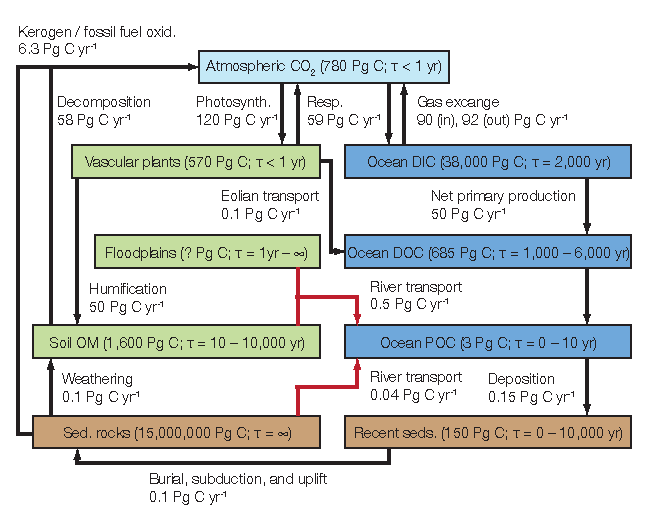
\includegraphics[]{Thesis_Figures/Ch1Fig1}}
	\caption[Carbon cycle reservoir inventories and fluxes]{Estimates of major reservoir inventories (in Pg C; $1$ Pg C = \SI{e15}{g.C}) and carbon fluxes (in \si{Pg.C.yr^{-1}}). Box colors correspond to the following reservoir types: light blue, atmosphere; dark blue, marine; green, terrestrial; brown, geologic. Riverine fluxes are highlighted in red. Figure modified from \citet{Bianchi:2011cu}.}
	\label{Ch1Fig:1}
\end{figure}

\subsection{The biospheric carbon cycle}

The major process by which carbon is transferred between biospheric reservoirs is the fixation of \ce{CO2} to biomass via photosynthesis and the corresponding respiration of organic matter back to \ce{CO2}:
%
% Equation 1
\begin{equation}\label{Ch1Eq:1}
	\ce{CO2 + H2O <=>[{photosynthesis}][{respiration}] CH2O + O2}
\end{equation}
%
where \ce{CH2O} represents organic carbon contained in biomass (OC\sub{bio}). Globally, if photosynthesis outpaces respiration, then this process results in a net increase in the size of surficial OC reservoirs and therefore a decrease in \textit{p}\ce{CO2}, while the opposite is also true. However, it is well known that the biosphere is highly self-contained, resulting in a near-perfect balance between photosynthetic \ce{CO2} fixation and subsequent respiration on a global scale \citep{Sarmiento:2006wz}. Despite this, small imbalances do persist, resulting in a "leaky" biosphere and the accumulation of OC\sub{bio} within marine sediments (Figure \ref{Ch1Fig:1}).

One process by which sedimentary OC accumulation can occur is the erosion of terrestrial landscapes and transport of particulate OC (POC) to coastal margin sediments via rivers \citep{Ludwig:1996ul,Schlunz:2000tl}. Although fluvial POC export flux represents only a small fraction of terrestrial net primary production \citep[\textit{i.e.} $\leq 1$\%;][]{Galy:2015fx}, this process continuously removes OC from the terrestrial biosphere that could have otherwise been respired. If this material subsequently escapes remineralization in marine sediments, as has been observed in many fluvial fan settings \citep{Derry:1996um,Burdige:2005tr,Galy:2007ev,Hilton:2008fo}, then riverine POC transport can constitute a quantitatively important atmospheric \ce{CO2} sink over geologic timescales. 

Because fluvial suspended sediment and POC fluxes are known to depend on geomorphology, hydrology, and river discharge \citep{Milliman:2011ug}, which is itself controlled by precipitation patterns \citep[\textit{e.g.}][]{Jian:2009bz}, this process describes a direct response of the carbon cycle to changing climate -- that is, riverine carbon export constitutes a climate feedback. Furthermore, POC yield depends on the rate at which river networks are able erode the landscape \citep{Ludwig:1996ul,Ludwig:1998ud,Galy:2015fx}. In addition to climatic factors, erosion rates strongly depend on geologic variables such as lithology, landscape slope, and tectonic uplift rate \citep{Dadson:2003kl,Milliman:2011ug,Hilton:2016dz}. Fluvial POC export therefore represents the intersection between hydrologic and geologic carbon cycle controls. However, the relative responses to changes in such controls remain largely elusive, hindering our ability to quantitatively reconstruct the role of fluvial climate feedbacks in the past and to predict future changes.

% Figure 2
\begin{figure}[t]
	\makebox[\textwidth][c]{\includegraphics[]{Thesis_Figures/Ch1Fig2}}
	\caption[Schematic representation of Earth's two carbon cycles]{Schematic interpretation of the two carbon cycles, including the hypothesized governing climatic and geologic mechanisms. Credit: Eric Taylor, WHOI Graphics Services.}
	\label{Ch1Fig:2}
\end{figure}

\subsection{The geologic carbon cycle}

In addition to the transport and burial of OC\sub{bio}, highly erosive river networks draining sedimentary lithologies incorporate a significant amount of rock-derived OC \citep[OC\sub{petro}; \textit{e.g.}][]{Hilton:2011jw,Galy:2015fx}. Because they integrate the slowly subducted and lithified marine sediments on timescales of millions to tens of millions of years (Figure \ref{Ch1Fig:2}), sedimentary rocks represent the largest global OC stock by nearly $3$ orders of magnitude (Figure \ref{Ch1Fig:1}). While the vast majority of this reservoir is effectively decoupled from surface processes on shorter timescales, respiration of exposed OC\sub{petro} during fluvial transit represents an atmospheric \ce{CO2} source \citep{Galy:2008ff,Bouchez:2010if,Hilton:2014dh}. Because OC\sub{petro} available for weathering is roughly double that of atmospheric \ce{CO2} \citep[\textit{i.e.} \SI{1100}{Pg.C} in the upper \SI{1}{m};][]{Copard:2007bf}, even a small perturbation in oxidation rates could lead to large changes in the resulting atmospheric \ce{CO2} flux. 

While it is currently estimated that the fluvial OC\sub{bio} export flux to the coastal ocean is $\approx 3\times$ greater than that of OC\sub{petro} \citep{Galy:2015fx}, quantifying atmospheric \ce{CO2} emissions due to OC\sub{petro} oxidation remains elusive \citep{Galy:2008ff,Bouchez:2010if,Hilton:2014dh}, largely due to the fact that the kinetic, environmental, and compositional controls on this flux are poorly constrained. For example, because there exist few measurements of oxidation rate constants \citep{Chang:1999vo}, it remains unknown if OC\sub{petro} weathering is limited by erosion rates or kinetic constraints, while the roles of partial oxidation \citep{Schillawski:2008ko} and OC\sub{petro} chemical composition \citep{Galy:2008ff} have additionally received little attention. Furthermore, the relative response of OC\sub{bio} burial and OC\sub{petro} oxidation to changing climatic and geologic processes is not fully understood. For example, it has been proposed that high runoff due to increased intensity and frequency of tropical storms during periods of elevated atmospheric \ce{CO2} should lead to increased export and burial of OC\sub{bio}, thereby lowering \textit{p}\ce{CO2} \citep[\textit{i.e.} a negative feedback loop;][]{Hilton:2008fo}. However, high runoff has also been shown to result in elevated sediment yield and denudation rates, potentially increasing the exposure rate of freshly uplifted OC\sub{petro} to weathering and resulting in a positive feedback \citep{Hilton:2014dh}.

The net effect of OC incorporation, transport, and evolution within fluvial systems on \textit{p}\ce{CO2} must therefore reflect the balance between \textit{(i)} burial of recently fixed OC\sub{bio} and \textit{(ii)} oxidation of eroded OC\sub{petro} (Figure \ref{Ch1Fig:2}). Constraining the response these two processes to both climatic and geologic perturbations is therefore a major motivating factor for this thesis.

\section{Motivation for this work}

\subsection{Constraining feedback mechanisms}

While critically important for understanding the global carbon cycle, quantifying modern fluvial fluxes alone (Figure \ref{Ch1Fig:1}) does not offer insight into the governing mechanisms that control OC source, transport, and fate. On the global scale, the importance of constraining such feedback mechanisms has long been recognized in order to reconstruct changes in atmospheric \ce{CO2} concentration over geologic timescales \citep{Berner:1999wj}. However, this has only recently been applied to modern fluvial systems. For example, recent studies \citep[\textit{e.g.}][]{Hilton:2008fo,Hilton:2012dt,Galy:2015fx} highlight the importance of erosive processes and sediment yield in determining both OC\sub{bio} and OC\sub{petro} export fluxes, suggesting that increased storm-driven erosion due to elevated \textit{p}\ce{CO2} could provide a negative feedback by increasing OC\sub{bio} burial in marine sediments.

Furthermore, it is now known that OC transport through river networks is not passive. Rather, fluvial transit integrates the complex interactions between multiple biogeochemical processes, each of which has the ability to alter the evolution of OC composition and quantity \citep{Cole:2007gp,Aufdenkampe:2011fm,Bianchi:2011cu}. This has lead to a new paradigm in our understanding of passive-margin systems in which OC is continuously deposited, chemically altered, and resuspended during transit \citep[the so-called "river continuum"; Figure \ref{Ch1Fig:3};][]{Blair:2012du}. In contrast, active-margin systems are now recognized not only as regions of intense erosion and OC\sub{bio} export, but also for OC\sub{petro} weathering due to uplift of OC-rich meta-sedimentary rocks \citep[Figure \ref{Ch1Fig:3};][]{Milliman:1992fu}. Therefore, based on this current understanding, passive-margin and active-margin systems should respond to environmental perturbations in fundamentally unique ways.

This thesis aims to advance our mechanistic understanding of fluvial carbon cycle feedbacks. To do so, I compare two end-member systems: \textit{(i)} the Congo River representing large, floodplain-dominated, and low-erosion environments in order to isolate climatic controls; and \textit{(ii)} rivers draining the highly erosive Central Range of Taiwan in order to determine geologic controls on active margins.

% Figure 3
\begin{figure}[t]
	\makebox[\textwidth][c]{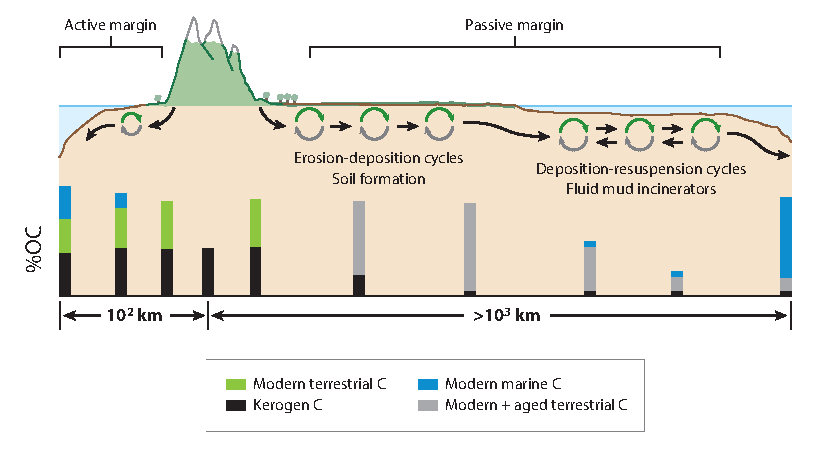
\includegraphics[]{Thesis_Figures/Ch1Fig3}}
	\caption[Schematic representation of the river continuum]{Schematic representation of fluvial particulate OC evolution in active-margin and passive-margin systems (\textit{i.e.} the river continuum). Figure modified from \citet{Blair:2012du}.}
	\label{Ch1Fig:3} 
\end{figure}

\subsection{The need for time-series measurements}

Fluvial systems are inherently dynamic in nature. However, there exist surprisingly few studies that consider riverine carbon export in a time-series manner, especially when including suspended sediments and particulate OC. Although such studies are logistically difficult, they provide critically important information regarding the seasonal variability and long-term evolution of river basins \citep[\textit{e.g.}][]{Peterson:2002hj,Raymond:2003fd,Milliman:2011ug,Voss:2015dd}. In addition to refining our estimates of carbon flux (Figure \ref{Ch1Fig:1}), time-series measurements have revealed that OC composition exhibits significant temporal variability that is related to hydrology \citep{Voss:2015dd,Hemingway:2016bq}. Furthermore, time-series studies provide a necessary link between the synoptic, "campaign-style" results that describe most of our knowledge on modern river systems and paleoclimate reconstructions utilizing sediments deposited in river-dominated margins. In this thesis, I attempt to further develop this emerging "time-variable river continuum" model by utilizing a 34-month time-series of monthly measurements on the Congo River in addition to a high-resolution (sub-daily) sampling scheme across three successive typhoon events in Taiwan. 

\subsection{Current methodological limitations}

Currently, most studies aimed at constraining the source and composition of exported fluvial OC utilize the following techniques: \textit{(i)} conservative tracers of bulk OC composition (\textit{e.g.} \ce{^{14}C} content, \ce{^{13}C} content, N/C ratios, \textit{etc.}); \textit{(ii)} compound-specific biomarker concentrations and isotope composition (\textit{e.g.} \textit{n}-alkyl lipds, sterols, lignin oxidation products); and \textit{(iii)} high-resolution non-quantitative mass spectrometry. When used in tandem, these techniques offer a powerful approach to understanding OC sources. 

However, each comes with its own drawbacks. For example, bulk measurements provide a weighted-average view of the composition of all OC contained within a sample, but require \textit{a priori} knowledge of end-member compositions in order to un-mix source contributions \citep{Perdue:2007fn,Weijers:2009iu,Hilton:2010cg,Hossler:2012jh}. In contrast, biomarker concentration and isotope measurements provide information specific to a particular OC source, but individual compounds typically constitute $\leq 1$\% of total OC and are subject to potentially large and unknown production biases \citep{Garcin:2014hg,Ponton:2014jr}. To address these drawbacks, a 4\super{th} class of organic geochemical techniques is emerging -- serial oxidation methods \citep[\textit{e.g.}][]{Rosenheim:2008ed,Follett:2014if,Beaupre:2016km}. In addition to geochemical applications using time-series fluvial sediments, this thesis aims to advance our theoretical understanding of one such serial oxidation technique -- the "Ramped PyrOx" (RPO) method. By heating a sample at a constant ramp rate and "binning" evolved \ce{CO2} for isotope measurements, this technique directly relates OC (thermo-)lability and isotope composition, and is therefore a promising method for monitoring OC degradation kinetics in the environment and for un-mixing OC sources.

\subsection{Thesis outline}

This thesis is motivated by a set of questions that aim to further our understanding of the environmental processes governing the role of rivers in the global carbon cycle. Thematically, these questions can be separated into two main sections:
%
\begin{enumerate}
%
\item \textbf{Ramped pyrolysis/oxidation (RPO) instrumental development, theory, data treatment, and post-processing} (Chapters \ref{Ch2} and \ref{Ch3}).
	\begin{itemize}
	%
	\item What is the contribution by contaminant ("blank") carbon in the RPO instrument, and how can this be corrected for? Does the RPO instrument impart any isotope fractionation?
	%
	\item Can profiles of OC thermal recalcitrance be related to intrinsic molecular properties, and what are the governing kinetic reactions?
	%
	\item How can RPO-derived thermal profiles and isotope results be combined to advance our understanding of OC sources and processing in the environment?  
	%
	\end{itemize}
%
\item \textbf{Application of organic geochemical methods to riverine suspended sediments and soils} (Chapters \ref{Ch4}, \ref{Ch5}, and \ref{Ch6}).
	%
	\begin{itemize}
	%
	\item How do the signals recorded in the fluvially exported POC integrate processes throughout the basin? Are they representative of upstream sources?
	%
	\item Do these signals respond to environmental variability (\textit{e.g.} hydrology, temperature) on seasonal and inter-annual timescales? How does this knowledge affect our interpretation of paleoenvironmental reconstructions using sedimentary archives?
	%
	\item How would changes in environmental conditions affect the stability of carbon reservoirs (\textit{e.g.} soils, rock-derived organic carbon) and the corresponding \ce{CO2} flux from these reservoirs to the atmosphere?
	%
	\end{itemize}
%
\end{enumerate}
%
In practice, this thesis is articulated around the following chapters:

\subsubsection{Chapter \ref{Ch2}}

This chapter describes recent developments to the RPO radiocarbon instrument located at the National Ocean Sciences Accelerator Mass Spectrometer (NOSAMS) facility. This method aims to separate individual components contained within complex OC mixtures based on thermo-lability and to evaluate the range of both stable carbon (\ce{^{13}C} and \ce{^{12}C}) and radiocarbon (\ce{^{14}C}) composition contained within a given sample. Here, the contribution and isotope composition of contaminant ("blank") carbon is constrained and corrected for. Additionally, the isotope fractionation due to mass-balance effects is determined based on a compilation of 66 samples that have been analyzed over \SI{\approx 4}{yr}, while the fractionation due to kinetic effects is evaluated using a set of standard reference materials. 

\subsubsection{Chapter \ref{Ch3}}

Here, a framework in which to interpret RPO isotope and kinetic results is proposed. OC decomposition kinetics are described as a continuous superposition of parallel first-order decay reactions that are governed by the Arrhenius equation. The distribution of activation energy required to explain observed thermal profiles is then constrained by solving the regularized inverse problem, thus relating RPO experimental results with intrinsic chemical properties of a given sample. To robustly verify the assumptions built into this model, a set of test samples was analyzed under a range of experimental conditions. Lastly, this chapter discusses how the RPO instrument presents a novel approach for separating carbon sources and understanding OC transformation processes.

\subsubsection{Chapter \ref{Ch4}}

This chapter concerns the seasonal and inter-annual variability of vascular-plant-derived biomarker concentrations and $\delta^{13}$C values exported from the Congo River. Changes in the composition of vascular plant lipids (\textit{n}-alkanes, \textit{n}-alcohols, and \textit{n}-alkanoic acids) extracted from fluvial sedimentary archives are commonly used as a tracer for changes in past ecosystem structure carbon export. However, few studies have monitored the role of inter-annual variability on these signals. Using a 34-month time-series collected from the Congo River at Brazzaville, this chapter shows that alkyl lipid compound classes variably track upstream ecosystems and that \textit{n}-alcohols and \textit{n}-alkanoic acids are more susceptible to seasonal variability than are \textit{n}-alkanes. 

\subsubsection{Chapter \ref{Ch5}}

Using the same Congo River sample set, this chapter constrains the source of exported particulate OC using bulk conservative tracers ($\delta^{13}$C, $\Delta^{14}$C, N/C) and microbial glycerol dialkyl glycerol tetraether (GDGT) biomarkers. Variability in POC sources is shown to be driven by inter-annual hydrodynamic variability, with exported POC being dominated by significantly pre-aged material eroded from the \textit{Cuvette Congolaise} swamp forest during periods of high northern-hemisphere discharge. Compared to published time-series data from an upstream tributary (Oubangui River), these results offer insight into the dilution and replacement of upstream POC by downstream sources during fluvial transit. Combined, Chapters \ref{Ch4} and \ref{Ch5} constrain the environmental processes governing Congo River POC export by highlighting the importance of seasonal and inter-annual hydrologic variability.

\subsubsection{Chapter \ref{Ch6}}

Lastly, using a combination of bulk measurements, alkanoic acid biomarkers, and RPO results, this chapter reveals that the oxidation of rock-derived OC in the highly erosive Central Range of Taiwan is governed by microbial processes, a phenomenon that has previously been observed in laboratory incubation experiments but has yet to be verified as quantitatively important in the field. Additionally, the resulting \ce{CO2} flux to the atmosphere is constrained to be roughly equal to that of \ce{CO2} drawdown due to silicate weathering and burial of biospheric OC in this system. Because microbial oxidation appears to be rapid, it is likely not kinetically limited and resulting \ce{CO2} fluxes are governed by the rate of exposure of bedrock material to the weathering front (\textit{i.e.} erosion rate).

% Chapter 2 text
\chapter{Assessing the blank carbon contribution, isotope mass balance, and kinetic isotope fractionation of the ramped pyrolysis/oxidation instrument at NOSAMS}
\label{Ch2}
\raggedbottom

{\let\thefootnote\relax\footnotetext{This chapter was originally published as: Hemingway J.D., Galy V.V., Gagnon A.R., Grant K.E., Rosengard S.Z., Soulet G., Zigah P.K., and McNichol A.P. (2017) {Assessing the blank carbon contribution, isotope mass balance, and kinetic isotope fractionation of the ramped pyrolysis/oxidation instrument at NOSAMS.} \emph{Radiocarbon} \textbf{under review.} }}

\clearpage

\section{Abstract}

We estimate the blank carbon mass over the course of a typical Ramped PyrOx (RPO) run ($150 - 1000$\textdegree C; $5$\textdegree C min\textsuperscript{-1}) to be $3.7 \pm 0.6$ $\mu$gC with an Fm value of $0.555 \pm 0.042$ and a \ce{\delta^{13}C} value of $-29.0 \pm 0.1$\textperthousand\ VPDB. Additionally, we provide equations for RPO Fm and \ce{\delta^{13}C} blank corrections, including associated error propagation. By comparing RPO mass-weighted mean and independently measured bulk \ce{\delta^{13}C} values for a compilation of environmental samples and standard reference materials (SRMs), we observe a small yet consistent \ce{^{13}C} depletion within the RPO instrument (mean -- bulk: $\mu = -0.8$\textperthousand; $\pm 1 \sigma$ = $0.9$\textperthousand; $n = 66$). In contrast, mass-weighted mean Fm values accurately match bulk measurements (mean -- bulk: $\mu = 0.005$; $\pm 1 \sigma$ = $0.014$; $n = 36$). Lastly, we show there exists no significant intra-sample \ce{\delta^{13}C} variability across carbonate SRM peaks, indicating minimal mass-dependent kinetic isotope fractionation during RPO analysis. These data are best explained by a difference in activation energy between \ce{^{12}C}- and \ce{^{13}C}-containing compounds (\ce{^{13-12}\Delta E}) of $0.3 - 1.8$ J mol\textsuperscript{-1}, suggesting that blank and mass-balance corrected RPO \ce{\delta^{13}C} values accurately retain carbon source isotope signals to within $1 - 2$\textperthousand.

\section{Introduction}

Thermoanalytical instruments such as thermogravimetry (TG) and pyrolysis gas chromatography (pyGC) are frequently used in petroleum geoscience \citep{Peters:1986uc}, biofuels research \citep{White:2011iz}, and soil science \citep{Plante:2009cp} to monitor the thermal reactivity of organic carbon (OC) contained within environmental samples. Additionally, petroleum geochemists have long coupled thermal analysis methods with isotope ratio measurements to investigate the origins and maturity of thermogenic hydrocarbons, leading to the development of techniques such as pyGC-isotope ratio mass spectrometry \citep[IRMS;][]{Galimov:1988vq,Berner:1996wn,Cramer:2004tg}. However, despite their potential to probe the relationship between OC molecular composition, isotope composition, and thermal reactivity, coupled thermal-isotope methods have found limited use in other fields of organic geochemistry. Still, preliminary studies analyzing environmental samples such as soils indicate that TG coupled with IRMS can yield meaningful trends in stable-carbon (\ce{^{12}C}, \ce{^{13}C}) composition with temperature \citep{LopezCapel:2006bc,LopezCapel:2008et}. Furthermore, \citet{Szidat:2004kx} and \citet{Currie:2005wo} successfully separated and determined the radiocarbon (\ce{^{14}C}) content of organic and elemental ("black") carbon fractions in aerosols using a stepped-temperature approach, confirming the possibility that thermal-isotope techniques can be used in tandem with radiocarbon analysis.

Recently, a novel instrument has been developed at NOSAMS to determine both the stable and radiocarbon isotope composition of evolved gases from environmental samples with increasing temperature \citep{Rosenheim:2008ed}. This method, termed "Ramped PyrOx" or "RPO", is increasingly being utilized in a host of environments to understand the relationship between carbon source, \ce{^{14}C} content, and thermal reactivity \citep[\textit{e.g.}][]{Rosenheim:2012kh,Plante:2013tu,Rosenheim:2013dka,Schreiner:2014jr,Bianchi:2015jr}. However, a complete understanding of isotope fractionation within the RPO instrument is currently lacking, hindering our ability to accurately interpret evolved-gas \ce{^{13}C} composition as a carbon source tracer. Additionally, RPO analysis shows promise for improving age-model constraints on carbonate-free sediments \citep{Rosenheim:2013va,Subt:2016dh}, although this application requires that contaminant ("blank") carbon contributions and \ce{^{14}C} mass balance are well constrained. Therefore, the aim of this study is to investigate the blank carbon contribution, isotope mass balance, and kinetic fractionation within the RPO instrument located at NOSAMS.

\section{Analytical Setup}

The NOSAMS RPO instrumental design is originally described in \citet{Rosenheim:2008ed} and has since been modified to lower contaminant carbon inputs by replacing all plumbing with copper tubing, improve gas flow rates, and improve temperature ramp stability \citep{Plante:2013tu}. In this setup, ultra-high purity (UHP) He gas flows at $32$ mL min\textsuperscript{-1} into a pre-combusted ($850$\textdegree C, 5 hours) quartz reactor sitting in a two-stage oven containing sample material to be pyrolyzed/oxidized (Figure \ref{Ch2Fig:1}A--B). He gas is combined with $3$ mL min\textsuperscript{-1} UHP O\textsubscript{2} either $(i)$ prior to entering the quartz reactor ("oxidation mode") or $(ii)$ downstream of sample material but upstream of a Cu, Pt, and Ni wire catalyst via a reactor side-arm ("pyrolysis mode"). An optimized, combined flow rate of $35$ mL min\textsuperscript{-1} was chosen to minimize transfer time within the system while still allowing sufficient contact time with the wire catalyst and complete cryogenic trapping of CO\textsubscript{2}. During a run, the lower oven containing the catalyst is held at $800$\textdegree C to facilitate oxidation of reduced carbon-containing gases to \ce{CO2}, while the upper oven containing the sample is ramped at a user-defined rate with $\approx 5$\% precision (typically $5 \pm 0.2$\textdegree C min\textsuperscript{-1}). We note that care must be taken when analyzing HCl-fumigated soil/sediment samples \citep[\textit{e.g.}][]{Plante:2013tu} as well as marine sediments and dissolved OC, as residual chloride has been observed to interact with and melt the catalysis wire, thus blocking gas flow within the reactor.

After exiting the ovens, water vapor is removed using a dry ice and isopropanol slurry. Gases are then passed into an in-line Sable Systems\textsuperscript{\textregistered} CA-10 infrared gas analyzer (IRGA) where \ce{CO2} concentration (in parts per million by volume, ppm\ce{CO2}) is measured photometrically at 1-second resolution with $\approx 5$ ppm\ce{CO2} precision in order to generate a plot of temperature vs. \ce{CO2} concentration (termed a "thermogram"). Finally, gases are transferred to a toggling trap apparatus (Figure \ref{Ch2Fig:1}A, \ref{Ch2Fig:1}C--D) in which \ce{CO2} is frozen using liquid \ce{N2} while \ce{He} and \ce{O2} are vented to the atmosphere. At user-defined temperatures, the collecting trap is toggled and \ce{CO2} for each temperature window (termed a "fraction") is transferred to a vacuum line, quantified manometrically, and sealed into a pre-combusted ($525$\textdegree C, 1 hour) $6$ mm Pyrex\textsuperscript{\textregistered} tube containing $100$ mg \ce{CuO} and $10$ mg \ce{Ag} pellets. Following a run, tubes are re-combusted ($525$\textdegree C, 1 hour) to remove sulfur-containing contaminant gases and \ce{CO2} carbon isotopes are measured following standard NOSAMS procedures \citep{McNichol:1992tk,McNichol:1994dt,Pearson:1998vy}. Between each run, \ce{CO2} concentration measurements are calibrated using a 2-point calibration curve by plumbing $(i)$ UHP \ce{He} and $(ii)$ UHP \ce{He} containing a known \ce{CO2} concentration directly through the IRGA.

% Figure 1
\begin{figure}[t]
	\makebox[\textwidth][c]{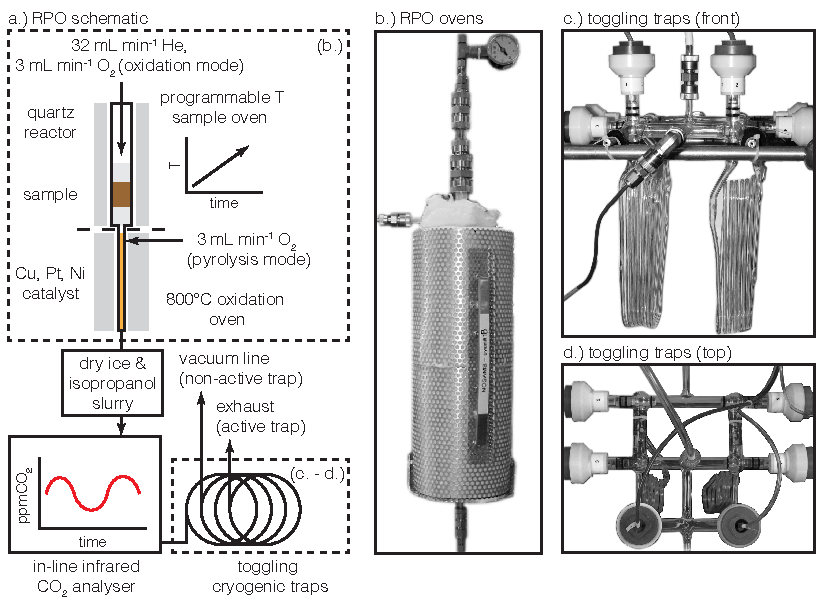
\includegraphics[]{Thesis_Figures/Ch2Fig1}}
	\caption[RPO instrumental setup and photos]{The NOSAMS RPO instrumental setup: \textit{(A)} schematic diagram, \textit{(B)} photo of the ovens, and \textit{(C)--(D)} photos of the toggling trap apparatus. Dashed boxes in panel \textit{(A)} indicate the regions shown in panels \textit{(B)--(D)}.}
	\label{Ch2Fig:1} 
\end{figure}

\section{Results and Discussion}

\subsection{NOSAMS RPO blank correction}

In order to estimate the RPO blank carbon mass and isotope composition, we directly trapped and analyzed \ce{CO2} eluted from empty, pre-combusted reactor inserts over the temperature range of a typical run ($150 - 1000$\textdegree C). Although blank carbon contribution is often determined by monitoring deflections from accepted standard reference material (SRM) isotope compositions \citep[\textit{i.e.} isotope dilution and "modern-dead" methods;][]{Pearson:1998vy,dosSantos:2007ca,Fernandez:2014gx,ShahWalter:2015iu}, the direct measurement method employed here is better-suited for the RPO instrument for the following reasons: 

\begin{enumerate}[label=(\textit{\roman*})]

\item Deflections from accepted SRM isotope values are only informative over the narrow temperature range in which the material decomposes, rather than over the course of an entire run.

\item For stable isotopes, it is possible that kinetic fractionation could overprint isotope deflections due to blank carbon contribution \citep[\textit{e.g.}][]{Cramer:2004tg,Dieckmann:2005dw}.

\item Isotope deflection methods are unable to separate blank carbon contributed within the quartz reactor \citep[\textit{i.e.} time-dependent blank carbon;][]{Fernandez:2014gx} from that contributed when switching the toggling trap apparatus \citep[\textit{i.e.} time-independent blank carbon;][]{Fernandez:2014gx}.

\end{enumerate}

To address point $(iii)$, we calculated the blank carbon mass and Fm value when the traps were toggled 0, 2, and 5 times between $150$ and $1000$\textdegree C. For 2- and 5-toggle runs, fractions were recombined within the vacuum line before transferring to a $6$ mm Pyrex tube to keep subsequent steps identical across all experimental conditions. Each experiment was performed in duplicate and the \ce{CO2} mass from each run was quantified separately before pairs were combined for ultra-small \ce{^{14}C} analysis \citep{ShahWalter:2015iu}. The 0-toggle experiment was repeated in duplicate for \ce{^{13}C} analysis using a dual-inlet IRMS as described in \citet{McNichol:1994dt}.

Resulting blank carbon mass is independent of the number of toggles throughout the run (Table \ref{Ch2Tab:1}), averaging $3.7 \pm 0.6$ $\mu$gC ($n = 8$) and indicating that the act of toggling the traps contributes a negligible amount of time-independent blank carbon. This is further supported by the near-identical Fm values across experimental conditions (Table \ref{Ch2Tab:1}). We therefore combine measurements from all experiments and calculate an average blank carbon Fm value of $0.555 \pm 0.042$ ($n = 3$). Similarly, we assume that the measured 0-toggle blank carbon \ce{\delta^{13}C} value of $-29.0 \pm 0.1$\textperthousand\ relative to Vienna Pee Dee Belemnite (VPDB; Table \ref{Ch2Tab:1}) is applicable regardless of the number of toggles.

% Table 1
\begin{sidewaystable}[p]
	\caption[RPO blank carbon mass, flux, and isotope composition]{NOSAMS RPO blank carbon mass, flux, and isotope composition. For measurements with $n = 1$, reported std. dev. is instrumental uncertainty. For measurements with $n = 2$, reported std. dev. is $\frac{1}{2}$ of the range between values.}
	\centering
		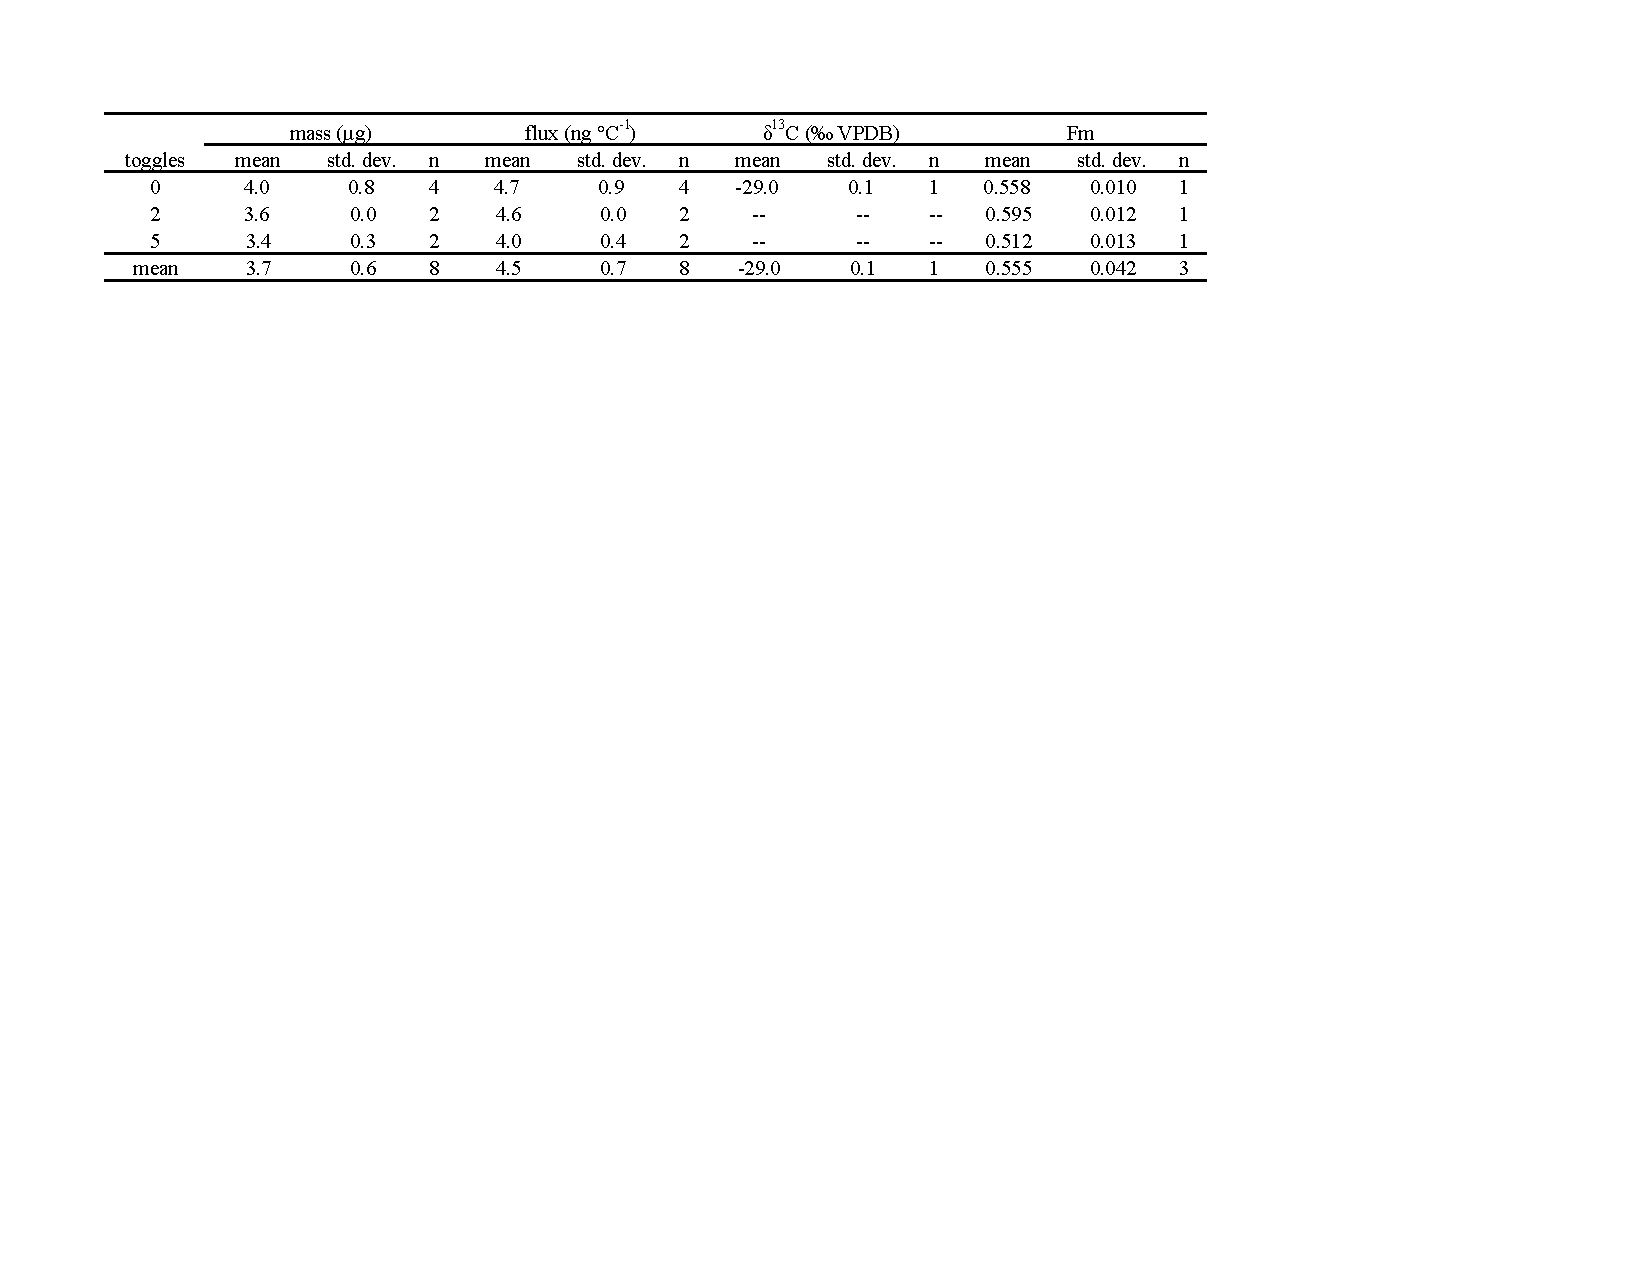
\includegraphics{Thesis_Tables/Ch2Tab1}
	\label{Ch2Tab:1}
\end{sidewaystable}

Blank carbon mass calculated here is significantly lower and less variable than that determined for a similar RPO system \citep[\textit{c.f.} $12.9 \pm 7.0$ $\mu$gC;][]{Fernandez:2014gx}, likely due to recent valve and plumbing upgrades on the NOSAMS instrument \citep{Plante:2013tu}. Additionally, photometric measurements suggest that time-dependent blank carbon contribution is not concentrated within any particular temperature range -- that is, there exist no distinct peaks in the blank thermograms (Figure \ref{Ch2Fig:2}). Although the mean blank flux appears to drop slightly above $500$\textdegree C, it can nonetheless be reasonably described as constant throughout the run within the 95\% confidence interval of the manometric measurements (Figure \ref{Ch2Fig:2}). Dividing the blank carbon mass by the experimental temperature range results in a blank carbon flux of $4.5 \pm 0.7$ ngC \textdegree C\textsuperscript{-1} (assuming a $5$\textdegree C min\textsuperscript{-1} ramp rate; Table \ref{Ch2Tab:1}). We therefore correct the mass of carbon in each RPO fraction for blank contribution according to:

% Equation 1
\begin{equation}\label{Ch2Eq:1}
m_{s} = m_{m} - \phi_{b} \Delta T
\end{equation}

where $m_{s}$ is the true sample carbon mass, $m_{m}$ is the measured carbon mass, $\phi_{b}$ is the blank carbon flux (in units of mass \textdegree C\textsuperscript{-1}), and $\Delta T$ is the temperature range over which the \ce{CO2} was collected. Additionally, we propagate uncertainty for this correction according to:

% Equation 2
\begin{equation}\label{Ch2Eq:2}
\sigma_{m_{s}} = \sqrt{ \left( \sigma_{m_{m}} \right)^2 + \left( \sigma_{\phi_{b}} \Delta T \right)^2}
\end{equation}
 
where $\sigma$ is the standard deviation associated with each subscripted measurement. This assumes that $\Delta T$ is known perfectly (\textit{i.e.} $\Delta T \equiv 0.0$) and that the uncertainty in $m_{m}$ and $\phi_{b}$ are uncorrelated, which is reasonable given that $m_{s} \approx m_{m} >> \Delta T \phi_{b}$. Similarly, we treat the measured \ce{CO2} isotope composition as a weighted average of sample carbon and blank carbon, and correct for blank contribution following:

% Equation 3
\begin{equation}\label{Ch2Eq:3}
\ce{^{x}R}_{s} = \frac{m_{m} \ce{^{x}R}_{m} - \phi_{b} \Delta T \ce{^{x}R}_{b}}{m_{s}}
\end{equation}

where $\ce{^{x}R}_{i}$ is the $\ce{^{x}C}/\ce{^{12}C}$ isotope ratio of component $i$ [$x$ = 13, 14; $i$ = (s)ample, (m)easured, (b)lank], with $\ce{^{13}R}_{i}$ expressed in \ce{\delta^{13}C} notation (\textperthousand\ VPDB) and $\ce{^{14}R}_{i}$ expressed in Fm notation \citep{Stuiver:1977uh,Reimer:2004th}. Lastly, we propagate uncertainty associated with isotope corrections. Because $m_{s} \approx m_{m}$, we cancel these where appropriate to avoid large covariance terms, leading to the equation:

% Equation 4
\begin{equation}\label{Ch2Eq:4}
\sigma_{\ce{^{x}R}_{s}} \approx \sqrt{\left( \sigma_{\ce{^{x}R}_{m}} \right)^2 + \left( \frac{\Delta T \ce{^{x}R}_{b}}{m_{s}} \sigma_{\phi_{b}} \right)^2 + \left( \frac{\phi_{b} \Delta T}{m_{s}} \sigma_{\ce{^{x}R}_{b}} \right)^2 + \left( \frac{\phi_{b} \Delta T \ce{^{x}R}_{b}}{m_{s}^{2}} \sigma_{m_{s}} \right)^2}
\end{equation}

For typical RPO fraction \ce{CO2} masses ($\approx 100$ $\mu$gC) and $\Delta T$ ($\approx 100$\textdegree C) encountered during sample runs, blank carbon correction shifts \ce{\delta^{13}C} values by $-0.02$ (for $\ce{\delta^{13}C} = -35$\textperthousand\ VPDB) to $+0.15$\textperthousand\ (for $\ce{\delta^{13}C} = +5$\textperthousand\ VPDB) and Fm values by $-0.002$ (for Fm = $0.01$) to $+0.002$ (for Fm = $1.0$), within the typical analytical uncertainty of these measurements. While \ce{^{14}C} content of graphite targets containing as little as $6$ $\mu$gC has been accurately analyzed at NOSAMS \citep{ShahWalter:2015iu}, we recommend a minimum RPO fraction mass of $25$ $\mu$gC in order to keep blank carbon corrections below $0.5$\textperthousand\ for \ce{\delta^{13}C} and $0.01$ for Fm (assuming $\Delta T = 100$\textdegree C). %A spreadsheet for performing all blank correction calculations is included in the supplementary material (Table S1).

% Figure 2
\begin{figure}[t]
	\makebox[\textwidth][c]{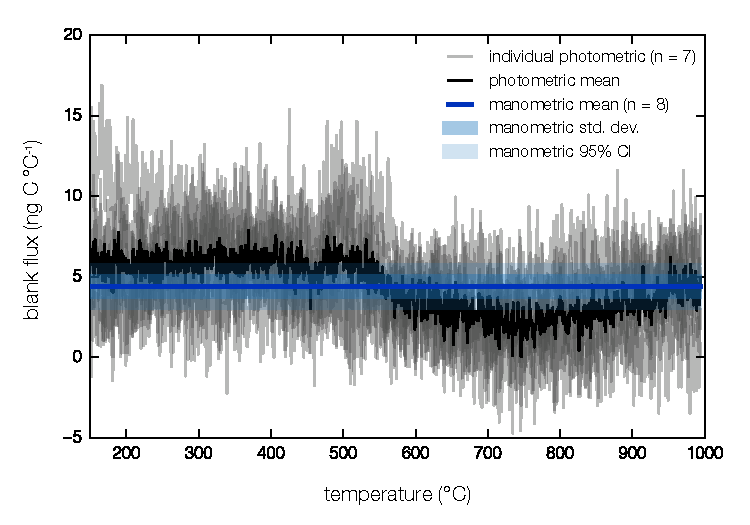
\includegraphics[]{Thesis_Figures/Ch2Fig2}}
	\caption[RPO blank carbon flux]{RPO blank carbon flux for a ramp rate of $5$\textdegree C min\textsuperscript{-1} as determined photometrically and manometrically. For photometric measurements, absolute \ce{CO2} concentrations were normalized such that the mean value for each run is equal to the manometric mean, as small differences in IRGA baseline calibration between runs leads to large changes in calculated blank flux. Still, photometric measurements are consistent with a constant flux throughout the run.}
	\label{Ch2Fig:2} 
\end{figure}

\subsection{Isotope mass balance}

If sample carbon is completely converted to \ce{CO2} by the end of a run and is efficiently transferred to the vacuum line, the mass-weighted mean \ce{CO2} isotope composition of blank-corrected RPO fractions should match independently measured bulk values within analytical uncertainty. To test this, we compare RPO mass-weighted mean compositions with bulk measurements for a range of sample types (SRMs, dissolved organic carbon, fluvial/marine total suspended sediments, soils, and lacustrine/marine sediments). Bulk \ce{\delta^{13}C} values were obtained either using an elemental analyzer coupled to a continuous-flow IRMS following \citet{Whiteside:2011jea} or on a dual-inlet IRMS after conversion to \ce{CO2} by closed-tube combustion as described in \citet{McNichol:1994dt}. Bulk Fm was measured at NOSAMS following standard preparation methods for each sample type \citep{McNichol:1994ty} and uncertainty for each bulk measurement is taken as the measured analytical uncertainty. We calculate RPO mass-weighted mean isotope compositions ($\mean{\ce{^{x}R}_{s}}$) as:

% Equation 5
\begin{equation}\label{Ch2Eq:5}
\mean{\ce{^{x}R}_{s}} = \Sigma_{j=1}^{n} f_{j} \ce{^{x}R}_{s,j}
\end{equation}

where $n$ is the total number of \ce{CO2} fractions collected throughout the run, $f_{j}$ is the contribution of fraction $j$ to the total mass of \ce{CO2} such that $\Sigma_{j=1}^{n} f_{j} \equiv 1.0$, and $\ce{^{x}R}_{s,j}$ is the blank-corrected $\ce{^{x}C}/\ce{^{12}C}$ isotope ratio of fraction $j$. Additionally, assuming that $f_{j}$ is known perfectly (\textit{i.e.} since $\Sigma_{j=1}^{n} f_{j}$ must equal $1.0$ by definition), we estimate the mass-weighted mean isotope uncertainty according to:

% Equation 6
\begin{equation}\label{Ch2Eq:6}
\sigma_{\mean{\ce{^{x}R}_{s}}} \approx \sqrt{ \Sigma_{j=1}^{n} \left( f_{j} \sigma_{\ce{^{x}R}_{s,j}} \right)^2}
\end{equation}

To test the ability of RPO mass-weighted mean isotope values to predict measured bulk values, we performed orthogonal distance regression (ODR), including uncertainty in both $x$ and $y$ variables, using the SciPy package in Python v3.5. and a weighting factor for each sample that is inversely proportional to the uncertainty in each measurement \citep{Boggs:1990wc,Oliphant:2007ud}. All data presented here are either taken from the literature \citep{Rosenheim:2012kh,Rosenheim:2013va} or are originally presented in this study.

% Figure 3
\begin{figure}[t]
	\makebox[\textwidth][c]{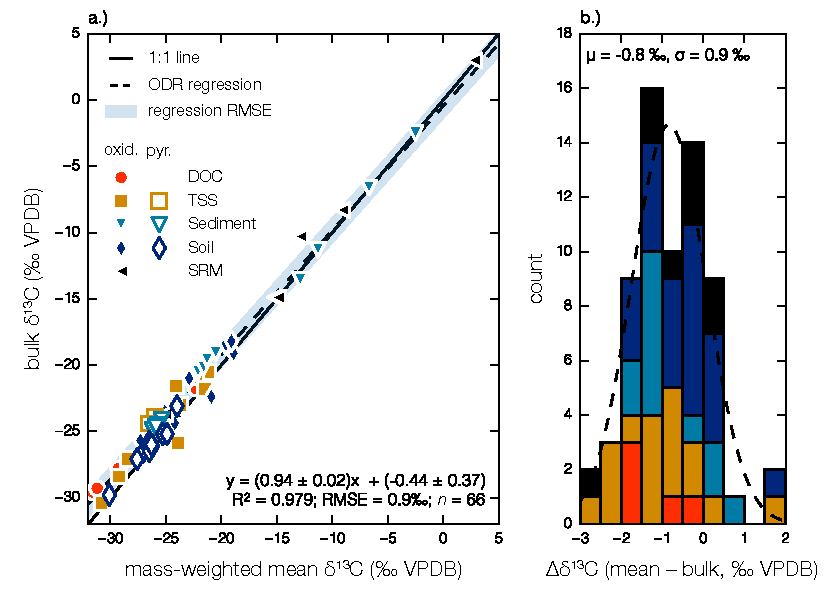
\includegraphics[]{Thesis_Figures/Ch2Fig3}}
	\caption[RPO \ce{\delta^{13}C} mass balance]{\textit{(A)} cross-plot of RPO mass-weighted mean vs. independently measured bulk \ce{\delta^{13}C} values for all samples in this study in which \ce{\delta^{13}C} data exist and \textit{(B)} the same data presented as a histogram of deviations from bulk values ($\Delta \ce{\delta^{13}C} = \ce{\delta^{13}C}_{\text{mean}} - \ce{\delta^{13}C}_{\text{bulk}}$). Sample abbreviations are as follows: DOC, dissolved organic carbon; TSS, total suspended sediments; SRM, standard reference material.}
	\label{Ch2Fig:3} 
\end{figure}

\subsubsection{Stable isotope mass balance}

On average, the RPO mass-weighted mean composition is depleted in \ce{^{13}C} by $0.8 \pm 0.9$\textperthousand\ relative to bulk measurements ($n = 66$), independent of RPO run conditions (Figure \ref{Ch2Fig:3}), as has been described previously \citep{Rosenheim:2012kh,Rosenheim:2013va}. To test if residual \ce{^{13}C}-enriched carbon remaining after RPO analysis could cause this depletion, \citet{Rosenheim:2012kh} re-quantified the carbon content of total suspended sediment samples after ramping to $1000$\textdegree C and determined that only $\approx 0.003$\% of initial carbon remained. Therefore, for the samples tested therein, \citet{Rosenheim:2012kh} concluded that low yield could not explain the observed bias. We tested additional potential sources of this depletion by performing a series of experiments using a \ce{CO2}:\ce{He} calibration gas mixture with known isotope composition ($465.5$ ppm\ce{CO2} in \ce{He}, $\ce{\delta^{13}C} = -14.9 \pm 0.04$\textperthousand\ VPDB) by:

\begin{enumerate}[label=(\textit{\roman*})]

\item Plumbing calibration gas directly into the toggling traps (bypassing the ovens of the RPO system) over a range of flow rates: $15$, $35$, and $50$ mL min\textsuperscript{-1}.

\item Freezing \ce{CO2} from the calibration gas for a range of integration times for each of the flow rates in experiment $(i)$: 1, 5, and 10 minutes.

\item Plumbing calibration gas through an empty, pre-combusted reactor insert and collecting \ce{CO2} between $150$ and $1000$\textdegree C, toggling every $170$\textdegree C for a total of 5 fractions (flow rate = $35$ mL min\textsuperscript{-1}, ramp rate = $5$\textdegree C min\textsuperscript{-1}).

\end{enumerate}

The results of experiments $(i)$ and $(ii)$ reveal that, for all flow rates and integration times, the collected \ce{CO2} \ce{\delta^{13}C} value ($-15.0 \pm 0.1$\textperthousand, $n = 9$) is statistically identical to the accepted value, indicating that dynamic cryogenic trapping within the toggling traps imparts no isotope fractionation. Furthermore, oven temperature does not appear to affect \ce{^{13}C} composition, as \ce{\delta^{13}C} values from all fractions in experiment $(iii)$ are statistically identical with a mean value of $-15.2 \pm 0.04$\textperthousand\ ($n = 5$). Although this is $0.3$\textperthousand\ depleted relative to the accepted value, this bias is smaller than that observed in most samples within our sample set (\textit{i.e.} up to $3$\textperthousand, Figure \ref{Ch2Fig:3}B), suggesting that any fractionation imparted during transport through the hot oven alone cannot cause observed \ce{^{13}C} depletion.

However, we note that the mass-weighted mean vs. bulk \ce{\delta^{13}C} difference is more pronounced in decarbonated samples containing exclusively OC (mean -- bulk: $\mu = -1.0$\textperthousand; $\pm 1\sigma =  0.9$\textperthousand; $n = 60$) as compared either to samples containing mixtures of carbonate and OC or pure carbonate SRMs (mean -- bulk: $\mu = -0.1$\textperthousand; $\pm 1\sigma =  0.5$\textperthousand; $n = 6$). We therefore hypothesize that isotope fractionation during OC degradation within the RPO oven could cause \ce{^{13}C} depletion, potentially due to incomplete oxidation to \ce{CO2} while reduced carbon-containing gases are in contact with the catalyst wire (Figure \ref{Ch2Fig:1}A). This mechanism is consistent with the results of experiment $(iii)$ indicating a lack of temperature dependence on isotope fractionation. We therefore recommend that \ce{\delta^{13}C} values of each RPO fraction $j$ within a particular sample can be fractionation-corrected according to the difference between mass-weighted mean and bulk measurements of that sample:

% Equation 7
\begin{equation}\label{Ch2Eq:7}
\ce{\delta^{13}C}_{s,j,\text{corrected}} = \ce{\delta^{13}C}_{s,j} + \left( \ce{\delta^{13}C}_{\text{bulk}} - \mean{\ce{\delta^{13}C}_{s}} \right)
\end{equation}

Furthermore, assuming that the covariance between $\ce{\delta^{13}C}_{s,j}$ for each fraction $j$ and the mass-weighted mean value ($\mean{\ce{\delta^{13}C}_{s}}$) is small compared to all other variance terms, we propagate uncertainty associated with fractionation correction according to:

% Equation 8
\begin{equation}\label{Ch2Eq:8}
\sigma_{\ce{\delta^{13}C}_{s, j, \text{corrected}}} \approx \sqrt{\sigma_{\ce{\delta^{13}C}_{s,j}}^2 + \sigma_{\ce{\delta^{13}C}_{\text{bulk}}}^2 + \sigma_{\mean{\ce{\delta^{13}C}_{s}}}^2 }
\end{equation}

\subsubsection{\ce{^{14}C} mass balance}

% Figure 4
\begin{figure}[t]
	\makebox[\textwidth][c]{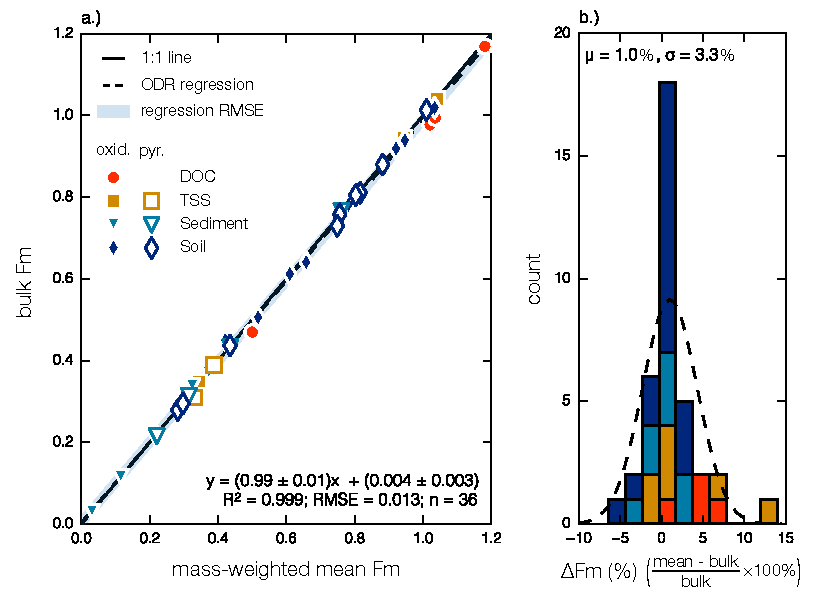
\includegraphics[]{Thesis_Figures/Ch2Fig4}}
	\caption[RPO Fm mass balance]{\textit{(A)} cross-plot of RPO mass-weighted mean vs. independently measured bulk Fm values for all samples in this study in which Fm data exist and \textit{(B)} the same data presented as a histogram of relative deviations from bulk values, in percent ($\Delta$Fm (\%) = $\frac{\text{Fm}_{\text{mean}} - \text{Fm}_{\text{bulk}}}{\text{Fm}_{\text{bulk}}} \times 100$\%). Sample abbreviations are as follows: DOC, dissolved organic carbon; TSS, total suspended sediments.}
	\label{Ch2Fig:4} 
\end{figure}

In contrast to \ce{^{13}C}, mass-weighted mean Fm values typically agree with bulk Fm values within analytical uncertainty across all sample types and run conditions (mean -- bulk: $\mu = 0.005$; $\pm 1 \sigma = 0.014$; $n = 36$; Figure \ref{Ch2Fig:4}). This can be easily explained because Fm is by definition corrected for the \ce{^{13}C}/\ce{^{12}C} ratio as measured on the AMS \citep{Stuiver:1977uh,dosSantos:2007ca} such that any mass-dependent fractionation occurring in the RPO instrument is accounted for. It is additionally useful to compare relative deviations between bulk and RPO mean values, as \ce{^{14}C} content of samples is highly variable. For the samples analyzed here, this equates to an average mean -- bulk relative difference of 1.0\% with a standard deviation of 3.3\% ($n = 36$), independent of absolute \ce{^{14}C} content of the sample (Figure \ref{Ch2Fig:4}B). This agreement between the mass-weighted mean Fm and bulk Fm values further precludes the possibility that a significant amount of isotopically unique carbon remains unreacted after ramping to $1000$\textdegree C, and is strong evidence that \ce{^{14}C} mass balance during RPO analysis is robust over the entire range of Fm values found in nature.

\subsection{Kinetic fractionation}

Finally, we evaluate the kinetic isotope effect (KIE) due to mass-dependent differences in pyrolysis/oxidation rates between each isotope during temperature ramping. If the amplitude of the KIE is significant relative to natural compositional differences, changes in \ce{\delta^{13}C} values between RPO fractions within a single sample could reflect instrumental fractionation rather than differences in carbon source isotope composition. Quantifying fractionation due to the KIE is therefore critical in order to interpret \ce{^{13}C} composition as a carbon source tracer. To do so, we measured \ce{\delta^{13}C} values of eluted \ce{CO2} from two carbonate SRMs in high-resolution fashion by toggling every $\approx 20$\textdegree C: $(i)$ travertine calcite \citep[IAEA C2;][]{Rozanski:1992vp} and $(ii)$ Icelandic spar (in-house standard; long-term average $\ce{\delta^{13}C} = 3.00 \pm 0.03$\textperthousand). Because carbonates are chemically and isotopically homogenous, any resulting \ce{\delta^{13}C} variability should follow a predictable, Rayleigh-like fractionation line that depends only on the difference in activation energy ($E$) between the decomposition of \ce{^{12}C}- and \ce{^{13}C}-containing molecules \citep[$^{13-12}\Delta E = \ce{^{13}E} - \ce{^{12}E}$;][]{Kwart:1982te}. We describe the carbonate decomposition rate constant at any temperature [k($T$)] by an Arrhenius equation (here written for \ce{^{12}C}):

% Equation 9
\begin{equation}\label{Ch2Eq:9}
\ce{^{12}k}(T) = \ce{^{12}k}_{0} \exp \left( - \frac{\ce{^{12}E}}{RT} \right)
\end{equation}

where $\ce{^{12}k}_{0}$ is the Arrhenius pre-exponential factor for \ce{^{12}C} and $R$ is the ideal gas constant. Following \citet{Kwart:1982te}, the KIE at any temperature [KIE($T$)] is defined as the ratio of \ce{^{12}C} and \ce{^{13}C} rate constants at that temperature: 

% Equation 10
\begin{equation}\label{Ch2Eq:10}
\text{KIE}(T) = \frac{\ce{^{12}k}(T)}{\ce{^{13}k}(T)} = \left( \frac{\ce{^{12}k}_{0}}{\ce{^{13}k}_{0}} \right) \exp \left( \frac{^{13-12}\Delta E}{RT} \right)
\end{equation}

Equation \ref{Ch2Eq:10} fundamentally states that, for a given \ce{^{13-12}\Delta E}, $\ce{^{12}k}_{0}$, and $\ce{^{13}k}_{0}$, KIE($T$) decreases with increasing $T$, indicating that kinetic fractionation within the RPO instrument will be largest for lower temperature components. Furthermore, we can reasonably assume that entropic differences between \ce{^{12}C}- and \ce{^{13}C}-containing molecules are negligible within the carbonate crystal lattice \citep[\textit{c.f.}][]{Tang:2000ua}. This assumption implies that $\ce{^{12}k}(T) = \ce{^{13}k}(T)$ as $T$ approaches infinity and requires that $\ce{^{12}k}_{0} = \ce{^{13}k}_{0} = k_{0}$ \citep{Cramer:2004tg}. Additionally, for each temperature we compute the \ce{^{13}C} composition of the remaining carbonate that has not yet decomposed [$\ce{^{13}R_{carb}}(T)$] as:

% Equation 11
\begin{equation}\label{Ch2Eq:11}
\ce{^{13}R_{carb}}(T) = \mean{\ce{^{13}R}_{s}} \exp \left( \frac{\ce{^{12}I}(T) - \ce{^{13}I}(T)}{\beta} \right)
\end{equation}

where $\beta$ is the oven ramp rate, $\mean{\ce{^{13}R}_{s}}$ is the mass-weighted mean \ce{^{13}C} content of the sample calculated by Equation \ref{Ch2Eq:5}, and $\ce{^{12}I}(T)$ and $\ce{^{13}I}(T)$ are the temperature integrals for \ce{^{12}C}- and \ce{^{13}C}-containing molecules according to \citet{Braun:1987vf} (here written for \ce{^{12}C}):

% Equation 12
\begin{equation}\label{Ch2Eq:12}
\ce{^{12}I}(T) \approx \frac{RT^2}{\ce{^{12}E}} \ce{^{12}k}(T) = \frac{k_{0}RT^2}{\ce{^{12}E}} \exp \left( - \frac{\ce{^{12}E}}{RT} \right)
\end{equation}

Finally, following \citet{Cramer:2004tg}, we calculate the predicted \ce{^{13}C} composition of instantaneously eluted \ce{CO2} at any temperature [$\ce{^{13}R_{CO_2}}(T)$]:

% Equation 13
\begin{equation}\label{Ch2Eq:13}
\ce{^{13}R_{CO_2}}(T) = \frac{\ce{^{13}R_{carb}}(T)}{\text{KIE}(T)} = \ce{^{13}R_{carb}}(T) \exp \left( - \frac{^{13-12}\Delta E}{RT} \right)
\end{equation}

Calculating $\ce{^{13}R_{CO_2}}(T)$ requires two inputs in addition to \ce{^{13-12}\Delta E}: $k_{0}$ and \ce{^{12}E}. Here we prescribe $k_{0}$ \textit{a priori} and estimate \ce{^{12}E} for each SRM by minimizing the root mean squared error (RMSE) between predicted first-order decay rates and observed thermograms using a Nelder-Mead algorithm in the SciPy package for Python v3.5. \citep[Table \ref{Ch2Tab:2};][]{Nelder:1965tk,Oliphant:2007ud}. We note that $\ce{^{13}R_{CO_2}}(T)$ is insensitive to our choice of $k_{0}$ \citep{Dieckmann:2005dw,White:2011iz}. For example, assuming a large \ce{^{13-12}\Delta E} value of $100$ J mol\textsuperscript{-1} for a peak at $700$\textdegree C, changing $k_{0}$ from $10^{10}$ sec\textsuperscript{-1} to $10^{20}$ sec\textsuperscript{-1} increases \ce{\delta^{13}C} of the first 1\% of eluted \ce{CO2} by only $1$\textperthousand\ and the first 50\% of eluted \ce{CO2} by only $0.2$\textperthousand. We therefore reasonably choose $k_{0} = 10^{15}$ sec\textsuperscript{-1} based on a compilation of literature values \citep[see][for review]{White:2011iz}. We then calculate \ce{^{13-12}\Delta E} that best predicts the \ce{^{13}C} composition of all \ce{CO2} fractions for each SRM by minimizing the measured vs. predicted RMSE \citep{Nelder:1965tk,Oliphant:2007ud}. To accurately compare instantaneous \ce{^{13}C} content predicted by Equation \ref{Ch2Eq:13} to measured RPO fractions (which integrate over time), we use the \ce{CO2}-mass-weighted average temperature for each fraction.

% Table 2
\begin{sidewaystable}[p]
	\caption[\ce{^{13-12}\Delta E} comparison between RPO and other instruments]{Comparison of $k_{0}$, \ce{^{12}E}, and \ce{^{13-12}\Delta E} values for carbonate SRMs in this study with those calculated using various thermoanalytical techniques on petroleum products \citep{Tang:2000ua,Cramer:2004tg,Tian:2007df}.}
	\centering
		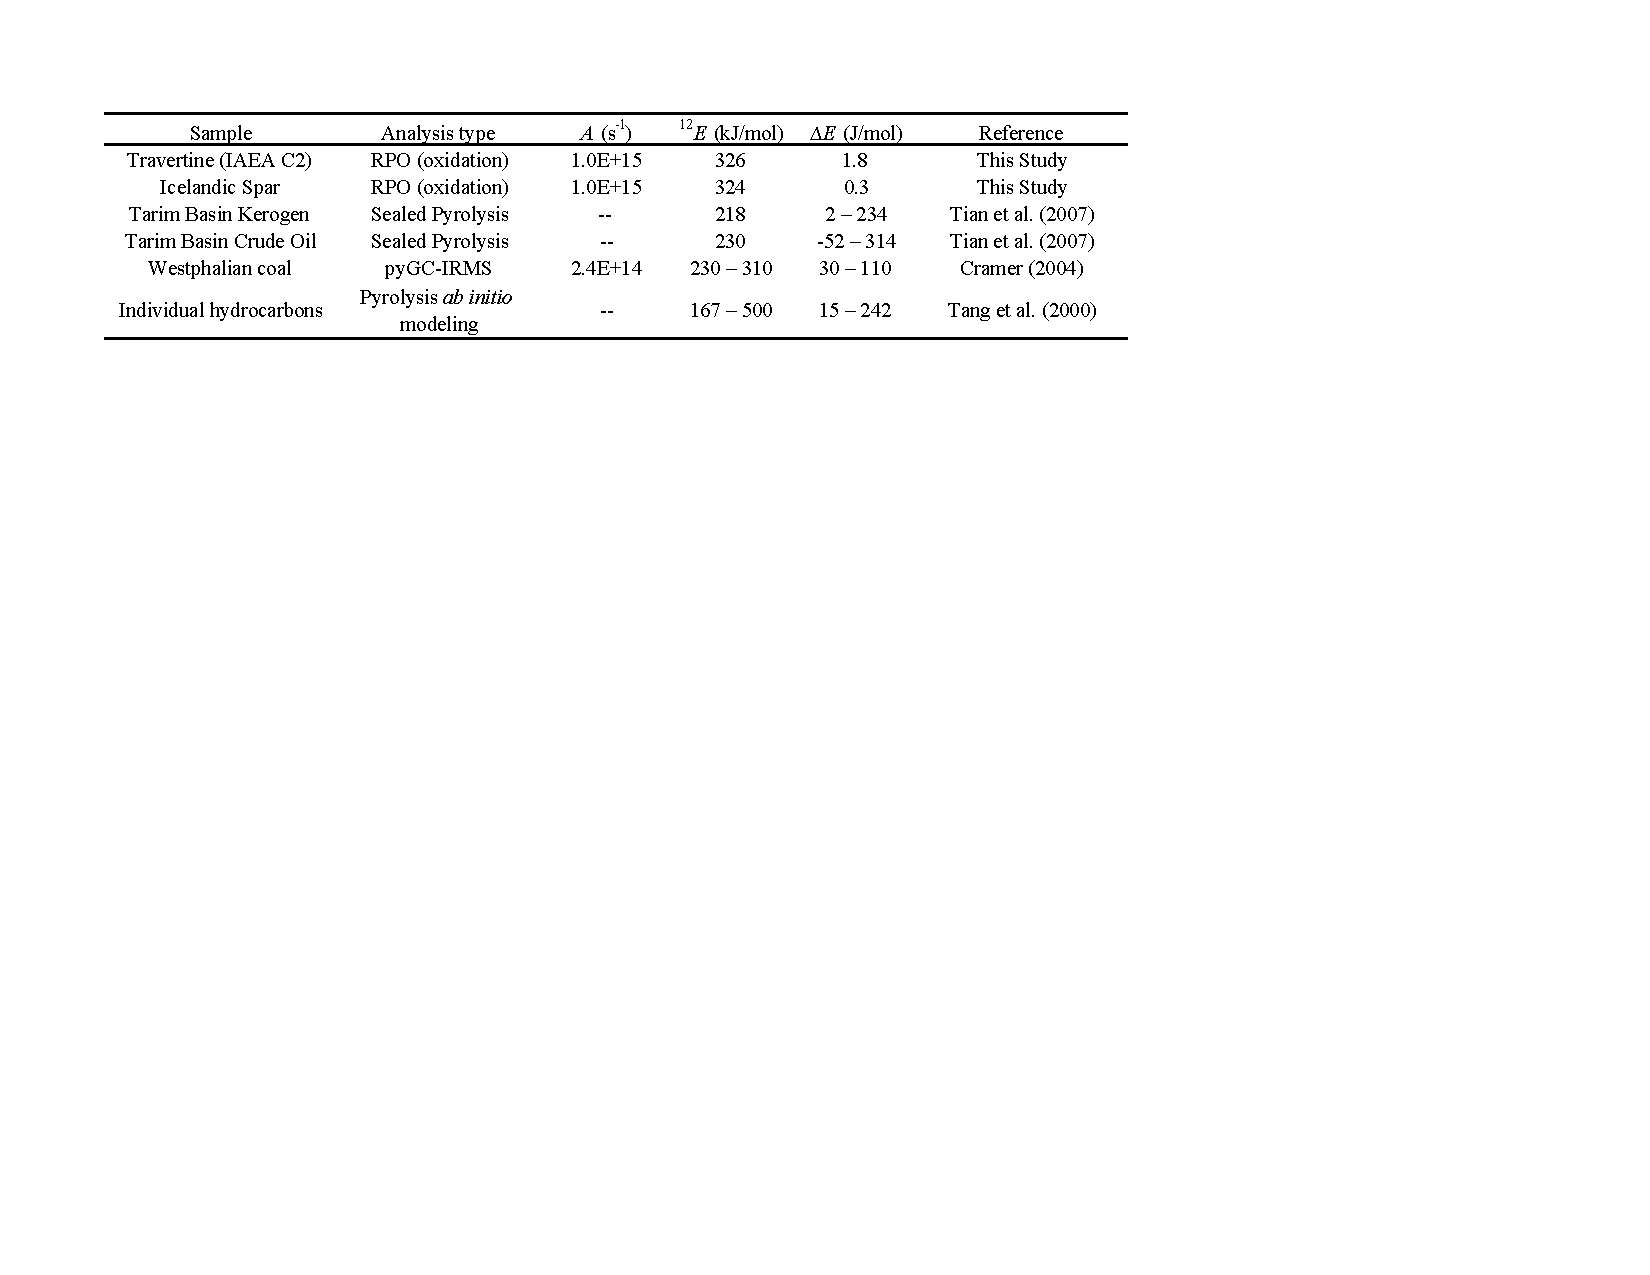
\includegraphics{Thesis_Tables/Ch2Tab2}
	\label{Ch2Tab:2} 
\end{sidewaystable}

Measured \ce{^{13}C} composition for both SRMs is consistent with a \ce{^{13-12}\Delta E} value between $0.3$ and $1.8$ J mol\textsuperscript{-1} (Table \ref{Ch2Tab:2}; Figure \ref{Ch2Fig:5}), significantly smaller than literature values for petroleum products using various non-isothermal pyrolysis instruments (Table \ref{Ch2Tab:2}). Therefore, for the SRMs analyzed here, predicted \ce{CO2} \ce{\delta^{13}C} increases by $<1$\textperthousand\ until $>>99$\% of initial carbon has been decomposed (Figure \ref{Ch2Fig:5}). However, we note that, on one hand, calculated \ce{^{13-12}\Delta E} using carbonate SRMs is likely a minimum estimate for environmental samples, as this carbon is already present in a +IV oxidation state, while oxidation of OC could increase \ce{^{13-12}\Delta E}. On the other hand, it has been shown that samples with high molecular diversity -- as is expected in environmental OC mixtures -- exhibit less apparent kinetic isotope fractionation than do single compounds such as the carbonates analyzed here \citep{Cramer:2004tg}. Overall, we recommend that a \ce{^{13-12}\Delta E} range of $0.3 - 1.8$ J mol\textsuperscript{-1} is valid for any component within an RPO run, and we consequently predict that kinetic isotope fractionation cannot exceed $1.8$\textperthousand\ during pyrolysis/oxidation of the first $99$\% of any sample eluting between $150$ and $1000$\textdegree C. In reality, \ce{^{13}C} enrichment at $>>99$\% combustion will never be observed during RPO analysis, as each fraction typically contains $10 - 20$\% of total carbon. We therefore conclude that \ce{\delta^{13}C} variability greater than $1 - 2$\textperthousand\ between RPO fractions must reflect differences in source carbon isotope composition.

% Figure 5
\begin{figure}[t]
	\makebox[\textwidth][c]{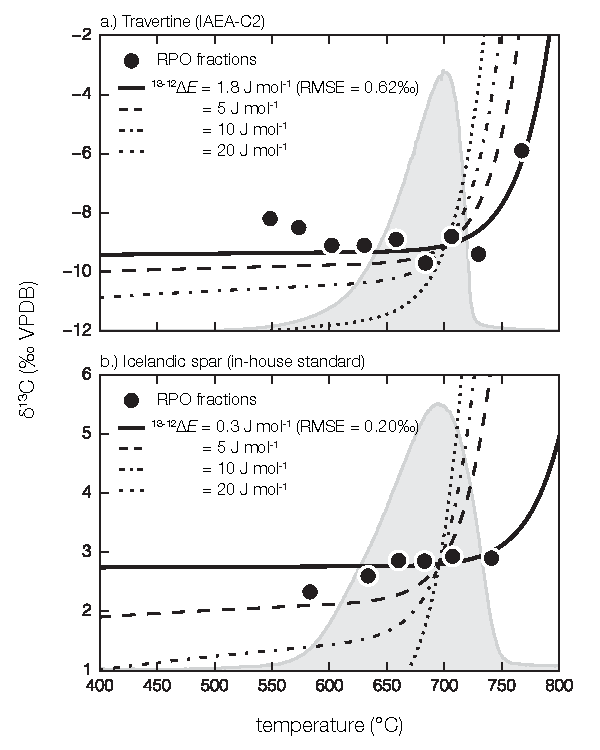
\includegraphics[]{Thesis_Figures/Ch2Fig5}}
	\caption[SRM kinetic isotope fractionation results]{RPO fraction \ce{\delta^{13}C} values for two carbonate SRMs [\textit{(A)} travertine and \textit{(B)} Icelandic spar] plotted with the predicted \ce{\delta^{13}C} value at each temperature using best-fit \ce{^{13-12}\Delta E} values from Equation \ref{Ch2Eq:13} (solid black line). For reference, predicted \ce{\delta^{13}C} values for various \ce{^{13-12}\Delta E} values are plotted as dashed and dotted lines, while shaded gray regions represent normalized thermograms (unitless). Each RPO fraction is plotted at its CO\textsubscript{2}-mass-weighted mean temperature.}
	\label{Ch2Fig:5} 
\end{figure}

Furthermore, if kinetic fractionation were driving observed \ce{^{13}C} variability, \ce{\delta^{13}C} values of eluted \ce{CO2} from all samples should increase monotonically with temperature along a trend that depends only on \ce{^{13-12}\Delta E}, which is clearly not observed. Rather, the \ce{\delta^{13}C} spread (\textit{i.e.} max -- min) across RPO fractions is highly variable between samples, reaching values as high as $28.8$\textperthousand\ in carbonate-containing lacustrine sediments and as low as $0.3$\textperthousand\ in decarbonated soils. For three carbonate-containing sediments analyzed here, we additionally measured the \ce{\delta^{13}C} value of total inorganic carbon following standard methods \citep{McNichol:1994ty} to compare with blank and mass-balance corrected RPO results. For all samples, high-temperature RPO \ce{\delta^{13}C} values agree with those of total inorganic carbon to within $1$\textperthousand, further indicating that RPO \ce{\delta^{13}C} values accurately reflect source carbon composition. 

Lastly, decreasing \ce{\delta^{13}C} values have been observed with increasing temperature in select samples such as decarbonated Ganges River total suspended sediments and Hawaiian soils (Figure \ref{Ch2Fig:6}), opposite of trends that would depict kinetic fractionation. Rather, this agrees with the interpretation that labile C\textsubscript{3} OC in these environments is replaced by \ce{^{13}C}-enriched, C\textsubscript{4}-derived material \citep{Chadwick:2007hc,Galy:2008jw}, and is further evidence that measured \ce{\delta^{13}C} trends reflect differences in carbon source isotope composition. Combined, the RPO \ce{\delta^{13}C} trends from environmental samples analyzed here agree with SRM-based fractionation predictions indicating that kinetic fractionation is small (\textit{i.e.} less than $1 - 2$\textperthousand) in the RPO instrument at NOSAMS.

% Figure 6
\begin{figure}[t]
	\makebox[\textwidth][c]{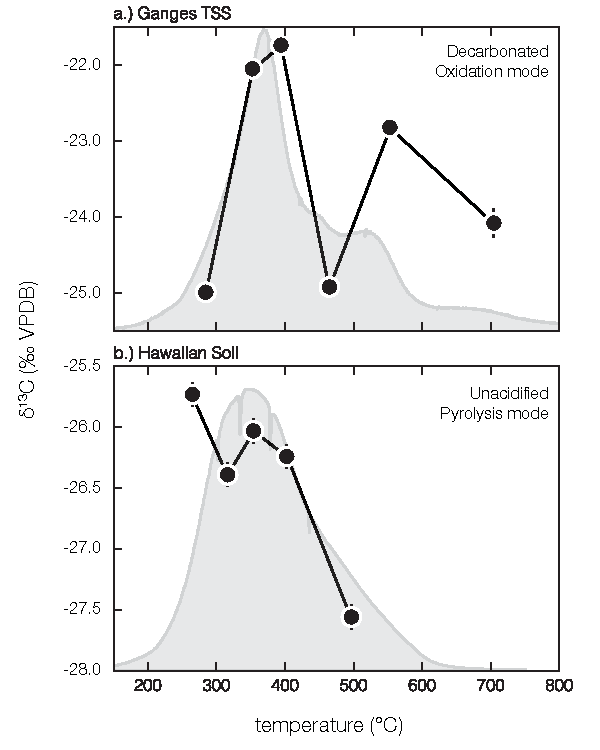
\includegraphics[]{Thesis_Figures/Ch2Fig6}}
	\caption[Samples exemplifying decreasing \ce{\delta^{13}C} with temperature]{RPO fraction \ce{\delta^{13}C} values for two environmental samples: \textit{(A)} decarbonated Ganges River TSS and \textit{(B)} Hawaiian soil. \ce{\delta^{13}C} values do not show a monotonic increase with temperature, precluding the possibility that \ce{^{13}C} variability in these samples reflects kinetic fractionation. For reference, shaded gray regions represent normalized thermograms (unitless). Each RPO fraction is plotted at its \ce{CO2}-mass-weighted mean temperature.}
	\label{Ch2Fig:6} 
\end{figure}

\section{Conclusion}

We describe the blank carbon composition, isotope mass balance, and kinetic isotope fractionation within the NOSAMS RPO instrument. Blank carbon mass is significantly smaller than that reported on a similar system \citep{Fernandez:2014gx} and can be described as a constant flux of $4.5 \pm 0.7$ ngC \textdegree C\textsuperscript{-1} (for a $5$\textdegree C min\textsuperscript{-1} ramp rate) with an Fm value of $0.555 \pm 0.042$ and a \ce{\delta^{13}C} value of $-29.0 \pm 0.1$\textperthousand. We find no evidence for significant time-independent blank contribution, likely due to recent valve and plumbing upgrades within the instrument \citep{Plante:2013tu}.

Isotope mass balance on a suite of environmental samples indicates that independently measured bulk Fm is accurately reconstructed using the RPO fraction mass-weighted mean. In contrast, RPO-predicted weighted-average \ce{\delta^{13}C} values are slightly depleted relative to measured bulk \ce{\delta^{13}C} values, especially for decarbonated samples containing exclusively OC. We eliminate the possibility that this depletion is due to low carbon yield or fractionation within the toggling traps. Rather, we hypothesize that this is caused by incomplete oxidation of reduced gases to \ce{CO2} within the oxidation oven and suggest that \ce{\delta^{13}C} of each RPO fraction for a given sample can be mass-balance corrected using the difference between measured bulk and mass-weighted mean values of that sample.

High-resolution \ce{\delta^{13}C} measurements on two carbonate SRMs suggest that kinetic isotope fractionation cannot exceed $1.8$\textperthousand\ in the RPO instrument. This agrees with intra-sample \ce{^{13}C} trends of the environmental samples analyzed for this study, which display a large range in \ce{\delta^{13}C} spread between fractions and are consistent with independently measured carbon source composition. Additionally, selected samples display \ce{^{13}C} trends with temperature opposite of that predicted by kinetic fractionation. These results are strong evidence that RPO kinetic fractionation is small and that blank and mass-balance corrected \ce{\delta^{13}C} values of each \ce{CO2} fraction reflect carbon source isotope composition to within $1 - 2$\textperthousand.

%\section{Acknowledgements}

%We thank Carl Johnson and the NOSAMS sample-prep lab staff for laboratory assistance. Instrumental improvements to the RPO system were largely the work of Steven Beaupr�. V.V.G. was partly supported by the US National Science Foundation (grants OCE-0851015 and OCE-0928582), the WHOI Coastal Ocean Institute (grant 27040213) and an Independent Study Award (grant 27005306) from WHOI; J.D.H. was partly supported by the NSF Graduate Research Fellowship Program under grant number 2012126152; G.S. and P.K.Z. were supported by the WHOI Postdoctoral Scholar Program with funding provided by NOSAMS.


%Part 2: Geochemical application
% Chapter 3 text
\chapter{An inverse model for relating organic carbon thermal reactivity and isotope composition using Ramped PyrOx}
\label{Ch3}
\raggedbottom

{\let\thefootnote\relax\footnotetext{This chapter is currently in preparation for submission as: Hemingway J.D., Rothman D.H., Rosengard, S.Z., Grant, K.E.,and Galy V.V. {An inverse model for relating organic carbon thermal reactivity and isotope composition using Ramped PyrOx.}}}

\clearpage

\section{Abstract}

Serial oxidation coupled with isotope ratio analysis (\ce{^{13}C}/\ce{^{12}C} and \ce{^{14}C}/\ce{^{12}C}, expressed as \ce{\delta^{13}C} and Fm) of eluted \ce{CO2} is a promising set of techniques for understanding the relationship between chemical composition, source, and residence time of organic carbon (OC) in the environment. However, a general treatment of oxidation kinetics is currently lacking. Here, we develop an inverse model to determine the nonparametric probability density function of OC thermal activation energy ($E$) contained within a given sample, $p_{0}(E)$, using the Ramped PyrOx (RPO) method. By analyzing a set of test samples representing various environments (fluvial suspended sediments, soils, marine sediments), we show that OC decay follows first-order kinetics and that our model results are independent of experimental conditions such as oven ramp rate. In contrast, decay kinetics of carbonate-rich samples cannot be accurately constrained, likely due to matrix effects and catalysis of \ce{CaCO3} decomposition during analysis.

Results indicate that samples with a large spread in \ce{\delta^{13}C} and Fm values between RPO fractions also contain a complex, broad $p_{0}(E)$ distribution due to the fact that they integrate over multiple OC sources with contrasting chemical and isotopic composition. We therefore propose that $p_{0}(E)$ is a useful metric for describing OC source and quality. To compare with isotope measurements, we calculate the average $E$ value contained in each RPO fraction by determining the temporal evolution of $p_{0}(E)$ throughout an experiment. For the samples analyzed here, results indicate that \ce{\delta^{13}C} and Fm vary linearly as a function of $E$, suggesting that OC bonding environment (as measured by thermal reactivity) is tightly coupled with isotope composition.

\section{Introduction}

The balance between organic carbon (OC) synthesis, remineralization to \ce{CO2}, and burial in soils/sediments exerts a significant control on the global carbon cycle on timescales of decades to millions of years \citep[\textit{e.g.}][]{Lasaga:1985ts,Derry:1996um,Hayes:2006ca,Galy:2008ff}. However, OC remineralization is not a straightforward process and depends on multiple complicating factors such as molecular diversity \citep{Kellerman:2015jn}, secondary chemical interactions \citep{Hedges:2000vh,Schmidt:2011gg}, physical protection by particles \citep{Mayer:1994wn,Mikutta:2006gx}, environmental conditions such as \ce{O2} exposure time \citep{Hartnett:1998id}, microbial diversity \citep{Kramer:2008dd,Janssens:2010hd,Schmidt:2011gg}, and microbial "priming" of recalcitrant material \citep{Bianchi:2011cu}. The relative importance of these factors is still actively debated and will likely vary depending on environmental conditions \citep[\textit{e.g.}][]{Hedges:2001ve,Rothman:2007jq,Schmidt:2011gg,Kellerman:2015jn}, thus hindering our ability to mechanistically understand and interpret the causes of observed heterogeneity in OC decay rates \citep{Boudreau:1991wf}.

To address this issue, a novel class of analytical techniques, broadly termed "serial oxidation" methods, has recently been developed. Such analyses separate compounds within a bulk sample based on various metrics of lability -- that is, susceptibility to remineralization by chemical hydrolysis \citep{Helfrich:2007ej}, \textit{uv} light \citep{Follett:2014if}, heat \citep{Szidat:2004kx,Currie:2005wo,Rosenheim:2008ed}, microbial respiration \citep{Beaupre:2016km}, \textit{etc.} -- and measure the stable carbon (\ce{^{13}C}/\ce{^{12}C}) and radiocarbon (\ce{^{14}C}/\ce{^{12}C}) ratios of evolved \ce{CO2}. By separating evolved \ce{CO2} into different "bins," isotopic information can be obtained for groups of compounds exhibiting similar physical and/or chemical properties. Serial oxidation is therefore a promising method to directly probe the relationship between OC molecular composition, source, and environmental residence time.

Like bulk measurements, serial oxidation techniques benefit from the fact that all carbon contained within a sample is analyzed, and results therefore reflect the entire complex OC mixture. This contrasts with compound-specific isotope methods used for tracing carbon source and fate, in which particular biomarkers thought to represent major OC components are analyzed \citep[\textit{e.g.} plant-wax lipids;][]{Hayes:1989us,Eglinton:1996ff,Sessions:1999vg}. However, biomarker compound classes typically constitute \SI{\leq 1}{\%} of total OC, and significant biases in production rates, preservation, and integration have recently been observed \citep{Garcin:2014hg,Hemingway:2016bq}. Furthermore, it has been shown that biomarker classes thought to track similar OC sources (\textit{i.e.} plant-wax lipids and lignin phenols) can display drastically different \ce{^{14}C} content \citep{Feng:2013il}, thus complicating their use as a tracer for OC residence time. Serial oxidation methods are able to circumvent this issue while still providing information related to the distribution of isotope ratios within a sample that is otherwise lost when considering only bulk averages \citep{Blair:2012du}.

However, a theoretical treatment of serial oxidation kinetics is generally lacking, thus hindering our ability to correlate experimental isotopic results with intrinsic molecular properties and reaction energetics. To address this issue, we develop a framework for relating OC thermal recalcitrance with its corresponding \ce{^{13}C} and \ce{^{14}C} content during ramped-temperature pyrolysis/oxidation (termed "Ramped PyrOx" or "RPO" analysis). This method, first described by \citet{Rosenheim:2008ed}, involves heating a sample at a controlled rate while continuously quantifying and collecting evolved \ce{CO2}, which is binned over user-defined time windows (termed "fractions") and analyzed for carbon isotope composition. RPO analysis has recently been used in a host of environmental settings including soils \citep{Plante:2013tu}, riverine sediments \citep{Rosenheim:2012kh,Rosenheim:2013dka,Schreiner:2014jr,Bianchi:2015jr}, and marine sediments \citep{Rosenheim:2013va,Subt:2016dh} to investigate the differences in \ce{^{13}C} and \ce{^{14}C} composition for various OC components contained within a single sample. Despite these promising initial results, quantitative interpretation has thus far been limited due to the fact that reaction kinetics within the RPO instrument remain unknown.

We describe degradation rates using an inverse implementation of the distributed activation energy model (DAEM) in which OC quality -- that is, susceptibility to thermal degradation -- is described by activation energy ($E$) \citep{Braun:1987vf,Burnham:1987ut,Cramer:2004tg}. Similar to the isothermal reactive continuum model \citep{Boudreau:1991wf,Forney:2012dr,Forney:2012hz}, the DAEM treats OC remineralization as a superposition of parallel first-order decay reactions that are described by a probability density function (pdf) of $E$. In contrast to many previous studies \citep[\textit{e.g.}][]{Lakshmanan:1994vs,Cai:2007hh,deCaprariis:2012jk}, our implementation does not require that $E$ follows a particular parametric form (\textit{e.g.} Gaussian), but rather estimates a nonparametric $E$ distribution for unreacted material remaining at any time. Furthermore, because DAEM-derived $E$ is an intrinsic property of a given chemical bonding environment (\textit{i.e.} it does not depend on experimental conditions such as temperature ramp rate), thermal recalcitrance can be reasonably viewed as a proxy for OC molecular composition and redox state. Therefore, by calculating a pdf of $E$ across each time window in which \ce{CO2} was collected, our method aims to directly compare the distribution of OC molecular and isotopic composition contained within a sample.

We emphasize that biogeochemical OC recalcitrance can differ from thermal OC recalcitrance due to the presence of catalysts, extracellular enzymes \citep{Sinsabaugh:2008il,Arnosti:2011iv}, interaction with \textit{uv} light \citep{Spencer:2009vl}, microbial priming \citep{Bianchi:2011cu}, \textit{etc.} within the environment. It is precisely these differences that offer insight into the biogeochemical mechanisms controlling the carbon cycle. For example, the loss of high-$E$, \ce{^{14}C}-free OC across a shale redox front or in a soil profile might represent preferential biological oxidation of highly condensed, rock-derived carbon despite the high chemical and thermal recalcitrance of these compounds \citep{Petsch:2001eq,Rethemeyer:2004cy,Marschner:2008eo}. Conversely, the persistence of low-$E$ material with steadily decreasing \ce{^{14}C} content in aging sediments could indicate physical-chemical protection of otherwise labile compounds \citep{Mayer:1994wn,Rothman:2007jq}. By comparing activation energy with isotope composition for each RPO fraction in a variety of environmental samples, our method aims to fundamentally address the following question: \textit{How, if at all, do biogeochemical processes decouple observed reservoir ages (as measured by \ce{^{14}C} content) from OC recalcitrance (as predicted by chemical bonding environment)?}

To test our theoretical description of RPO kinetics, we analyzed a set of three samples representing a range of environments: fluvial suspended sediments, marine sediments, and soils. By subjecting these samples to various experimental conditions, we are able to validate the assumptions of our model while also offering insight into potential limitations of this approach. Finally, we compare reaction energetics with RPO-derived isotope composition and interpret these relationships within the context of current carbon cycle knowledge.

\section{Materials and Methods}

\subsection{Sample selection and preparation}

As a representative fluvial sample, we chose suspended sediments collected from the surface of the Narayani River at the base of the Himalayas (\ang{27.70} N, \ang{84.43} E) that have been previously analyzed for bulk OC and plant-wax carbon isotopes \citep{Galy:2008jw,Galy:2011hk,Galy:2011ix}. Aliquots of this sample, henceforth referred to as "Narayani PB-60," were taken for RPO analysis from freeze-dried archived material and acidified under HCl fumes to remove carbonates as described in \citet{Whiteside:2011jea}. Because residual chloride has been shown to interact with the RPO catalyst wire \citep{Hemingway:2016rc}, acidified aliquots were rinsed $3\times$ in \SI{18.2}{M \ohm} MilliQ water and freeze-dried overnight at \SI{-40}{\celsius} prior to analysis. For consistency and to properly calculate RPO isotope mass balance, organic carbon content (\%OC), \ce{^{13}C} composition, and \ce{^{14}C} composition were re-measured using fumigated and rinsed material following the methods of \citet{McNichol:1994dt,McNichol:1994ty}.

To represent marine sediments, we chose a carbonate-rich sample collected from the Southern Ocean (\ang{60.24} S, \ang{170.19} W) as part of the Joint Global Ocean Flux Study \citep[JGOFS;][]{Sayles:2001ua}. Aliquots were taken from archived core-top material (\SIrange{0}{0.5}{cm}, stored at \SI{-80}{\celsius}), freeze-dried overnight at \SI{-40}{\celsius}, and homogenized prior to RPO analysis. Inorganic carbon content (\%IC), \%OC, and bulk \ce{^{13}C} composition were re-quantified following \citet{McNichol:1994dt}. This sample, henceforth referred to as "JGOFS MC-1," was analyzed without acidification in order to investigate the effect of carbonates on RPO results.

Lastly, we analyzed a soil sample overlaying the Pololu lava flow located on the Kohala Peninsula of Hawaii \citep[\ang{20.15} N, \ang{155.83} W;][]{Chadwick:2007hc}. Archived material (freeze-dried, \SIrange{70}{90}{cm} depth) was homogenized and aliquots were taken for RPO analysis. Because this sample, henceforth referred to as "Pololu 4169," overlies igneous bedrock and does not contain petrogenic carbonates, acidification was not required. Bulk \%OC and \ce{^{13}C} content was measured using a Thermo Delta\super{V} elemental analyzer-isotope ratio mass spectrometer and bulk \ce{^{14}C} content was measured following \citet{McNichol:1994ty}.

\subsection{Ramped PyrOx analysis}

The RPO analytical setup has been described in detail previously \citep{Rosenheim:2008ed,Hemingway:2016rc}. In summary, a solid sample is loaded into a pre-combusted (\SI{850}{\celsius}, 5 hours) quartz reactor and placed into a two-stage oven (Figure \ref{Ch3Fig:1}). The reactor is then sealed and the sample is exposed to an atmosphere of $92$:$8$ \ce{He}:\ce{O2} with a flow rate of \SI{35}{mL.min^{-1}}, resulting in oxidative carbon combustion \citep[\textit{c.f.} pyrolysis as described in][]{Rosenheim:2008ed}. \ce{O2} is provided in excess to ensure that degradation kinetics do not depend on \ce{O2} concentration. During analysis, the oven surrounding the sample is programmed to heat at a user-defined ramp rate ($\beta$, see Table \ref{Ch3Tab:1} for symbol descriptions) and instantaneous temperature within the oven is measured using two thermocouples separated by \SI{\approx 1}{cm} to monitor temperature heterogeneity, which is typically \SI{< 5}{\celsius}. Following standard practice \citep{Rosenheim:2008ed}, a ramp rate of $\beta = 5$ \si{\celsius.min^{-1}} was used for all experiments in which \ce{CO2} gas was collected for isotope analysis in this study. In the second (downstream) oven, eluent gas is passed over a Cu, Pt, and Ni catalyst wire held at \SI{800}{\celsius} to facilitate oxidation of reduced carbon-containing gases to \ce{CO2}. 

After exiting the second oven, eluent gas is distilled through a water trap and passed into a flow-through infrared gas analyzer (IRGA) to measure \ce{CO2} concentration (in parts per million by volume; \si{ppm.\ce{CO2}}) with 1-second temporal resolution (resulting \si{ppm.\ce{CO2}} vs. temperature plots are referred to as "thermograms"). IRGA measurements are calibrated using a two-point calibration curve before each analysis to account for instrument drift, and are precise to within \SI{\pm 5}{ppm.\ce{CO2}} \citep{Hemingway:2016rc}. Downstream of the IRGA, eluent gas is passed into one of two switchable traps and \ce{CO2} is cryogenically frozen while He and \ce{O2} are vented to the atmosphere. Traps are switched at user-defined time points and \ce{CO2} is further distilled, quantified, transferred into glass tubes packed with \SI{\approx 100}{mg.\ce{CuO}} and \si{\approx 10}{mg.\ce{Ag}}, and flame sealed. 

% Figure 1
\begin{figure}[t]
	\makebox[\textwidth][c]{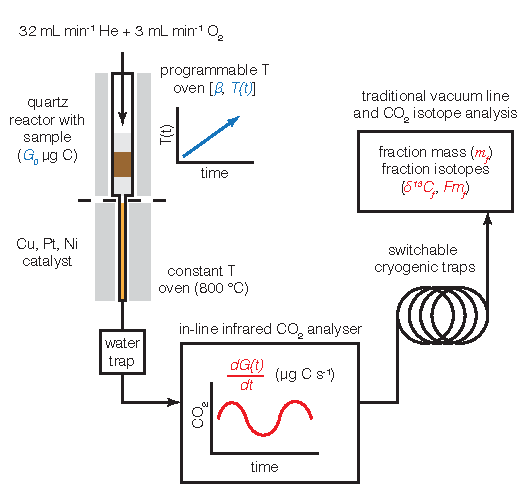
\includegraphics[]{Thesis_Figures/Ch3Fig1}}
	\caption[Schematic of the RPO instrumental setup]{Schematic of the RPO instrumental setup. User-defined inputs are printed in blue, while resulting observed measurements are printed in red (See Table \ref{Ch3Tab:1} for symbol definitions). }
	\label{Ch3Fig:1} 
\end{figure}

% Table 1
\begin{table}[p]
	\caption[List of mathematical symbols used throughout this study]{List of mathematical symbols used throughout this study.}
	\centering
		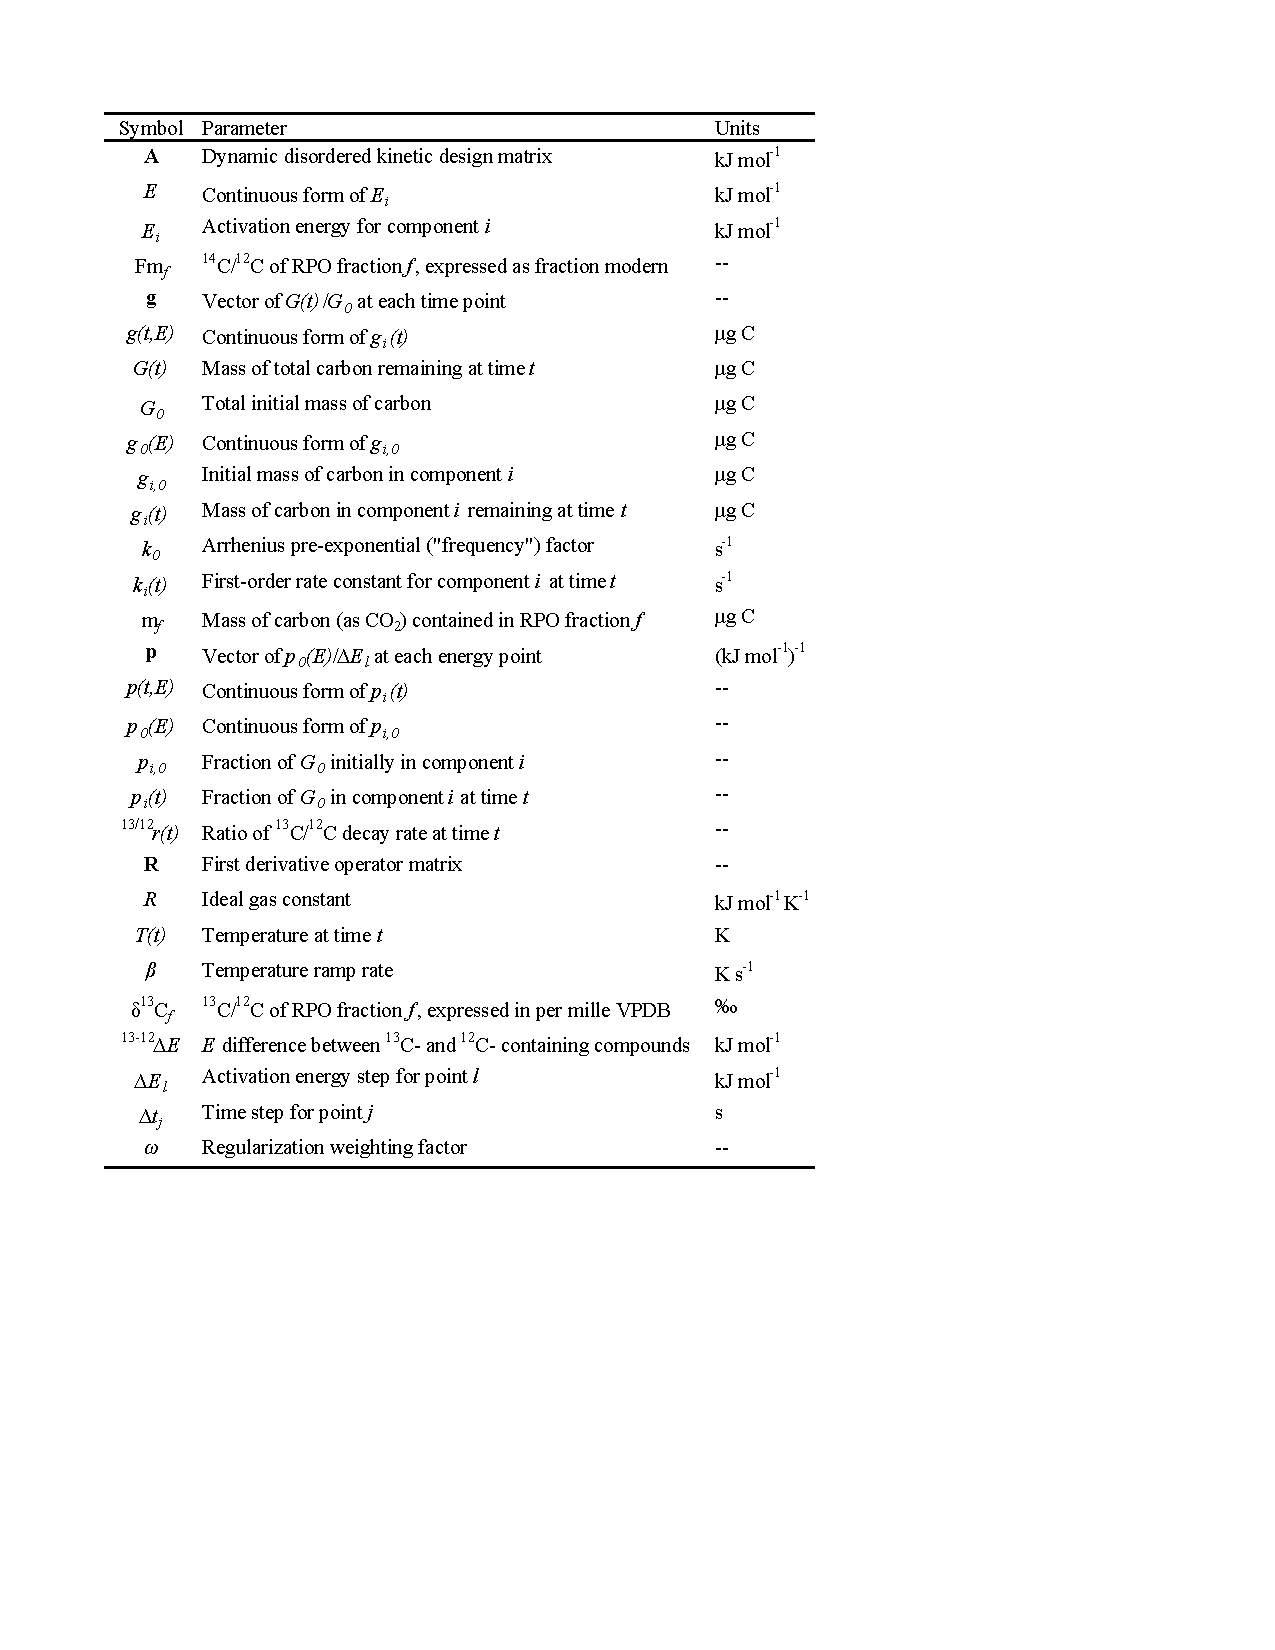
\includegraphics{Thesis_Tables/Ch3Tab1}
	\label{Ch3Tab:1} 
\end{table}

\subsection{Isotope measurement, blank correction, and data processing}

After recombustion at \SI{525}{\celsius} for 1 hour to remove trace contaminant gases, isotope composition of \ce{CO2} contained in each RPO fraction was analyzed following standard procedures \citep{McNichol:1994ty,Pearson:1998vy}, where \ce{^{13}C} content is expressed in \ce{\delta^{13}C} per mille (\si{\permil}) notation relative to Vienna Pee Dee Belemnite (VPDB) and \ce{^{14}C} content is expressed in fraction modern (Fm) notation following \citet{Stuiver:1977uh}. We note that Fm as reported here is identical to the "\ce{^{14}a_{N}}" notation of \citet{Mook:1999vf} as well as the "\ce{F^{14}C}" notation of \citet{Reimer:2004th}. RPO fraction masses, \ce{\delta^{13}C} values, and Fm values were corrected for blank carbon contribution, and \ce{\delta^{13}C} was additionally corrected to ensure \ce{^{13}C} mass balance as incomplete oxidation to \ce{CO2} has been shown to exhibit a small fractionation effect \citep{Hemingway:2016rc}. Analytical uncertainty was propagated throughout all corrections.

All calculations contained herein were performed using the open-source 'rampedpyrox' package for Python v.3.5 as described in \citet{Hemingway:bA3-kvLz}.

\section{Results}

RPO fraction temperature ranges, \ce{CO2} masses, \ce{\delta^{13}C}, and Fm are reported in Tables \ref{Ch3Tab:2}--\ref{Ch3Tab:4} along with independently measured bulk isotope composition for each sample. The resulting Narayani PB-60 thermogram can be described as a bimodal distribution with peaks at \SI{365}{\celsius} and \SI{662}{\celsius}, similar to that observed previously when analyzed in pyrolysis mode \citep[Figure \ref{Ch3Fig:2}A;][]{Rosenheim:2012kh}. Corresponding RPO fraction Fm values decrease monotonically between \SI{150}{\celsius} and \SI{725}{\celsius} from \num{0.891 \pm 0.004} (fraction 1) to \num{0.014 \pm 0.002} (fraction 8), followed by a small yet statistically significant increase to \num{0.042 \pm 0.002} in the final fraction. \ce{\delta^{13}C} values display the opposite trend, rising from \SI{-29.5 \pm 0.2}{\permil.VPDB} (fraction 1) to \SI{-21.8 \pm 0.2}{\permil.VPDB} (fraction 8) followed by a slight decrease to \SI{-23.5 \pm 0.2}{\permil.VPDB}. 

% Table 2
\begin{sidewaystable}[p]
	\caption[Narayani PB-60 RPO results]{Narayani PB-60 measured RPO temperature ranges, \ce{CO2} masses, \ce{\delta^{13}C}, Fm, and modeled $E$ values for each fraction. Also included are mass-weighted averages [$\Sigma(1-9)$] and independently measured bulk isotope values.}
	\centering
		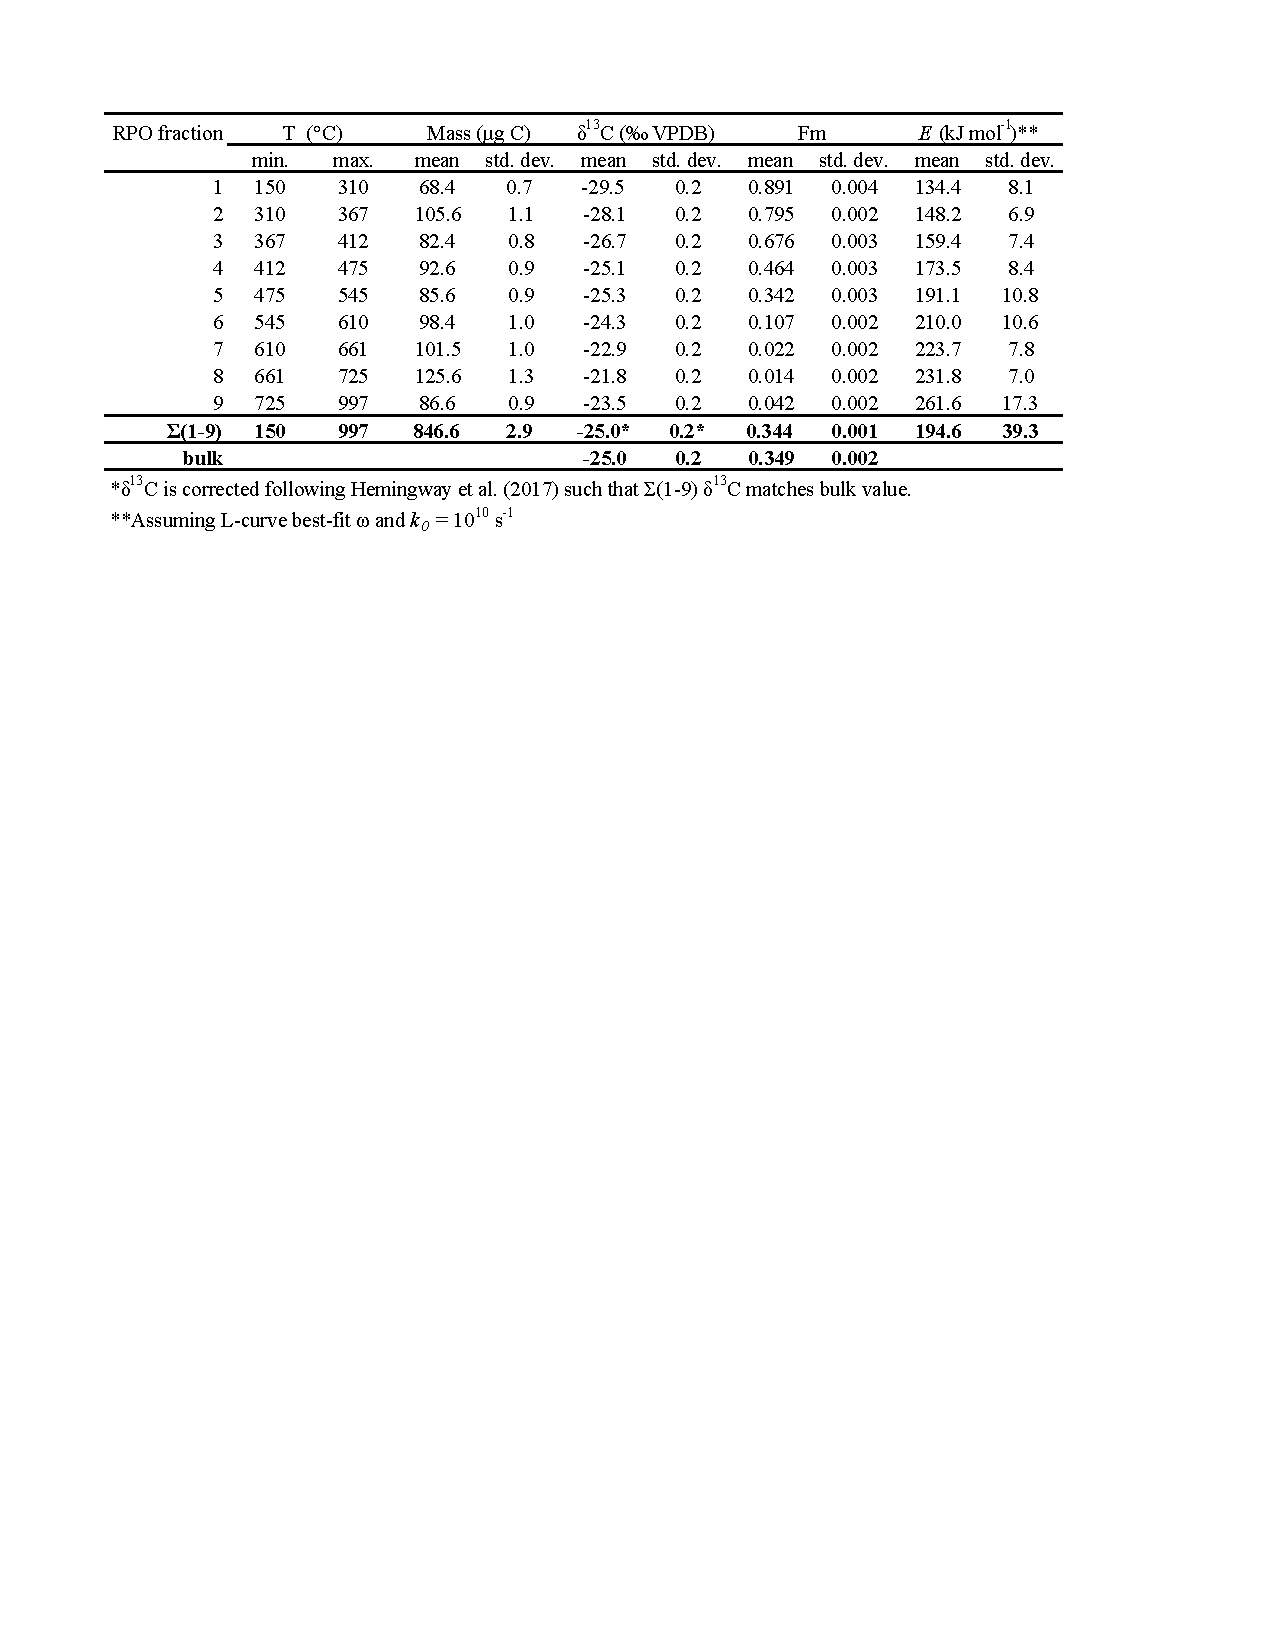
\includegraphics{Thesis_Tables/Ch3Tab2}
	\label{Ch3Tab:2} 
\end{sidewaystable}

% Table 3
\begin{sidewaystable}[p]
	\caption[JGOFS MC-1 RPO results]{JGOFS MC-1 measured RPO temperature ranges, \ce{CO2} masses, \ce{\delta^{13}C}, and modeled $E$ values for each fraction. Also included are mass-weighted averages [$\Sigma(1-5)$] and the independently measured bulk \ce{\delta^{13}C} value.}
	\centering
		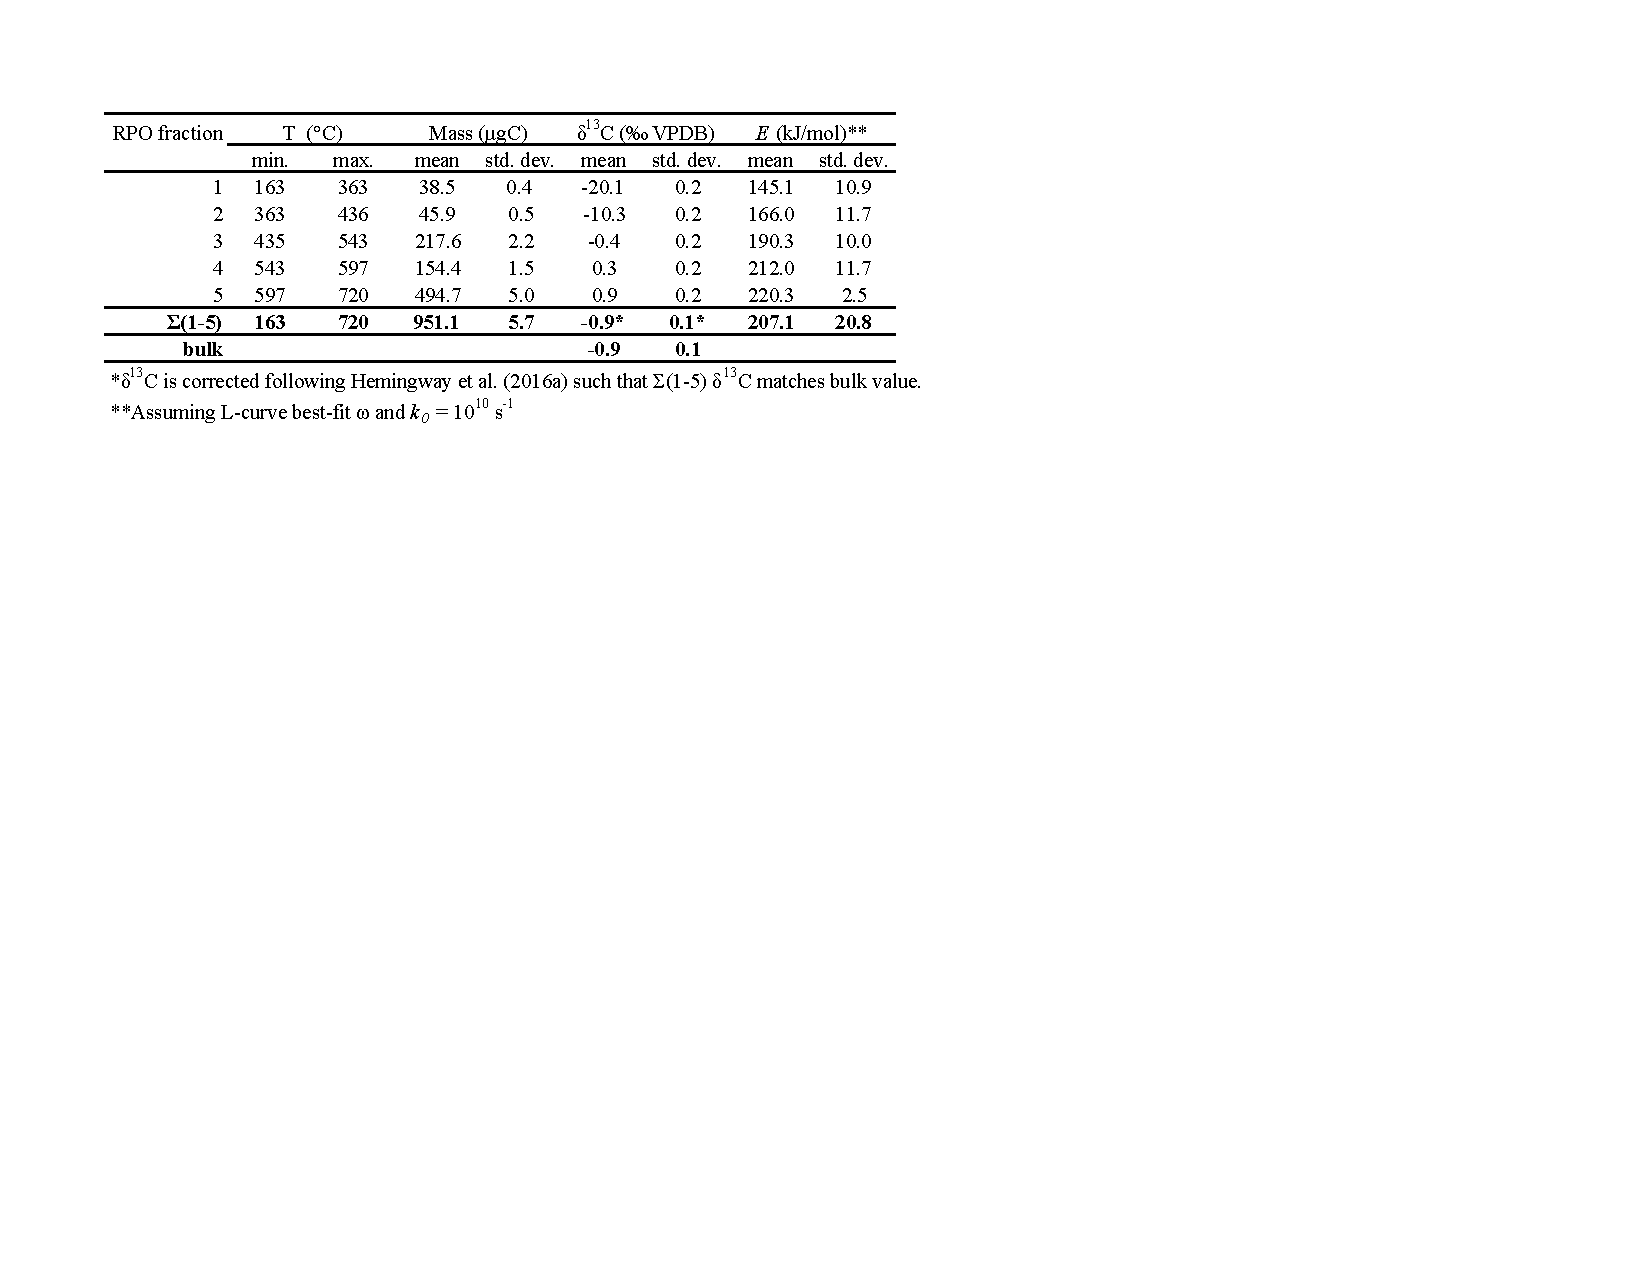
\includegraphics{Thesis_Tables/Ch3Tab3}
	\label{Ch3Tab:3} 
\end{sidewaystable}

% Table 4
\begin{sidewaystable}[p]
	\caption[Pololu 4169 RPO results]{Pololu 4169 measured RPO temperature ranges, \ce{CO2} masses, \ce{\delta^{13}C}, Fm, and modeled $E$ values for each fraction. Also included are mass-weighted averages [$\Sigma(1-5)$] and independently measured bulk isotope values.}
	\centering
		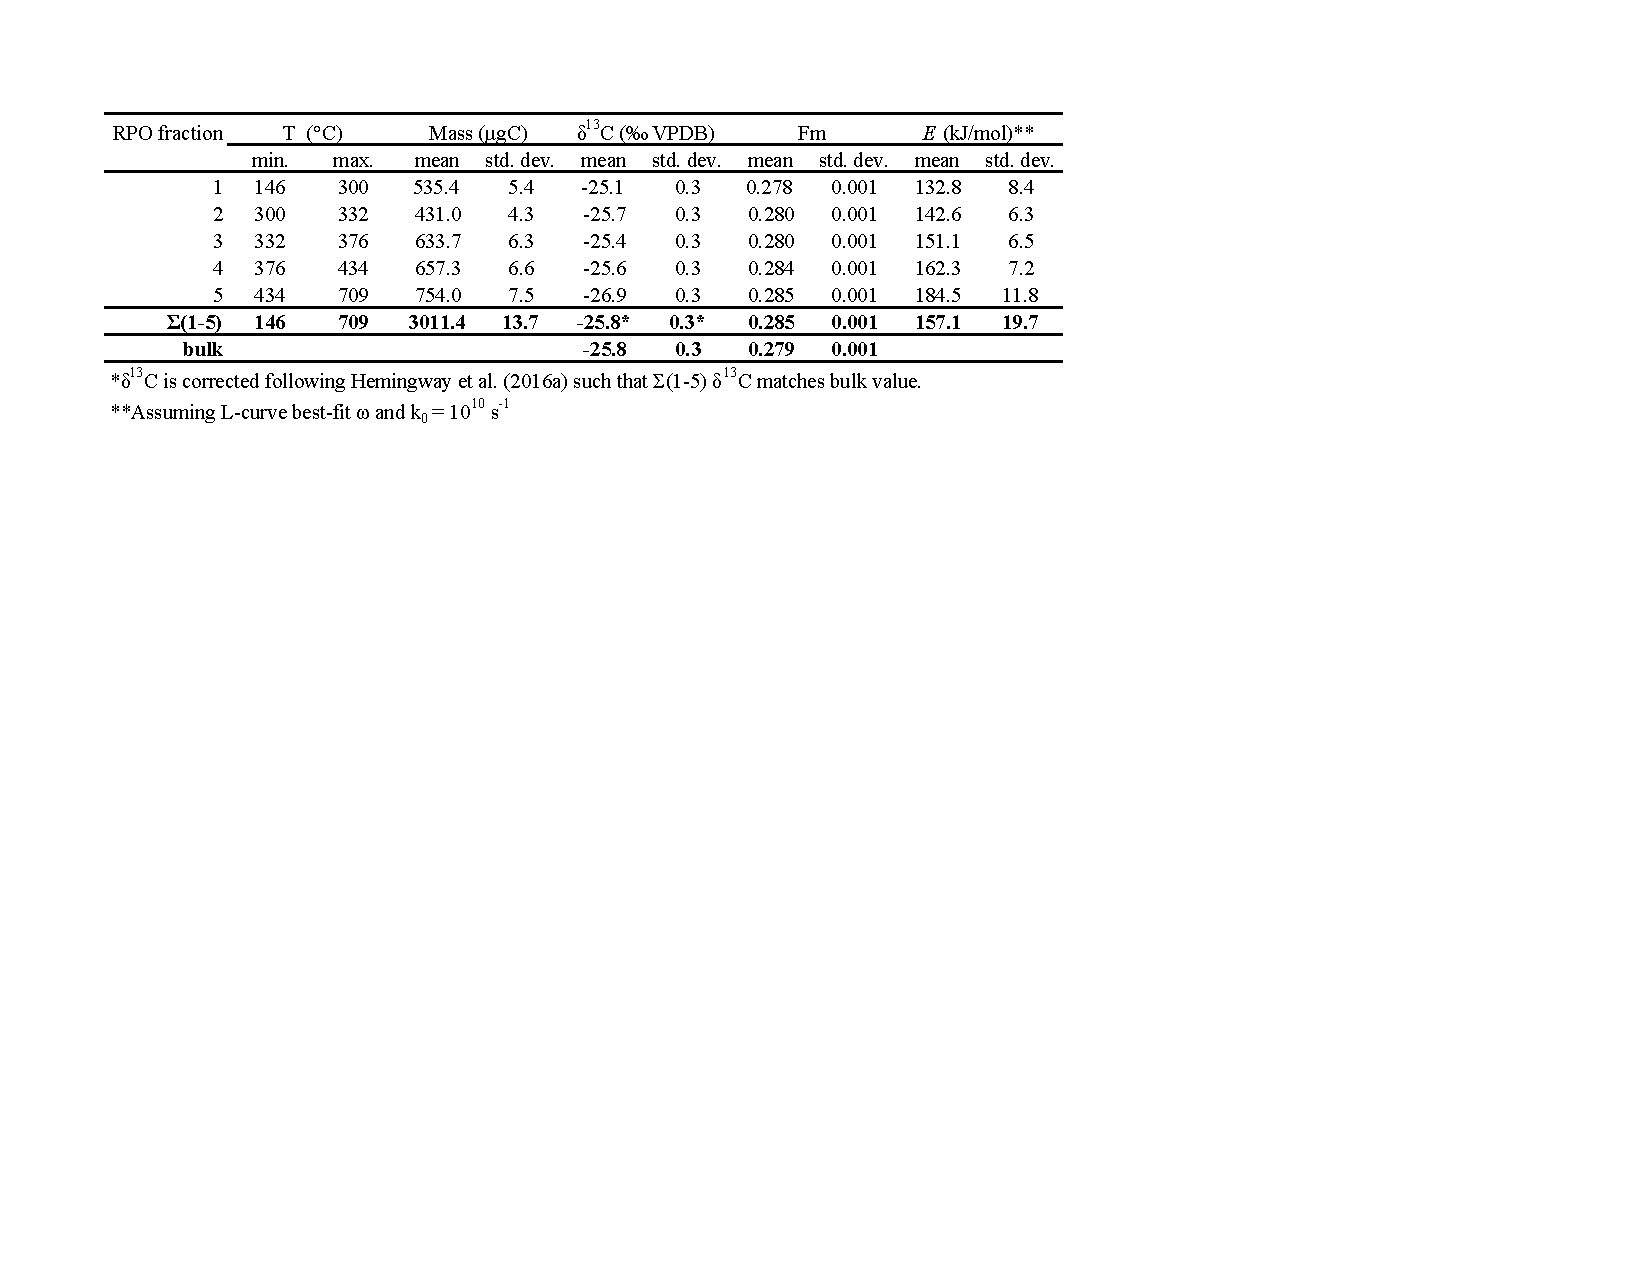
\includegraphics{Thesis_Tables/Ch3Tab4}
	\label{Ch3Tab:4} 
\end{sidewaystable}

In contrast, the JGOFS MC-1 thermogram is dominated by a single peak with a maximum decay rate at \SI{652}{\celsius} (Figure \ref{Ch3Fig:2}B). This is within the range of previously observed carbonate decomposition temperatures \citep{Plante:2013tu}, consistent with the fact that \SI{\approx 95}{\%} of the carbon in this sample is present as calcite \citep{Sayles:2001ua}. While Fm was not measured, \ce{\delta^{13}C} values increase drastically throughout the experiment from \SI{-20.1 \pm 0.2}{\permil.VPDB} (fraction 1) to \SI{0.9 \pm 0.2}{\permil.VPDB} (fraction 5). Lastly, carbon contained in Pololu 4169 exhibits the lowest degradation temperatures of all samples studied, with a maximum decay rate at \SI{348}{\celsius} and \SI{<0.5}{\%} of initial carbon remaining unreacted at \SI{600}{\celsius} (Figure \ref{Ch3Fig:2}C). Fm values are remarkably stable across RPO fractions, ranging from \num{0.278 \pm 0.001} (fraction 1) to \num{0.285 \pm 0.001} (fraction 5). Despite this, \ce{\delta^{13}C} values display a significant decrease with increasing temperature, ranging from \SI{-25.1 \pm 0.3}{\permil.VPDB} (fraction 1) to \SI{-26.9 \pm 0.3}{\permil.VPDB} (fraction 5). 

% Figure 2
\begin{figure}[p]
	\makebox[\textwidth][c]{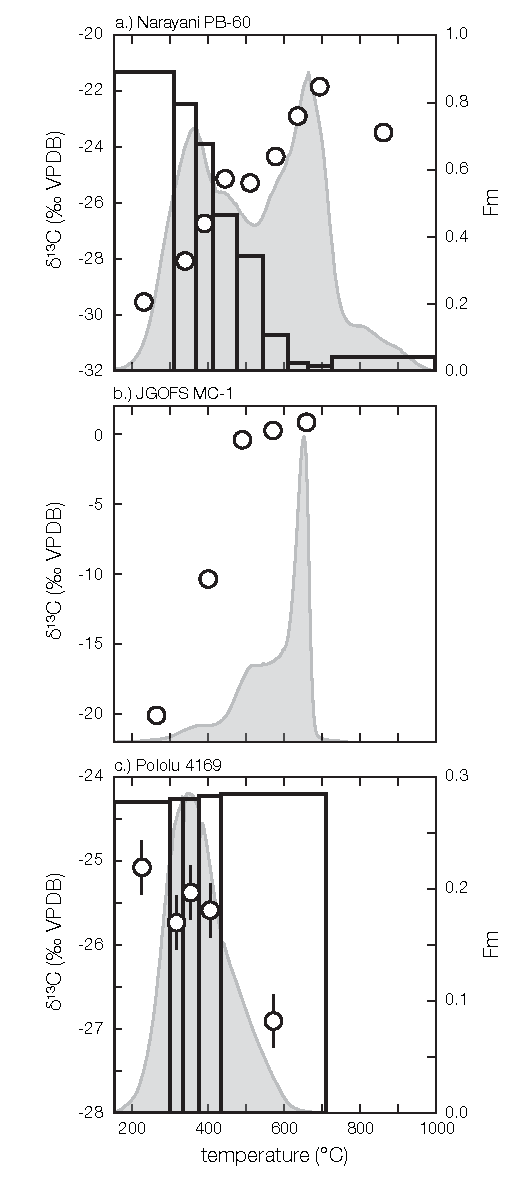
\includegraphics[]{Thesis_Figures/Ch3Fig2}}
	\caption[RPO thermograms, \ce{\delta^{13}C}, and Fm values for all samples]{RPO mass-normalized thermograms (gray shaded region, unitless), \ce{\delta^{13}C} values (white circles, left axis), and Fm values (transparent bars, right axis) for \textit{(A)} Narayani PB-60, \textit{(B)} JGOFS MC-1 (Fm not measured), and \textit{(C)} Pololu 4169. Width of Fm bars corresponds to the temperature range of collection for each RPO fraction. Where visible, \ce{\delta^{13}C} error bars represent propagated analytical uncertainty (Fm uncertainty not visible).}
	\label{Ch3Fig:2} 
\end{figure}

To test if thermogram shapes depend on initial carbon mass ($G_0$), we reanalyzed Nayarani PB-60 and JGOFS MC-1 for various values of $G_0$ while holding all other experimental conditions constant (\textit{i.e.} $\beta = 5$ \si{\celsius.min^{-1}}). Narayani PB-60 thermograms scale linearly with $G_0$ throughout the experiment, with maximum decay rates ranging from \SI{\approx 0.06}{\micro g.C.s^{-1}} ($G_0 = 268$ \si{\micro g.C}) to \SI{\approx 0.20}{\micro g.C.s^{-1}} ($G_0 = 828$ \si{\micro g.C}; Figure \ref{Ch3Fig:3}A). $G_0$ has no apparent effect on elution temperature for this sample, with maximum decay rates observed at \SI{662.0 \pm 0.8}{\celsius} for all values of $G_0$. Similarly, JGOFS MC-1 decay rates scale positively with $G_0$, with a maximum decay rate ranging from \SI{\approx 0.10}{\micro g.C.s^{-1}} ($G_0 = 98$ \si{\micro g.C}) to \SI{\approx 0.88}{\micro g.C.s^{-1}} ($G_0 = 951$ \si{\micro g.C}; Figure \ref{Ch3Fig:3}B). However, unlike Narayani PB-60, the temperature at which maximum decay rates are observed increases with $G_0$ from \SI{620.5}{\celsius} ($G_0 = 98$ \si{\micro g.C}) to \SI{652.2}{\celsius} ($G_0 = 951$ \si{\micro g.C}).

Lastly, we analyzed Narayani PB-60 at multiple ramp rates ($\beta$ = \SIlist{2;5;10}{\celsius.min^{-1}}) while holding $G_0$ constant. Here we normalize thermograms by initial mass and ramp rate in order to accurately compare between experimental conditions, resulting in plots of fractional carbon loss per \si{\celsius} (Figure \ref{Ch3Fig:3}C). Results indicate a consistent shift toward higher elution temperatures for higher ramp rates, as predicted by parallel first-order kinetics \citep{Braun:1987vf,Miura:1995uo,Miura:1998jf}. For example, the temperature at which the maximum decay rate is reached increases from \SI{621.2}{\celsius} when $\beta = 2$ \si{\celsius.min^{-1}} to \SI{688.5}{\celsius} when $\beta = 10$ \si{\celsius.min^{-1}}. This temperature increase is accompanied by a corresponding decrease in decay rate, with maximum values dropping from \SI{3.1e-3}{\celsius^{-1}} ($\beta = 2$ \si{\celsius.min^{-1}}) to \SI{2.7e-3}{\celsius^{-1}} ($\beta = 10$ \si{\celsius.min^{-1}}).

% Figure 3
\begin{figure}[p]
	\makebox[\textwidth][c]{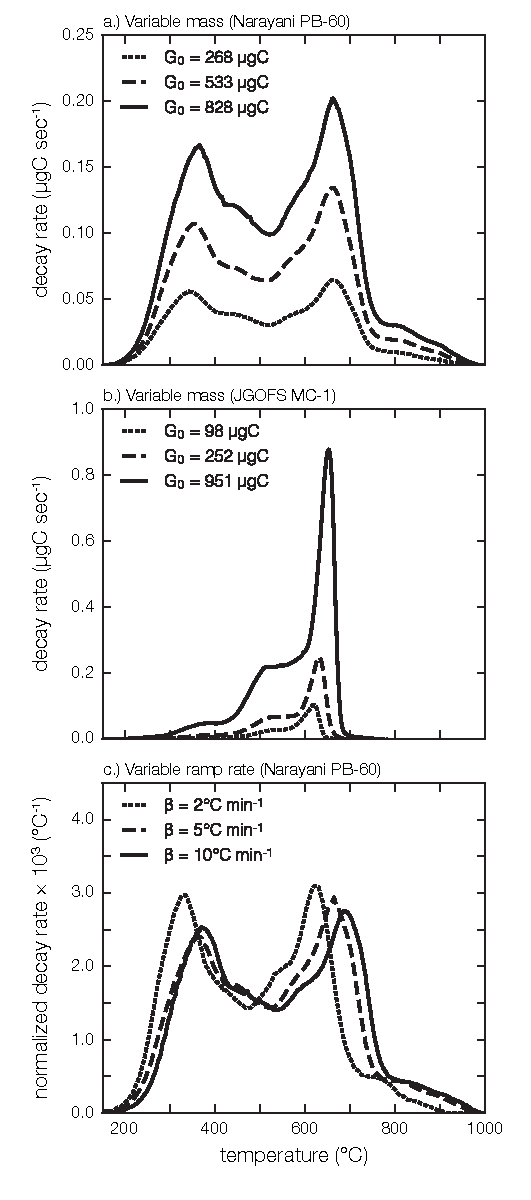
\includegraphics[]{Thesis_Figures/Ch3Fig3}}
	\caption[The effects of initial mass ($G_{0}$) and ramp-rate ($\beta$) on RPO thermograms]{Testing the effects of initial mass ($G_{0}$) and ramp-rate ($\beta$) on RPO thermograms: \textit{(A)} Narayani PB-60 and \textit{(B)} JGOFS MC-1 analyzed for multiple $G_{0}$ values,  \textit{(C)} Narayani PB-60 analyzed for multiple $\beta$ values. Decay rates in panel \textit{(C)} are normalized by $G_{0}$ and $\beta$ in order to properly compare between each analysis.}
	\label{Ch3Fig:3} 
\end{figure}

\section{Discussion}

To properly interpret RPO thermograms as a function of OC chemical composition, and to relate these results with corresponding \ce{\delta^{13}C} and Fm values, remineralization kinetics during thermal degradation must be fully constrained. The distributed activation energy model (DAEM) is a promising method to do so, as it has long been utilized to describe the non-isothermal decay of complex carbon mixtures such as biomass \citep[\textit{e.g.}][]{Bradbury:1979to,White:2011iz} and fossil fuel precursor OC \citep[\textit{e.g.}][]{Burnham:1987ut,Braun:1987vf,Burnham:1999ec,Cramer:2004tg,Dieckmann:2005dw} during thermogravimetric analysis. Here we derive the DAEM  by first considering the case where OC is separated into a finite set of discrete components with unique activation energy values. We then generalize this description to allow for a continuous distribution of OC quality, as has been done previously \citep[see][for review]{Burnham:1999ec}. Finally, following \citet{Forney:2012dr,Forney:2012hz}, we describe an inverse method to determine the regularized solution of the ill-posed DAEM, and compare resulting reaction energetics with RPO fraction \ce{\delta^{13}C} and Fm values.

\subsection{Mathematical derivation}

\subsubsection{Discrete DAEM}

First, we consider the case where OC is described by a finite set of discrete components associated with unique activation energy values. During OC remineralization, the decay rate of carbon contained in a particular component $i$ is often described as as a first-order process with respect to the mass of carbon remaining in component $i$ at any time $t$, $g_{i}(t)$ \citep{Berner:1980ux,Braun:1987vf}:
%
% Equation 1
\begin{equation}\label{Ch3Eq:1}
	\frac{dg_{i}(t)}{dt} = - k_{i}(t) g_{i}(t)
\end{equation}
%
where $k_{i}(t)$ is the dynamic first-order rate coefficient associated with component $i$ at time $t$. Although OC decay in the environment can additionally depend on oxidant concentration, we omit this dependency here since \ce{O2} is provided in excess in our experimental setup. In contrast to the "multi-G" and "reactive continuum" models that are often used to describe environmental OC degradation rates \citep{Westrich:1984uj,Boudreau:1991wf,Forney:2012dr,Forney:2012hz}, here we explicitly allow $k_{i}(t)$ to vary with time. Because rate coefficients are related to temperature and activation energy, $k_{i}(t)$ can be determined as a function of $E$ following the Arrhenius equation so long as temperature is known at each time point:
%
% Equation 2
\begin{equation}\label{Ch3Eq:2}
	k_{i}(t) = k_{0} \exp \left[ - \frac{E_{i}}{RT(t)} \right]
\end{equation}
%
where $k_0$ is the empirically derived Arrhenius pre-exponential ("frequency") factor, $R$ is the ideal gas constant, $E_{i}$ is the activation energy of carbon contained in component $i$, and $T(t)$ is the measured temperature of the system at time $t$. For non-isothermal systems, time-dependent (\textit{i.e.} dynamic) decay coefficients can therefore be described by the static property $E_{i}$ and the observed variable $T(t)$. Although $T(t)$ is related to $t$ by a constant ramp rate $\beta$ during RPO analysis, we leave this written as is to emphasize that the DAEM is valid for any measured time-temperature history. Substituting Equation \ref{Ch3Eq:2} for $k_{i}(t)$, first-order decay during a non-isothermal process at time $t$ can be written as:
%
% Equation 3
\begin{equation}\label{Ch3Eq:3}
	\frac{dg_{i}(t)}{dt} = - k_{0} \exp \left[ - \frac{E_{i}}{RT(t)} \right] g_{i}(t)
\end{equation}
%
The mass of carbon remaining in component $i$ at time $t$ is therefore determined by integrating Equation \ref{Ch3Eq:3} from an initial time, $t_{0} = 0$, to a final time $t$:
%
% Equation 4
\begin{equation}\label{Ch3Eq:4}
	g_{i}(t) = g_{i,0} \exp \left[ - k_{0} \int_{0}^{t} \exp \left\{ - \frac{E_{i}}{RT(t')} \right\} dt' \right]
\end{equation}
%
where $g_{i,0}$ is the initial mass of carbon contained in component $i$ and $t'$ is the change-of-variables substituted time variable ranging from $t_{0} = 0$ to $t$. Due to the integration of the Arrhenius equation from $t_{0} = 0$ to $t$, Equation \ref{Ch3Eq:4} states that $g_{i}(t)$ depends on the entire time-temperature history of the experiment. That is, $\frac{dg_{i}(t)}{dt}$ is governed by a balance between decreasing $g_{i}(t)$ as OC is remineralized and increasing $k_{i}(t)$ with increasing $T(t)$ as the experiment progresses. This balance should result in a predictable shift in RPO thermograms toward higher elution temperatures with increasing $\beta$, as is observed \citep[Figure \ref{Ch3Fig:3}C;][]{Braun:1987vf,Miura:1995uo,Miura:1998jf}.

Furthermore, following the multi-G model of \citet{Westrich:1984uj}, any environmental sample containing a complex OC mixture can be described as a superposition of a finite set of $n$ components, each decaying according to a unique $k_{i}(t)$ and thus corresponding to a unique $E_{i}$ value. The total carbon mass remaining at $t$, $G(t)$, is therefore the sum of the mass remaining in each component $i = 1,2,\dots,n$ at that time:
%
% Equation 5
\begin{equation}\label{Ch3Eq:5}
	\begin{split}
		G(t) & = \sum_{i=1}^{n} g_{i}(t) \\
		& =  G_{0} \sum_{i=1}^{n} p_{i,0} \exp \left[ - k_{0} \int_{0}^{t} \exp \left\{ - \frac{E_{i}}{RT(t')} \right\} dt' \right]
	\end{split}
\end{equation}
%
where $G_{0}$ is the initial OC mass present in the entire sample, defined as the sum of initial mass contained in each component:
%
% Equation 6
\begin{equation}\label{Ch3Eq:6}
	G_{0} = \sum_{i=1}^{n} g_{i,0}
\end{equation}
%
and $p_{i,0}$ is the fraction of total carbon initially contained in component $i$:
%
% Equation 7
\begin{equation}\label{Ch3Eq:7}
	p_{i,0} = \frac{g_{i,0}}{G_{0}}
\end{equation}
%
such that $\sum_{i=1}^{n} p_{i,0} \equiv 1.0$. The fraction of OC initially present within each component can therefore be determined by fitting Equation \ref{Ch3Eq:5} to the observed $G(t)$ profile measured by the RPO instrument. While informative, this discrete description of the DAEM suffers from two major limitations: \textit{(i)} $n$ must be set \textit{a priori} or determined empirically \citep{Boudreau:1991wf} and \textit{(ii)} any noise recorded in the data will result in large uncertainty in best-fit $p_{i,0}$ and $E_{i}$ values \citep{Forney:2012hz}. To circumvent these issues, a more general description of non-isothermal first-order decay can be derived that does not assume a finite set of components with unique $E_{i}$, but rather allows $E$ to vary continuously \citep{Burnham:1987ut,Burnham:1999ec,Cramer:2004tg}.

\subsubsection{Continuous DAEM}

In this continuous model, the mass of carbon remaining at time $t$ that is associated with any activation energy value $E$, $g(t, E)$, can be determined by substituting $g(t,E)$ for $g_{i}(t)$ and $E$ for $E_{i}$ in Equation \ref{Ch3Eq:4}:
%
% Equation 8
\begin{equation}\label{Ch3Eq:8}
	g(t, E) = g_{0}(E) \exp \left[ - k_{0} \int_{0}^{t} \exp \left\{ - \frac{E}{RT(t')} \right\} dt' \right]
\end{equation}
%
where $g_{0}(E)$ is the initial mass of carbon associated with activation energy value $E$. The total carbon mass remaining at time $t$, $G(t)$, can now be defined by replacing the summation over components $i = 1,2,\dots,n$ in Equation \ref{Ch3Eq:5} by an integral over all possible (\textit{i.e.} non-negative) values of $E$:
%
% Equation 9
\begin{equation}\label{Ch3Eq:9}
	\begin{split}
	G(t) & = G_{0} \int_{0}^{\infty} p_{0}(E) \\
	& \qquad\qquad \exp \left[ - k_{0} \int_{0}^{t} \exp \left\{ - \frac{E}{RT(t')} \right\} dt' \right] dE
	\end{split}
\end{equation}
%
where $p_{0}(E) dE$ is now the fraction of total carbon initially associated with the infinitesimal range of activation energy values about $E$ such that:
%
% Equation 10
\begin{equation}\label{Ch3Eq:10}
    \int_{0}^{\infty} p_{0}(E) dE  \equiv 1
\end{equation}
%
That is, the distribution of $p_{0}(E)$ over all values of $E$ describes the initial probability density function (pdf) of activation energy that will lead to the observed OC decay rates when a sample is analyzed in the RPO instrument. Unlike measured thermograms, $p_{0}(E)$ is not a function of experimental conditions such as ramp rate -- rather, it is an intrinsic property of the physical-chemical bonding environment within a particular sample. As RPO analysis proceeds, this pdf must evolve with time to reflect the fact that some carbon has been remineralized to \ce{CO2}. Therefore, at any time $t$ the remaining fraction of total OC initially present in the sample that is associated with any activation energy value, $p(t, E) dE$, is calculated as $p_{0}(E)dE$ multiplied by a double exponential decay term analogous to Equation \ref{Ch3Eq:8}:
%
% Equation 11
\begin{equation}\label{Ch3Eq:11}
	p(t,E) dE = p_{0}(E) \exp \left[ - k_{0} \int_{0}^{t} \exp \left\{ - \frac{E}{RT(t')} \right\} dt' \right] dE
\end{equation}
%
Equation \ref{Ch3Eq:11} implies that the carbon initially remineralized to \ce{CO2} must be associated with the lowest values of $E$, as low $E$ will lead to a double exponential term that approaches zero most rapidly. Put differently, OC that is described by higher $E$ values will resist remineralization until more time has passed and, therefore, higher temperatures have been reached -- \textit{i.e.} it is more thermally recalcitrant.

\subsection{Verification of parallel first-order kinetics}

Because the DAEM is a specific case of \textit{n}-order non-isothermal kinetic models \citep{Braun:1987vf,White:2011iz}, we must verify that carbon degradation in the RPO instrument behaves according to a superposition of parallel first-order reactions (with respect to OC concentration) rather than higher-order processes. Differentiating Equation \ref{Ch3Eq:9} with respect to time, the total rate of carbon remineralization at any time $t$ is given by the equation:
%
% Equation 12
\begin{equation} \label{Ch3Eq:12}
	\begin{split}
	\frac{dG(t)}{dt}  & = - G_{0} \int_{0}^{\infty} p_{0}(E) k_{0} \exp \left[ - \frac{E}{RT(t)} \right] \\
		& \qquad\qquad \exp \left[ - k_{0} \int_{0}^{t} \exp \left\{ - \frac{E}{RT(t')} \right\} dt' \right] dE \\
	& = - G_{0} \int_{0}^{\infty} p(t, E) k_{0} \exp \left[ - \frac{E}{RT(t)} \right] dE \\
	\end{split}
\end{equation}
%
It can be seen that the DAEM describes $\frac{dG(t)}{dt}$ as a linear function of $G_{0}$ multiplied by an integral term that depends on $p(t,E)$ but is independent of $G_{0}$. In contrast, if carbon decomposition within the RPO instrument were to follow a higher-order process, the relationship between $\frac{dG(t)}{dt}$ and $G_{0}$ would be nonlinear and evolve as a function of time \citep[\textit{e.g.}][]{Follett:2014if}. Replacing the integral term in Equation \ref{Ch3Eq:12} by $m(t)$, the loss of carbon at time $t$ as predicted by the DAEM simplifies to:
%
% Equation 13
\begin{equation} \label{Ch3Eq:13}
	\frac{dG(t)}{dt} = - G_{0} m(t)
\end{equation}
%
Therefore, similar to the isothermal case described in \citet{Follett:2014if}, a superposition of parallel first-order decay reactions will result in a linear relationship between $\frac{dG(t)}{dt}$ and $G_{0}$ with a zero intercept and a time-dependent slope equal to:
%
% Equation 14
\begin{equation}\label{Ch3Eq:14}
 	m(t) = \int_{0}^{\infty} p(t, E) k_{0} \exp \left[ - \frac{E}{RT(t)} \right] dE
\end{equation}
%
where $m(t)$ can be interpreted as the $G_{0}$-normalized decay rate at time $t$. We verify that OC remineralization within the RPO instrument follows parallel first-order kinetics by assessing the linearity between $\frac{dG(t)}{dt}$ and $G_{0}$ at any time $t$ across a range of $G_{0}$ values using Narayani PB-60 a test sample (Figure \ref{Ch3Fig:3}A). We chose Narayani PB-60 because it exhibits the widest range of decomposition temperatures of any sample analyzed here (Figure \ref{Ch3Fig:2}). For 4 arbitrarily chosen time points, it can be seen that this relationship is linear with an ordinary least squares $R^{2} \geq 0.999$ (Figure \ref{Ch3Fig:4}A), resulting in identical $G_{0}$-normalized thermograms within analytical uncertainty (Figure \ref{Ch3Fig:4}B). Therefore, the decay of complex OC mixtures contained in decarbonated samples during RPO analysis can indeed be accurately described by a superposition of parallel first-order reactions.

% Figure 4
\begin{figure}[p]
	\makebox[\textwidth][c]{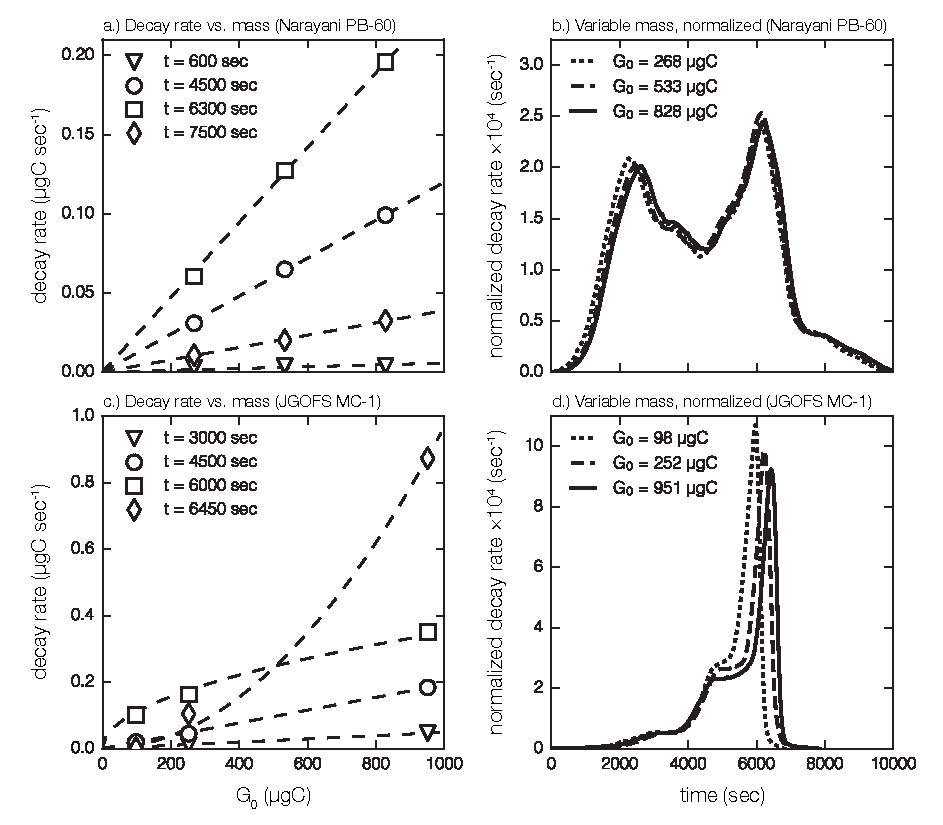
\includegraphics[]{Thesis_Figures/Ch3Fig4}}
	\caption[Assessment of first-order kinetics]{First-order kinetic assessment: \textit{(A)} decay rate vs. $G_{0}$ relationships at four arbitrarily chosen time points for Narayani PB-60, including best-fit regressions (dashed lines); \textit{(B)} mass-normalized decay rates for each analysis used in \textit{(A)}; \textit{(C)} decay rate vs. $G_{0}$ relationships at four arbitrarily chosen time points for JGOFS MC-1, including best-fit regressions (dashed lines); and \textit{(D)} mass-normalized decay rates for each analysis used in \textit{(C)}. Linear relationships and nearly identical normalized decay rates in panels \textit{(A)--(B)} confirm the first-order nature of OC decay, while non-linear relationships and a shifting carbonate peak in panels \textit{(C)--(D)} indicate non-first-order \ce{CaCO3} decay kinetics.}
	\label{Ch3Fig:4} 
\end{figure}

\subsubsection{A note of caution for carbonates}\label{Ch3Sec:3521}

While most RPO studies to date have focused on OC analysis by acidifying to remove carbonates \citep[\textit{e.g.}][]{Rosenheim:2008ed,Rosenheim:2012kh,Rosenheim:2013dka,Schreiner:2014jr,Bianchi:2015jr}, it has recently been argued that acid hydrolysis and/or dissolution of short range order minerals during acid treatment can alter the OC chemical bonding environment and therefore affect thermal stability \citep{Plante:2013tu}. Analyzing raw samples without acid treatment can circumvent these issues, however the effect of carbonates on decay kinetics has not yet been considered. To test if carbonate-rich samples follow parallel first-order kinetics, we similarly analyzed JGOFS MC-1 for a range of $G_{0}$ values (Figure \ref{Ch3Fig:3}B). Prior to $t \approx 4500$ s, when \ce{\delta^{13}C} values of eluted \ce{CO2} indicate a predominantly OC source (Figure \ref{Ch3Fig:2}B), $\frac{dG(t)}{dt}$ can be accurately described as a linear function of $G_{0}$ ($R^{2} \geq 0.999$). However, as carbonate begins to decompose above $t \approx 4500$ s, the relationship between $\frac{dG(t)}{dt}$ and $G_{0}$ becomes highly nonlinear -- that is, the resulting carbonate peak shifts toward higher $t$ with increasing $G_{0}$ (Figure \ref{Ch3Fig:4}C--D). 

To investigate if non-first-order decomposition is an intrinsic property of \ce{CaCO3} or if this is due to interactions with other materials within the sample (so-called "matrix effects"), we additionally analyzed a purified Icelandic spar \ce{CaCO3} standard at multiple masses ($G_{0}$ = \SIlist{258;492;1014}{\micro g.C}, $\beta$ = \SI{5}{\celsius.min^{-1}}). Results indicate that purified carbonate, unlike JGOFS MC-1, does follow first-order kinetics, with a maximum decomposition rate occurring at \SI{700 \pm 6}{\celsius} independent of $G_{0}$ (not shown). Interaction with reduced organic carbon, corresponding hetero-atoms (\textit{e.g.} N, P, S), or trace metals contained within the sample matrix are therefore the likely cause of non-first-order \ce{CaCO3} decomposition when analyzing environmental samples. Thus, while avoiding the issues of acid treatment, the analysis of carbonate-containing samples will result in thermograms that cannot be accurately described by the DAEM presented here, and is not recommended when using the RPO instrument to determine reaction energetics.


\subsection{Solving for $p_{0}(E)$ using an inverse method}

Following \citet{Forney:2012dr,Forney:2012hz}, we present a method to invert the DAEM and solve for the pdf of $E$ subject to a non-negativity constraint. In contrast to previous DAEM solutions \citep{Lakshmanan:1994vs,Cai:2007hh,deCaprariis:2012jk}, this approach does not require an \textit{a priori} assumption about the parametric form of $p_{0}(E)$. Additionally, because inverse methods are ill-posed and thus highly sensitive to noise, we "smooth" the solution using a Tikhonov regularization to remove this sensitivity \citep{Tikhonov:1977ui,Hansen:1994uc}. To numerically calculate $p_{0}(E)$, we discretize the continuous variable $t$ over the time course of the experiment into a vector $\mathbf{t}$ containing $n_{t}$ nodes, $t_{j}$, such that:
%
% Equation 15
\begin{equation}\label{Ch3Eq:15}
	\Delta t_{j} = \frac{1}{2} \left(t_{j} - t_{j-1} \right) + \frac{1}{2} \left(t_{j+1} - t_{j} \right)
\end{equation}
%
For generality, and because the DAEM is frequently applied over geologic timescales with non-uniformly distributed time measurements, Equation \ref{Ch3Eq:15} does not require a uniform time step (\textit{i.e.} it is possible that $\Delta t_{j} \neq \Delta t_{i \neq j}$). Similarly, we generate a vector $\mathbf{E}$ over the range values considered for the model solution (typically \SIrange{50}{350}{kJ.mol^{-1}}) that contains $n_{E}$ nodes, $E_{l}$, such that:
%
% Equation 16
\begin{equation}\label{Ch3Eq:16}
	\Delta E_{l} = \frac{1}{2} \left(E_{l} - E_{l-1} \right) + \frac{1}{2} \left(E_{l+1} - E_{l} \right)
\end{equation}
%
It can be seen from Equation \ref{Ch3Eq:9} that the DAEM can be separated into two components: \textit{(i)} $p_{0}(E)$ and \textit{(ii)} a double exponential term that is independent of $p_{0}(E)$. This term, analogous to the Laplace transform for the isothermal reactive continuum model \citep{Forney:2012hz}, describes the fraction of carbon initially associated with an activation energy value $E$ that has decayed by time $t$. We therefore generate a matrix $\mathbf{A}$ describing the dynamic disordered kinetics of the system by calculating the value of this term for all combinations of $t_{j}$ and $E_{l}$:
%
% Equation 17
\begin{equation}\label{Ch3Eq:17}
	A_{j,l} = \exp \left\{ -\sum_{u=0}^{j} k_{0} \exp \left[ - \frac{E_{l}}{RT(t_{u})} \right] \Delta t_{u} \right\} \Delta E_{l}
\end{equation}
%
Finally, we integrate the measured RPO thermogram and interpolate the resulting fraction of total carbon remaining at each time point, $\frac{G(t)}{G_{0}}$, onto each discretized time point in $\mathbf{t}$ to generate a vector of fractional carbon remaining, $\mathbf{g}$. The DAEM can thus be written in matrix form as:
%
% Equation 18
\begin{equation}\label{Ch3Eq:18}
	\mathbf{g} = \mathbf{A} \cdot \mathbf{p}
\end{equation}
%
where $\mathbf{p}$ is a discretized vector of $p_{0}(E)$ with length $n_{l}$ such that each component $p_{l}$ is equal to:
%
% Equation 19
\begin{equation}\label{Ch3Eq:19}
	p_{l} = \frac{1}{\Delta E_{l}} \int_{ \frac{1}{2} \left(E_{l} + E_{l-1} \right)}^{\frac{1}{2} \left(E_{l} + E_{l+1} \right)} p_{0}(E) dE
\end{equation}
%
While $\mathbf{p}$ can be calculated directly by multiplying $\mathbf{g}$ by the computed inverse of $\mathbf{A}$, it is possible that this will result in negative values of $p_{l}$ if $\mathbf{g}$ contains noisy data \citep{Forney:2012hz}. However, because $p_{l}$ represents a probability, it cannot be negative by definition. We therefore require the solution to be non-negative by solving the constrained least squares problem according to:
%
% Equation 20
\begin{equation}\label{Ch3Eq:20}
	\min_{\mathbf{p}} \| \mathbf{A} \cdot \mathbf{p} - \mathbf{g} \|^{2}
\end{equation}
%
where $\| \mathbf{x} \| \equiv \sqrt{ \sum x_{i}^{2}}$ is the vector norm and we require that $p_{l} \geq 0$. The resulting $\mathbf{p}$ vector is thus the non-regularized solution to the inverse DAEM.

\subsubsection{Choice of frequency factor}

In order to construct the $\mathbf{A}$ matrix and solve for $\mathbf{p}$, our method requires that the Arrhenius pre-exponential factor $k_{0}$ be prescribed \textit{a priori}. There exists significant discussion in the literature on the best choice of $k_{0}$, as multiple values of this parameter can describe laboratory results equally well but will result in drastically different predictions of OC degradation rates over geologic timescales \citep{Braun:1987vf,Burnham:1987ut,Lakshmanan:1991tr,Dieckmann:2005dw}. Furthermore, it has been argued that $k_{0}$ represents the variable change in entropy associated with the decay of specific organic compounds and should therefore be parameterized as a function of $E$ \citep[the so-called "kinetic compensation effect" or "KCE";][]{Tang:2000ua}. For example, a linear increase in $k_{0}$ with $E$ from \SI{\approx e8}{s.^{-1}} ($E$ = \SI{175}{kJ.mol^{-1}}) to \SI{\approx e26}{s^{-1}} ($E$ = \SI{400}{kJ.mol^{-1}}) has been utilized to better predict petroleum formation rates \citep{Dieckmann:2005dw}. To circumvent the issue of multiplicity, and to account for the KCE, \citet{Miura:1995uo} and \citet{Miura:1998jf} developed a method to estimate the best-fit $k_{0}$ for each value of $E$ by comparing the shift in elution temperatures when a sample is analyzed at multiple ramp rates (\textit{e.g.} Figure \ref{Ch3Fig:3}C). However, because this approach is based on large extrapolations in $\frac{1}{T}$ vs. $\frac{\beta}{T^{2}}$ space, it is highly sensitive to noise in temperature and $\beta$ measurements \citep{Burnham:1989vm}.

To select a best-fit $k_{0}$, here we calculate $\mathbf{A}$ and $\mathbf{p}$ for a range of $k_{0}$ values and determine the root mean squared error (RMSE) between measured $G(t)$ and that predicted by Equation \ref{Ch3Eq:20}. We include the KCE by calculating $k_{0}$ as a function of $E$ according to:
%
% Equation 21
\begin{equation}\label{Ch3Eq:21}
	\log_{10} k_{0} = (\text{KCE slope})E + (\text{KCE intercept})
\end{equation}
%
Resulting RMSE values using a range of KCE slope and intercept can be seen in Figure \ref{Ch3Fig:5} for Narayani PB-60 ($\beta$ = \SI{5}{\celsius.min^{-1}}, $E$ ranging from \SIrange{50}{350}{kJ.mol^{-1}}). By setting an "acceptable" cutoff of RMSE \num{\leq e-4}, it can be seen that there exist multiple KCE slope and intercept combinations that can equally fit the observed data. Additionally, we estimate the best-fit $k_{0}$ using a range of ramp rates ($\beta$ = \SIlist{2;5;10}{\celsius.min^{-1}}) following the method of \citet{Miura:1998jf} (Figure \ref{Ch3Fig:5}, white circle). While this estimate falls outside of the RMSE cutoff range, likely due to noise in temperature and $\beta$ measurements, it results in a KCE slope near zero and suggests that $k_{0}$ is constant during RPO oxidation of this sample. To accurately compare RPO results between samples, we therefore select a constant $k_{0}$ value of \SI{e10}{s^{-1}}, well within the RMSE cutoff range, for all samples analyzed herein (Figure \ref{Ch3Fig:5}, red star). While a different choice of $k_{0}$ will shift $p_{0}(E)$ to higher or lower absolute values of $E$, we emphasize that it will not affect the distribution of $p_{0}(E)$, and that only relative changes in $E$ should be interpreted. For example, although a shift in $k_{0}$ from a constant value of \SIrange{e7}{e12}{s^{-1}} results in an increase in mean $E$ from \SIrange{150}{224}{kJ.mol^{-1}} for Narayani PB-60, the resulting relative standard deviation of $p_{0}(E)$ remains identical at \SI{20}{\%}.
 
 % Figure 5
 \begin{figure}[t]
	\makebox[\textwidth][c]{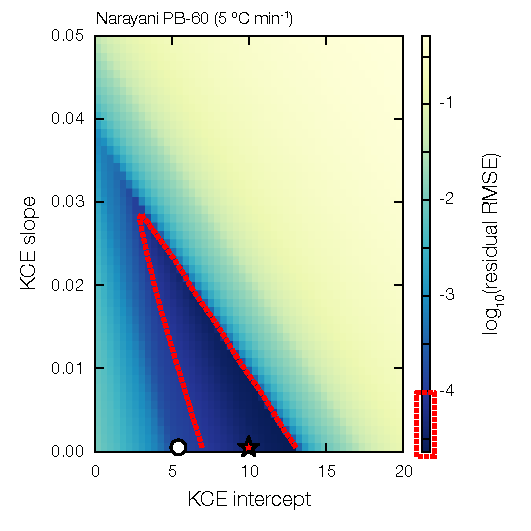
\includegraphics[]{Thesis_Figures/Ch3Fig5}}
	\caption[Residual RMSE using a range of KCE slopes and intercepts for Narayani PB-60]{Model residual RMSE using a range of KCE slopes and intercepts for Narayani PB-60 ($\beta$ = \SI{5}{\celsius.min^{-1}}). Each pixel represents the best-fit result using Equation \ref{Ch3Eq:20} for a given $k_{0}$ as determined by Equation \ref{Ch3Eq:21}. "Acceptable" fits with residual RMSE \num{\leq e-4} are contained within the red dotted line. Estimated result using the method of \citet{Miura:1998jf} for 3 ramp rates ($\beta$ = \SIlist{2;5;10}{\celsius.min^{-1}}) is plotted as a white circle, while the point corresponding to $k_{0}$ = \SI{e10}{\s^{-1}} (the value chosen for all samples in this study) is plotted as a red star.}
	\label{Ch3Fig:5} 
\end{figure}

\subsubsection{Tikhonov Regularization}

In principle, after choosing a value of $k_{0}$ and constructing the $\mathbf{A}$ matrix, the nonparametric pdf of $E$ that best describes an RPO thermogram can be determined using Equation \ref{Ch3Eq:20}. However, the inverse DAEM is highly sensitive to noise at the level of RPO instrument precision \citep[\textit{i.e.} approximately \SI{\pm 5}{ppm.\ce{CO2}}, \SI{\pm 5}{\celsius};][]{Hemingway:2016rc}, and is therefore ill-posed \citep{Hansen:1994uc}. To minimize this sensitivity to data uncertainty, we "smooth" the inverse DAEM solution using Tikhonov regularization \citep{Tikhonov:1977ui,Hansen:1994uc,Forney:2012dr,Forney:2012hz}. This approach is often used to solve constrained inverse problems by calculating an optimal solution that minimizes complexity in $p_{0}(E)$ (as determined by the intensity of fluctuations, or "roughness") while maximizing solution accuracy. Following \citet{Forney:2012hz}, we calculate roughness as the norm of the first derivative of $\mathbf{p}$:
%
% Equation 22
\begin{equation}\label{Ch3Eq:22}
	\left\| \frac{d p_{0}(E)}{dE} \right\| = \sqrt{ \sum_{l=1}^{n_{l}}\left( \frac{p_{l+1} - p_{l}}{E_{l+1} - E_{l}}\right)^{2}} = \| \mathbf{R} \cdot \mathbf{p} \| 
\end{equation}
%
where $\mathbf{R}$ is the discretized first derivative operator over the range of $E$ values considered. The regularized inverse solution can therefore be determined by including this roughness term when solving the constrained least squares:
%
% Equation 23
\begin{equation}\label{Ch3Eq:23}
	\min_{\mathbf{p}} \| \mathbf{A} \cdot \mathbf{p} - \mathbf{g} \|^{2} + \omega \| \mathbf{R} \cdot \mathbf{p} \|^{2}
\end{equation}
%
where $\omega$ is a scalar that determines how much to weight the roughness relative to the residual error. The best choice of $\omega$ is often considered to be the value that optimally minimizes the residual error and solution roughness. As described in \citet{Hansen:1994uc}, this is equal to the value corresponding to the point of maximum curvature in a $\log-\log$ plot of the residual error vs. the roughness when allowing $\omega$ to range over many orders of magnitude (\textit{i.e.} the so-called "L-curve", Figure \ref{Ch3Fig:6}). The best-fit $\omega$ value as determined by the L-curve therefore results in a "smoothed" solution of $p_{0}(E)$ with a residual error that is, in principle, approximately equal to the measurement uncertainty \citep{Forney:2012hz}. 

% Figure 6
\begin{figure}[p]
	\makebox[\textwidth][c]{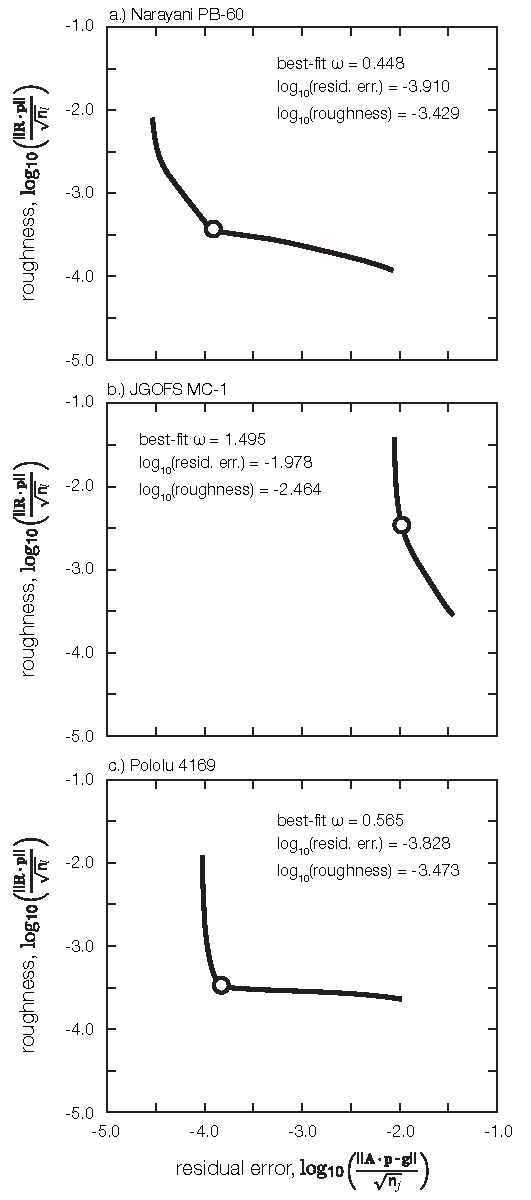
\includegraphics[]{Thesis_Figures/Ch3Fig6}}
	\caption[Tikhonov Regularization L-curves for all samples analyzed]{Tikhonov Regularization L-curves for all samples analyzed ($\beta$ = \SI{5}{\celsius.min^{-1}}): \textit{(A)} Narayani PB-60, \textit{(B)} JGOFS MC-1, and \textit{(C)} Pololu 4169. White circle corresponds to the point of maximum curvature -- \textit{i.e.} the best-fit $\omega$ value. Note the $\approx 100 \times$ higher residual error for JGOFS MC-1 due to the presence of carbonates.}
	\label{Ch3Fig:6} 
\end{figure}

However, we note that the best-fit residual error for JGOFS MC-1 is $\approx 100$-fold higher than for Narayani PB-60 and Pololu 4169 due to the non-first-order decay of \ce{CaCO3} that cannot be accurately predicted by the DAEM, as described above (Section \ref{Ch3Sec:3521}, Figure \ref{Ch3Fig:6}B). This results in a $G_{0}$-dependent $p_{0}(E)$ distribution, with the resulting $E$ value associated with the carbonate peak in this sample shifting from \SI{211}{kJ.mol^{-1}} when $G_{0}$ = \SI{98}{\micro g.C} to \SI{220}{kJ.mol^{-1}} when $G_{0}$ = \SI{951}{\micro g.C} (not shown). Still, regularized pdfs of $E$ for samples containing exclusively OC are nearly identical across all experimental conditions (\textit{i.e.} $\beta$, $G_{0}$), supporting the hypothesis that $p_{0}(E)$ is an intrinsic property of OC contained within a sample. For example, although there exist small differences between individual runs due to measurement uncertainty and variability in best-fit $\omega$ values (range of \numrange{0.044}{0.448}, $n=5$), the main features of the pdf of $E$ contained within Narayani PB-60 are robust for all conditions considered in this study (Figure \ref{Ch3Fig:7}). 

% Figure 7
\begin{figure}[t]
	\makebox[\textwidth][c]{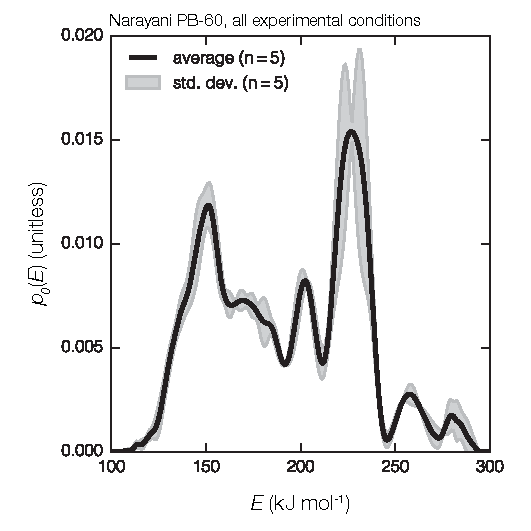
\includegraphics[]{Thesis_Figures/Ch3Fig7}}
	\caption[Average Narayani PB-60 $p_{0}(E)$ distribution for all experimental conditions]{Mean (black line) and standard deviation (gray shaded region) of regularized $p_{0}(E)$ distributions for Narayani PB-60 analyzed using a range of $G_{0}$ and $\beta$ values ($n = 5$), indicating that DAEM results are largely independent of experimental conditions for decarbonated samples.}
	\label{Ch3Fig:7} 
\end{figure}

Unlike previous studies that assume a Gaussian distribution of $p_{0}(E)$ during fossil fuel pyrolysis \citep{Lakshmanan:1994vs,Cai:2007hh,deCaprariis:2012jk}, regularized results calculated here clearly do not follow any parametric form (Figure \ref{Ch3Fig:8}, thick black lines). Rather, it can be seen that $p_{0}(E)$ generally resembles the RPO thermogram shape (Figure \ref{Ch3Fig:2}), as would be expected due to the fact that thermally recalcitrant OC is associated with higher values of $E$. Furthermore, observed high-frequency variability in $p_{0}(E)$ relative to the corresponding thermograms is an intrinsic result of non-isothermal kinetics. That is, during RPO analysis, OC associated with a single $E$ value will decompose over a range of temperatures with an increasing rate coefficient until it has been exhausted, thus resulting in a "smoothed" thermogram relative to the governing $p_{0}(E)$ distribution. Highly variable, non-parametric $p_{0}(E)$ observed here likely results from the extreme chemical complexity and  range of oxidation states contained in environmental OC samples \citep[\textit{e.g.}][]{Kellerman:2015jn}. In contrast, fossil fuel precursors have undergone various degrees of diagenesis and thermal maturation, potentially resulting in OC mixtures exhibiting more similar chemical properties that can be described by a Gaussian distribution of pyrolysis $E$ values \citep{Braun:1987vf}. This proposed relationship between $p_{0}(E)$ complexity and chemical diversity is additionally supported by the differences between samples analyzed herein. For example, fluvial suspended sediments such as Narayani PB-60 integrate a range of OC sources \citep[\textit{e.g.} recently fixed biomass, pre-aged soils, and eroded rock-derived material;][]{Blair:2012du} and would therefore be expected to contain a broader and more variable $p_{0}(E)$ distribution than that contained in a single soil OC sample such as Pololu 4169, as is observed (Table \ref{Ch3Tab:2}, \ref{Ch3Tab:4}; Figure \ref{Ch3Fig:8}A, \ref{Ch3Fig:8}C). We therefore propose that variability in the pdf of $E$ is a useful metric for comparing relative OC chemical complexity between samples.

% Figure 8
\begin{figure}[p]
	\makebox[\textwidth][c]{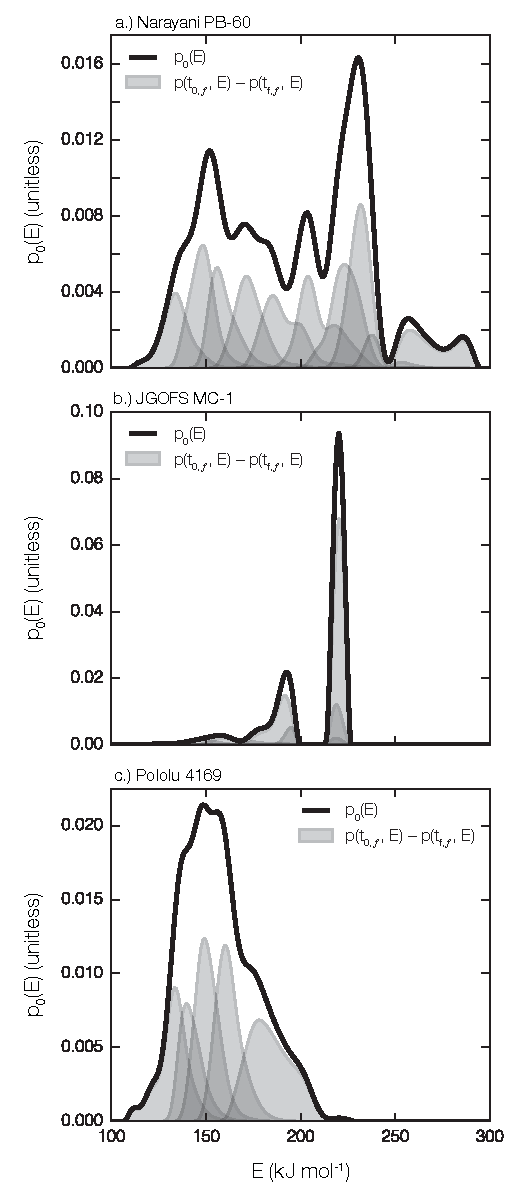
\includegraphics[]{Thesis_Figures/Ch3Fig8}}
	\caption[$p_{0}(E)$ distributions for all RPO fractions in all samples]{Regularized $p_{0}(E)$ distributions (black line) and the corresponding subset of $p_{0}(E)$ that is contained in each RPO fraction (gray shaded region): \textit{(A)} Narayani PB-60, \textit{(B)} JGOFS MC-1, and \textit{(C)} Pololu 4169. Overlapping distributions are a result of the fact that OC described by a single $E$ value decays over a range of temperatures.}
	\label{Ch3Fig:8} 
\end{figure}

\subsubsection{Determining $\bm{p_{0}(E)}$ contained in each RPO fraction}

To further understand how the distribution of OC molecular structure relates with source and reservoir age, we compare the average $E$ value corresponding to \ce{CO2} contained within each RPO fraction with its corresponding isotope composition. To do so, we first calculate the subset of the pdf of $E$ that is contained within an RPO fraction $f$ by taking the difference between $p(t,E)$ at the initial and final time points for each fraction. Because $A_{j,l}$ describes the relative amount of carbon initially associated with $E_{l}$ remaining at time $t_{j}$, it can be seen from Equation \ref{Ch3Eq:11} that the discretized $p(t_{j},E)$ values can be calculated by multiplying each $p_{l}$ in $\mathbf{p}$ by the corresponding element in the $j^{\text{th}}$ row of $\mathbf{A}$. The pdf of $E$ corresponding to the \ce{CO2} contained in each RPO fraction is therefore equal to $p(t_{\text{0},f},E) - p(t_{\text{f},f},E)$ for each value of $E$, where $t_{\text{0},f}$ and $t_{\text{f},f}$ are the initial and final time points, respectively, for RPO fraction $f$. Resulting distributions are typically non-parametric and highly overlapping, reflecting the fact that \ce{CO2} isotope composition for each RPO fraction is itself a weighted average of multiple sources (Figure \ref{Ch3Fig:8}, gray shaded regions). Average $E$ values and corresponding variance can thus be calculated as the first and second moments, respectively, of each distribution (Table \ref{Ch3Tab:2}--\ref{Ch3Tab:4}).

\subsection{Relationships between isotopes and reaction energetics}

\subsubsection{Kinetic isotope fractionation}

While not necessary for Fm because it is fractionation-corrected by definition \citep{Stuiver:1977uh,dosSantos:2007ca}, we must correct for any kinetic isotope effects occurring within the RPO instrument before interpreting \ce{\delta^{13}C} as a carbon source tracer \citep{Hemingway:2016rc}. If kinetic fractionation is large, as has been observed both during thermogenic methane formation \citep{Tang:2000ua,Cramer:2004tg} and dissolved OC oxidation by \textit{uv} light \citep{Oba:2008fv}, then this effect could overprint carbon source \ce{\delta^{13}C} signals. However, when directly measured using single-compound standards, \citet{Hemingway:2016rc} concluded that \ce{^{13}C} fractionation within the RPO instrument must be smaller than \SIrange{\approx 1}{\approx 2}{\permil}. Still, we correct the measured \ce{\delta^{13}C} values of each RPO fraction using the ratio of carbon-normalized \ce{^{13}C} and \ce{^{12}C} decomposition rates at each time point:
%
% Equation 24
\begin{equation}\label{Ch3Eq:24}
	\ce{^{13/12}r}(t) = \frac{\left( \frac{d \ce{^{13}}G(t)}{dt} \right)}{\left( \frac{d \ce{^{12}G}(t)}{dt} \right)} \left( \frac{\ce{^{12}G}_0}{\ce{^{13}G}_0} \right)
\end{equation}
%
Where we have added a preceding $12$ or $13$ superscript to specify isotope-specific variables. Following the Arrhenius equation, $\ce{^{13/12}r}(t)$ can be described as a function of the difference in $E$ between \ce{^{13}C}- and \ce{^{12}C}-containing molecules:
%
% Equation 25
\begin{equation}\label{Ch3Eq:25}
	\ce{^{13-12}\Delta E} = \ce{^{13}E} - \ce{^{12}E}
\end{equation}
%
Although \ce{^{13-12}\Delta E} is likely not identical for all compounds due to differences in the entropy and enthalpy of isotope substitution \citep{Tang:2000ua}, the estimated range of values for RPO analysis is small \citep[\SIrange{0.3e-3}{1.8e-3}{kJ.mol^{-1}};][]{Hemingway:2016rc}. We therefore assume \ce{^{13-12}\Delta E} = \SI{1.8e-3}{kJ.mol^{-1}} for all RPO fractions, noting that a choice of \SI{0.3e-3}{kJ.mol^{-1}} would result in \ce{\delta^{13}C} values that are identical to those calculated here within analytical uncertainty.

$\ce{^{13/12}r}(t)$ can be determined using the ratio of carbon-normalized, isotope-specific decay rates as calculated in Equation \ref{Ch3Eq:12} by substituting $p_{0}(\ce{^{12}E})$ and $p_{0}(\ce{^{13}E})$ for $p_{0}(E)$. Because carbon is present as \SI{\approx 99}{\%} \ce{^{12}C}, we set $p_{0}(\ce{^{12}E}) = p_{0}(E)$ such that $\frac{d \ce{^{12}G}(t)}{dt} = \frac{dG(t)}{dt}$. Corresponding $\frac{d \ce{^{13}G}(t)}{dt}$ can then be determined using $p_{0}(\ce{^{13}E}) = p_{0}(E + \ce{^{13-12}\Delta E})$. That is, \ce{^{13}C}-containing molecules decay at rates governed by a pdf of $E$ that is identical to $p_{0}(E)$ but has been shifted to the right by \SI{1.8e-3}{kJ.mol^{-1}}. We then correct the measured \ce{\delta^{13}C} values of each RPO fraction $f$ for kinetic isotope fractionation by dividing by the average $\ce{^{13/12}r}(t)$ value over the time of collection [written as $\mean{\ce{^{13/12}r}(t)_{f}}$]:
%
% Equation 26
\begin{equation}\label{Ch3Eq:26}
	\ce{\delta^{13}C}_{f, \text{corrected}} = \frac{1}{\mean{\ce{^{13/12}r}(t)_{f}}} \left( \ce{\delta^{13}C}_{f} + 1000 \left[ \mean{\ce{^{13/12}r}(t)_{f}} - 1 \right] \right)
\end{equation}
%
For the samples analyzed here,  $\ce{^{13/12}r}(t)$ is initially \num{\approx 0.999}, indicating slightly faster decay of \ce{^{12}C} at low temperatures, and gradually increases to \num{\approx 1.002} when $G(t) \ll 0.01 G_{0}$,  as has been described previously \citep{Cramer:2004tg,Hemingway:2016rc}. Resulting kinetic fractionation corrections are near or within analytical uncertainty, with absolute \ce{\delta^{13}C} values for all RPO fractions shifted by \SI{< 0.2}{\permil} ($\ce{\delta^{13}C}_{f, \text{corrected}} - \ce{\delta^{13}C}_{f}$: maximum = \SI{+0.16}{\permil}, Pololu 4169 fraction 1; minimum = \SI{-0.10}{\permil}, Narayani PB-60 fraction 9).

\subsubsection{Comparing $\bm{p_{0}(E)}$, \ce{^{13}C} content, and \ce{^{14}C} content}

In addition to exhibiting the narrowest and least complex pdf of $E$, Pololu 4169 displays a much smaller spread in both \ce{\delta^{13}C} and Fm values than does Narayani PB-60 (Figure \ref{Ch3Fig:9}A--D), supporting the idea that highly complex $p_{0}(E)$ distributions reflect the integration of multiple OC sources with variable chemical structures and reservoir ages. Pololu 4169 Fm values are low and stable for all RPO fractions (Figure \ref{Ch3Fig:9}B), indicating that low-$E$ OC can become significantly pre-aged given the proper environmental conditions \citep{Schmidt:2011gg}. Furthermore, Fm values for this sample display a small yet statistically significant increase with increasing $E$, opposite of what would be expected if thermal recalcitrance were a major driver of reservoir age (\SI{0.0001}{[kJ.mol^{-1}]^{-1}}, $R^{2} = 0.895$, $p$-value = \num{1.5e-2}). Coincident with increasing Fm, \ce{\delta^{13}C} decreases slightly with increasing $E$ (Figure \ref{Ch3Fig:9}A), suggesting a second source of \ce{^{13}C}-depleted, \ce{^{14}C}-enriched OC at higher $E$ values, potentially due to downward percolation of surface dissolved OC \citep{Chadwick:2007hc}. Still, the fact that Fm does not decrease with increasing $E$ is consistent with the current paradigm of soil carbon dynamics, which interprets reservoir age as an ecosystem property rather than a function of OC chemical structure \citep{Mikutta:2006gx,Janssens:2010hd,Schmidt:2011gg}. 

Pololu 4160 $p_{0}(E)$ distribution is concentrated at low $E$ values and is dominated by a large, broad peak despite the fact that soil OC contains a mixture of humic material, lipids, carbohydrates, lignin, \textit{etc.} \citep[Figure \ref{Ch3Fig:8}C;][]{Helfrich:2007ej}. RPO analysis therefore does not result in a separation of complex OC mixtures into individual, highly resolved peaks representing individual compounds or compound classes. Combined with a relatively homogenous \ce{\delta^{13}C} and Fm values between RPO fractions, a narrow $p_{0}(E)$ distribution indicates that individual compound classes contained in environmental samples are not separable based on thermal lability despite the unique decomposition temperatures when analyzed as purified compounds \citep{Williams:2014bq}. In contrast, it is well known that individual biomarkers such as lignin and \textit{n}-alkanoic acids contained in soils can display drastically different \ce{^{14}C} content \citep[see][for review]{Schmidt:2011gg}. The fact that this is not observed between RPO fractions is strong evidence that OC decomposing at any given $E$ value does not correspond to a single compound or simple set of compounds, but is rather derived from a mix of sources. This can be achieved, for example, if relatively oxidized functional groups decompose at low $E$ independent of their chemical source, while the remaining aromatic and aliphatic core structures resist degradation until higher temperatures have been reached. This interpretation indicates that RPO analysis separates OC based on the redox state and bonding environment of individual carbon atoms rather than properties of whole molecules, analogous to the process by which enzymes degrade OC in the environment \citep{Sinsabaugh:2008il}. 

% Figure 9
\begin{figure}[p]
	\makebox[\textwidth][c]{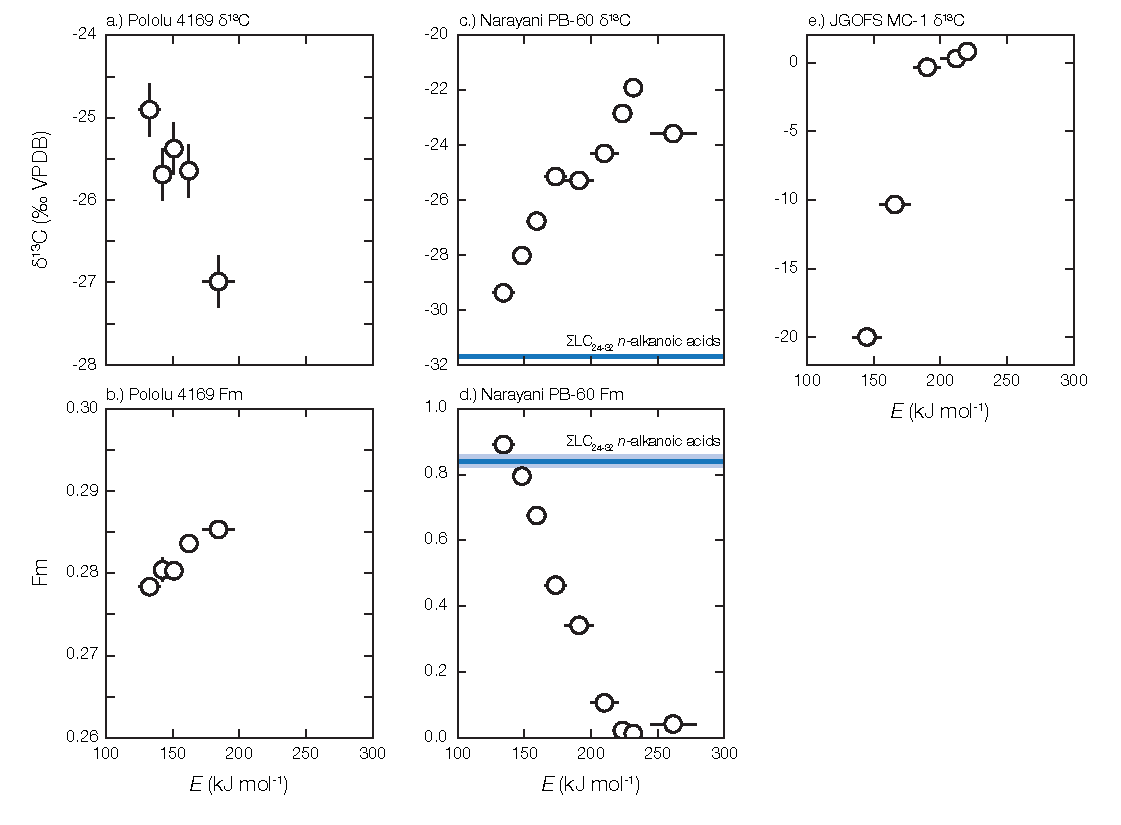
\includegraphics[]{Thesis_Figures/Ch3Fig9}}
	\caption[RPO $E$ vs. isotope plots for all fractions in all samples]{Plots of resulting $E$ vs. fractionation-corrected \ce{\delta^{13}C} or Fm for each sample analyzed: Pololu 4169 [\textit{(A)} \ce{\delta^{13}C}, \textit{(B)} Fm], Narayani PB-60 [\textit{(C)} \ce{\delta^{13}C}, \textit{(D)} Fm], and JGOFS MC-1 [\textit{(E)} \ce{\delta^{13}C}]. Error bars in \ce{\delta^{13}C} and Fm represent propagated analytical uncertainty, while error bars in $E$ are the standard deviation contained within each fraction. Blue lines in panel \textit{(C)} and \textit{(D)} are the $\Sigma$LC\sub{24--32} \textit{n}-alkanoic acid \ce{\delta^{13}C} and Fm values, with shaded regions representing the reported $\pm 1 \sigma$ uncertainty \citep{Galy:2011hk,Galy:2011ix}.}
	\label{Ch3Fig:9} 
\end{figure}

Still, significant trends in isotope composition with increasing $E$ can be observed. For example, the relationship between \ce{\delta^{13}C} and $E$ for Narayani PB-60 RPO fractions 1 through 8 is remarkably linear, with a slope of \SI{0.07}{\permil.(kJ.mol^{-1})^{-1}} ($R^{2} = 0.954$, $p$-value = \num{3.2e-5}; Figure \ref{Ch3Fig:9}C). The \SI{\approx 4}{\permil} \ce{^{13}C} depletion in fraction 9 relative to what would be expected based on this trend is at least partially due to charring, as has been described previously during non-isothermal OC pyrolysis \citep{Williams:2014bq}. Charring can result in an apparent shift toward higher $E$ values for labile OC compounds, as free-radical formation and subsequent condensation of aromatic material will increase thermal stability. However, because it has been shown that processes occurring in series can still be treated as a superposition of parallel reactions \citep{Forney:2014ws}, charring does not violate the kinetic model developed here. Rather, this simply results in a small inclusion of otherwise labile OC within the highest-temperature RPO fraction.

Nonetheless, fractions 1 through 8 strongly suggest that Narayani PB-60 OC contains 2 end members that mix linearly as a function of $E$. Importantly, although the isotope composition of \ce{CO2} contained in each RPO fraction represents a weighted average of OC associated with a particular $E$ range, this does not inherently require a linear mixing trend between fractions. For example, mixing two theoretical end members with identical $p_{0}(E)$ distributions but contrasting \ce{^{13}C} compositions will shift each RPO fraction along the \ce{\delta^{13}C} axis (\textit{i.e.} vertically in Figure \ref{Ch3Fig:9}C) according to the relative contribution of each end member, resulting in a "flat" \ce{\delta^{13}C} relationship with $E$. In contrast, a mixture of two end members containing drastically different chemical structures and thus non-overlapping $p_{0}(E)$ distributions would lead to two "clusters" of points in a plot of \ce{\delta^{13}C} vs. $E$. A linear trend like that observed here therefore indicates two end members with unique \ce{^{13}C} compositions yet complex, overlapping $p_{0}(E)$ distributions. That is, it requires a decrease in the contribution by a \ce{^{13}C}-depleted end member and a corresponding increase in the contribution by a \ce{^{13}C}-enriched end-member with increasing $E$. 

This is further evidenced by the similarly linear trend in Fm with increasing $E$ for RPO fractions 1 through 8 (slope = \SI{-0.01}{[kJ.mol^{-1}]^{-1}}, $R^{2} = 0.987$, $p$-value = \num{7.6e-7}). Unlike Pololu 4169, \SI{\approx 20 \pm 5}{\%} of OC contained in Narayani PB-60 is derived from the erosion of OC-rich bedrock in this catchment \citep[OC\sub{petro};][]{Galy:2008ff,Rosenheim:2012kh}. Because this material is \ce{^{14}C}-free by definition, and because it has been shown that similarly condensed "black" carbon pyrolyses above \SI{\approx 650}{\celsius} \citep{Williams:2014bq}, OC\sub{petro} is the likeliest source of high-$E$ OC in this sample. However, strong linear trends in both \ce{\delta^{13}C} and Fm with increasing $E$ require that a fraction of this material has been incorporated into lower $E$ OC, as the pyrolysis temperatures observed in \citet{Williams:2014bq} correspond to an $E$ value greater than \SI{\approx 200}{kJ.mol^{-1}}. Similar to the observation in Pololu 4169 that biospheric OC (OC\sub{bio}) generally contains low $E$ values, previously measured \ce{\delta^{13}C} and Fm values of long-chain \textit{n}-alkanoic acids extracted from Narayani PB-60 are consistent with the lowest $E$ RPO fractions \citep[Figure \ref{Ch3Fig:9}C--D;][]{Galy:2011hk,Galy:2011ix}. 

Therefore, a binary mixture combining biospheric OC\sub{bio} described by relatively homogenous Fm near that of \textit{n}-alkanoic acids and an $E$ distribution similar to Pololu 4169 with unaltered OC\sub{petro} described by $E \geq 200$ \si{kJ.mol^{-1}} would result in "clustered" RPO fractions in Figure \ref{Ch3Fig:9}D due to the lack of significant $E$ overlap. This is clearly not observed. Rather, the linear trends observed for both \ce{\delta^{13}C} vs. $E$ and Fm vs. $E$ require the presence of two end members with unique isotope compositions but overlapping $p_{0}(E)$. This further indicates that each "peak" in a distribution of $p_{0}(E)$ (\textit{e.g.} Figure \ref{Ch3Fig:8}A) does not represent an isotopically unique signal derived from a specific class of compounds. Instead, this implies that each end-member contains carbon atoms described by similar chemical bonding environments and redox states. RPO analysis is therefore ideally suited for separating isotopically unique yet chemically overlapping OC sources.

Lastly, we note that JGOFS MC-1 RPO \ce{\delta^{13}C} values are driven by a sharp increase in \ce{CaCO3} contribution at higher $E$ values, with fraction 5 matching the independently measured calcite value \citep[Figure \ref{Ch3Fig:9}E;][]{Sayles:2001ua}. Although carbon in this sample is present as \SI{\approx 95}{\%} calcite, the \ce{\delta^{13}C} value of fraction 1 is near that expected for phytoplankton biomass OC in this region \citep{Rau:1989wr}, suggesting that RPO analysis can sufficiently separate low-$E$ OC from \ce{CaCO3} despite the potential for catalysis, matrix effects, and non-first-order kinetics. Still, we emphasize that non-first-order kinetics and mass-dependent \ce{CaCO3} elution temperatures do hinder our ability to interpret changes in OC isotope composition for carbonate-containing samples. We therefore do not recommend quantitatively interpreting RPO isotope and $p_{0}(E)$ results from carbonate-rich samples without independent constraints on end-member composition. 

\section{Conclusion}

Serial oxidation techniques such as RPO are a promising new class of methods for relating OC chemical composition, isotopic composition, and environmental residence times. To better interpret these data, we develop an inverse kinetic model that determines the underlying distribution of activation energy required to thermally degrade OC. Unlike previous implementations of this model, our description does not require any \textit{a priori} assumptions about the shape of the pdf of $E$ values, $p_{0}(E)$, but rather determines the regularized non-parametric solution. By analyzing Narayani PB-60 using a range of oven ramp rates and initial masses, we show that the underlying $E$ distribution is independent of experimental conditions and is therefore an intrinsic property of the OC chemical bonding environment. In contrast, results from a \ce{CaCO3}-rich sample, JGOFS MC-1, indicate that inorganic carbon degradation rates cannot be predicted by our model, likely due to catalytic reactions and matrix effects during RPO analysis.

To compare reaction energetics with measured \ce{\delta^{13}C} and Fm values, we describe the temporal evolution of $p_{0}(E)$ during an RPO experiment and calculate the average $E$ value corresponding to the carbon contained in each fraction. After correcting \ce{\delta^{13}C} values for kinetic isotope fractionation, plots of \ce{\delta^{13}C} vs. $E$ and Fm vs. $E$ indicate that activation energy is strongly correlated with OC isotope composition for the samples analyzed herein. RPO results are consistent with hypothesized controls on OC source and residence time as determined by bulk and compound-specific isotope measurements. We therefore suggest that paired kinetic and isotopic measurements as determined by RPO analysis can offer novel insight into a range of carbon cycle processes.


%\section{Acknowledgements}

%We are grateful to the NOSAMS sample prep lab staff, especially Ann P. McNichol, Mary Lardie-Gaylord, and Alan Gagnon for assistance in running the RPO instrument and measuring isotope results. We thank Carl Johnson (WHOI) for bulk \%OC and \ce{\delta^{13}C} measurements and Katherine Grant (Cornell University) for supplying the RPO results for the Pololu 4169 sample. V.V.G. was partly supported by the US National Science Foundation (grants OCE-0851015 and OCE-0928582), the WHOI Coastal Ocean Institute (grant 27040213) and an Independent Study Award (grant 27005306) from WHOI; J.D.H. was partly supported by the NSF Graduate Research Fellowship Program under grant number 2012126152.


% Chapter 4 text
\chapter{Multiple plant-wax compounds record differential sources and ecosystem structure in large river catchments}
\label{Ch4}
\raggedbottom

{\let\thefootnote\relax\footnotetext{This chapter was originally published as: Hemingway J.D., Schefu\ss \ E., Dinga B.J., Pryer H., and Galy V.V. (2016) {Multiple plant-wax compounds record differential sources and ecosystem structure in large river catchments.} \emph{Geochimica at Cosmochimica Acta}, \textbf{184}, 20--40. Used with permission as granted in the original copyright agreement.}}

\clearpage

\section{Abstract}

The concentrations, distributions, and stable carbon isotopes (\ce{\delta^{13}C}) of plant waxes carried by fluvial suspended sediments contain valuable information about terrestrial ecosystem characteristics. To properly interpret past changes recorded in sedimentary archives it is crucial to understand the sources and variability of exported plant waxes in modern systems on seasonal to inter-annual timescales. To determine such variability, we present concentrations and \ce{\delta^{13}C} compositions of three compound classes (\textit{n}-alkanes, \textit{n}-alcohols, \textit{n}-alkanoic acids) in a 34-month time series of suspended sediments from the outflow of the Congo River.

We show that exported plant-dominated \textit{n}-alkanes (C\textsubscript{25}--C\textsubscript{35}) represent a mixture of C\textsubscript{3} and C\textsubscript{4} end members, each with distinct molecular distributions, as evidenced by an $8.1 \pm  0.7$\textperthousand\ ($\pm1\sigma$ standard deviation) spread in \ce{\delta^{13}C} values across chain-lengths, and weak correlations between individual homologue concentrations ($r = 0.52 - 0.94$). In contrast, plant-dominated \textit{n}-alcohols (C\textsubscript{26}--C\textsubscript{36}) and \textit{n}-alkanoic acids (C\textsubscript{26}--C\textsubscript{36}) exhibit stronger positive correlations ($r = 0.70 - 0.99$) between homologue concentrations and depleted \ce{\delta^{13}C} values (individual homologues average $\leq -31.3$\textperthousand\ and $ -30.8$\textperthousand, respectively), with lower \ce{\delta^{13}C} variability across chain-lengths ($2.6 \pm 0.6$\textperthousand\ and $2.0 \pm 1.1$\textperthousand, respectively). All individual plant-wax lipids show little temporal \ce{\delta^{13}C} variability throughout the time-series ($1\sigma \leq 0.9$\textperthousand), indicating that their stable carbon isotopes are not a sensitive tracer for temporal changes in plant-wax source in the Congo basin on seasonal to inter-annual timescales.

Carbon-normalized concentrations and relative abundances of \textit{n}-alcohols ($19 - 58$\% of total plant-wax lipids) and \textit{n}-alkanoic acids ($26 - 76$\%) respond rapidly to seasonal changes in runoff, indicating that they are mostly derived from a recently entrained local source. In contrast, a lack of correlation with discharge and low, stable relative abundances ($5 - 16$\%) indicate that \textit{n}-alkanes better represent a catchment-integrated signal with minimal response to discharge seasonality. Comparison to published data on other large watersheds indicates that this phenomenon is not limited to the Congo River, and that analysis of multiple plant-wax lipid classes and chain lengths can be used to better resolve local vs. distal ecosystem structure in river catchments.

\section{Introduction}

Since their discovery \citep{Eglinton:1962uj,Eglinton:1967uz}, the information recorded in the composition of aliphatic plant-wax lipids has been utilized extensively as a recorder of terrestrial ecosystem structure both in modern settings \citep{Diefendorf:2011hg,Bush:2013ie} and the geologic past \citep[see][for review]{Pancost:2004ij,Eglinton:2008hs,Freeman:2014gi}. Much attention has been focused on long-chain (\textit{i.e.} greater than $\approx$ 23 carbons) saturated \textit{n}-alkanes, such that the detection of distinct homologue distributions among plant functional types (PFTs) has lead to the use of homologue ratios as a tracer for \textit{n}-alkane sources and ecosystem composition \citep{Ficken:2000wq,Pancost:2002un,Bingham:2010jt}. Such ratios have been frequently utilized in geologic records to infer past ecosystem changes, assuming a straightforward relationship between \textit{n}-alkane production and PFT coverage. However, it has recently been recognized that mixing of \textit{n}-alkanes is likely nonlinear with respect to ecosystem composition, as the absolute production rate of these compounds varies greatly by PFT and between individual species within the same PFT \citep{Rommerskirchen:2006gr,Vogts:2009fb,Diefendorf:2011hg,Bush:2013ie,Magill:2013ab,Garcin:2014hg}. To circumvent these issues, the simultaneous measurement of additional \textit{n}-alkyl lipid classes (\textit{i.e.} \textit{n}-alcohols and \textit{n}-alkanoic acids) should provide complementary information on plant-wax, and thus terrestrial organic carbon, sources and variability \citep[\textit{e.g.}][]{Chikaraishi:2006gb,Jansen:2006bn,Diefendorf:2011hg,Galy:2011ix,Tao:2015bq}.

Gas chromatography coupled to isotope ratio mass spectrometry (GC-IRMS) allows for the stable carbon isotope (\ce{\delta^{13}C}) analysis of individual compounds \citep{Hayes:1989us,Hayes:1993wa}. Due to their differential fractionation of \ce{^{13}C} during photosynthesis, such measurements enable the determination of relative contributions by C\textsubscript{3}, C\textsubscript{4}, and crassulacean acid metabolism photosynthetic pathways to individual lipids \citep[][and references therein]{Collister:1994hb,Hobbie:2004iq}. However, it has been shown that competing factors such as light and water stress can cause secondary fractionation effects \citep[\textit{\textit{e.g.}}][]{Graham:2014hf}, potentially complicating interpretation of \ce{\delta^{13}C} compositions and changes thereof.

Combining \ce{\delta^{13}C} and distribution data, therefore, provides an additional constraint on the mixing of plant-wax lipid sources in environmental samples. For example, \ce{\delta^{13}C} differences between homologous lipids of the same compound class as high as $\approx6$\textperthousand\ have been observed in fluvial sediments due to increasing influence of C\textsubscript{4} grasses at longer chain lengths \citep{Freeman:2001tv,Galy:2011ix,Hoetzel:2013hj, Wang:2013jz,Agrawal:2014fl}. In contrast, differences in \ce{^{13}C} fractionation between \textit{n}-alkyl lipid classes from the same species have been shown to be negligible ($\leq 1$\textperthousand) compared to differences between photosynthetic pathways \citep[$\approx13$\textperthousand][]{Chikaraishi:2007hj,Rommerskirchen:2006gr,Vogts:2009fb}. Therefore, in addition to their distributions, \ce{\delta^{13}C} values of multiple lipid classes should act as a more robust constraint on the sources of plant organic matter in environmental samples \citep[\textit{e.g.}][]{Chikaraishi:2006gb,Diefendorf:2011hg,Galy:2011ix,Feng:2013iv,Tao:2015bq}.

Because of their specificity as a plant biomarker, long-chain \textit{n}-alkyl lipids are ideally suited for reconstructing ecosystem changes recorded in terrestrially dominated lacustrine and marine sediments \citep{Pancost:2004ij,Eglinton:2008hs,Castaneda:2011jb,Freeman:2014gi}. For example, \textit{n}-alkyl lipid \ce{\delta^{13}C} measurements have been used for reconstructions such as savannah land cover response to climate change during the last deglaciation\citep{Hughen:2004gc} and the Miocene C\textsubscript{4} grassland expansion \citep{Freeman:2001tv,Hoetzel:2013hj}. However, interpretation of individual compound \ce{\delta^{13}C} values as a reconstruction of ecosystem land cover is likely complicated by effects such as a nonlinear response to C\textsubscript{3}/C\textsubscript{4} coverage \citep{Garcin:2014hg} and insensitivity to changes within C\textsubscript{3} photosynthetic ecosystems \citep[\textit{\textit{i.e.}} woody vs. non-woody][]{Feakins:2013ks,Magill:2013ab,Magill:2013cz}. Additionally, spatial integration is likely not uniform within a river catchment, as changes in plant-wax distribution and isotope signals have been observed during fluvial transit \citep{Galy:2011hk,Galy:2011ix,Ponton:2014jr}. Such non-uniform spatial integration should affect each compound differentially, and will lead to biased reconstructions of catchment land cover depending on which compound is used \citep[\textit{e.g.}][]{Wang:2013jz}. In order to properly interpret paleo-environmental plant-wax signals recorded in sedimentary archives it is therefore crucial to better understand how well various classes of fluvially exported \textit{n}-alkyl lipids represent catchment-integrated vegetation coverage, and on what timescales.

% Figure 1
\begin{figure}[t]
	\makebox[\textwidth][c]{\includegraphics[]{Thesis_Figures/Ch4Fig1}}
	\caption[Congo catchment map showing land cover and \%C\textsubscript{3} vs. \%C\textsubscript{4} vegetation]{Map of the Congo catchment upstream of sampling location showing \textit{(A)} land cover according to European Commission Joint Research Centre \citep{Mayaux:2004uw} and \textit{(B)} \%C\textsubscript{3} vs. \%C\textsubscript{4} vegetation \citep{Still:2010wh}. Our sampling location is marked as a red circle. For reference, Bangui Station \citep{Coynel:2005cn,Bouillon:2012cw,Bouillon:2014ko} is marked as a white diamond.}
	\label{Ch4Fig:1} 
\end{figure}

\section{Background}

The Congo River provides an ideal opportunity to address this question. Draining $3.6 \times 10^6$ km\textsuperscript{2} of central Africa between $15$\textdegree S and $10$\textdegree N, the Congo is highly influenced by seasonal monsoonal precipitation due to the north-to-south migration of the inter-tropical convergence zone \citep[ITCZ;][]{Gasse:2000ul}. Catchment land cover is dominated by nearly equal amounts of closed-canopy evergreen rainforest (31\%) and deciduous woodland/shrubland (26\%), with lesser amounts of deciduous/montane forest (20\%), mixed savannah/grassland (15\%) and permanently inundated swamp forest \citep[4\%;][]{Mayaux:2004uw,Still:2010wh}. In general, land cover shifts from deciduous woodland/shrubland and mixed savannah/grassland in the headwaters to predominantly evergreen rainforest downstream, although small regions containing woodland/shrubland and savannah/grassland are present near the sampling site (Figure \ref{Ch4Fig:1}A). This corresponds to a shift from a mixed C\textsubscript{3}/C\textsubscript{4} signal in both northern and southern hemisphere headwaters to nearly C\textsubscript{3}-exclusive land cover near the equator, especially in the main-stem swamp forest (\textit{Cuvette Congolaise}) and its tributaries (Figure \ref{Ch4Fig:1}B).

Congo River discharge (Q\textsubscript{w}) is remarkably stable throughout the year due to a seasonal offset in peak northern- and southern-hemisphere contribution, leading to an annual maximum discharge at Brazzaville/Kinshasa equal to roughly double the annual minimum \citep{Coynel:2005cn,Spencer:2014vp}. High rainfall in the north of the catchment between May and September and a $\approx$ 1--2 month transit time corresponds to peak discharge of right-bank tributaries during boreal autumn -- \textit{i.e.} September through November \citep{Bricquet:1993ve,Mahe:1993wu}. Combined with increased flow through the \textit{Cuvette Congolaise}, this leads to the observed annual discharge maximum in December \citep[Figure \ref{Ch4Fig:2}A;][]{Bricquet:1993ve}. In contrast, peak southern-hemisphere rainfall from November through March increases left-bank tributary discharge and is the source of the secondary discharge maximum observed at Brazzaville/Kinshasa \citep[Figure \ref{Ch4Fig:2}A;][]{Bricquet:1993ve,Mahe:1993wu}, thus leading to the increased southern-hemisphere contribution from February through May \citep[Figure \ref{Ch4Fig:2}B;][]{Bricquet:1993ve}.

This unique spatial separation of PFTs (Figure \ref{Ch4Fig:1}) and temporal separation of tributary discharge (Figure \ref{Ch4Fig:2}B) should lead to pronounced seasonal variability in exported \textit{n}-alkyl lipid source. Here, we aim to address the following questions regarding \textit{n}-alkyl lipids exported in Congo River suspended sediments: 

\begin{enumerate}[label=(\textit{\roman*})]

\item How do exported lipid signals respond to changes in environmental conditions (\textit{i.e.} discharge) on seasonal to inter-annual timescales?
\item Are certain lipid classes more representative of specific source regions, and how do lipid classes integrate local vs. distal sources?
\item How can complementary information obtained from multiple compound classes be used to better reconstruct catchment ecosystem coverage and interpret paleo-environmental records?

\end{enumerate}

To do so, we utilize a 34-month time-series of suspended sediments collected near Kinshasa/Brazzaville between November 2010 and August 2013.  We combine \textit{n}-alkane, \textit{n}-alcohol, and \textit{n}-alkanoic acid concentrations, distributions, and \ce{\delta^{13}C} values with simultaneous measurements of total suspended sediment (TSS) concentration, \%OC, and river discharge to discern seasonal changes in the source of exported plant waxes. 

% Figure 2
\begin{figure}[p]
	\makebox[\textwidth][c]{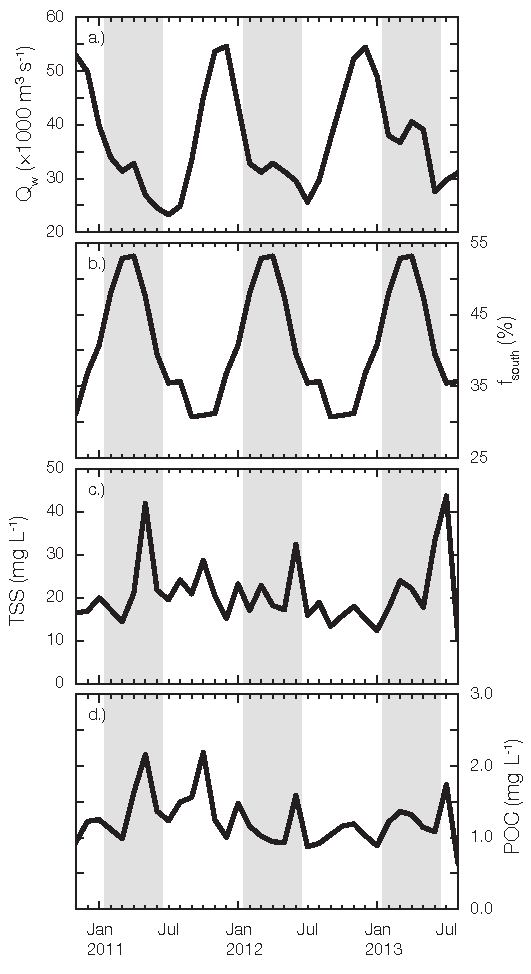
\includegraphics[]{Thesis_Figures/Ch4Fig2}}
	\caption[Environmental parameter time-series plots]{Time series plots of \textit{(A)} Congo River discharge (Q\textsubscript{w}), \textit{(B)} monthly fractional contribution by southern hemisphere tributaries (f\textsubscript{south}) as estimated by \citet{Bricquet:1993ve} (repeating for multiple years), \textit{(C)} TSS concentration, and \textit{(D)} POC concentration measured at Brazzaville/Kinshasa during the sampling period. Southern hemisphere dominated periods are defined when f\textsubscript{south} is greater than the median value of 39\%, and are indicated by gray boxes.}
	\label{Ch4Fig:2} 
\end{figure}

\section{Materials and Methods}

\subsection{Sample collection}

Suspended sediment samples were collected once per month from November 2010 through August 2013 near Brazzaville/Kinshasa, just downstream of Pool Malebo and $\approx 300$ km upstream of the Congo Estuary ($4.3$\textdegree S, $15.3$\textdegree E; Figure \ref{Ch4Fig:1}). The sampling location is downstream of all major tributaries, capturing $>95$\% of the total Congo River catchment, and the effect of the downstream Congo Rapids on bulk organic geochemical properties has been shown to be minimal \citep{Spencer:2012en}. Samples are therefore taken to be representative of material exported to the estuary.

A known volume of surface water ($\approx 25$ L) collected near the center of the channel was filtered through a polyethersulfone (PES) membrane filter (Millipore Corporation) with a nominal pore size of $0.22$ $\mu$m. Filters were dried at $60$\textdegree C for storage and shipment, and sediments were quantitatively re-suspended in $18$M$\Omega$ MilliQ water and freeze-dried in pre-combusted glass jars at $-40$\textdegree C (Christ Alpha-L1 equipped with an in-line cold trap) and weighed for TSS concentration. Discharge was measured concurrently with sample collection via a gauging station operated by the Groupe de Recherche en Sciences Exactes et Naturelles (Republic of Congo) and a rating curve which is periodically updated by Acoustic Doppler Current Profiler (ADCP) transects (Figure \ref{Ch4Fig:2}A). Triplicate transects indicate that precision of discharge measurements is $\pm 5$\%, although overbank flooding during periods of high discharge likely biases measurements towards an underestimate of the true value \citep{Spencer:2014vp}.

\subsection{Extraction, separation, and purification of \textit{n}-alkyl lipids}

After weighing, sediments were homogenized using an agate mortar and pestle and an aliquot was removed for bulk analysis. One sample (June 2013) contained coarse vegetation debris, which was manually removed using solvent-cleaned forceps and weighed separately ($16$ mg; not included in extraction). Sediments were then extracted at $100$\textdegree C for 20 minutes in a microwave accelerated reaction system (MARS, CEM Corporation) in $20$ mL of dichloromethane (DCM) and methanol (9:1). Total lipid extracts were saponified at $70$\textdegree C for 2 hours using $0.5$ M KOH in methanol, after the addition of $\approx$ 1\% $18$M$\Omega$ MilliQ water to prevent methylation of carboxylic acid functional groups. After the addition of $15$ mL of water and $\approx$ 1 g pre-combusted NaCl (to increase density difference), "base" fractions were liquid-liquid extracted in $5$ mL of pure hexane 5 times. Hydrochloric acid was then added until reaching pH $2$, and "acid" fractions were extracted using hexane and DCM (4:1) until the organic phase was clear (generally 5 times). Both acid and base fractions were further purified by column chromatography using $1$ g of Supelclean amino-propyl silica gel (Supelco Analytical) and the following elution scheme: $4$ mL hexane (F1); $7$ mL hexane and DCM (4:1, F2); $10$ mL DCM and acetone (9:1, F3); $14$ mL 2\% (w/w) formic acid in DCM (F4); $18$ mL DCM and methanol (1:1, F5). Acid and base fractions containing alkanes (F1), alcohols (F3), and alkanoic acids (F4) were recombined to ensure maximum recovery.

To isolate \textit{n}-alkanes, F1\textsubscript{T} (acid and base fractions recombined in $1.5$ mL 2:1 hexane:DCM) was subjected to urea adduction in which $500$ $\mu$L of urea-saturated methanol was added and solvent was evaporated using a stream of \ce{N2} gas to promote urea recrystallization (repeated three times). Crystals were rinsed three times with pure hexane to remove the "non adducted" fraction before being dissolved in $15$ mL MilliQ water and liquid-liquid extracted using pure hexane as described above. Both alcohols and alkanoic acids require derivatization in order to be amenable to gas chromatography. Alcohols were acetylated in $250$ $\mu$L of pyridine and acetic anhydride with known isotopic composition (1:1) at $70$\textdegree C for 1 hour. Alkanoic acids were trans-esterified in $15$ mL of HCl and methanol with known isotopic composition (5:95) at $70$\textdegree C for 12 hours. MilliQ water ($15$ mL) was then added, and fatty acid methyl esters (FAMEs) were liquid-liquid extracted into hexane and DCM (4:1) five times. FAMEs were further purified by column chromatography using $1$ g of amino-propyl silica gel eluted with: $4$ mL hexane (F4\textsubscript{T}F1); $7$ mL hexane and DCM (4:1, F4\textsubscript{T}F2); $18$ mL DCM and methanol (1:1, F4\textsubscript{T}F3).

After quantification but before isotope analysis, unsaturated compounds were removed using $0.5$ g silver nitrate silica gel (Supelco Analytical) in a Pasteur pipette column eluted with: $5$ mL hexane and DCM (95:5, SN1); $18$ mL hexane and DCM (4:1, SN2); $5$ mL DCM and acetone (1:1, SN3). Fractions containing \textit{n}-alkanes (F1\textsubscript{T}, adducted), \textit{n}-alcohols (F3\textsubscript{T}, SN2), and \textit{n}-alkanoic acids (F4\textsubscript{T}F2, SN2) were stored at $4$\textdegree C until analyzed. Recovery using this protocol is $\approx 90$\%, as determined by periodically subjecting a known mixture of compounds to the entire procedure.

\subsection{Quantification and isotopic measurements}

Total organic carbon (\%OC) of bulk sediments was measured after decarbonation over HCl fumes at $60$\textdegree C for 72 hours using a Fisons elemental analyzer coupled to a Finnigan Delta\textsuperscript{plus} IRMS as described in \citet{Whiteside:2011jea}. All \textit{n}-alkyl lipids were quantified using a Hewlett Packard 5890 gas chromatograph-flame ionization detector (GC-FID) with a Gerstel PTV injection system, and separated with a VF-1MS capillary column (Agilent Technologies). Temperature program was as follows: ramp to $130$\textdegree C at $30$\textdegree C min\textsuperscript{-1}, ramp to $320$\textdegree C at $8$\textdegree C min\textsuperscript{-1}, hold for 7.5 min at $320$\textdegree C (35min total). Samples were analyzed as a single injection and compared to an external standard run at 3 dilutions between every $\approx$ 5 samples. Uncertainty was calculated using the standard deviation of the best-fit line to the calibration curve.

Compound-specific \ce{\delta^{13}C} was determined using a ThermoFisher Scientific Trace GC Ultra with a DB-1MS capillary column (Agilent Technologies) coupled to a Finnigan MAT252 IRMS via a GC/C combustion interface modified for oxygen trickle flow \citep{Merritt:1995vt,Sessions:2006bn}. Temperature program was as follows: hold for 3 min at $120$\textdegree C, ramp to $200$\textdegree C at $30$\textdegree C min\textsuperscript{-1}, ramp to $320$\textdegree C at $4$\textdegree C min\textsuperscript{-1}, hold for 29.3 min at $320$\textdegree C (70min total). All samples were measured at least in duplicate (triplicate when not limited by low concentrations) and calibrated against pulses of \ce{CO2} gas with a known \ce{\delta^{13}C} value. Long-term precision of an external \textit{n}-alkane standard mixture was $\leq 0.2$\textperthousand\ ($\pm 1\sigma$ standard deviation). Results for individual compounds after correction for derivatization agent are reported with uncertainty as $\pm 1\sigma$ of all injections. Data are reported relative to Vienna Pee-Dee Belemnite (VPDB).

\subsection{Data analysis}

One sample (September 2013) was omitted from the dataset due to contamination by the PES membrane filter, inhibiting the ability to measure bulk \%OC. Additionally, one sample (February 2011) returned spurious \ce{\delta^{13}C} and concentration values, likely due to improper sampling or influence of a local extreme runoff event, and was thus removed in accordance with Chavenet's criterion \citep{Glover:2011tl}. Regressions were performed as weighted least squares (WLS) using a weighting factor of $\sigma^{-1}_{i}$ for each sample $i$ \citep{Glover:2011tl}. All data analysis was performed in the Python programming language v.2.7 and ArcGIS for desktop v.10.3.

\section{Results}

\subsection{Environmental parameters}

All environmental parameters are presented in Table \ref{Ch4Tab:S1}. Congo River discharge recorded at Brazzaville/Kinshasa during the sampling period ranged from a minimum of $23.2 \times 10^3 \pm 1.1 \times 10^3$ m\textsuperscript{3} sec\textsuperscript{-1} in July 2011 to a maximum of $54.6 \times 10^3 \pm 2.7 \times 10^3$ m\textsuperscript{3} sec\textsuperscript{-1} in December 2011 (Figure \ref{Ch4Fig:2}A). Average discharge for 2011 ($35.3 \times 10^3$ m\textsuperscript{3} sec\textsuperscript{-1}) was the fifth-lowest since recording began in 1977, while 2012 and 2013 were closer to long-term average values \citep{Spencer:2012en}. Seasonally, discharge displays two maxima: a large peak in Nov-Dec-Jan during high flow through northern hemisphere tributaries and the main-stem \textit{Cuvette Congolaise}, and a smaller peak in Mar-Apr-May due to increased flow from southern hemisphere tributaries \citep{Bricquet:1993ve,Coynel:2005cn,Bouillon:2012cw,Spencer:2012en,Spencer:2014vp}. This leads to an estimated range in southern-hemisphere contribution (termed f\textsubscript{south}) of 31--53\%, with a median value of 39\% \citep{Bricquet:1993ve}. We classify periods with f\textsubscript{south} above the median value -- \textit{\textit{i.e.}} February through May -- as being "southern hemisphere dominated," and all other times as being "main-stem dominated" or "\textit{Cuvette Congolaise} dominated" (Figure \ref{Ch4Fig:2}B). Importantly, the largest southern-hemisphere tributary, the Kasai River, enters the main-stem downstream of the \textit{Cuvette Congolaise} swamp forest.

TSS concentration averaged $21.1 \pm 7.6$ g m\textsuperscript{-3} throughout the time series, ranging from a minimum of $10.2$ g m\textsuperscript{-3} to a maximum of $43.6$ g m\textsuperscript{-3} (Figure \ref{Ch4Fig:2}C). TSS are rich in carbon, with an average \%OC of $6.1 \pm 1.0$\%, leading to an average particulate organic carbon (POC) concentration of $1.3 \pm 0.4$ g m\textsuperscript{-3} with a range of $0.6 - 2.6$ g m\textsuperscript{-3} (Figure \ref{Ch4Fig:2}D). TSS, POC, and \%OC ranges reported here agree well with published values, both for the main-stem Congo as well as the Oubangui River at Bangui Station (Figure \ref{Ch4Fig:1}), a major right-bank tributary \citep{Coynel:2005cn,Bouillon:2012cw,Bouillon:2014ko}. Congo River suspended sediment \%OC increases slightly as a function of discharge ($R^2 = 0.19$, $p$-value = $0.01$; not shown), although POC concentration shows no correlation with discharge ($p$-value > $0.05$; not shown). 

% Figure 3
\begin{figure}[t]
	\makebox[\textwidth][c]{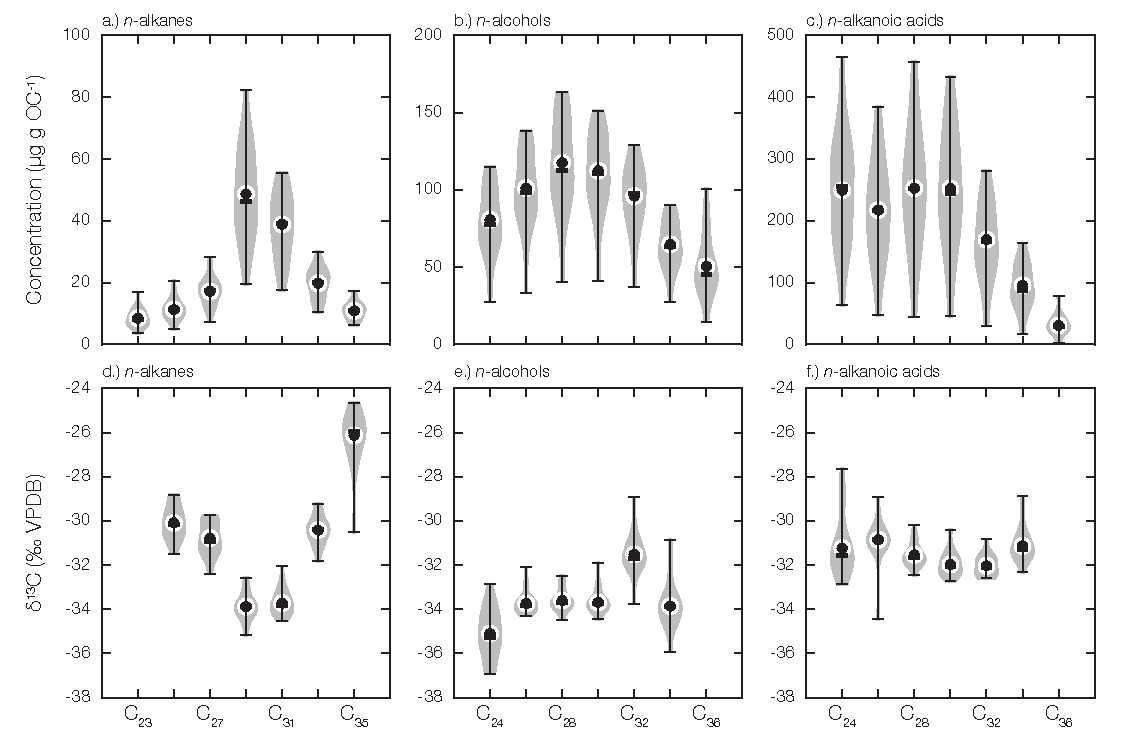
\includegraphics[]{Thesis_Figures/Ch4Fig3}}
	\caption[Concentration and \ce{\delta^{13}C} violin plots]{Violin plots of \textit{n}-alkane, \textit{n}-alcohol, and \textit{n}-alkanoic acid \textit{(A)--(C)} POC-normalized concentrations and \textit{(D)--(F)} \ce{\delta^{13}C} values for individual long-chain homologues. Violin plots represent the temporal distribution of values throughout the time-series using a Gaussian kernel density function. Mean values are marked as black circles, and median values are marked as horizontal black lines.}
	\label{Ch4Fig:3} 
\end{figure}

\subsection{Lipid abundance and distribution}

Concentrations of individual homologues, average chain lengths, and carbon preference indices are presented in Tables \ref{Ch4Tab:S2}--\ref{Ch4Tab:S4}.

\subsubsection{\textit{n}-Alkanes}

Carbon-normalized concentrations of individual plant-wax \textit{n}-alkanes (C\textsubscript{23}--C\textsubscript{35}; odd-numbered homologues) range from a minimum of $3.7 \pm 0.8$ $\mu$g gOC\textsuperscript{-1} (C\textsubscript{23}) to a maximum of $82.1 \pm 1.3$ $\mu$g gOC\textsuperscript{-1} (C\textsubscript{29}; Figure \ref{Ch4Fig:3}A). The sum of the long-chain odd-numbered homologue concentrations ($\Sigma$LC\textsubscript{25-35}) exhibits considerably less variability, ranging from $66.0 - 207.1$ $\mu$g gOC\textsuperscript{-1}. Time-series plots of $\Sigma$LC\textsubscript{25-35} and selected homologue concentrations are presented in Figure \ref{Ch4Fig:4}A--C. $\Sigma$LC\textsubscript{25-35} concentrations show a slight decrease with increasing discharge (Figure \ref{Ch4Fig:5}A), although this relationship is driven by changes in \%OC and disappears when considering sediment-normalized concentrations ($R^2 = 0.001$, $p$-value > $0.05$; not shown).

\textit{n}-Alkanes are consistently dominated by C\textsubscript{29} and C\textsubscript{31} homologues, contributing up to 33\% and 26\% to $\Sigma$LC\textsubscript{25-35}, respectively. At only 8--9\% each, C\textsubscript{25} and C\textsubscript{35} are the least abundant homologues, while C\textsubscript{27} and C\textsubscript{33} contribute 12--13\% each. To compare changes in distributions between samples, we compute the average chain length (ACL) as the concentration-weighted average of C\textsubscript{25}--C\textsubscript{35} odd-numbered homologues:

% Equation 1
\begin{equation}\label{Ch4Eq:1}
\text{ACL} = \frac{25\times[\ce{C}_{25}] + 27\times[\ce{C}_{27}] + 29\times[\ce{C}_{29}] + 31\times[\ce{C}_{31}] + 33\times[\ce{C}_{33}] + 35\times[\ce{C}_{35}]}{\Sigma \text{LC}_{25-35}}
\end{equation}

\textit{n}-Alkane ACL in our sample set is remarkably stable, with an average of $30.0 \pm 0.1$ units and a range of $29.6 - 30.2$ units, and shows no significant correlation with discharge (Figure \ref{Ch4Fig:5}B). We compute the carbon preference index (CPI) for C\textsubscript{25}--C\textsubscript{35}, defined as: 

% Equation 2
\begin{equation}\label{Ch4Eq:2}
\text{CPI} = \frac{1}{2} \left( \frac{\Sigma \text{LC}_{25-35}}{\Sigma \text{LC}_{24-34}} + \frac{\Sigma \text{LC}_{25-35}}{\Sigma \text{LC}_{26-36}} \right)
\end{equation}

$\Sigma$LC\textsubscript{25-35} refers to odd-numbered homologues only while $\Sigma$LC\textsubscript{24-34} and $\Sigma$LC\textsubscript{26-36} refer to even-numbered homologues only (we note that C\textsubscript{36} was not detected in any sample). \textit{n}-Alkane CPI in our dataset averages $2.9 \pm 0.5$, ranging from $2.1 - 4.1$, and shows a small yet statistically significant decrease with increasing discharge (Figure \ref{Ch4Fig:5}C).

We additionally calculate P\textsubscript{aq}, an estimate of macrophyte contribution to \textit{n}-alkanes \citep{Ficken:2000wq} as:

% Equation 3
\begin{equation}\label{Ch4Eq:3}
\text{P}_{\text{aq}} = \frac{[\ce{C}_{23}] + [\ce{C}_{25}]}{[\ce{C}_{23}] + [\ce{C}_{25}] + [\ce{C}_{27}] + [\ce{C}_{29}]}
\end{equation}

Resulting P\textsubscript{aq} values in our sample set (Table \ref{Ch4Tab:S2}) average $0.19 \pm 0.04$ with a range of $0.12 - 0.26$, and are uncorrelated with discharge ($R^2 = 0.08$, $p$-value > $0.05$; not shown).

% Figure 4
\begin{figure}[p]
	\makebox[\textwidth][c]{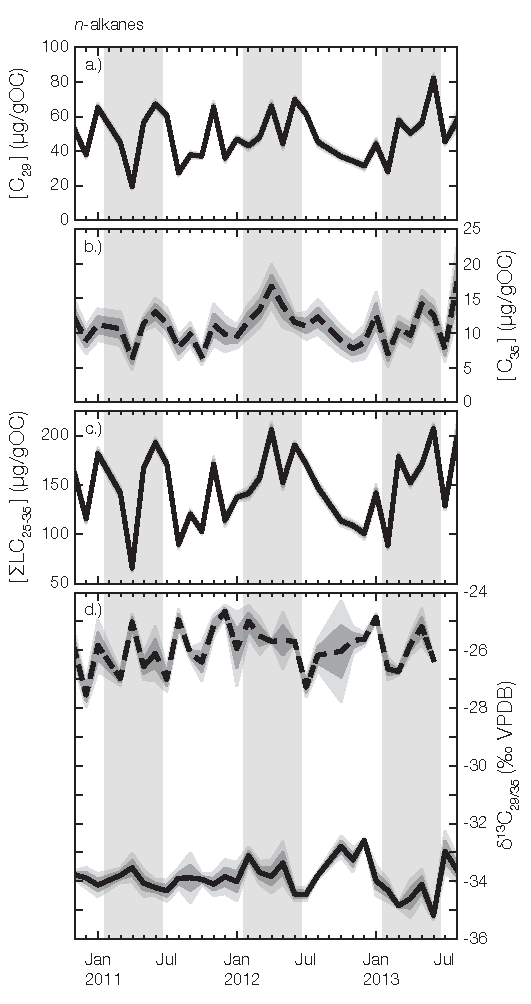
\includegraphics[]{Thesis_Figures/Ch4Fig4}}
	\caption[\textit{n}-alkane concentration and \ce{\delta^{13}C} time-series plots]{Time series plots of \textit{n}-alkane concentrations -- \textit{(A)} C\textsubscript{29}, \textit{(B)} C\textsubscript{35}, \textit{(C)} $\Sigma$LC\textsubscript{25-35} -- and \ce{\delta^{13}C} values -- \textit{(D)} C\textsubscript{29} (solid line) and C\textsubscript{35} (dashed line). Selected homologues are chosen to represent the increasing influence by C\textsubscript{4} grasses with increasing chain length. Dark gray shading represents $\pm 1\sigma$ uncertainty, and light gray shading represents 95\% confidence interval (CI). Periods when f\textsubscript{south} > 39\% are indicated by gray boxes.}
	\label{Ch4Fig:4} 
\end{figure}

% Figure 5
\begin{figure}[p]
	\makebox[\textwidth][c]{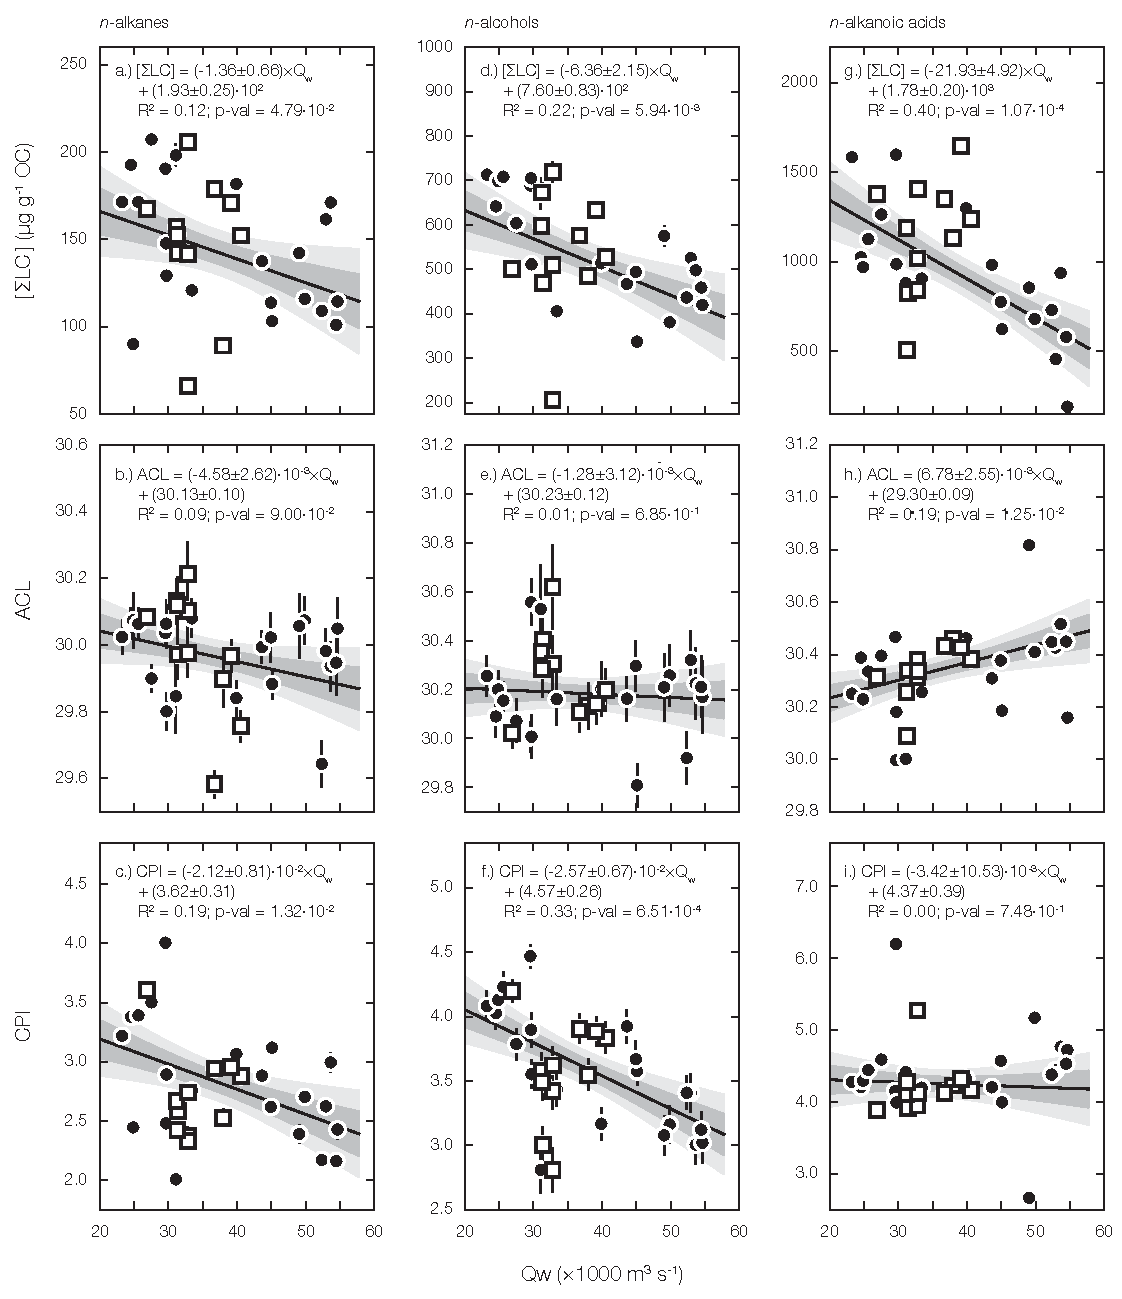
\includegraphics[scale=0.9]{Thesis_Figures/Ch4Fig5}}
	\caption[Correlations between concentration, ACL, CPI, and discharge]{Correlations between $\Sigma$LC\textsubscript{25-35}/$\Sigma$LC\textsubscript{26-36} concentrations, ACL, and CPI vs. Congo River discharge (Q\textsubscript{w}) measured at Brazzaville/Kinshasa for \textit{n}-alkanes \textit{(A)--(C)}, \textit{n}-alcohols \textit{(D)--(F)}, and \textit{n}-alkanoic acids \textit{(G)--(I)}. Error bars on individual points represent $\pm 1 \sigma$ uncertainty. Black line is the WLS best-fit line, dark gray shading represents $\pm 1 \sigma$  regression uncertainty, and light gray shading represents the 95\% CI. Samples collected when f\textsubscript{south} > 39\% are plotted as white squares, and samples collected when f\textsubscript{south} $\leq$ 39\% are plotted as black circles.}
	\label{Ch4Fig:5} 
\end{figure}

\subsubsection{\textit{n}-Alcohols}

While nominally regarded as a plant-wax lipid, C\textsubscript{24} \textit{n}-alcohol has been observed in freshwater phytoplankton \citep{Volkman:1998tk,Volkman:1999tq,Xu:2007jk}. In our sample set, isotopic evidence indicates that phytoplankton contribute to C\textsubscript{24} \textit{n}-alcohol (see section \ref{Ch4Sec:52} below), and we therefore omit this compound from our calculations of ACL, CPI, and $\Sigma$LC. 

Plant-wax \textit{n}-alcohols (C\textsubscript{26}--C\textsubscript{36}; even-numbered homologues) are considerably more abundant than \textit{n}-alkanes, with individual compound concentrations ranging from $14.6 \pm 3.1$ $\mu$g gOC\textsuperscript{-1} (C\textsubscript{36}) to $163.0 \pm 8.0$ $\mu$g gOC\textsuperscript{-1} (C\textsubscript{28}; Figure \ref{Ch4Fig:3}B). $\Sigma$LC\textsubscript{26-36} concentrations range from $206.5 - 718.7$ $\mu$g gOC\textsuperscript{-1}, and are therefore $3.8 \pm 0.9$ times higher than corresponding \textit{n}-alkane concentrations. Time series plots of $\Sigma$LC\textsubscript{26-36} and selected homologue concentrations are shown in Figure \ref{Ch4Fig:6}A--C, while Figure \ref{Ch4Fig:5}D shows that $\Sigma$LC\textsubscript{26-36} concentrations decrease as a function of river discharge. Again, this relationship is driven by changes in \%OC, as sediment-normalized $\Sigma$LC\textsubscript{26-36} concentrations display no significant relationship with discharge ($R^2 = 0.04$, $p$-value > $0.05$; not shown).

\textit{n}-Alcohols are more evenly distributed than \textit{n}-alkanes, with no single homologue contributing more than 21\% or less than 9\% of the long-chain total (Figure \ref{Ch4Fig:3}B). ACL is calculated similarly to \textit{n}-alkanes, but using C\textsubscript{26}--C\textsubscript{36} even-numbered homologues. Again, ACL shows little variability, with a range of $29.8 - 30.6$ units and an average of $30.2 \pm 0.2$ units. CPI, calculated as above but using $\Sigma$LC\textsubscript{26-36} in the numerator and $\Sigma$LC\textsubscript{25-35}/$\Sigma$LC\textsubscript{27-37} in the denominators (noting that C\textsubscript{37} was not detected in any sample), averages $3.7 \pm 0.4$ with a range of $3.0 - 4.6$. While ACL shows no correlation (Figure \ref{Ch4Fig:5}E), CPI exhibits a strong negative relationship with discharge (Figure \ref{Ch4Fig:5}F).

% Figure 6
\begin{figure}[p]
	\makebox[\textwidth][c]{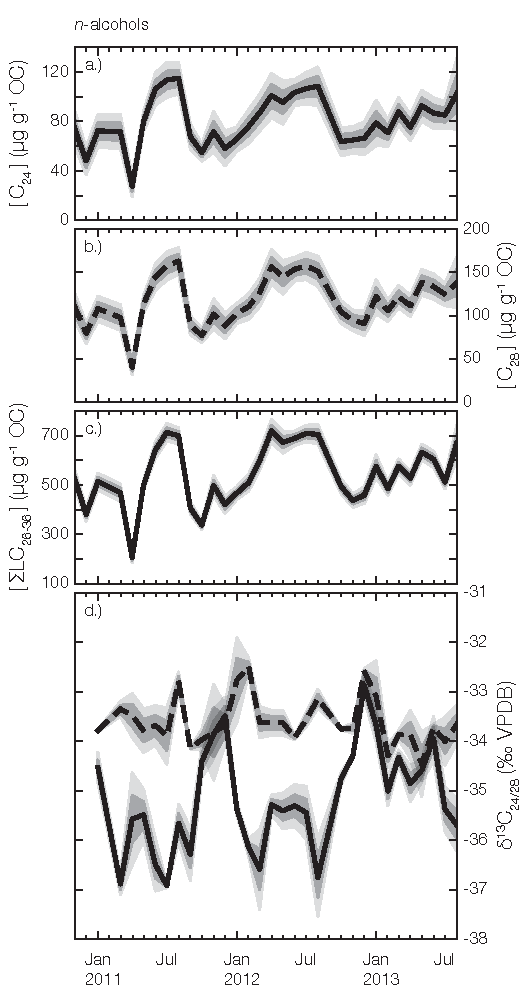
\includegraphics[]{Thesis_Figures/Ch4Fig6}}
	\caption[\textit{n}-alcohol concentration and \ce{\delta^{13}C} time-series plots]{Time series plots of \textit{n}-alcohol concentrations -- \textit{(A)} C\textsubscript{24}, \textit{(B)} C\textsubscript{28}, \textit{(C)} $\Sigma$LC\textsubscript{26-36} -- and \ce{\delta^{13}C} values -- \textit{(D)} C\textsubscript{24} (solid line) and C\textsubscript{28} (dashed line). Selected homologues are chosen to represent the autochthonous contribution to C\textsubscript{24} and C\textsubscript{3} plant dominance of longer homologues. Dark gray shading represents $\pm 1\sigma$ uncertainty, and light gray shading represents 95\% confidence interval (CI). Periods when f\textsubscript{south} > 39\% are indicated by gray boxes.}
	\label{Ch4Fig:6} 
\end{figure}

\subsubsection{\textit{n}-Alkanoic acids}

As C\textsubscript{24} \textit{n}-alcohol was omitted from the above calculations, to accurately compare ACL, CPI, and $\Sigma$LC across compound classes we remove C\textsubscript{24} \textit{n}-alkanoic acid from the calculations performed here.

Plant-wax \textit{n}-alkanoic acid concentrations (C\textsubscript{26}--C\textsubscript{36}; even-numbered homologues) display the highest values and largest variability of all \textit{n}-alkyl lipid classes (Figure \ref{Ch4Fig:3}C). Individual compounds range from $2.7 \pm 0.2$ $\mu$g gOC\textsuperscript{-1} (C\textsubscript{36}) to $457.1 \pm 2.3$ $\mu$g gOC\textsuperscript{-1} (C\textsubscript{28}), with a $\Sigma$LC\textsubscript{26-36} concentration range of $190.2 - 1648.6$ $\mu$g gOC\textsuperscript{-1}. Long-chain \textit{n}-alkanoic acids therefore contribute up to $\approx 0.2$\% of total exported POC, and are $7.1 \pm 2.5$ times more abundant than \textit{n}-alkanes. Similar to \textit{n}-alkanes and \textit{n}-alcohols, \textit{n}-alkanoic acid carbon-normalized $\Sigma$LC\textsubscript{26-36} concentrations decrease with increasing river discharge (Figure \ref{Ch4Fig:5}G). While this relationship is partially driven by changes in \%OC, sediment-normalized values additionally exhibit a statistically significant decrease ($R^2 = 0.19$, $p$-value = $1.4 \times 10^{-2}$; not shown). Time series plots of selected homologues and $\Sigma$LC\textsubscript{26-36} concentrations are plotted in Figure \ref{Ch4Fig:7}A--C.

\textit{n}-Alkanoic acids display a similar distribution to \textit{n}-alcohols, with C\textsubscript{26}, C\textsubscript{28}, and C\textsubscript{30} all contributing $\approx 20 - 25$\% of the long-chain total, and decreasing contribution with increasing chain length beyond C\textsubscript{30} (Figure \ref{Ch4Fig:3}C). Average ACL is $29.5 \pm 0.2$, slightly lower than that of \textit{n}-alkanes and \textit{n}-alcohols, and exhibits a slight increase with increasing discharge (Figure \ref{Ch4Fig:5}H). \textit{n}-Alkanoic acid CPI is the highest of all observed compound classes (C\textsubscript{37} not detected), averaging $4.3 \pm 0.5$ and shows no correlation with river discharge (Figure \ref{Ch4Fig:5}I). We note that inclusion of \textit{n}-C\textsubscript{24} decreases ACL to $28.4 \pm 0.2$ and exhibits no effect on CPI (not shown).

% Figure 7
\begin{figure}[p]
	\makebox[\textwidth][c]{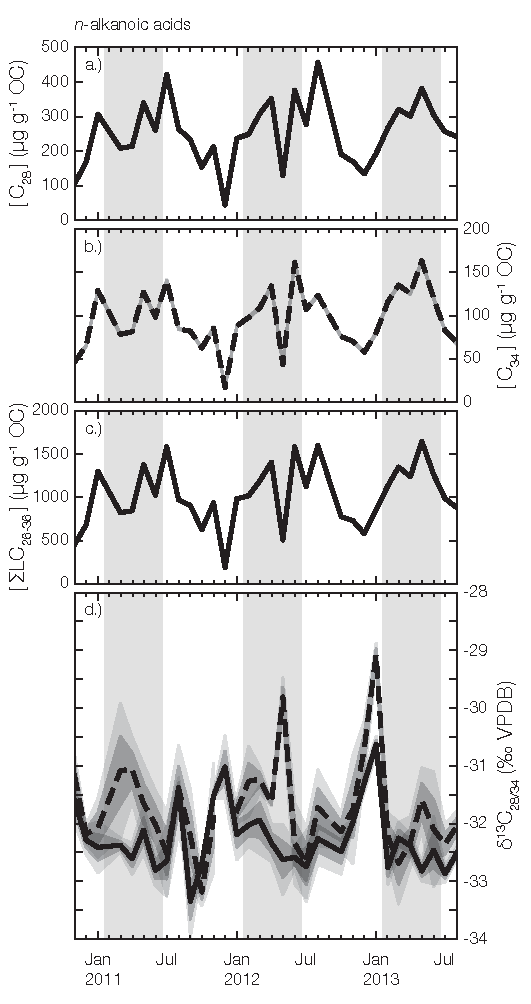
\includegraphics[]{Thesis_Figures/Ch4Fig7}}
	\caption[\textit{n}-alkanoic acid concentration and \ce{\delta^{13}C} time-series plots]{Time series plots of \textit{n}-alkanoic acid concentrations -- \textit{(A)} C\textsubscript{28}, \textit{(B)} C\textsubscript{34}, \textit{(C)} $\Sigma$LC\textsubscript{26-36} -- and \ce{\delta^{13}C} values -- \textit{(D)} C\textsubscript{28} (solid line) and C\textsubscript{34} (dashed line). Selected homologues are chosen to represent the similar C\textsubscript{3}-like isotopic composition across all long-chain homologues. Dark gray shading represents $\pm 1\sigma$ uncertainty, and light gray shading represents 95\% confidence interval (CI). Periods when f\textsubscript{south} > 39\% are indicated by gray boxes.}
	\label{Ch4Fig:7}
\end{figure}

\subsection{Compound-specific \ce{\delta^{13}C}}

Individual homologue \ce{\delta^{13}C} measurements are reported in Tables \ref{Ch4Tab:S5}--\ref{Ch4Tab:S7}.

\subsubsection{\textit{n}-Alkanes}

\textit{n}-Alkanes display the largest \ce{\delta^{13}C} variability across long-chain homologues of all compound classes studied, with an average spread (max -- min) of $8.1 \pm 0.7$\textperthousand\ (Figure \ref{Ch4Fig:3}D). However, we note that C\textsubscript{25} could not be measured in two samples (December 2010, July 2013) and C\textsubscript{35} could not be measured in one sample (July 2013), as concentrations were too low. All samples show the same general trend with chain length -- \textit{i.e.} C\textsubscript{25}, C\textsubscript{27}, and C\textsubscript{33} near $-30$\textperthousand, C\textsubscript{29} and C\textsubscript{31} near $-34$\textperthousand, and C\textsubscript{35} up to $-24.7 \pm 0.1$\textperthousand\ (Figure \ref{Ch4Fig:3}D). Temporal variability for each compound in the dataset is $\approx 2.5 - 3.0$\textperthousand\ (max -- min), as is shown for C\textsubscript{29} and C\textsubscript{35} in Figure \ref{Ch4Fig:4}D. \ce{\delta^{13}C} values of all compounds are uncorrelated with discharge ($p$-value > $0.05$; not shown).

\subsubsection{\textit{n}-Alcohols}

Low concentrations prevented the measurement of \ce{\delta^{13}C} values for C\textsubscript{36} \textit{n}-alcohol. Additionally, one sample (December 2010) displayed contamination by siloxanes and was omitted. All remaining samples follow the same general pattern, with C\textsubscript{24} exhibiting the most depleted values, nearly identical values for C\textsubscript{26}--C\textsubscript{30} and C\textsubscript{34}, and C\textsubscript{32} showing the most enrichment, averaging $-31.1 \pm 0.7$\textperthousand\ (Figure \ref{Ch4Fig:3}E).

Time series plots of \ce{\delta^{13}C} values for C\textsubscript{24} and C\textsubscript{28} \textit{n}-alcohols are plotted in Figure \ref{Ch4Fig:6}D. C\textsubscript{24} \ce{\delta^{13}C} values display a strong positive correlation with discharge (Figure \ref{Ch4Fig:8}A), with the most \ce{^{13}C}-depleted value ($-36.9 \pm 0.1$\textperthousand) observed during the lowest measured discharge on record (July 2011). In contrast, C\textsubscript{28}--C\textsubscript{34} \ce{\delta^{13}C} values display no correlation with discharge ($p$-value > $0.05$; not shown), although C\textsubscript{26} exhibits a slight positive relationship, mainly driven by three outlier points (Figure \ref{Ch4Fig:8}B). Resulting \ce{\delta^{13}C} spread across measured plant-wax \textit{n}-alcohols (\textit{\textit{i.e.}} C\textsubscript{26}--C\textsubscript{34}) is therefore $2.6 \pm 0.6$\textperthousand, significantly lower than that for \textit{n}-alkanes, even when only considering analogous homologues (\textit{i.e.} C\textsubscript{25}--C\textsubscript{33} \textit{n}-alkane spread of $4.2 \pm 0.6$\textperthousand). While temporal variability within C\textsubscript{26}--C\textsubscript{30} homologues is $\approx 2.5$\textperthousand, C\textsubscript{32} and C\textsubscript{34} are significantly more variable, with a max -- min value of $\approx 3.5$\textperthousand. 

% Figure 8
\begin{figure}[p]
	\makebox[\textwidth][c]{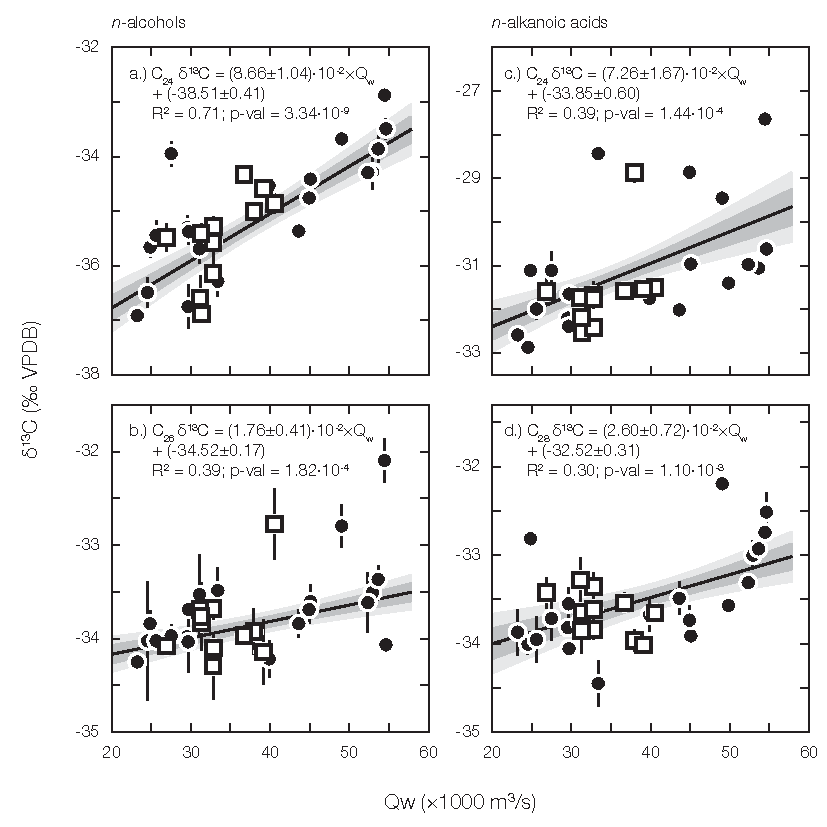
\includegraphics[]{Thesis_Figures/Ch4Fig8}}
	\caption[Correlations between \ce{\delta^{13}C} and discharge]{Correlations between \ce{\delta^{13}C} values vs. Congo River discharge (Q\textsubscript{w}) measured at Brazzaville/Kinshasa for \textit{(A)} C\textsubscript{24} \textit{n}-alcohol, \textit{(B)} C\textsubscript{26} \textit{n}-alcohol, \textit{(C)} C\textsubscript{24} \textit{n}-alkanoic acid, and \textit{(D)} C\textsubscript{28} \textit{n}-alkanoic acid. Error bars on individual points represent $\pm 1 \sigma$ uncertainty. Black line is the WLS best-fit line, dark gray shading represents $\pm 1 \sigma$ regression uncertainty, and light gray shading represents the 95\% CI. Samples collected when f\textsubscript{south} > 39\% are plotted as white squares, and samples collected when f\textsubscript{south} $\leq$ 39\% are plotted as black circles.}
	\label{Ch4Fig:8} 
\end{figure}

\subsubsection{\textit{n}-Alkanoic acids}

C\textsubscript{36} \textit{n}-alkanoic acid \ce{\delta^{13}C} values could not be measured as concentrations were too low, nor could C\textsubscript{34} in one sample (December 2011). Similar to \textit{n}-alcohols, \textit{n}-alkanoic acids show significantly less spread in \ce{\delta^{13}C} values between measured homologues (\textit{i.e.} C\textsubscript{24}--C\textsubscript{34}; $2.0 \pm 1.1$\textperthousand) than do \textit{n}-alkanes (Figure \ref{Ch4Fig:3}F). C\textsubscript{24} and C\textsubscript{26} \textit{n}-alkanoic acids display the largest temporal variability of all measured compounds with a range of $5.2$\textperthousand\ and $5.5$\textperthousand, respectively. In contrast, C\textsubscript{28}--C\textsubscript{32} temporal variability is $\approx 2.5$\textperthousand, similar to that for \textit{n}-alkanes and \textit{n}-alcohols, while C\textsubscript{34} varies by $3.4$\textperthousand\ (Figure \ref{Ch4Fig:7}D).

Unlike \textit{n}-alcohols, C\textsubscript{24} \textit{n}-alkanoic acids do not show \ce{^{13}C}-depletion relative to longer chain homologues during periods of low discharge ($p$-value > $0.05$; not shown). In addition, C\textsubscript{24}--C\textsubscript{26} \textit{n}-alkanoic acids are \ce{^{13}C}-eriched relative to C\textsubscript{24} \textit{n}-alcohol by $3.9 \pm 1.1$\textperthousand\ and $4.3 \pm 1.3$\textperthousand, respectively. C\textsubscript{24} and C\textsubscript{28} \ce{\delta^{13}C} values show a small yet statistically significant enrichment with increasing discharge (Figure \ref{Ch4Fig:8}C--D), while all other compounds are uncorrelated ($p$-value > $0.05$; not shown).

\subsection{Correlations between homologues and compound classes}

WLS regression correlation coefficients ($r$) and significance $p$-values for concentrations and \ce{\delta^{13}C} values of each compound are presented in Tables \ref{Ch4Tab:1}--\ref{Ch4Tab:3}. 

Within each \textit{n}-alkyl compound class, concentrations of all long-chain homologues exhibit statistically significant positive correlations, with $r$ ranging from $0.52 - 0.94$ for \textit{n}-alkanes, $0.71 - 0.98$ for \textit{n}-alcohols, and $0.70 - 0.99$ for \textit{n}-alkanoic acids. In contrast, concentrations of long-chain homologues between different compound classes are uncorrelated or display weak positive correlation ($r \leq 0.75$). Concentrations of both C\textsubscript{23} and C\textsubscript{25} \textit{n}-alkane are statistically uncorrelated with their corresponding (\textit{i.e.} $n + 1$) \textit{n}-alkanoic acids. Additionally, C\textsubscript{23}, C\textsubscript{25}, and C\textsubscript{35} \textit{n}-alkane concentrations are uncorrelated with those of C\textsubscript{28}--C\textsubscript{34} \textit{n}-alkanoic acid; C\textsubscript{36} \textit{n}-alcohol is uncorrelated with C\textsubscript{30}--C\textsubscript{36} \textit{n}-alkanoic acid; and C\textsubscript{29} \textit{n}-alkane is uncorrelated with C\textsubscript{36} \textit{n}-alcohol, indicating a decoupling between the sources of these compounds.

In general, \ce{\delta^{13}C} values between all long-chain homologues exhibit less correlation than do concentrations. Within each compound class, $r$ exhibits a range of $-0.02$ to $0.75$ for \textit{n}-alkanes, $-0.09$ to $0.50$ for \textit{n}-alcohols, and $-0.55$ to $0.79$ for \textit{n}-alkanoic acids. Similar ranges are observed between compound classes: $-0.09$ to $0.78$ between \textit{n}-alkanes and \textit{n}-alcohols, $-0.16$ to $0.63$ between \textit{n}-alkanes and \textit{n}-alkanoic acids, and $-0.35$ to $0.58$ between \textit{n}-alcohols and \textit{n}-alkanoic acids. Interestingly, \ce{\delta^{13}C} values between C\textsubscript{26} and C\textsubscript{34} \textit{n}-alkanoic acids display a statistically significant negative correlation, while all other significant correlations are positive.

Lastly, \ce{\delta^{13}C} values are generally either uncorrelated with concentrations or display a statistically significant negative correlation. C\textsubscript{27}--C\textsubscript{33} \textit{n}-alkane, C\textsubscript{24} \textit{n}-alcohol, and C\textsubscript{24} \textit{n}-alkanoic acid \ce{\delta^{13}C} values all exhibit significant negative correlation with increasing concentrations of most measured compounds, while C\textsubscript{25} \textit{n}-alkane, C\textsubscript{35} \textit{n}-alkane, C\textsubscript{28}--C\textsubscript{30} \textit{n}-alcohol, and C\textsubscript{34} \textit{n}-alcohol \ce{\delta^{13}C} values are statistically uncorrelated with the concentrations of all compounds. In contrast to other compound classes, some \textit{n}-alkanoic acid \ce{\delta^{13}C} values exhibit significant positive correlation with concentrations: C\textsubscript{30} \ce{\delta^{13}C} values correlate positively with C\textsubscript{33}--C\textsubscript{35} \textit{n}-alkane and C\textsubscript{36} \textit{n}-alcohol concentrations, C\textsubscript{32} \ce{\delta^{13}C} values correlate positively with C\textsubscript{36} \textit{n}-alcohol concentrations, and C\textsubscript{34} \ce{\delta^{13}C} values correlate positively with C\textsubscript{36} \textit{n}-alkanoic acid concentrations. 

% Table 1
\begin{sidewaystable}[p]
	\caption[C\textsubscript{23+} concentration correlation $r$ and $p$-values]{Weighted least squares regression correlation values ($r$) and significance $p$-values between all measured C\textsubscript{23+} \textit{n}-alkyl lipid concentrations. Statistically significant ($p$-value $\leq  0.05$) correlations are bolded.}
	\centering
		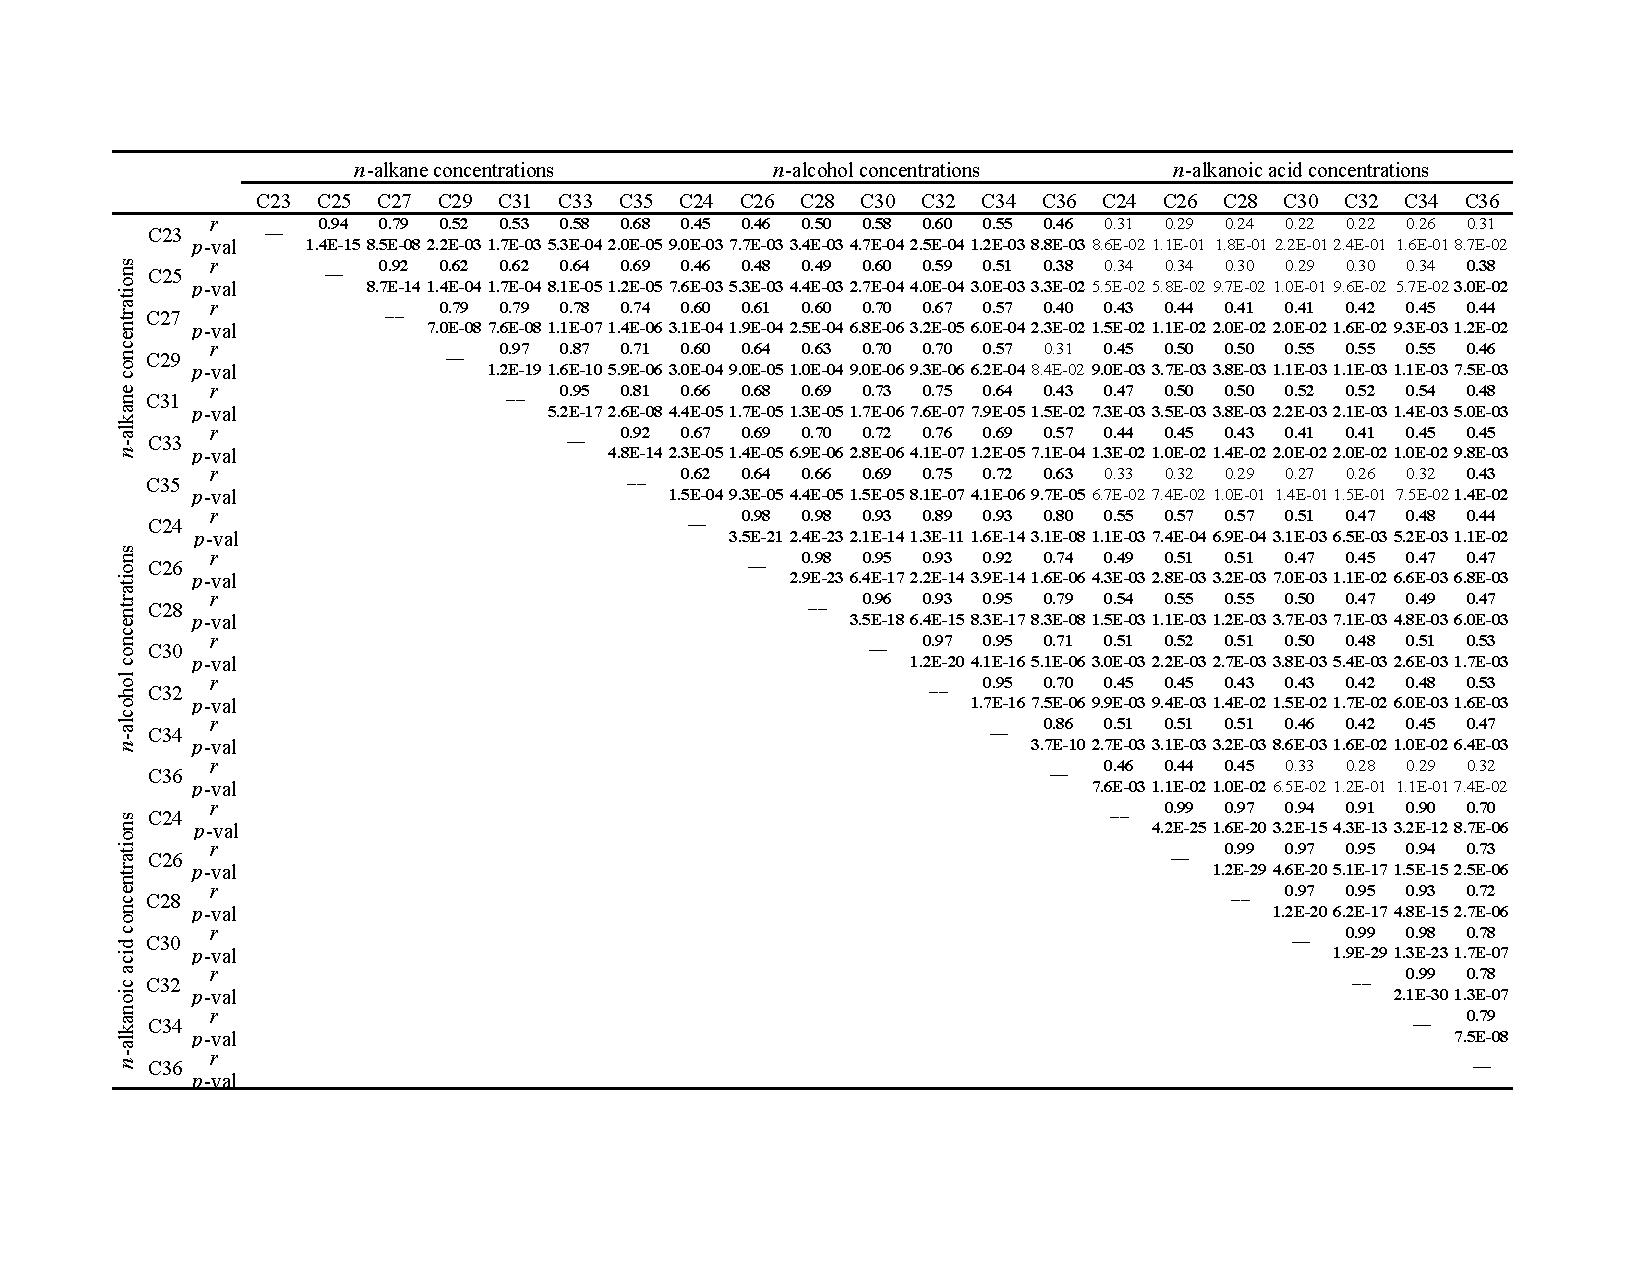
\includegraphics{Thesis_Tables/Ch4Tab1}
	\label{Ch4Tab:1} 
\end{sidewaystable}

% Table 2
\begin{sidewaystable}[p]
	\caption[C\textsubscript{25+} \ce{\delta^{13}C} correlation $r$ and $p$-values]{Weighted least squares regression correlation values ($r$) and significance $p$-values between all measured C\textsubscript{25+} \textit{n}-alkyl lipid \ce{\delta^{13}C} values. Statistically significant ($p$-value $\leq  0.05$) correlations are bolded.}
	\centering
		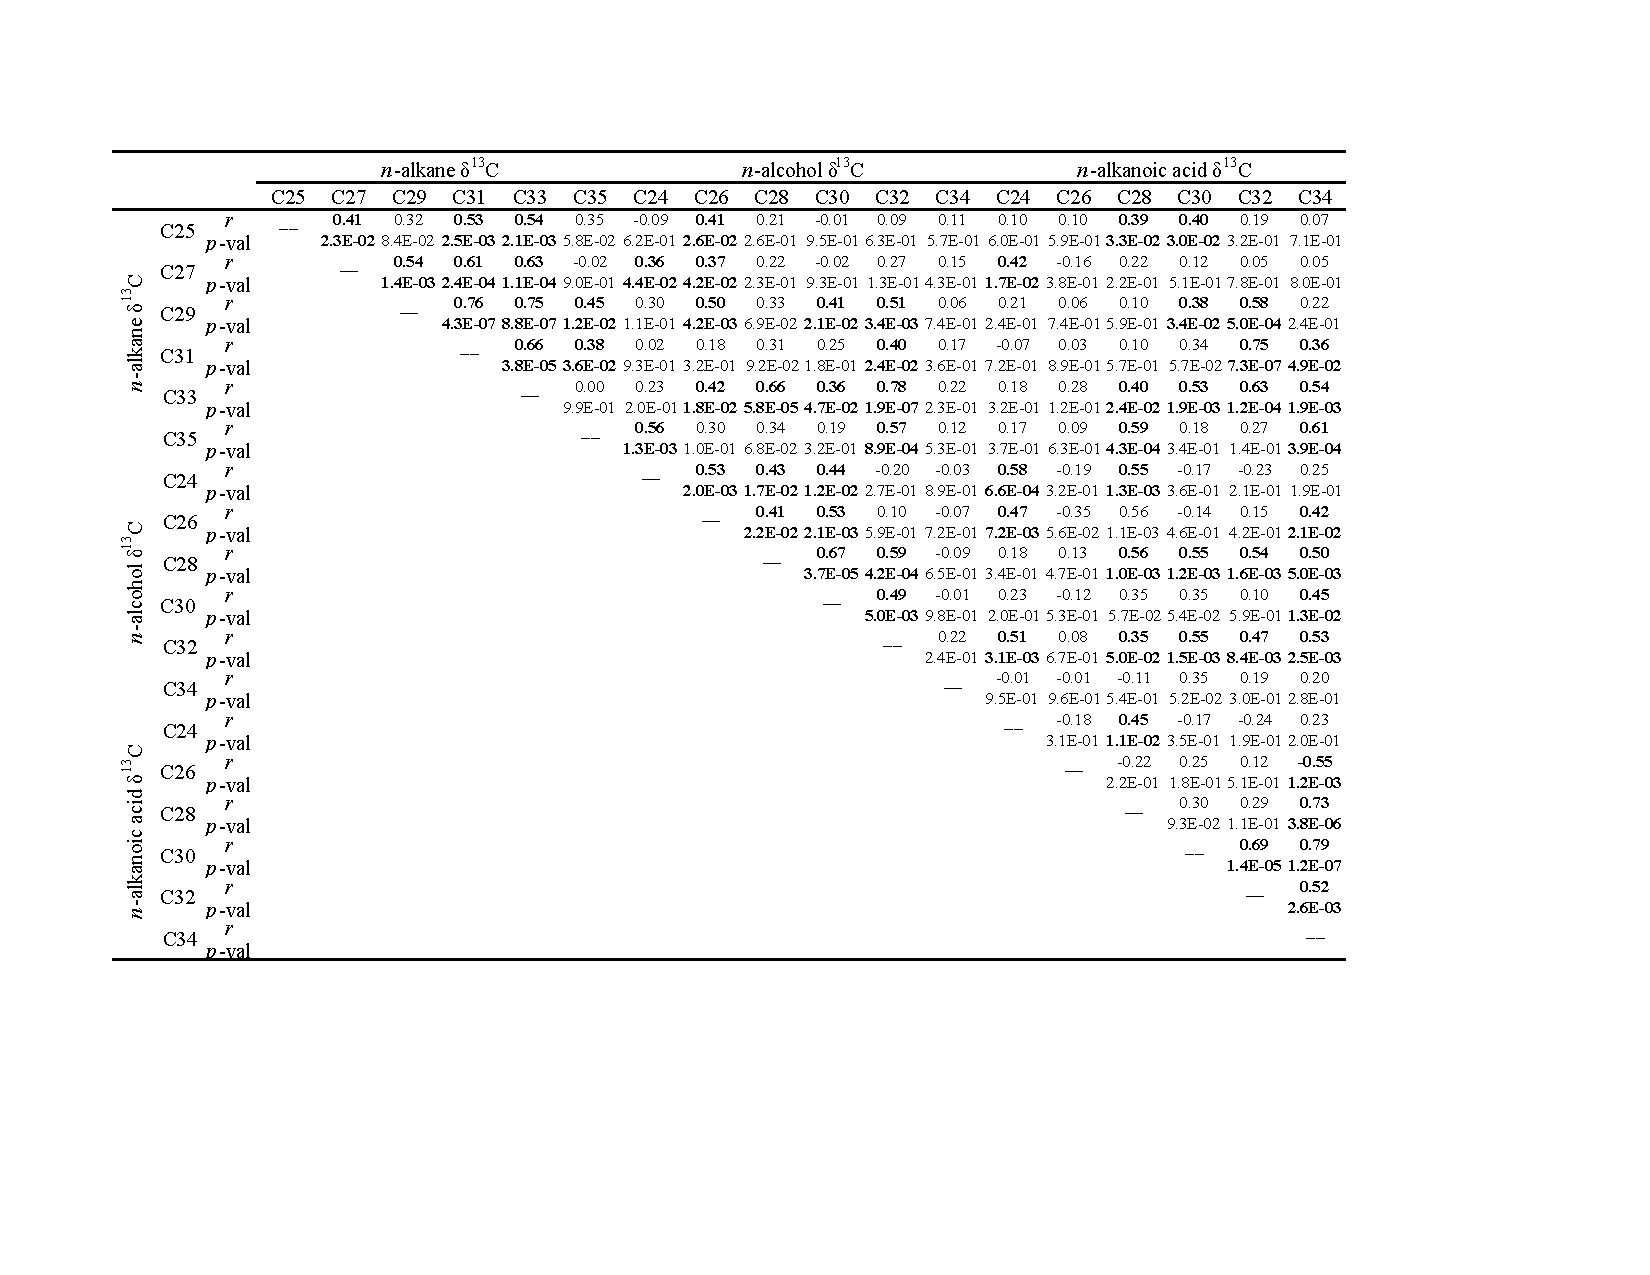
\includegraphics{Thesis_Tables/Ch4Tab2}
	\label{Ch4Tab:2} 
\end{sidewaystable}

% Table 3
\begin{sidewaystable}[p]
	\caption[C\textsubscript{25+} concentration vs. \ce{\delta^{13}C} correlation $r$ and $p$-values]{Weighted least squares regression correlation values ($r$) and significance $p$-values between all measured C\textsubscript{23+} \textit{n}-alkyl lipid concentrations vs. C\textsubscript{25+} \ce{\delta^{13}C} values. Statistically significant ($p$-value $\leq  0.05$) correlations are bolded.}
	\centering
		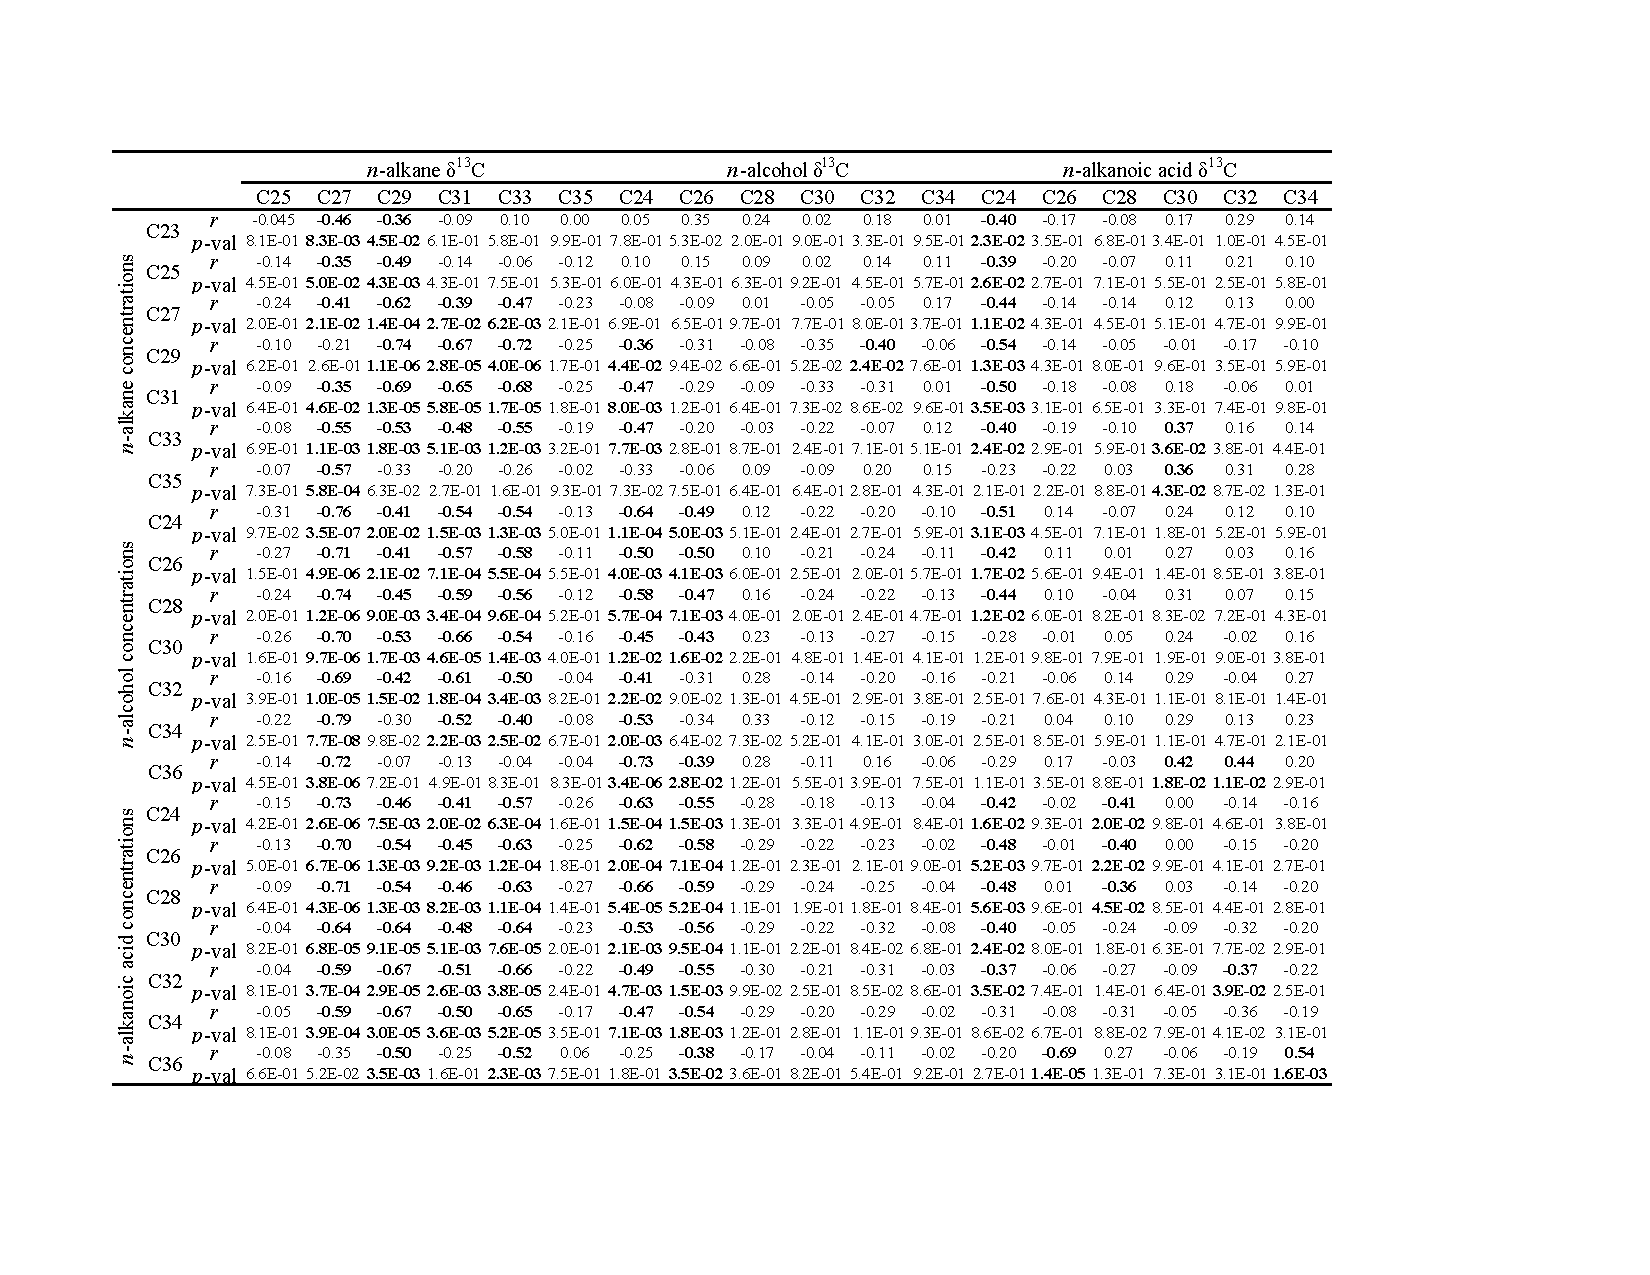
\includegraphics{Thesis_Tables/Ch4Tab3}
	\label{Ch4Tab:3} 
\end{sidewaystable}

\section{Discussion}

\subsection{\textit{n}-Alkane homologues variably record a spatially integrated signal}

Contrary to \textit{n}-alcohols and \textit{n}-alkanoic acids, Congo River carbon-normalized \textit{n}-alkane concentrations are relatively low compared to other large rivers studied \citep{vanDongen:2008kj,Galy:2011ix,Tao:2015bq}. In addition to vascular plants, petrogenic sources can also contribute to alkanes, especially even chain-length saturated homologues due to the low CPI value ($\approx 1.0$) of rock-derived sources as compared to plant waxes \citep{Eglinton:1967uz,Brooks:1969wh}. Low concentrations prevented the measurement of even chain-length \ce{\delta^{13}C} values in our samples, however CPI values between $2.1$ and $4.1$ indicate that \textit{n}-alkanes are dominated by a vascular plant signal. Additionally, the Congo catchment is composed mainly of Neoproterozoic craton lithology and exhibits low catchment relief, precluding a significant contribution of outcropped sedimentary rocks to Congo River suspended sediments \citep{Milliman:2011ug,Galy:2015fx}. Due to their lack of functional groups, \textit{n}-alkanes are more resistant to diagenetic degradation within soils and sediments than are \textit{n}-alkanoic acids and \textit{n}-alcohols \citep{Cranwell:1981vg,Meyers:1993up,Meyers:1993vwa, SinningheDamste:2002ud,vanDongen:2008kj}. For example, \citet{Hoefs:2002wu} show that \textit{n}-alkanes exhibit $\approx 3\times$ higher preservation factors than do \textit{n}-alkanoic acids upon re-exposure of anoxic sediments to oxygen, while \citet{Canuel:1996ta} and \citet{Sun:1994wj} calculate lower degradation rates for \textit{n}-alkanes than for functionalized lipids in both oxic and anoxic surface sediments. These results are consistent with observed pre-aging of \textit{n}-alkanes prior to fluvial export, as indicated by $^{14}$C-derived ages of plant-wax \textit{n}-alkanes in suspended sediments from other large rivers \citep[\textit{e.g.}][]{Gustafsson:2011ht,Tao:2015bq}.

Congo River suspended sediment \textit{n}-alkanes exhibit significantly lower CPI values than do \textit{n}-alcohols and \textit{n}-alkanoic acids (Figure \ref{Ch4Fig:5}C, \ref{Ch4Fig:5}F, \ref{Ch4Fig:5}I), suggesting increased exposure to diagenesis \citep{Meyers:1993vwa}. Additionally, a compilation of individual African forb, grass, shrub, and tree leaves indicates significant overlap in long-chain (\textit{i.e.} $\Sigma$LC\textsubscript{25-35}, $\Sigma$LC\textsubscript{26-36}) plant-wax concentrations and CPI values between compound classes (Table \ref{Ch4Tab:4}). We note that African plant \textit{n}-alkanoic acid concentration measurements are lacking ($n = 25$; Table \ref{Ch4Tab:4}), potentially leading to the higher mean and median values for this compound class. Inclusion of measurements from shrubs, grasses, and forbs raised in botanical gardens \citep{Gao:2014bk} lowers this mean value to $406$ $\mu$g g\textsuperscript{-1} dry leaf weight (inter-quartile range of $18 - 643$ $\mu$g g\textsuperscript{-1} dry leaf weight, $n = 72$), nearly identical to the mean of African plant \textit{n}-alkanes and \textit{n}-alcohols. Therefore, barring extreme biases against the transfer of plant-wax \textit{n}-alkanes into soils and subsequent entrainment into streams, their low and stable relative contribution to total \textit{n}-alkyl lipids in suspended sediments ($\leq 16$\%; Figure \ref{Ch4Fig:9}A, \ref{Ch4Fig:10}A) agrees with relatively stronger exposure to diagenesis as compared to \textit{n}-alcohols and \textit{n}-alkanoic acids.

% Table 4
\begin{sidewaystable}[p]
	\caption[Leaf lipid distributions and concentrations from African plants]{Summary statistics of plant-wax \textit{n}-alkane, \textit{n}-alcohol, and \textit{n}-alkanoic acid ($\Sigma$LC\textsubscript{25-35}, $\Sigma$LC\textsubscript{26-36}) concentration and CPI data from African plant leaves ($\mu$g g\textsuperscript{-1} dry leaf weight).}
	\centering
		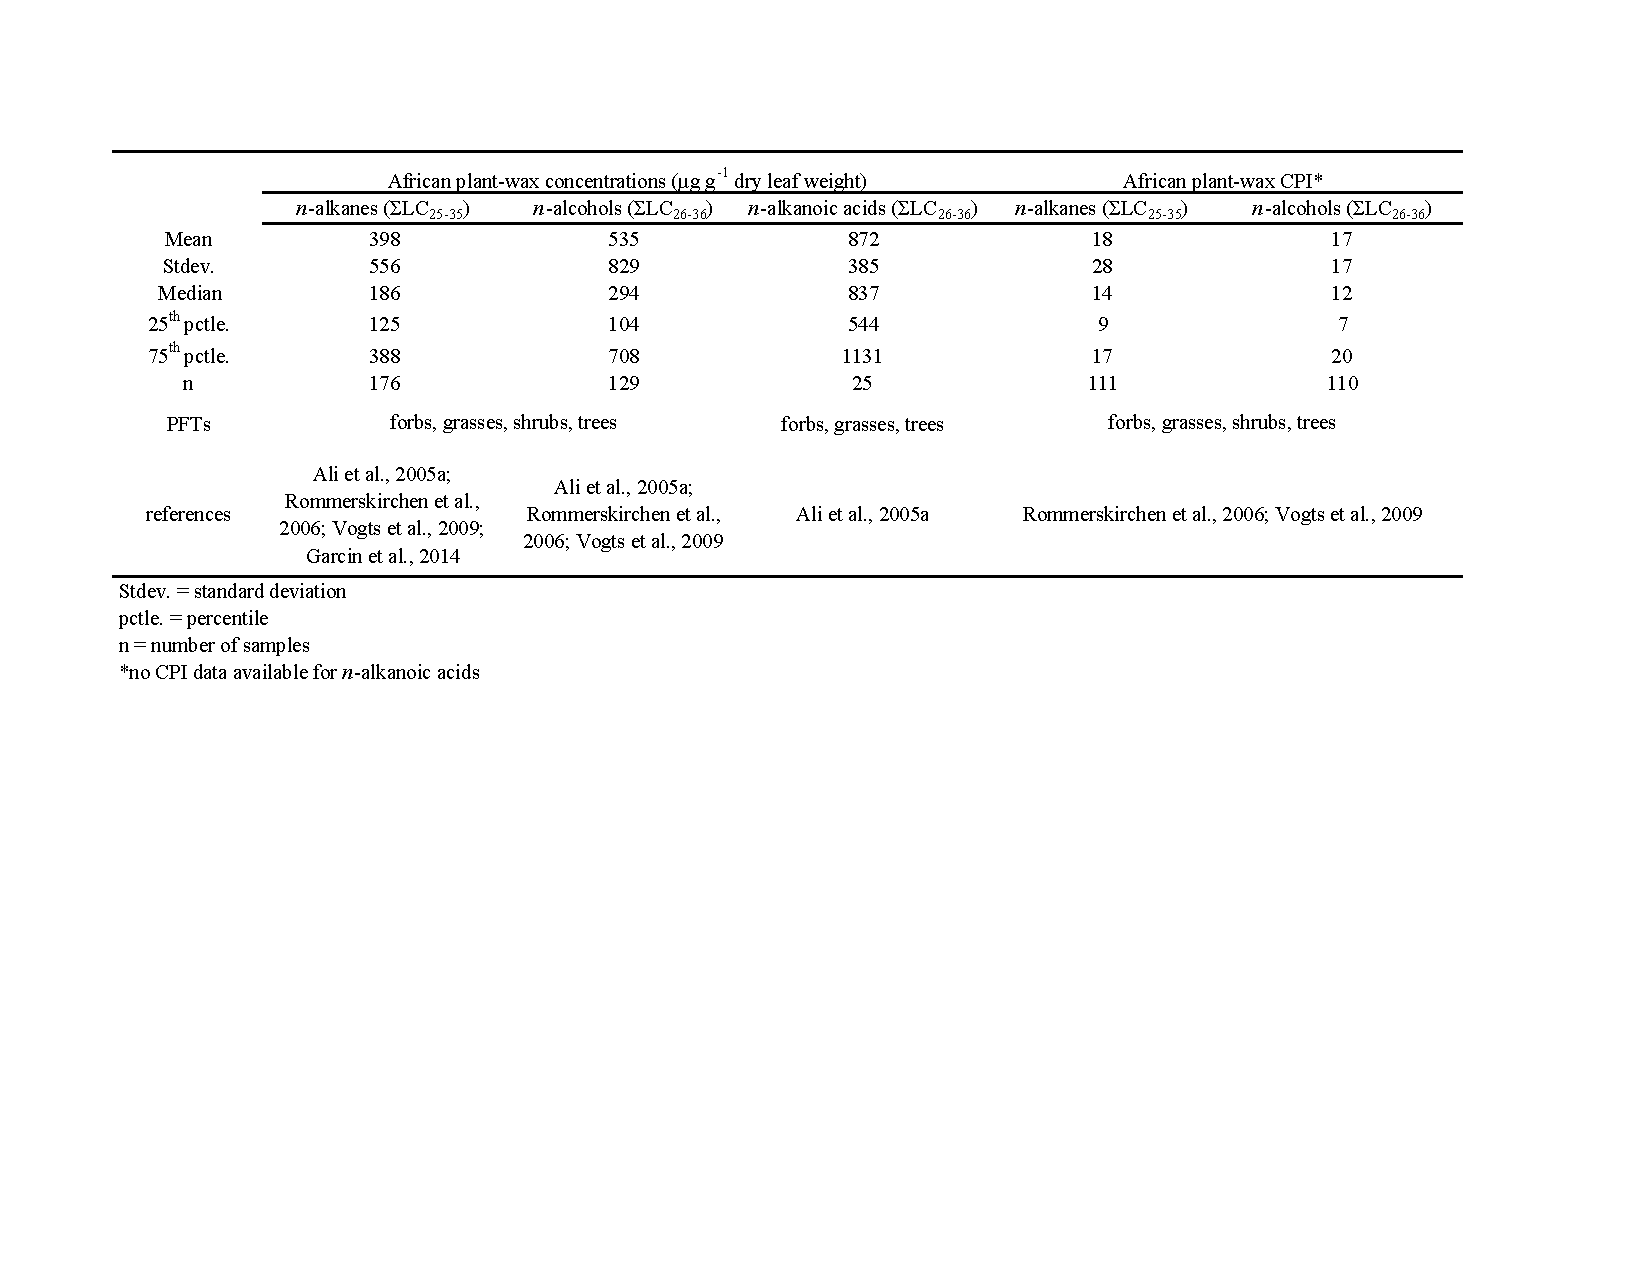
\includegraphics{Thesis_Tables/Ch4Tab4}
	\label{Ch4Tab:4} 
\end{sidewaystable}

% Figure 9
\begin{figure}[p]
	\makebox[\textwidth][c]{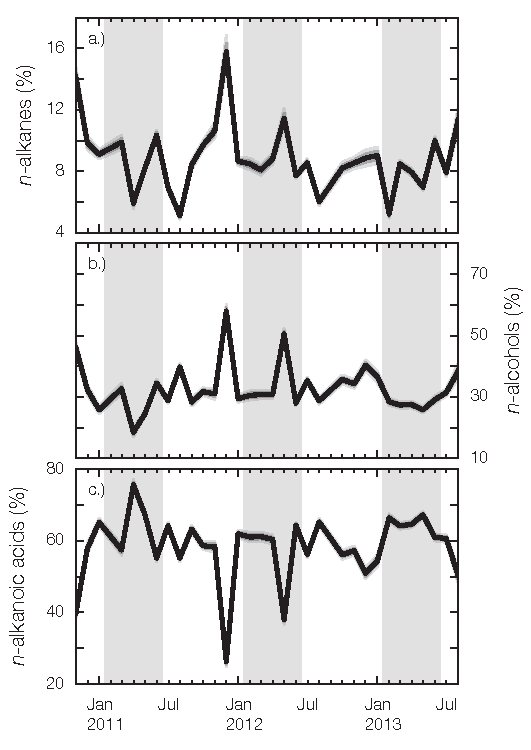
\includegraphics[]{Thesis_Figures/Ch4Fig9}}
	\caption[Time-series plots of compound-class contribution]{Time series plots of the fractional contribution to the plant-wax \textit{n}-alkyl lipid total by \textit{(A)} $\Sigma$LC\textsubscript{25-35} \textit{n}-alkanes, \textit{(B)} $\Sigma$LC\textsubscript{26-36} \textit{n}-alcohols, and \textit{(C)} $\Sigma$LC\textsubscript{26-36} \textit{n}-alkanoic acids. Dark gray shading represents $\pm 1 \sigma$ regression uncertainty, and light gray shading represents 95\% CI. Periods when f\textsubscript{south} > 39\% are indicated by gray boxes.}
	\label{Ch4Fig:9} 
\end{figure}

\textit{n}-Alkane concentrations, ACL, CPI, and \ce{\delta^{13}C} values show little to no correlation with discharge (Figure \ref{Ch4Fig:4}, \ref{Ch4Fig:5}A--C), indicating that exported \textit{n}-alkane signals do not respond to environmental changes on seasonal timescales. In contrast, if \textit{n}-alkanes were dominated by a recently entrained local signal, discharge should exhibit a strong control on molecular concentration/distribution and/or isotopic composition due to temporal variability in northern vs. southern hemisphere tributary contributions and their corresponding PFT signatures (Figure \ref{Ch4Fig:1}, \ref{Ch4Fig:2}B). However, this is not observed. This lack of correlation between \textit{n}-alkane concentration, ACL, and discharge likely explains the similarly low and invariant P\textsubscript{aq} values (Table \ref{Ch4Tab:S2}), as \textit{Cuvette Congolaise} macrophytes do not contribute significantly to exported \textit{n}-alkanes during periods of high northern hemisphere discharge.

Differences in isotope composition between homologues contain additional information related to residence time and end-member contribution in river systems with stable ecosystems and discharge source regions. Integration over multiple source regions with unique \textit{n}-alkane homologue distributions should result in large \ce{\delta^{13}C} variability with chain length. For example, \citet{Agrawal:2014fl} observed a consistent increase in \ce{\delta^{13}C} values with chain length of up to $\approx 6$\textperthousand\ between C\textsubscript{24} and C\textsubscript{32} \textit{n}-alkanoic acids in a sediment core taken from the Ganges floodplain at the base of the Himalayas. Additionally, they describe a unique "bimodal" concentration distribution with a maximum at C\textsubscript{24} and with significantly lower C\textsubscript{26}/C\textsubscript{28} and higher C\textsubscript{30}/C\textsubscript{32} concentrations than would be expected based on the distributions in modern Ganges suspended sediments \citep{Galy:2011ix}. Taken together, \citet{Agrawal:2014fl} use these results as evidence for degradation of Himalayan C\textsubscript{3} \textit{n}-alkanoic acids and replacement by local floodplain C\textsubscript{4}-derived compounds, and conclude that C\textsubscript{26}/C\textsubscript{28} better retain a headwater signal while C\textsubscript{30}/C\textsubscript{32} exhibit significant overprinting due to higher production of the longer-chain homologues by local C\textsubscript{4} grasses.

In the Congo River, integration of \textit{n}-alkanes over multiple source regions should result in a similarly large \ce{\delta^{13}C} difference across homologues and lower correlation between homologue concentrations, as is observed (Table \ref{Ch4Tab:1}; Figure \ref{Ch4Fig:3}D, \ref{Ch4Fig:4}D). Depleted \ce{\delta^{13}C} values for C\textsubscript{29} and C\textsubscript{31} \textit{n}-alkane confirm the importance of a C\textsubscript{3} source to these compounds, while relatively \ce{^{13}C}-enriched C\textsubscript{33} and, especially, C\textsubscript{35} values indicate a larger contribution by C\textsubscript{4} grasses with increasing chain length. This agrees with measurements of individual plant leaves, as African gramminoids have been shown to produce higher relative concentrations of C\textsubscript{33} (C\textsubscript{35} not measured) as compared to African trees and forbs \citep{Rommerskirchen:2006gr,Vogts:2009fb}. Using a typical end-member \textit{n}-alkane isotopic value of $-35$\textperthousand\ for C\textsubscript{3} and $-22$\textperthousand\ for C\textsubscript{4} plants \citep[\textit{e.g.}][]{Castaneda:2011jb}, this results in a C\textsubscript{4} contribution as high as $69 \pm 6$\% to C\textsubscript{35} \textit{n}-alkane and as low as $8 \pm 4$\% to C\textsubscript{29} \textit{n}-alkane, while remote-sensing results indicate that catchment-wide C\textsubscript{4} gramminoid coverage is $\approx 14$\% \citep[Figure \ref{Ch4Fig:1}B;][]{Still:2010wh}. However, we note that remote sensing likely underestimates C\textsubscript{4} coverage in forested areas, as C\textsubscript{4} plants are masked by C\textsubscript{3} forest canopy.

% Figure 10
\begin{figure}[p]
	\makebox[\textwidth][c]{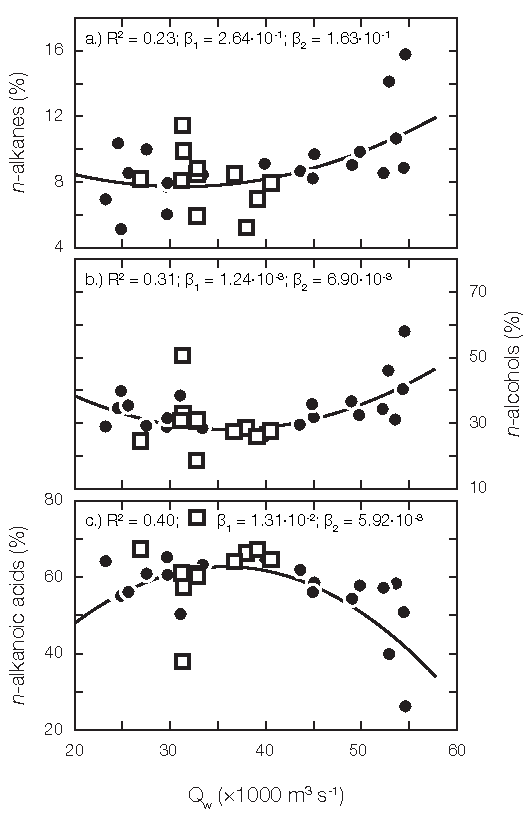
\includegraphics[]{Thesis_Figures/Ch4Fig10}}
	\caption[Correlation between compound-class contribution and discharge]{Fractional contribution by \textit{(A)} $\Sigma$LC\textsubscript{25-35} \textit{n}-alkanes, \textit{(B)} $\Sigma$LC\textsubscript{26-36} \textit{n}-alcohols, and \textit{(C)} $\Sigma$LC\textsubscript{26-36} \textit{n}-alkanoic acids plotted vs. Congo River discharge (Q\textsubscript{w}) measured at Brazzaville/Kinshasa. Black line is the quadratic WLS regression line. $R^2$ values and significance $p$-values for linear ($\beta_1$) and quadratic ($\beta_2$) parameters are reported for each regression. Samples collected when f\textsubscript{south} > 39\% are plotted as white squares, and samples collected when f\textsubscript{south} $\leq$ 39\% are plotted as black circles. Uncertainty ($\pm 1 \sigma$) is smaller than the symbols for all data points.}
	\label{Ch4Fig:10} 
\end{figure}

Spatially, C\textsubscript{4}-bearing savannah and woodland/shrubland ecosystems are mostly located at the northern and southern extremes of the catchment, above $5$\textdegree N and between $5-10$\textdegree S, while C\textsubscript{3}-dominated evergreen forest, deciduous/montane forest, and swamp forest occupy the central region (Figure \ref{Ch4Fig:1}). This geographic separation indicates a variable apparent integration region for \textit{n}-alkane homologues, with the longest chain-length \textit{n}-alkanes biasing toward headwater regions due to higher production by gramminoids. Additionally, observed negative correlations between C\textsubscript{27}--C\textsubscript{33} \textit{n}-alkane concentrations and \ce{\delta^{13}C} values (Table \ref{Ch4Tab:3}) are further evidence for an overprinting of distal C\textsubscript{4} sources during transit. This relationship is strongest for C\textsubscript{29} and C\textsubscript{31} ($r = -0.74$, $-0.65$), consistent with significant production of these compounds in C\textsubscript{3} trees and forbs \citep{Rommerskirchen:2006gr,Vogts:2009fb}. In contrast, C\textsubscript{35} \ce{\delta^{13}C} values are uncorrelated with concentration, further indicating a predominantly headwater C\textsubscript{4} source to this compound, irrespective of concentration. While regions of mosaic savannah/grassland and deciduous woodland/shrubland exist near the sampling site, especially in left-bank tributaries (Figure \ref{Ch4Fig:1}), this contribution is likely minimal. If local C\textsubscript{4} sources were important, this would lead to \ce{^{13}C}-enrichment of all \textit{n}-alkane homologues, especially during periods of predominantly southern hemisphere discharge, which is not observed (Figure \ref{Ch4Fig:4}D).

Biasing of C\textsubscript{33} and C\textsubscript{35} \textit{n}-alkanes toward a headwater C\textsubscript{4} signal agrees with time series measurements of the Oubangui River at Bangui Station ($4.36$\textdegree N, $18.55$\textdegree E; Figure \ref{Ch4Fig:1}). \citet{Bouillon:2012cw} show enriched POC \ce{\delta^{13}C} values ($-26.2 \pm 0.4$\textperthousand, $n = 11$) during periods of high discharge, when autochthonous production is negligible, as this headwater tributary contains significant amounts of dry woody savannah ecosystem coverage. Additionally, enriched POC \ce{\delta^{13}C} values up to $-22.8$\textperthousand\ have been reported for a small savannah tributary to the Oubangui River, while the nearby savannah-dominated Niari River exhibits POC \ce{\delta^{13}C} values as high as $-18.6$\textperthousand\ \citep{Mariotti:1991vx,Bouillon:2014ko}. In contrast, the Congo main-stem near Brazzaville displays more depleted POC \ce{\delta^{13}C} values, averaging $-28.2 \pm 0.4$\textperthousand\ \citep[$n = 5$;][]{Spencer:2012en}.

Additional evidence for variable spatial integration of \textit{n}-alkane homologues comes from a positive correlation between the \ce{\delta^{13}C} values of \textit{n}-alkanoic acids/\textit{n}-alcohols and their corresponding \textit{n}-alkanes (\textit{i.e.} $n - 1$), as decarboxylation and dehydration of functionalized \textit{n}-alkyl lipids has been shown to occur rapidly in sediments \citep{Cranwell:1981vg,Sun:1994wj,Sun:1997wr,Hoefs:2002wu}. Such relationships are especially strong between C\textsubscript{30}/C\textsubscript{32} \textit{n}-alcohol and \textit{n}-alkanoic acid and C\textsubscript{29}/C\textsubscript{31} \textit{n}-alkane ($r$ up to $0.75$; Table \ref{Ch4Tab:2}), indicating that diagenetic contribution by functionalized C\textsubscript{3} plant waxes contributes to the overprinting of these compounds during transit. Taken together, the observed depleted \ce{\delta^{13}C} values, negative correlations between \ce{\delta^{13}C} and concentration, and positive \ce{\delta^{13}C} correlations with corresponding functionalized lipids indicate that C\textsubscript{29} and C\textsubscript{31} \textit{n}-alkane exhibit significant overprinting during fluvial transit and bias toward a more local signal. In contrast, enriched \ce{\delta^{13}C} values and weaker correlation between \ce{\delta^{13}C} and concentration for C\textsubscript{33} and, especially, C\textsubscript{35} \textit{n}-alkanes are strong evidence that these homologues better retain a headwater signal.

\subsection{\textit{n}-Alcohols and \textit{n}-alkanoic acids are controlled by recently entrained local sources}\label{Ch4Sec:52}

Contrary to \textit{n}-alkanes, carbon-normalized concentrations of plant-wax \textit{n}-alcohols and \textit{n}-alkanoic acids in Congo River POC are equal to or greater than the highest observed values in any large river system to date \citep{Saliot:2001un,vanDongen:2008kj,Galy:2011ix,Tao:2015bq}. Such high \textit{n}-alcohol:\textit{n}-alkane ($3.8 \pm 0.9$) and \textit{n}-alkanoic acid:\textit{n}-alkane ($7.1 \pm 2.5$) ratios in suspended sediments contrast with the overlapping range in concentrations between compound classes found in African plants (Table \ref{Ch4Tab:4}). Additionally, despite an identical range in CPI for \textit{n}-alkanes and \textit{n}-alcohols (no \textit{n}-alkanoic data exist) in individual African plant leaves (Table  \ref{Ch4Tab:4}), both functionalized compound classes exhibit higher CPI values than do \textit{n}-alkanes in suspended sediment (Tables \ref{Ch4Tab:S2}--\ref{Ch4Tab:S4}), as diagenetic degradation has been shown to lower CPI \citep{Meyers:1993vwa}.

Assuming no pervasive biases against the transfer of \textit{n}-alkanes into soils and subsequent entrainment into streams, high concentrations and CPI values of functionalized lipids relative to \textit{n}-alkanes, despite similar input composition from plants (Table \ref{Ch4Tab:4}), supports the hypothesis that exported \textit{n}-alcohols and \textit{n}-alkanoic acids are mostly sourced from local surface soils with less exposure to diagenesis prior to export. Functionalized wax lipids are known to experience rapid diagenetic dehydration and decarboxylation in sediments \citep{Meyers:1993up,Sun:1994wj,Canuel:1996ta,Sun:1997wr}. For example, \citet{Sun:1997wr} report that 90\% of $^{14}$C-labeled C\textsubscript{16} \textit{n}-alkanoic acids (labeled in the methyl position) are degraded due to decarboxylation within 80 days during incubation experiments. While C\textsubscript{16} \textit{n}-alkanoic acid is produced ubiquitously in the environment, rapid degradation has additionally been observed for plant-wax-specific \textit{n}-alkanoic acids (\textit{i.e.} C\textsubscript{26}--C\textsubscript{30}) and \textit{n}-alcohols (C\textsubscript{26}--C\textsubscript{30}) upon re-exposure of sediments to oxygen \citep{Hoefs:2002wu}. \textit{n}-Alkanoic acids and \textit{n}-alcohols frequently exhibit the lowest preservation of all lipids in marine and lacustrine sediments and have been observed to degrade at faster rates than bulk OC \citep{Cranwell:1981vg,Meyers:1993vwa}. However, lipid preservation is additionally a function of sediment mineralogy, as sorptive interactions with mineral surfaces have been shown to stabilize labile OC \citep[\textit{e.g.}][]{Keil:1994hb,Mayer:1994wn}.

Isotopic evidence further indicates a predominantly local source, as these compound classes exhibit depleted \ce{\delta^{13}C} values for all plant-wax homologues (average $\leq -31.3$\textperthousand\ and $-30.8$\textperthousand, respectively; Figure \ref{Ch4Fig:3}E--F). Using a C\textsubscript{3} end-member value of -35\textperthousand\ and a C\textsubscript{4} end-member value of -22\textperthousand, as above \citep{Castaneda:2011jb}, this leads to a minimum C\textsubscript{3} contribution to \textit{n}-alcohols of $73 \pm 5$\% (C\textsubscript{32}) and $68 \pm 6$\% to \textit{n}-alkanoic acids (C\textsubscript{26}). However, this is likely an underestimate, as relatively enriched \ce{\delta^{13}C} values for individual C\textsubscript{3} angiosperm lipids have been reported \citep[\textit{i.e.} up to $-30$\textperthousand; ][]{Diefendorf:2011hg,Garcin:2014hg}. Isotopic evidence therefore indicates that functionalized lipids are predominantly sourced from local C\textsubscript{3} ecosystems, as C\textsubscript{4} land cover is mostly limited to distal headwater regions (Figure \ref{Ch4Fig:1}B). Similar to \textit{n}-alkanes, regions of mosaic savannah/grassland and deciduous woodland/shrubland near the sampling site likely do not contribute significantly to exported \textit{n}-alcohols and \textit{n}-alkanoic acids, as this would lead to a \ce{^{13}C}-enrichment during southern hemisphere dominated discharge periods, which is not observed (Figure \ref{Ch4Fig:6}D, \ref{Ch4Fig:7}D, \ref{Ch4Fig:8}).

Unlike longer chain homologues, autochthonous production of C\textsubscript{24} \textit{n}-alcohol has been observed in freshwater phytoplankton \citep{Volkman:1998tk,Volkman:1999tq,Xu:2007jk}, and is likely a significant source of this compound in our sample set. This is supported by depleted \ce{\delta^{13}C} values (Figure \ref{Ch4Fig:3}E) and a strong positive relationship with discharge (Figure \ref{Ch4Fig:8}A). 

If dissolved inorganic carbon (DIC) is \ce{^{13}C}-depleted relative to atmospheric \ce{CO2}, autochthonous contribution will lead to lower observed \ce{\delta^{13}C} values for C\textsubscript{24} \textit{n}-alcohol, especially during periods of low discharge when phytoplankton production is highest. While no DIC \ce{\delta^{13}C} values exist at our sampling site, low- and rising-water values at Bangui station average $-10.0 \pm 2.2$\textperthousand\ \citep[$n = 30$;][]{Bouillon:2012cw,Bouillon:2014ko}.  Additionally, C\textsubscript{24} \textit{n}-alcohol \ce{\delta^{13}C} values are strongly correlated with those of C\textsubscript{22} \textit{n}-alcohol ($R^2 = 0.75$, $p$-value = $4.0 \times 10^{-10}$; not shown), the dominant lipid in freshwater phytoplankton \citep{Volkman:1998tk,Volkman:1999tq,Xu:2007jk}, and are uncorrelated with longer chain-length values ($p$-value > $0.05$; not shown). While a slight \ce{\delta^{13}C} vs. discharge correlation is observed for other compounds (\textit{i.e.} C\textsubscript{26} \textit{n}-alcohol, C\textsubscript{24} and C\textsubscript{28} \textit{n}-alkanoic acid; Figure \ref{Ch4Fig:8}), these homologues are consistently $\approx 3-5$\textperthousand\ enriched relative to C\textsubscript{24} \textit{n}-alcohol, indicating minimal autochthonous contribution.

Further evidence for a local, C\textsubscript{3} signal to functionalized \textit{n}-alkyl lipids comes from the fact that \ce{\delta^{13}C} values show significantly weaker negative correlation with lipid concentrations than do \textit{n}-alkanes, with the exception of C\textsubscript{24} \textit{n}-alcohol and C\textsubscript{24} \textit{n}-alkanoic acid (Table \ref{Ch4Tab:3}). As with \textit{n}-alkanes, a negative correlation would indicate addition of C\textsubscript{3} material to a background C\textsubscript{4} signal during transit. However, this is not the case, especially for longer chain-length homologues (\textit{i.e.} C\textsubscript{28+}), indicating negligible contribution by C\textsubscript{4}-dominated headwater ecosystems to measured compounds and therefore a smaller apparent integration region than is observed for \textit{n}-alkanes, especially C\textsubscript{33} and C\textsubscript{35}. African C\textsubscript{4} gramminoids exhibit similar \textit{n}-alcohol and \textit{n}-alkanoic acid production rates as African forbs, shrubs, and trees \citep{Ali:2005ab,Rommerskirchen:2006gr,Vogts:2009fb}, indicating that this signal is not due to a source effect. Rather, it is likely the result of quantitative diagenetic degradation of headwater functionalized \textit{n}-alkyl lipids during fluvial transit \citep{Cranwell:1981vg,Meyers:1993vwa,Sun:1997wr,Hoefs:2002wu,vanDongen:2008kj}. In addition, a low spread in \ce{\delta^{13}C} values across plant-wax chain-lengths (Figure \ref{Ch4Fig:3}E--F) and strong positive correlations between homologue concentrations (Table \ref{Ch4Tab:1}) precludes significant spatial integration of multiple PFTs with unique molecular distribution and isotope composition \citep[\textit{c.f.}][]{Agrawal:2014fl}.

Additionally, we observe large seasonal variability in \textit{n}-alcohol and \textit{n}-alkanoic acid relative contribution (Figure \ref{Ch4Fig:9}), indicating a change in functionalized lipid source in response to seasonal hydrology. This is consistent with the above evidence that these compounds are sourced from recently entrained OC and integrate a mostly local signal. \textit{n}-Alcohol relative contribution displays a statistically significant increase during \textit{Cuvette Congolaise} dominated periods, balanced by an equal decrease in \textit{n}-alkanoic acids (Figure \ref{Ch4Fig:10}). These results agree with literature measurements of individual plants, as macrophytes display considerably higher \textit{n}-alcohol production rates than do other PFTs \citep{Ficken:1998vs,Ficken:2000wq,Bugalho:2004kj,Ali:2005ab,Ali:2005cr,Aichner:2010bk,Gao:2011dj,Diefendorf:2011hg,Wang:2012fb,Gao:2014bk}.

It has been shown that the Congo main-stem and a range of tributaries bias toward swamp-forest-like chemical properties during periods of high discharge, indicating an increased contribution by this ecosystem to exported organic carbon \citep{Wang:2013js,Mann:2014jx}. These observations, combined with an increase in \textit{n}-alcohol fractional contribution, are strong evidence for a significant increase in \textit{Cuvette Congolaise} contribution to functionalized \textit{n}-alkyl lipids during periods of high northern hemisphere discharge. Thus, our results indicate that this geographically small region \citep[4\% coverage;][]{Mayaux:2004uw} exhibits a dominant control on the composition of exported functionalized \textit{n}-alkyl lipids in response to seasonal changes in hydrology. However, a lack of significant \ce{\delta^{13}C} variability across the time series for any functionalized plant-wax lipid (Figure \ref{Ch4Fig:6}D, \ref{Ch4Fig:7}D) indicates that their \ce{\delta^{13}C} values are not a sensitive tracer for changes in \textit{n}-alkyl lipid source on these timescales.

\subsection{Comparison to other river basins and global significance}

Variable spatiotemporal integration of \textit{n}-alkane homologues and a local, recently entrained \textit{n}-alcohol/\textit{n}-alkanoic acid signal is a feature not limited to the Congo River catchment. For example, isotopic and molecular signals of \textit{n}-alkanes and \textit{n}-alkanoic acids show differential contribution by C\textsubscript{4} grasses during transport in the Ganges River through the floodplain \citep{Galy:2011ix}. Using the data of \citet{Galy:2011ix}, we compare the concentration-weighted Himalayan plant-wax signal to that just before the confluence with the Brahmaputra River in Bangladesh, noting that sediment fluxes are nearly identical in all major Himalayan tributaries \citep{Andermann:2012br}.

Himalayan plant-wax \textit{n}-alkanes (C\textsubscript{25}--C\textsubscript{35}) and \textit{n}-alkanoic acids (C\textsubscript{26}--C\textsubscript{34}) display nearly identical \ce{\delta^{13}C} composition, averaging $-32.1$\textperthousand\ and $-32.3$\textperthousand\ respectively, with similar spread between chain-lengths of $1.8$\textperthousand\ and $1.4$\textperthousand. In contrast, downstream Ganges \textit{n}-alkanoic acid \ce{\delta^{13}C} values are enriched by an average of $1.3$\textperthousand\ relative to \textit{n}-alkanes. Additionally, isotopic spread between chain lengths remains constant for \textit{n}-alkanoic acids (\textit{i.e.} $1.4$\textperthousand), but increases to $3.5$\textperthousand\ for \textit{n}-alkanes, while ACL of both compound classes increases by $\approx 1$ unit. Combined, these results indicate that C\textsubscript{3} \textit{n}-alkanoic acids sourced in the Himalayan range are quantitatively replaced by a mixed C\textsubscript{3}/C\textsubscript{4} floodplain signal independent of chain length. In contrast, \textit{n}-alkanes display differential contribution by a floodplain signal across chain lengths, with C\textsubscript{33}/C\textsubscript{35} showing the most influence. Quantitative \textit{n}-alkanoic acid replacement during floodplain transit agrees with the results of \citet{Agrawal:2014fl}, which already show significant overprinting near the base of the Himalayan range. Thus, despite large differences in sediment erosion rates and biospheric carbon yields between the Congo and Ganges rivers \citep{Galy:2015fx}, exported plant waxes display similar behavior in these two catchments.

In addition to the Ganges River, a large spread in \textit{n}-alkane \ce{\delta^{13}C} values with chain-length has been observed in settings such as Cameroonian lacustrine and Washington margin surface sediments \citep{Feng:2013iv,Garcin:2014hg} and a Zambezi River sedimentary archive \citep{Wang:2013jz}. Differential contribution by C\textsubscript{3}/C\textsubscript{4} plants to \textit{n}-alkanes with chain length therefore appears to be a common phenomenon. We suggest that \ce{\delta^{13}C} measurement of multiple \textit{n}-alkane chain lengths can be used to address nonlinear PFT mixing during transport \citep{Garcin:2014hg}, as C\textsubscript{33} and, especially, C\textsubscript{35} bias almost exclusively toward a C\textsubscript{4} end-member, opposite to C\textsubscript{29} and C\textsubscript{31}.

Additionally, differential sourcing between compound classes (\textit{i.e.} functionalized vs. \textit{n}-alkanes) appears to be common in river catchments spanning multiple ecosystems. Thus, in addition to \textit{n}-alkanes, measurement of \textit{n}-alcohols and \textit{n}-alkanoic acids in river sediments and fluvially dominated sedimentary archives can be utilized to address geospatial PFT distribution within the catchment, as functionalized lipids will bias toward a local signal \citep[\textit{e.g.}][this study]{Galy:2011ix,Ponton:2014jr}.

\section{Conclusion}

We report concentrations and \ce{\delta^{13}C} values of three classes of dominantly plant-derived \textit{n}-alkyl lipids from a 34-month time series of Congo River suspended sediments. Our results show that \textit{n}-alkanoic acid and \textit{n}-alcohol concentrations are equal to or greater than the highest OC-normalized concentrations in large fluvial systems reported to date. In contrast, \textit{n}-alkanes concentrations are lower than those reported in other major rivers. Spread in \textit{n}-alcohol and \textit{n}-alkanoic acid \ce{\delta^{13}C} values between long-chain homologues is lower than observed in other major rivers, while \textit{n}-alkanes exhibit up to $\approx 8$\textperthousand\ enrichment with increasing chain length.

These data indicate that \textit{n}-alkanoic acids and \textit{n}-alcohols are sourced from local, C\textsubscript{3}-dominated ecosystems, consistent with the idea that high reactivity of functional groups precludes significant spatial integration of these compounds. In contrast, \textit{n}-alkane homologues variably integrate over a wide range of ecosystems with increasing contribution by distal C\textsubscript{4}-dominated savannah and woodland/shrubland source regions to the longest chain-length compounds. Strong seasonal shifts in relative \textit{n}-alkanoic acid and \textit{n}-alcohol concentrations indicate that functionalized lipids respond rapidly to changes in hydrological regime. This signal, however, is not reflected in \ce{\delta^{13}C} values. During periods of highest northern hemisphere discharge, an increase in fractional \textit{n}-alcohol contribution and decrease in \textit{n}-alkanoic acid contribution suggest a strong bias towards a local swamp-forest signal. \textit{n}-Alkanes are less affected by seasonal changes in discharge, further indicating that these compounds integrate over a larger source region.

Consequently, we suggest that simultaneous measurement of multiple \textit{n}-alkyl lipid classes and chain lengths in down-core samples will likely provide better geospatial resolution for paleo-ecosystem reconstruction due to their differential integration regions and C\textsubscript{3}/C\textsubscript{4} biases.

%\section*{Acknowledgements}

%We thank Carl Johnson (WHOI), Sarah Rosengard (WHOI), and Ralph Kreutz (MARUM) for laboratory assistance. V.V.G. was partly supported by the US National Science Foundation, grants OCE-0851015 and OCE-0928582; J.D.H. was supported by the National Science Foundation Graduate Research Fellowship under Grant No. 2012126152; E.S was supported by the DFG Research Center/Cluster of Excellence "The Ocean in the Earth System" at MARUM -- Center for Marine Environmental Science, University of Bremen. This manuscript benefited greatly through the constructive comments of Aaron Diefendorf, Clayton Magill, one anonymous reviewer, and associate editor Thomas Bianchi.

\clearpage

\section{Supplementary Material}

\subsection{Supplementary Tables}

% Reset table counter
\renewcommand\thetable{\thechapter.S\arabic{table}}    
\setcounter{table}{0}

% Change caption justification
\captionsetup[table]{justification=raggedright,singlelinecheck=off}

All supplementary tables for this chapter are available in the open-source \emph{Pangaea} database at the following link: \url{https://doi.pangaea.de/10.1594/PANGAEA.864152}

% Table S1
\begin{table}[h!]
	\caption[Congo River environmental parameters]{Environmental parameters for the Congo River recorded near Brazzaville/Kinshasa during the sampling period (November 2010 -- August 2013).}
	\label{Ch4Tab:S1} 
\end{table}

% Table S2
\begin{table}[h!]
	\caption[\textit{n}-alkane concentrations, ACL, CPI, and P\textsubscript{aq}]{Concentrations of \textit{n}-alkanes, average chain length, and carbon preference index during the sampling period (November 2010 -- August 2013).}
	\label{Ch4Tab:S2} 
\end{table}

% Table S3
\begin{table}[h!]
	\caption[\textit{n}-alcohol concentrations, ACL, and CPI]{Concentrations of \textit{n}-alcohols, average chain length, and carbon preference index during the sampling period (November 2010 -- August 2013).}
	\label{Ch4Tab:S3} 
\end{table}

% Table S4
\begin{table}[h!]
	\caption[\textit{n}-alkanoic acid concentrations, ACL, and CPI]{Concentrations of \textit{n}-alkanoic acids, average chain length, and carbon preference index during the sampling period (November 2010 -- August 2013).}
	\label{Ch4Tab:S4} 
\end{table}

% Table S5
\begin{table}[h!]
	\caption[\textit{n}-alkane \ce{\delta^{13}C} values]{\ce{\delta^{13}C} values of \textit{n}-alkanes during the sampling period (November 2010 -- August 2013).}
	\label{Ch4Tab:S5} 
\end{table}

% Table S6
\begin{table}[h!]
	\caption[\textit{n}-alcohol \ce{\delta^{13}C} values]{\ce{\delta^{13}C} values of \textit{n}-alcohols during the sampling period (November 2010 -- August 2013).}
	\label{Ch4Tab:S6} 
\end{table}

% Table S7
\begin{table}[h!]
	\caption[\textit{n}-alkanoic acid \ce{\delta^{13}C} values]{\ce{\delta^{13}C} values of \textit{n}-alkanoic acids during the sampling period (November 2010 -- August 2013).}
	\label{Ch4Tab:S7} 
\end{table}

% Table S8
\begin{table}[h!]
	\caption[Compound class relative contributions]{Relative compound class contributions to total \textit{n}-alkyl lipids during the sampling period (November 2010 -- August 2013).}
	\label{Ch4Tab:S8} 
\end{table}

% Reset for future chapters
\renewcommand\thetable{\thechapter.\arabic{table}}

% Reset caption justification
\captionsetup[table]{justification=justified}
   

% Chapter 5 text
\chapter{Hydrologic controls on the seasonal and inter-annual variability in Congo River particulate organic carbon sources and reservoir age}
\label{Ch5}
\raggedbottom

{\let\thefootnote\relax\footnotetext{This chapter is currently in preparation for submission as: Hemingway J.D., Schefu\ss \ E., Spencer R.G.M., Dinga B.J., Eglinton T.I., McIntyre C., and Galy V.V. {Hydrologic controls on the seasonal and inter-annual variability in Congo River particulate organic carbon and GDGT sources.}}}

\clearpage

\section{Abstract}

Tropical rivers are a major source of organic matter (OM) to the coastal ocean and play a large role in the global carbon cycle. As such, it is critical to understand the sources, sinks, and transformations of OM during fluvial transit over seasonal and inter-annual timescales. Here we present dissolved organic carbon (DOC) concentrations, particulate OM (POM) composition (\ce{\delta^{13}C}, \ce{\delta^{15}N}, \ce{\Delta^{14}C}, N/C), and glycerol dialkyl glycerol tetraether (GDGT) biomarker distributions from a 34-month time-series near the mouth of the Congo River.

An end-member mixing model based on \ce{\delta^{13}C} and N/C indicates that exported POM is consistently dominated by C\textsubscript{3} tropical rainforest soil inputs, with increasing contributions by C\textsubscript{3} tropical plant vegetation and decreasing contributions by autochthonous phytoplankton at high discharge. Inputs from C\textsubscript{4} plants and soils are negligible throughout the time-series despite covering $\approx 13$\% of the catchment. Calculated \ce{\Delta^{14}C} values of the C\textsubscript{3}-soil end member reveal significant and variable pre-aging prior to export, especially during the year 2011 when southern-hemisphere discharge reached record lows (mean = $-176$\textperthousand, standard deviation = $93$\textperthousand). In contrast, soil \ce{\Delta^{14}C} values were stable near $-50$\textperthousand\ between January and June 2013 when southern-hemisphere discharge was highest. These results indicate that headwater POM is diluted and/or overprinted by C\textsubscript{3} vegetation and pre-aged soils during transit through the \textit{Cuvette Congolaise} swamp forest, while left-bank tributaries export significantly less pre-aged material.

Glycerol dialkyl glycerol tetraether (GDGT) biomarker distributions provide further evidence for changes in soil provenance, as branched and isoprenoid GDGT distributions both exhibit large seasonal and inter-annual variability. Methylation and cyclization of branched tetraethers (MBT', CBT) and the GDGT-0/crenarchaeol ratio (GDGT-0/cren) are positively correlated with discharge ($r \geq 0.62$; $p$-value $\leq 1.39 \times 10^{-4}$) and reflect a significant incorporation of compounds produced in permanently inundated \textit{Cuvette Congolaise} swamp-forest soils, especially in 2011, thus highlighting the importance of this region in controlling organic carbon export.

\section{Introduction}

River networks act as a dynamic link between terrestrial and aquatic ecosystems and play a major role in the global carbon cycle via the weathering of silicate minerals \citep{Berner:1983uk,Gaillardet:1999uy}, oxidation of rock-derived organic carbon \citep[OC\textsubscript{petro};][]{Galy:2008ff,Bouchez:2010if,Hilton:2014dh}, and export of biospheric particulate OC (POC) to the coastal ocean coupled with subsequent burial in marine sediments \citep{Berner:1982vg,Galy:2007ev}. Additionally, because POC buried in large fluvial fans is typically thought to integrate over a wide geographic area, paleo-environmental proxies such as bulk \ce{\delta^{13}C}, plant-wax \ce{\delta^{13}C}, and glycerol dialkyl glycerol tetraether (GDGT) molecular distributions in sedimentary archives are commonly used to reconstruct past ecosystem coverage and environmental conditions \citep[\textit{e.g.}][]{FranceLanord:1994vp,Freeman:2001tv,Schefuss:2005jo,Weijers:2007fp}.

There has thus been a significant effort to determine the geologic and climatic controls on the source, composition, and export flux of biospheric POC in modern rivers across the globe due to the fact that burial of this material in marine sediments constitutes a net atmospheric \ce{CO2} sink \citep{Lasaga:1985ts,Ludwig:1996ul,Galy:2015fx}. Furthermore, it is now known that rivers are generally not passive conduits to the ocean, but rather integrate, process, and remineralize multiple sources of terrestrial (allochthonous) and aquatic (autochthonous) organic matter (OM) during transit \citep{Cole:2007gp,Aufdenkampe:2011fm}. For example, \citet{Galy:2008jw,Galy:2011ix} analyzed the \ce{^{13}C} composition of bulk POC and plant-wax \textit{n}-alkanoic acids in Ganges-Brahmaputra suspended sediments to conclude that headwater Himalayan C\textsubscript{3} material is replaced by a floodplain-derived mixed C\textsubscript{3}/C\textsubscript{4} signal prior to export. Similarly, downstream decreases in bulk \ce{^{13}C} composition and carbon-normalized lignin concentration have been observed in Amazon River fine-grained POC and are attributed to the addition of floodplain soil material \citep{Hedges:1986ab,Hedges:2000tn}.

Specific to the Congo Basin, recent studies based on the isotope composition of dissolved lithium and silicon suggest that "black water" rivers such as those draining the permanently inundated \textit{Cuvette Congolaise} swamp forest (Figure \ref{Ch5Fig:1}A) contribute $\approx 30$\% of the water discharged at Brazzaville/Kinshasa annually, with significantly higher contributions during peak discharge \citep{Cardinal:2010ir,Henchiri:2016jh}. However, the mechanisms controlling the influence of this end member on exported suspended sediments in general and particulate OM (POM) in particular remain unknown \citep{Spencer:2016ho}.

% Figure 1
\begin{figure}[ht]
	\makebox[\textwidth][c]{\includegraphics[]{Thesis_Figures/Ch5Fig1}}
	\caption[Congo catchment map showing landcover and \%C\textsubscript{3} vs. \%C\textsubscript{4} vegatation]{Congo, Djoue, and Oubangui catchment outlines showing $(A)$ ecosystem landcover \citep{Mayaux:2004uw} and $(B)$ C\textsubscript{3}/C\textsubscript{4} landcover \citep{Still:2010wh}. Our sampling location is marked as a red circle (this marker covers both the Congo and Djoue River sampling sites), while Bangui Station \citep{Bouillon:2012cw,Bouillon:2014ko} is marked as a white diamond. Djoue and Oubangui River sub-basins upstream of each sampling location are highlighted in pastel colors.}
	\label{Ch5Fig:1} 
\end{figure}

Still, \citet{Laraque:2009fz} observe a decrease in sediment yield downstream of the \textit{Cuvette Congolaise} as compared to upstream tributaries, suggesting that a significant amount of headwater material can settle out during passage through this central depression. Exported sediments are therefore biased downstream, as evidenced by the \ce{^{13}C} and molecular composition of exported plant-wax \textit{n}-alcohols and \textit{n}-alkanoic acids, which are consistently dominated by a swamp-forest-derived C\textsubscript{3} signal during periods of high discharge \citep{Hemingway:2016bq}. Furthermore, millennial-scale changes in climate and hydrology likely influence the ability of the \textit{Cuvette Congolaise} to act as an OM reservoir and POM source. For example, \citet{Schefuss:2016cp} show that the terrestrial reservoir age of exported plant waxes has been steadily increasing since the humid Early- to Mid-Holocene ($\approx$10,000--5,000 years before present), suggesting that pre-aged \textit{Cuvette}-derived OM is remobilized during periods of decreased rainfall in the basin.

Despite these findings, quantitatively partitioning POM sources and understanding the mechanisms that control their variability on seasonal and inter-annual timescales remains an open question in the Congo River system. To estimate POM source contributions, multiple (pseudo-)conservative tracers such as \ce{\delta^{13}C}, \ce{\Delta^{14}C}, and the N/C ratio are frequently used in end-member mixing models \citep{Perdue:2007fn,Weijers:2009iu,Hilton:2010cg,Hossler:2012jh}, although this requires that end-member compositions are well-constrained and can lead to spurious results if temporal variability in such composition is unknown. Still, this method has been successfully utilized to separate OM sources in riverine suspended sediments \citep{Hilton:2010cg,Hossler:2012jh} and to calculate terrestrial contribution to continental shelf sediments \citep{Gordon:2004id,Weijers:2009iu}. 

In addition to bulk measurements, microbial GDGT membrane lipids can offer further insight as a tracer for OM sources. The concentrations and molecular compositions of both branched (brGDGTs) and isoprenoid (isoGDGTs) GDGTs have become a commonly used proxy to determine the source of POM in a host of environments and to record environmental conditions such as temperature and soil pH \citep[see][for review]{Castaneda:2011jb,Schouten:2013bd}. For example, because brGDGTs are thought to be produced predominantly in soils while isoGDGTs are dominant in aquatic environments, the branched to isoprenoid tetraether (BIT) index first described by \citet{Hopmans:2004kx} is often used in fluvial suspended sediments \citep{Kim:2012fq,Zell:2014gt}, lacustrine sediments \citep{Tierney:2010br}, and continental shelf sediments \citep{Peterse:2009hl,Weijers:2009iu} to estimate soil OM contribution. Furthermore, the methylation of branched tetraether (MBT') and cyclization of branched tetraether (CBT) indices have been shown to co-vary with temperature and pH in a global soil dataset \citep{Weijers:2007gu,Peterse:2012bs,DeJonge:2014kw} and have thus been utilized in large fluvial catchments as a tracer of OC source \citep{Zell:2013eg,DeJonge:2014fs}. Because the Congo River covers multiple ecosystems that are described by a range of environmental conditions such as soil pH \citep{Mayaux:2004uw,Spencer:2012en}, GDGT signals should provide an additional constraint on exported POM provenance.

Combined, bulk POM and GDGT temporal and spatial variability imply that POM and biomarker geographic integration in large river systems is non-uniform and that exported signals are likely subject to large seasonal/inter-annual changes in end-member contribution \citep[\textit{e.g.}][]{Galy:2008jw,Zell:2013eg,Spencer:2016ho}. To understand this variability in the Congo basin, we extend published records of Congo River main-stem OM \citep{Mariotti:1991vx,Coynel:2005cn,Spencer:2012en,Hemingway:2016bq,Spencer:2016ho} by reporting dissolved organic carbon (DOC) concentrations, POM composition (\ce{\delta^{13}C}, \ce{\delta^{15}N}, \ce{\Delta^{14}C}, N/C), and GDGT distributions from a 34-month time-series collected at Brazzaville/Kinshasa (see Table \ref{Ch5Tab:1}; Figure \ref{Ch5Fig:1} for sampling locations). Additionally, we present bulk POM measurements (\ce{\delta^{13}C}, \ce{\delta^{15}N}, N/C) from the Djoue River, a small mixed C\textsubscript{3}/C\textsubscript{4} end-member tributary near Brazzaville, for a 13-month subset of this time-series. Combined with a previously published 2-year time-series from the Oubangui River upstream of the \textit{Cuvette Congolaise}  \citep{Bouillon:2012cw,Bouillon:2014ko}, our results thus provide an understanding of POM source evolution during fluvial transit through this permanently inundated swamp forest. Lastly, we discuss the influence of climate and hydrology on the \textit{Cuvette Congolaise} as a POM source both on inter-annual timescales and with respect to paleo-environmental records derived from the Congo Fan.

% Table 1
\begin{table}[ht]
	\caption[Congo, Djoue, and Oubangui catchment properties and landcover composition]{Congo, Djoue, and Oubangui catchment properties and landcover composition.}
	\makebox[\textwidth][c]{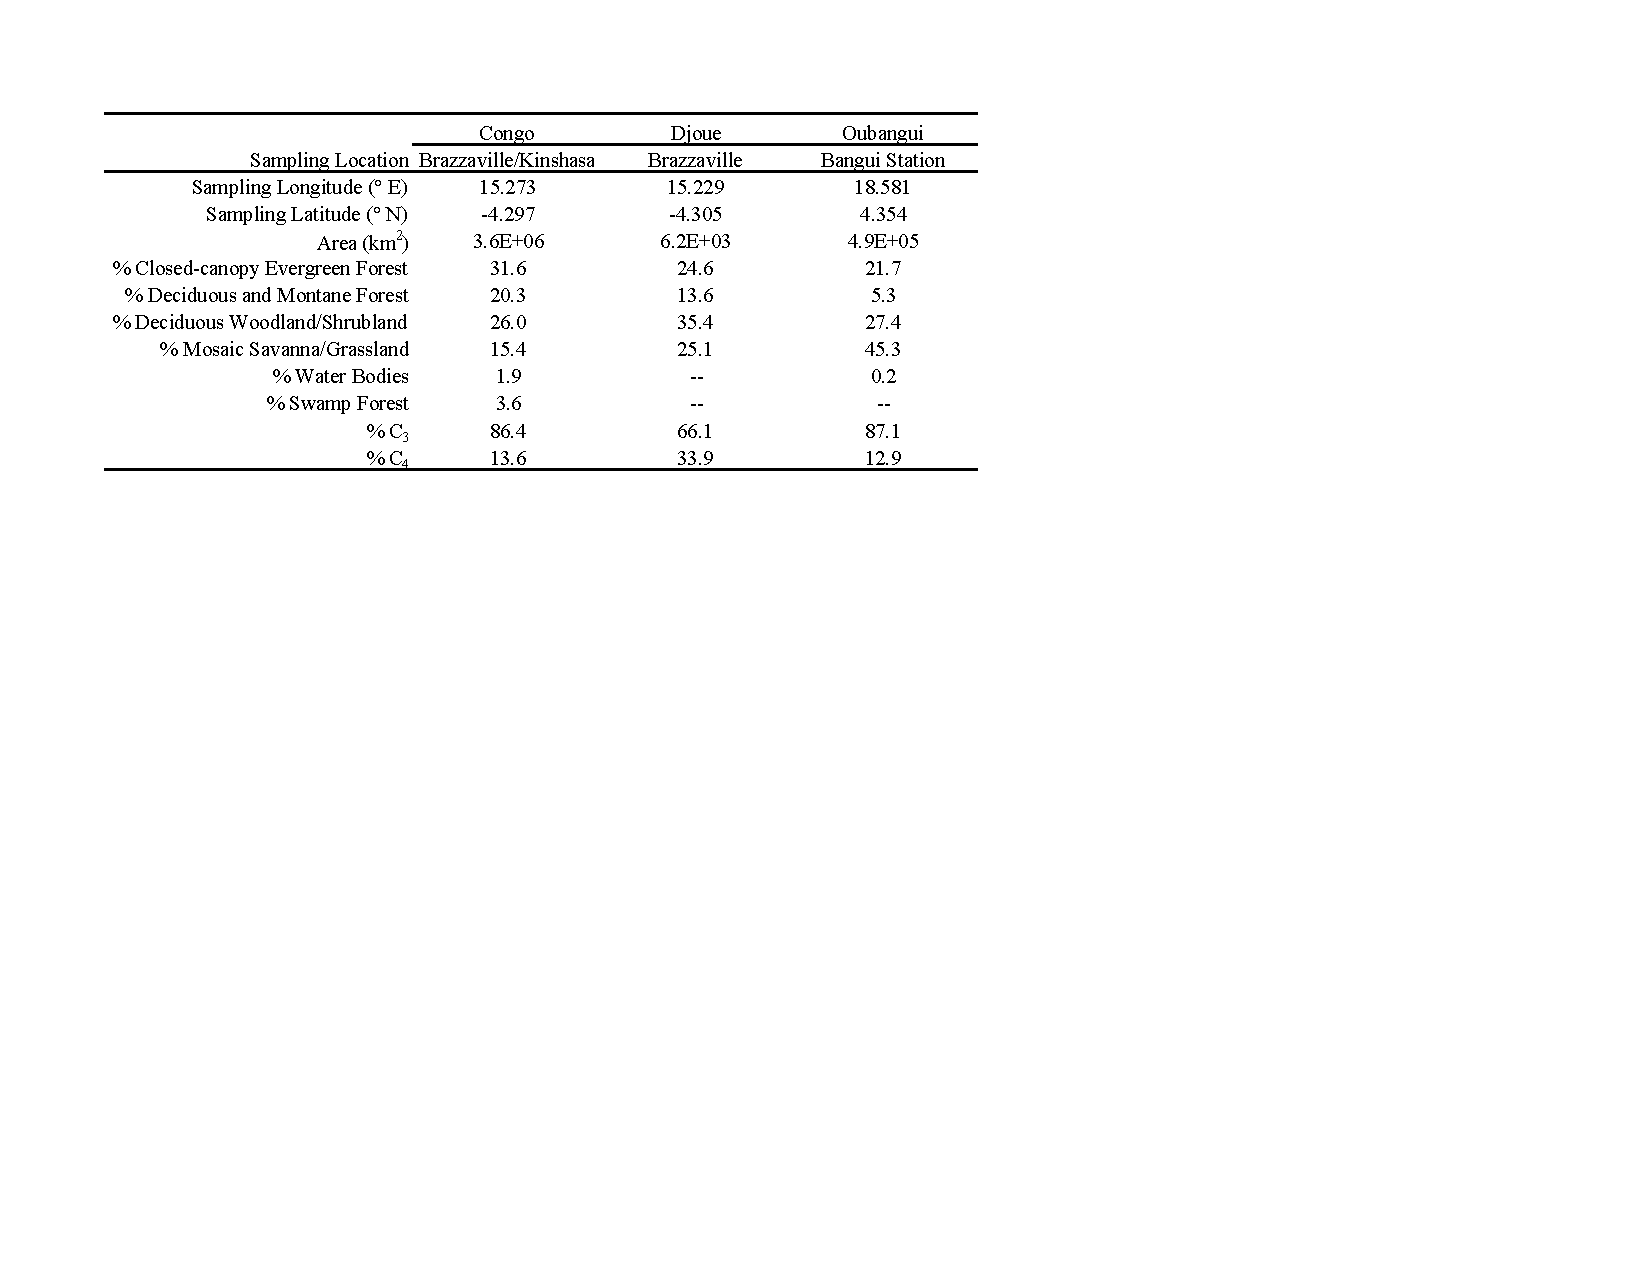
\includegraphics[]{Thesis_Tables/Ch5Tab1}}
	\label{Ch5Tab:1} 
\end{table}

\section{Study Site}

The Congo River drains $3.6 \times 10^6$ km\textsuperscript{2} of central Africa between $10$\textdegree N and $15$\textdegree S and is highly influenced by the seasonal north-to-south migration of the inter-tropical convergence zone \citep[ITCZ;][]{Gasse:2000ul}. This leads to strong latitudinal gradients in vegetation and ecosystem type \citep{Mayaux:2004uw}, including the \textit{Cuvette Congolaise} swamp forest (Figure \ref{Ch5Fig:1}A), and corresponding changes in C\textsubscript{3} vs. C\textsubscript{4} landcover \citep[Figure \ref{Ch5Fig:1}B;][]{Still:2010wh}. The Congo basin is dominated by closed-canopy evergreen forest near the equator and deciduous woodland/shrubland at the northern and southern peripheries, with smaller contributions by deciduous and montane forests, mosaic savanna/grassland, and swamp forest (Table \ref{Ch5Tab:1}). In contrast, both the Oubangui sub-basin upstream of Bangui Station and the Djoue River contain mostly mosaic savannah/grassland and deciduous woodland/shrubland. This leads to $\geq 85$\% C\textsubscript{3} landcover in the Congo and Oubangui basins, while the Djoue exhibits more evenly mixed C\textsubscript{3}/C\textsubscript{4} coverage (Table \ref{Ch5Tab:1}).

Congo River discharge (Q\textsubscript{w}) recorded at Brazzaville/Kinshasa is remarkably stable and predictable, with an annual maximum near $50,000$ m\textsuperscript{3} s\textsuperscript{-1} and a minimum near $25,000$ m\textsuperscript{3} s\textsuperscript{-1} \citep[Figure \ref{Ch5Fig:2}A;][]{Coynel:2005cn,Laraque:2009fz,Spencer:2014vp}. Increased precipitation in the north of the catchment between May and September \citep{Mahe:1993wu} and a $\approx 1 - 2$ month transit time \citep{Bricquet:1993ve} leads to discharge maxima of right-bank (\textit{i.e.} northern-hemisphere) tributaries such as the Oubangui River during Nov-Dec-Jan \citep{Coynel:2005cn,Bouillon:2012cw,Bouillon:2014ko} and corresponds to elevated water flux through the \textit{Cuvette Congolaise} during this time. Between November and March, southern-hemisphere precipitation increases left-bank tributary contribution in response to the seasonal ITCZ migration and is the source of the secondary discharge maximum observed during Apr-May-Jun \citep[Figure \ref{Ch5Fig:2}A;][]{Bricquet:1993ve,Mahe:1993wu}. Importantly, the largest left-bank tributary (Kasai River) enters the main-stem downstream of the \textit{Cuvette Congolaise}. In contrast to the Congo River main-stem, Oubangui River discharge is highly seasonal, ranging from $\approx 300$ m\textsuperscript{3} s\textsuperscript{-1} in Mar-Apr-May to $\approx 9,000$ m\textsuperscript{3} s\textsuperscript{-1} in Oct-Nov-Dec \citep{Bouillon:2012cw,Bouillon:2014ko}.

% Figure 2
\begin{figure}[p]
	\makebox[\textwidth][c]{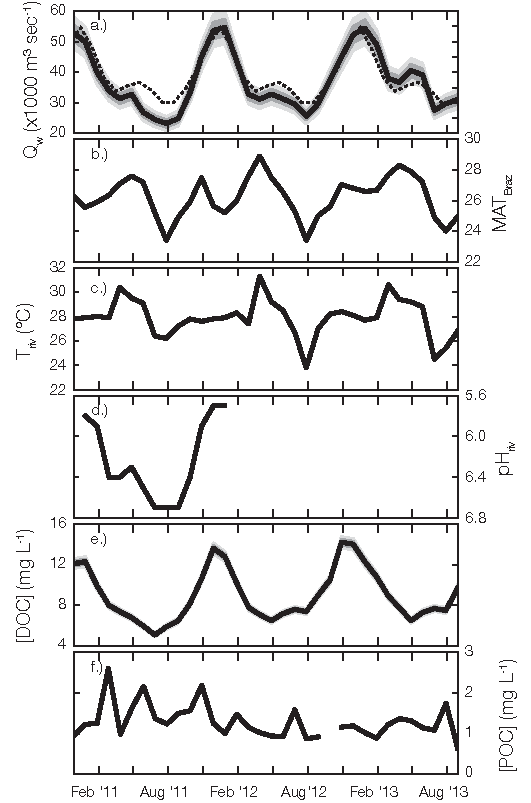
\includegraphics[]{Thesis_Figures/Ch5Fig2}}
	\caption[Environmental parameter time-series plots]{Time-series plots of Congo River $(A)$ discharge (Q\textsubscript{w}), $(B)$ mean monthly air temperature at Brazzaville/Kinshasa (MAT\textsubscript{Braz}), $(C)$ measured river water temperature (T\textsubscript{riv}), $(D)$ measured river water pH from \citet{Wang:2013js} (pH\textsubscript{riv}), $(E)$ DOC concentration ([DOC]), and $(F)$ POC concentration ([POC]) from \citet{Hemingway:2016bq}. Where visible, dark gray envelope is $\pm 1 \sigma$ uncertainty and light gray envelope is 95\% confidence interval. Dotted line in panel $(A)$ is the 1977--2006 (inclusive) average hydrograph \citep{Spencer:2012en}.}
	\label{Ch5Fig:2} 
\end{figure}

\section{Materials and Methods}

\subsection{Sample collection}

Congo River samples were collected monthly between November 2010 and August 2013 near Brazzaville/Kinshasa, just downstream of the Pool Malebo and $\approx 300$ km upstream of the Congo Estuary (Table \ref{Ch5Tab:1}; Figure \ref{Ch5Fig:1}), while Djoue River samples were similarly collected between November 2010 and November 2011. The Congo River sampling location is downstream of all major tributaries, capturing $>95$\% of the total catchment \citep{Spencer:2012en}. Water for total suspended sediments (TSS) was collected from the surface of the river and filtered through $0.22 \mu$m polyether sulfone (PES) membrane filters. After drying ($60$\textdegree C) and shipment, samples were re-suspended in $18$M$\Omega$ Milli-Q water, freeze-dried, and weighed for TSS concentration. Simultaneously, Congo River water was collected for DOC analysis and filtered through $0.7 \mu$m pre-combusted ($550$\textdegree C, 4 hours) GF/F filters into acid pre-leached and triple sample-rinsed HDPE bottles. DOC samples were acidified to pH $2$ using trace-metal grade HCl and immediately frozen until further analysis.

Surface water temperatures (T\textsubscript{riv}) were measured concurrently using a YSI Professional Plus multiparameter instrument (YSI Incorporated) and daily Congo River discharge was measured at a nearby gauging station operated by the Institute de Recherche en Sciences Exactes et Naturelles (Republic of Congo) using a rating curve that is periodically updated by Acoustic Doppler Current Profiler (ADCP) transects. Triplicate ADCP transects suggest that river discharge measurements are precise to $\pm 5$\%, although precision is likely lower during high discharge due to overbank flooding \citep{Spencer:2014vp}. Monthly mean air temperature recorded at Brazzaville/Kinshasa (MAT\textsubscript{Braz}; $4.25$\textdegree S, $15.25$\textdegree E) was obtained from the National Oceanic and Atmospheric Administration (NOAA) National Climate Data Center database. MAT was missing for one month (April 2012) and was therefore estimated as the average between mean daily maximum and minimum temperatures during that month. 

\subsection{Bulk measurements}

DOC concentration ([DOC]) was quantified via high-temperature combustion using a Shimadzu TOC-V organic carbon analyzer. Each sample was injected until there existed triplicate measurements with a coefficient of variability $\leq 2$\%, and was calibrated to a six-point calibration curve after accounting for instrument drift using an internal control standard following \citet{Mann:2012kp}. [DOC] is taken as the mean of these triplicate values with a relative uncertainty ($\pm 1 \sigma$) of $\pm 2$\%.

Organic carbon and nitrogen percentages (\%OC, \%N\textsubscript{org}) and stable isotopes (\ce{\delta^{13}C}, \ce{\delta^{15}N}) were measured on TSS aliquots following the methods of \citet{Whiteside:2011jea}. We note that one sample (September 2012) became contaminated by dissolution of the PES membrane during re-suspension and was therefore omitted from bulk measurements. All other samples were acidified under HCl fumes at $60$\textdegree C for 72 hours to remove carbonates prior to \%OC and \ce{\delta^{13}C} measurement using a Fisons elemental analyzer coupled to a Finnigan Delta\textsuperscript{plus} isotope-ratio mass spectrometer (IRMS). \%N\textsubscript{org} and \ce{\delta^{15}N} measurements were performed similarly but using non-acidified aliquots. All samples were injected in triplicate and calibrated against \ce{CO2} or \ce{N2} gas with known isotope composition. Uncertainty is taken as the standard deviation of triplicate measurements and isotope values are reported as per-mille (\textperthousand) deviations from Vienna Pee Dee Belemnite (VPDB) for \ce{\delta^{13}C} and atmospheric \ce{N2} (AIR) for \ce{\delta^{15}N}.

Aliquots for radiocarbon analysis, along with corresponding process blanks and standards, were subjected to the acidification treatment described above and were oxidized to \ce{CO2} by baking ($850$\textdegree C, 5 hours) with $\approx 1$ g cupric oxide in evacuated and flame-sealed quartz tubes. \ce{CO2} gas was then distilled cryogenically, transferred to Pyrex tubes, and analyzed for radiocarbon content using a mini carbon dating system (MICADAS) accelerator mass spectrometer fitted with a gas-ion source (Ionplus AG) at the Laboratory for Ion Beam Physics, ETH Zurich \citep{Christl:2013ks}. Data are corrected for process blanks and reported following the \ce{\Delta^{14}C} per-mille notation of \citet{Stuiver:1977uh}.

\subsection{GDGT extraction and purification}

Remaining Congo River TSS was extracted at $100$\textdegree C for 20 minutes in a microwave accelerated reaction system (MARS, CEM Corporation) in $20$ mL of dichloromethane (DCM) and methanol (9:1). Because \textit{n}-alkyl lipid isotopes were also measured on these samples \citep{Hemingway:2016bq}, total lipid extracts were saponified at $70$\textdegree C for 2 hours using $0.5$ M KOH in methanol. GDGT distributions reported here therefore represent a combination of core lipids and intact polar phospholipids, as base hydrolysis is known to cleave phosphate-bound head groups \citep{Weijers:2011bn}.

Subsequently, $15$ mL of $18$M$\Omega$ Milli-Q water was added and "base" fractions were liquid-liquid extracted into $5$ mL hexane 5 times. HCl was then added drop-wise until pH $2$ was reached, and "acid" fractions were extracted using 5mL hexane and DCM (4:1) until the organic phase was clear (typically 5 times). Acid and base fractions were separated by column chromatography using $1$ g of Supelclean amino-propyl silica gel (Supelco Analytical) and the following elution scheme: $4$ mL hexane (F1); $7$ mL hexane and DCM (4:1, F2); $10$ mL DCM and acetone (9:1, F3); $14$ mL 2\% (w/w) formic acid in DCM (F4); $18$ mL DCM and methanol (1:1, F5). Acid and base fractions containing GDGTs (F3) were recombined to ensure maximum recovery. To remove \textit{n}-alcohols, combined F3s were subjected to urea adduction in which $500 \mu$L of urea-saturated methanol was added and solvent was evaporated using a stream of \ce{N2} gas to promote urea recrystallization (repeated three times). Crystals were rinsed three times with $5$ mL hexane to remove the "non adducted" fraction containing GDGTs, which was then stored at $4$\textdegree C until analysis. While the additional handling steps described here likely lower GDGT recovery, results from a recent inter-comparison exercise \citep{Schouten:2013hh} indicate that our purification protocol does not impart a significant bias in GDGT distributions as compared to other commonly used methods \citep[\textit{e.g.} the modified Bligh and Dyer method of][]{Pitcher:2009jd}.

\subsection{GDGT detection and analysis}

GDGTs were detected on an Agilent 1200 series high-pressure liquid chromatograph coupled to an Agilent LC/MSD SL quadrupole mass spectrometer (HPLC-MS) as initially described by \citet{Hopmans:2000ti}. Compounds were ionized using atmospheric-pressure chemical ionization (APCI) and detected on their [M+H]\textsuperscript{+} ions in selected ion monitoring (SIM) mode. Chromatographic separation was achieved in normal phase through a Grace Prevail Cyano $3 \mu$m column ($150$ mm $\times$ $2.1$ mm). Samples were injected ($5 \mu$L) and solvent A (99:1 [v/v] hexane:isopropanol) was pumped at $0.2$ mL/min isocratically for 5 minutes, then with a linear gradient for 40 minutes, reaching 10\% solvent B (9:1 [v/v] hexane:isopropanol). We note that this chromatographic method cannot separate multiple co-eluting compounds such as the six distinct peaks at $1050$ m/z observed by \citet{Becker:2013jw} and the recently discovered 6-methyl brGDGTs IIa'--IIIc' \citep[see Figure \ref{Ch5Fig:S1} for structures;][]{DeJonge:2013cr,DeJonge:2014kw}. Such co-elution could potentially alter calculated brGDGT metrics, although this effect is likely negligible in our sample set (see Supplemental Discussion \ref{Ch5SD1}).

A laboratory working standard was injected at multiple concentrations between every 5--10 samples ($n = 32$) and showed $<10$\% variability for all metrics over all concentrations throughout the analysis, indicating minimal instrument drift. Metrics and ratios were calculated based on raw areas (\textit{i.e.} molar ratios), assuming an identical response factor of all isoGDGTs and brGDGTs in accordance with current best practice \citep{Schouten:2013hh,Schouten:2013bd}. Metrics were calculated following the equations of \citet{Hopmans:2004kx}, \citet{Peterse:2012bs}, and \citet{Weijers:2007gu}, respectively:

% Equation 1
\begin{equation}\label{Ch5Eq:1}
	\text{BIT} = \frac{\{\text{brIa}\} + \{\text{brIIa}\} + \{\text{brIIIa}\}}{\{\text{brIa}\} + \{\text{brIIa}\} + \{\text{brIIIa}\} + \{\text{cren}\}}
\end{equation}

% Equation 2
\begin{equation}\label{Ch5Eq:2}
	\text{MBT'} = \frac{\{\text{brIa}\} + \{\text{brIb}\} + \{\text{brIc}\}}{\{\text{brIa}\} + \{\text{brIb}\} + \{\text{brIc}\} + \{\text{brIIa}\} + \{\text{brIIb}\} + \{\text{brIIc}\} + \{\text{brIIIa}\}}
\end{equation}

% Equation 3
\begin{equation}\label{Ch5Eq:3}
	\text{CBT} = -\log \frac{\{\text{brIb}\} + \{\text{brIb}\}}{\{\text{brIa}\} + \{\text{brIIa}\}}
\end{equation}

where $\{j\}$ is the area of the [M+H]\textsuperscript{+} ion for compound $j$, noting that $\{\text{brIIa}\} - \{\text{brIIIa}\}$ represent the sum of co-eluting 5-methyl and 6-methyl compounds \citep{DeJonge:2014kw}. Additionally, the GDGT-0/cren was calculated as $\{\text{GDGT-0}\}/\{\text{cren}\}$ following \citet{Blaga:2009ge}. All samples were injected in triplicate and metrics are reported as the mean and standard deviation of triplicate measurements.

\subsection{Data analysis and model setup}

All regressions were performed as ordinary least squares (OLS) and statistical results are reported as regression coefficients ($r$) and significance $p$-values. Time-series average values are reported as the mean $\pm 1$ standard deviation about the mean. All data analysis was performed in the Python programming language v.2.7 and ArcGIS for Desktop v.10.3.

Quantitative contribution of $m$ end members to bulk POM was determined following optimum multi-parameter analysis (OMPA) using $m-1$ (pseudo-)conservative tracers, as described in \citet{Glover:2011uh}. End-member composition uncertainty was incorporated by \textit{(i)} including a weighting factor for each tracer equal to the range of observed values divided by the average end-member uncertainty and \textit{(ii)} allowing for 1\% deviation in the constraint that fractional contributions sum to unity \citep{Glover:2011uh}. Additionally, because phytoplankton \ce{\delta^{13}C} is known to vary seasonally in the Congo basin \citep{Bouillon:2014ko}, the composition of this end member was allowed to vary and the model was re-initialized for each sample.

To determine the environmental controls on GDGT metrics, redundancy analysis (RDA) was performed following \citet{Legendre:1998tt}. In the resulting triplot, the "site" and "species" scores were scaled symmetrically by the square root of corresponding eigenvalues ("Type III" scaling).

\section{Results}

All environmental parameters and bulk measurements are reported in Table \ref{Ch5Tab:S1} while all GDGT fractional abundances and calculated metrics are reported in Table \ref{Ch5Tab:S2}. 

\subsection{Environmental parameters}

Congo River discharge recorded at Brazzaville/Kinshasa during the time-series ranged from $(23.2 \pm 1.1) \times 10^3$ m\textsuperscript{3} s\textsuperscript{-1} in July 2011 to $(54.6 \pm 2.7) \times 10^3$ m\textsuperscript{3} s\textsuperscript{-1} in December 2011 (Figure \ref{Ch5Fig:2}A). Annual averaged discharge for 2012 and 2013 is near the long-term mean value of $38.8 \times 10^3$ m\textsuperscript{3} s\textsuperscript{-1} (1977--2006 inclusive), however average discharge for 2011 ($35.3 \times 10^3$ m\textsuperscript{3} s\textsuperscript{-1}) is the fifth-lowest in this record \citep{Spencer:2012en}. Importantly, this is due to a significantly suppressed left-bank discharge maximum during Apr-May-Jun as compared to the 1977--2006 mean for these months. In contrast, northern-hemisphere peak discharge (Nov-Dec-Jan) is near the long-term average for all years in the time-series presented here (Figure \ref{Ch5Fig:2}A).

MAT\textsubscript{Braz} correlates strongly with T\textsubscript{riv} (Table \ref{Ch5Tab:2}) and both are relatively invariable over the time-series (Figure \ref{Ch5Fig:2}B, \ref{Ch5Fig:2}C). T\textsubscript{riv} ranges from a minimum of $23.8$\textdegree C to a maximum of $31.3$\textdegree C (mean = $27.9 \pm 1.6$\textdegree C), while MAT\textsubscript{Braz} exhibits similar values, ranging from $23.4$\textdegree C to $28.9$\textdegree C (mean = $26.2 \pm 1.3$\textdegree C). Both T\textsubscript{riv} and MAT\textsubscript{Braz} are uncorrelated with all other environmental parameters, bulk POM measurements, and GDGT metrics. In contrast, pH\textsubscript{riv} is strongly correlated with Q\textsubscript{w} over the 13-month subset of the time-series in which data exist \citep[$r = -0.97$, $p$-value = $1.25 \times 10^{-8}$;][]{Wang:2013js}, and ranges from a minimum of $5.7$ units to a maximum of $6.7$ units (mean = $6.2 \pm 0.4$; Figure \ref{Ch5Fig:2}D).

% Table 2
\begin{sidewaystable}[p]
	\caption[Environmental parameter, POM, and GDGT correlation coefficients]{Matrix of correlation coefficients ($r$) and significance $p$-values for Congo River environmental parameters, POM composition, and GDGT distribution metrics. Statistically significant ($p$-value $\leq 0.05$) correlations are bolded.}
	\centering
		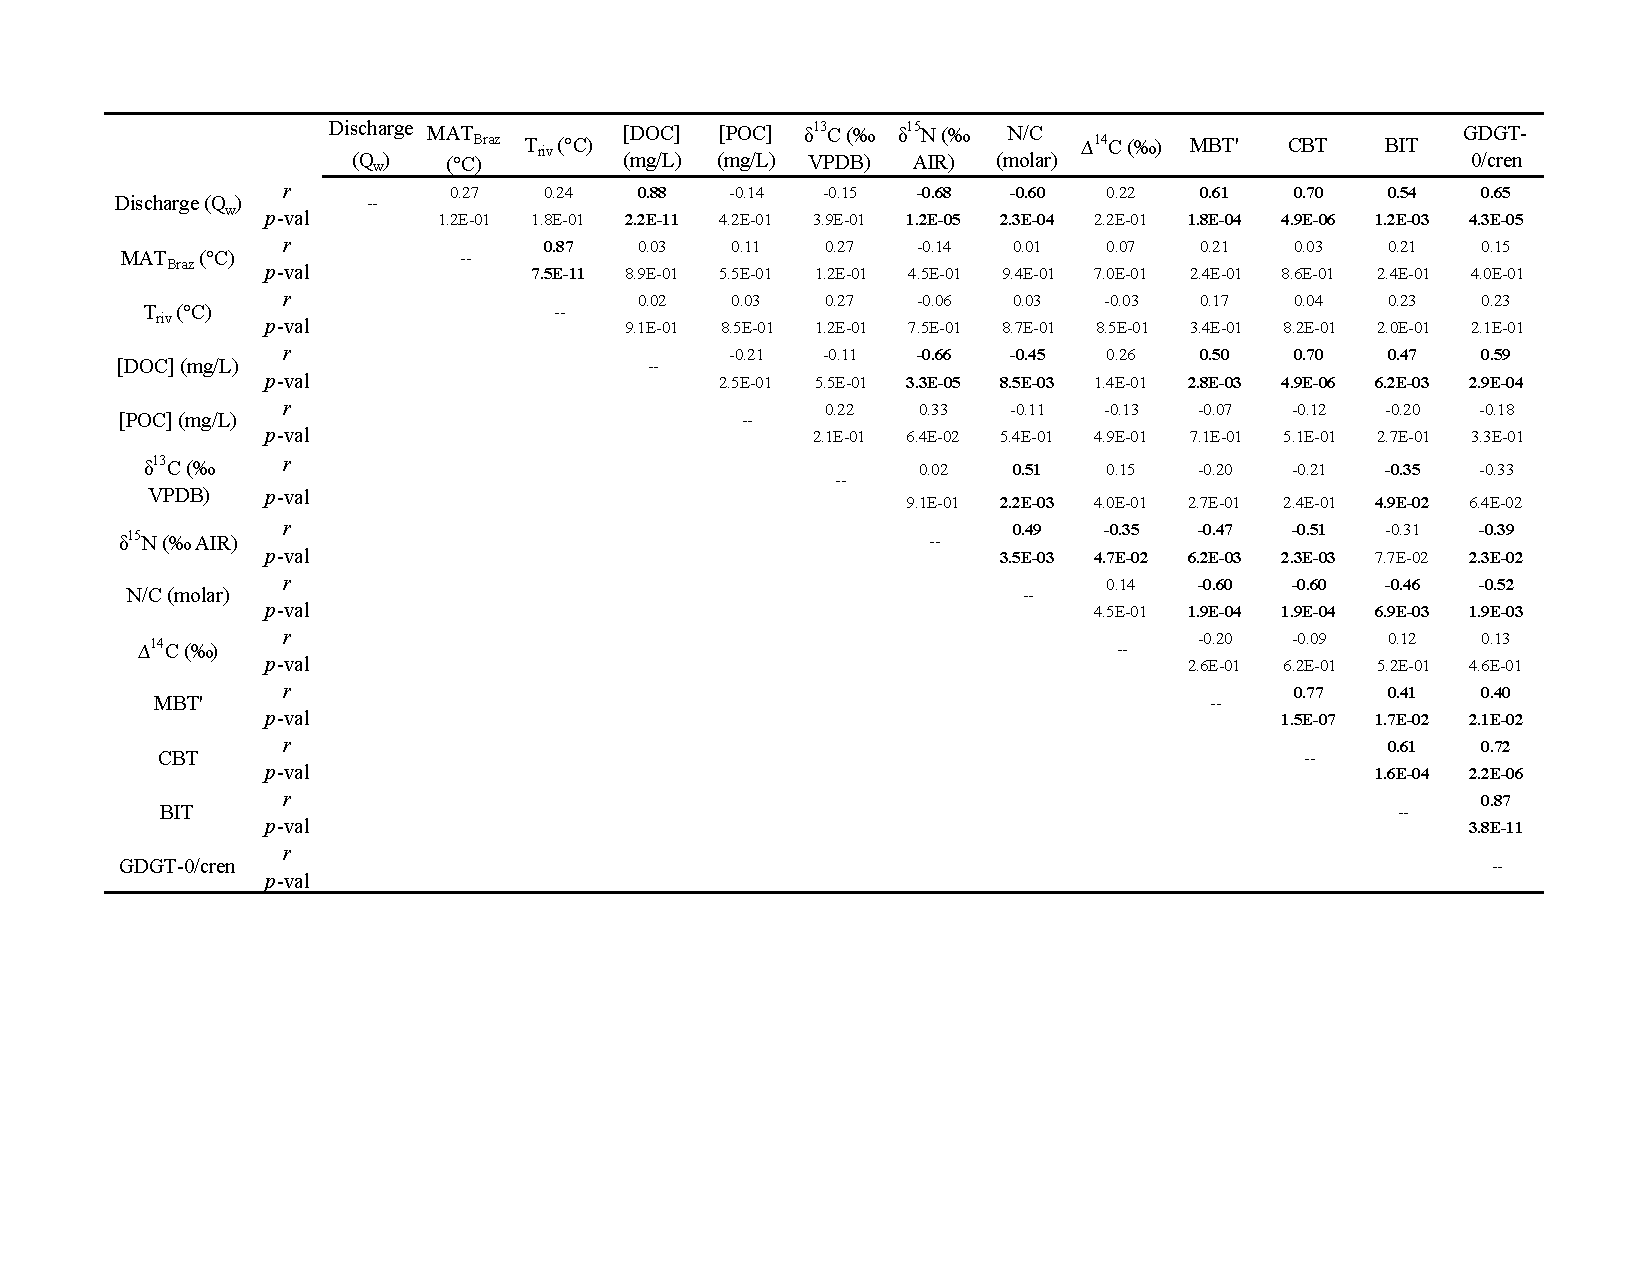
\includegraphics{Thesis_Tables/Ch5Tab2}
	\label{Ch5Tab:2} 
\end{sidewaystable}

\subsection{Bulk measurements}

\subsubsection{DOC and POC concentrations}

Congo River [DOC] ranges from $5.1$ mg L\textsuperscript{-1} in June 2011 to $14.2$ mg L\textsuperscript{-1} in October 2012 (mean = $9.0 \pm 2.5$ mg L\textsuperscript{-1}; Figure \ref{Ch5Fig:2}E) and exhibits significant correlations with Q\textsubscript{w} (positive), \ce{\delta^{15}N} (negative), N/C (negative), and all GDGT metrics (all positive; Table \ref{Ch5Tab:2}). POC concentration ([POC]) ranges from a minimum of $0.6$ mg L\textsuperscript{-1} in August 2013 to a maximum of $2.6$ mg L\textsuperscript{-1} in February 2011 \citep[mean = $1.3 \pm 0.4$ mg L\textsuperscript{-1}; Figure \ref{Ch5Fig:2}F;][]{Hemingway:2016bq} and is uncorrelated with all environmental parameters, bulk measurements, and GDGT metrics (Table \ref{Ch5Tab:2}). For the Djoue River time-series, [POC] ranges from $0.6$ mg L\textsuperscript{-1} in August 2011 to $1.1$ mg L\textsuperscript{-1} in April, June, and November 2011 (mean = $0.9 \pm 0.2$ mg L\textsuperscript{-1}). Unlike the Congo River, Djoue [POC] exhibits a statistically significant positive correlation with bulk \ce{\delta^{13}C} ($r = 0.60$, $p$-value = $3.05 \times 10^{-2}$, $n = 13$; not shown).

\subsubsection{Stable isotope (\ce{^{13}C}, \ce{^{15}N}) and N/C composition}

\ce{\delta^{13}C} values of Congo River POC across the time-series range from $-27.6$\textperthousand\ (November--December 2010) to $-24.6$\textperthousand\ (February 2013), averaging $-26.4 \pm 0.7$\textperthousand\ (Figure \ref{Ch5Fig:3}A). Additionally, \ce{\delta^{13}C} values exhibit a statistically significant positive relationship with N/C and a negative relationship with BIT (Table \ref{Ch5Tab:2}). Djoue River POC \ce{\delta^{13}C} values are statistically identical to those of the Congo River, with a range of $-28.1$\textperthousand\ (August 2011) to $-26.5$\textperthousand\ (April 2011) and a mean of $-27.5 \pm 0.5$\textperthousand.

The nitrogen stable isotope composition of Congo River POM is slightly more variable than that of carbon, with \ce{\delta^{15}N} values ranging from $3.9$\textperthousand\ (December 2012--January 2013) to $8.5$\textperthousand\ (August 2011; mean = $6.1 \pm 1.1$\textperthousand; Figure \ref{Ch5Fig:3}B). \ce{\delta^{15}N} values display a strong negative correlation with both Q\textsubscript{w} and [DOC], as well as weaker correlations with N/C (positive), \ce{\Delta^{14}C} (negative), MBT', CBT, and GDGT-0/cren (all negative; Table \ref{Ch5Tab:2}). As with \ce{\delta^{13}C}, Djoue River \ce{\delta^{15}N} values span a similar range as those of the Congo River ($3.8$\textperthousand\ in December 2010 to $6.4$\textperthousand\ in August 2011), with a mean value of $5.0 \pm 0.7$\textperthousand.

Congo River N/C ranges from $0.076$ (December 2010) to $0.118$ (August 2012) with an average of $0.096 \pm 0.010$ (Figure \ref{Ch5Fig:3}C). Like \ce{\delta^{15}N} values, N/C displays a negative correlation with Q\textsubscript{w} and [DOC], and is additionally negatively correlated with all GDGT metrics and positively correlated with \ce{\delta^{13}C} and \ce{\delta^{15}N} (Table \ref{Ch5Tab:2}). Unlike stable isotopes, the Djoue River time-series average N/C value is statistically lower than that of the Congo River ($p$-value = $1.10 \times 10^{-2}$), with individual samples ranging from a minimum of $0.050$ (January, May 2011) to a maximum of $0.080$ (April 2011; mean = $0.065 \pm 0.010$).

% Figure 3
\begin{figure}[ht]
	\makebox[\textwidth][c]{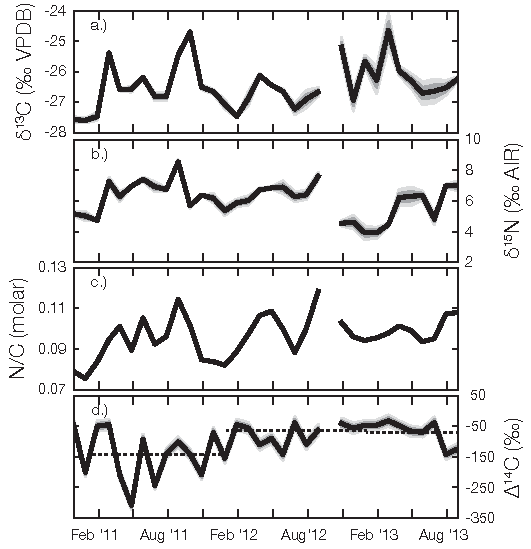
\includegraphics[]{Thesis_Figures/Ch5Fig3}}
	\caption[Bulk parameter time-series plots]{Time-series plots of Congo River bulk POM molecular and isotopic composition: $(A)$ \ce{\delta^{13}C}, $(B)$ \ce{\delta^{15}N}, $(C)$ N/C, and $(D)$ \ce{\Delta^{14}C}. Where visible, dark gray envelope is $\pm 1 \sigma$ uncertainty and light gray envelope is 95\% confidence interval. Dotted lines in panel $(D)$ are the flux-weighted-average values for each calendar year (January--August only for 2013).}
	\label{Ch5Fig:3} 
\end{figure}

\subsubsection{\ce{^{14}C} composition}

Radiocarbon composition of exported Congo River POC is highly variable, with \ce{\Delta^{14}C} ranging from $-309$\textperthousand\ in April 2011 to $-33$\textperthousand\ in February 2013 (mean = $-105 \pm 69$\textperthousand; Figure \ref{Ch5Fig:3}D). Because \ce{\Delta^{14}C} is more depleted and variable during 2011 as opposed to 2012 and 2013, there exists a statistically significant positive temporal trend throughout the time-series, with an increase of $32.5$\textperthousand/year ($r = 0.39$, $p$-value = $2.80 \times 10^{-2}$). Additionally, \ce{\Delta^{14}C} displays a slight negative correlation with \ce{\delta^{15}N} as described above, but is uncorrelated with all other environmental variables, bulk measurements, and GDGT metrics (Table \ref{Ch5Tab:2}).

\subsection{GDGT distributions}

Homologue brIa is the most abundant brGDGT throughout the time-series, contributing between $73$ and $82$\% of total brGDGTs (mean = $77 \pm 2$\%; Table \ref{Ch5Tab:S2}). Homologues brIIa (mean = $14 \pm 1$\%) and brIb (mean = $5 \pm 1$\%) are consistently the second- and third-most abundant branched homologues, respectively. All remaining branched homologues contribute $1-2$\% of the brGDGT total, with the exception of brIIIc which was not detected in any sample. This leads to an MBT' range of $0.80 - 0.86$ (mean = $0.84 \pm 0.01$) and a CBT range of $1.00 - 1.32$ (mean = $1.15 \pm 0.08$; Figure \ref{Ch5Fig:4}A, Figure \ref{Ch5Fig:4}B). IsoGDGTs are significantly less abundant than branched compounds, with total isoGDGTs (crenarchaeol and GDGT-0 only) comprising between $5$ and $10$\% of the brGDGT total (mean = $6 \pm 1$\%). Resulting in BIT values are consistently $\geq 0.96$ (Figure \ref{Ch5Fig:4}C). With the exception of July and August 2013, GDGT-0 is more abundant than crenarchaeol, comprising $60 \pm 6$\% of isoGDGTs, and resulting in a GDGT-0/cren ratio ranging from $0.7$ to $2.4$ (mean = $1.6 \pm 0.4$; Figure \ref{Ch5Fig:4}D). All GDGT metrics are positively correlated with each other and exhibit strong positive correlations with Q\textsubscript{w} and [DOC], as well as negative correlations with \ce{\delta^{15}N} (excluding BIT) and N/C (Table \ref{Ch5Tab:2}).

% Figure 4
\begin{figure}[ht]
	\makebox[\textwidth][c]{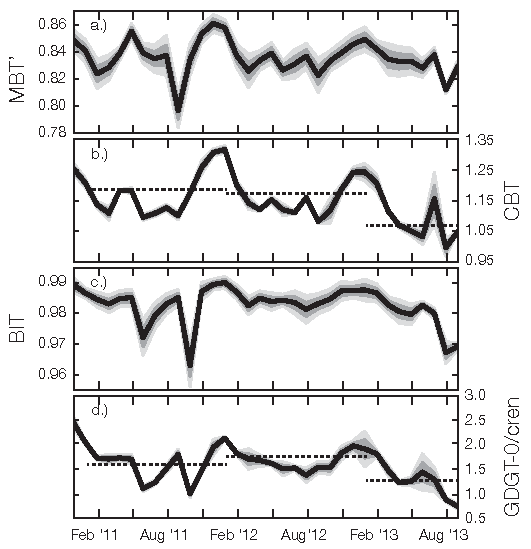
\includegraphics[]{Thesis_Figures/Ch5Fig4}}
	\caption[GDGT metric time-series plots]{Time-series plots of Congo River GDGT distribution metrics: $(A)$ MBT', $(B)$ CBT, $(C)$ BIT, and $(D)$ GDGT-0/cren. Where visible, dark gray envelope is $\pm 1 \sigma$ uncertainty and light gray envelope is 95\% confidence interval. Dotted lines in panels $(B)$ and $(D)$ are the flux-weighted-average values for each calendar year (January--August only for 2013).}
	\label{Ch5Fig:4} 
\end{figure}

\section{Discussion}

\subsection{OC fluxes, yield, and the importance of the \textit{Cuvette Congolaise}}

Congo River [POC] in our dataset is in good agreement with previously published values from nearby sampling sites \citep{Mariotti:1991vx,Coynel:2005cn,Spencer:2012en,Spencer:2016ho}. The time-series average reported here (mean = $1.3 \pm 0.4$ mg L\textsuperscript{-1}) is slightly lower than that of \citet{Mariotti:1991vx} from the years 1976 and 1983 (mean = $2.0 \pm 0.2$ mg L\textsuperscript{-1}, $n = 10$) and of \citet{Coynel:2005cn} from the years 1990--1993 (mean = $1.74$ mg L\textsuperscript{-1}, $n = 23$), but is similar to the recent measurements of \citet{Spencer:2012en,Spencer:2016ho} (mean = $1.5 \pm 0.3$ mg L\textsuperscript{-1}, $n = 19$). While less data exist for the Djoue River, [POC] from our time-series is nearly identical to that of \citet{Mariotti:1991vx} (mean = $0.7 \pm 0.1$ mg L\textsuperscript{-1}, $n = 3$).

Suspended sediment export from the Congo River, both in terms of TSS concentration and yield, is significantly lower than for other large temperate and tropical rivers across the globe \citep{Ludwig:1998ud,Milliman:2011ug,Galy:2015fx}. However, TSS exhibit high \%OC values leading to [POC] near that of other tropical rivers such as the Amazon \citep{Richey:1990wl}. Calculated POC yield using our time-series is $0.42 \pm 0.004$ tC km\textsuperscript{-2} yr\textsuperscript{-1} between November 2010 and August 2013, slightly lower than previously published values of $0.68$ tC km\textsuperscript{-2} yr\textsuperscript{-1} \citep{Ludwig:1996ul} and $0.55$ tC km\textsuperscript{-2} yr\textsuperscript{-1} \citep{Coynel:2005cn,Spencer:2016ho}. Annual POC yield for the entire Congo basin is greater than that of the Oubangui sub-basin ($0.26$ tC km\textsuperscript{-2} yr\textsuperscript{-1}) due to the fact that northern-hemisphere summer base-flow conditions lead to reduced Oubangui River POC fluxes \citep{Bouillon:2012cw}.

While most rivers display clear positive, nonlinear relationships between discharge, TSS yield, and POC yield (\textit{i.e.} rating curves), such trends are significantly weaker in the Congo River due to a lack of correlation between Q\textsubscript{w} and [POC] (Table \ref{Ch5Tab:2}). This result is at least partially due to hysteresis effects. Highest [POC] is generally observed during the rising limb of the hydrograph (Sep-Oct-Nov) due to the flushing of sediments previously entrained in the \textit{Cuvette Congolaise}, while the falling limb (Dec-Jan-Feb) exhibits lower [POC] for similar discharge values \citep{Spencer:2016ho}. Furthermore, during boreal spring and summer when water flux through this region is low and non-erosive \citep{Bricquet:1993ve,Henchiri:2016jh}, the \textit{Cuvette Congolaise} acts as sediment trap, removing POM derived from right-bank and main-stem headwaters \citep{Laraque:2009fz}.

In contrast to POC, Congo River DOC follows typical rating curve behavior due to the strong positive correlation between Q\textsubscript{w} and [DOC] (Table \ref{Ch5Tab:2}), as has been reported previously \citep{Coynel:2005cn,Wang:2013js,Spencer:2016ho}. Still, [DOC] does display a slight hysteresis effect, with highest concentrations observed during the rising limb of the hydrograph (Sep-Oct-Nov). This result is again due to flushing of \textit{Cuvette}-derived DOC at this time, as swamp-forest tributaries within the Congo basin have been shown to reach [DOC] values as high as $\approx 80$ mg L\textsuperscript{-1} \citep{Mann:2014jx}. Resulting DOC yield over the course of our time-series is $3.11 \pm 0.03$ tC km\textsuperscript{-2} yr\textsuperscript{-1}, leading to a dissolved-phase contribution to total exported OC of $87 \pm 5$\%. Annual yield calculated here is within the range of previously reported estimates [$2.47$ tC km\textsuperscript{-2} yr\textsuperscript{-1} \citep{Ludwig:1996ul}, $3.44$ tC km\textsuperscript{-2} yr\textsuperscript{-1} \citep{Coynel:2005cn}, $3.48$ tC km\textsuperscript{-2} yr\textsuperscript{-1} \citep{Spencer:2016ho}], and is roughly double that of the Oubangui sub-basin [$1.43$ tC km\textsuperscript{-2} yr\textsuperscript{-1} \citep{Bouillon:2012cw}].

\subsection{Congo River POM sources: Insight from bulk measurements}

Like concentration and flux results, Congo River POM isotope and N/C composition presented here agrees with previously published values from nearby sampling sites \citep{Mariotti:1991vx,Spencer:2012en,Spencer:2016ho}. While our results represent OM contained in bulk TSS, they are nearly identical to published results from the fine fraction only ($<63 \mu$m), as this contains $>80$\% of total POM \citep{Spencer:2012en}. In contrast, coarse material ($\geq63 \mu$m) has been shown to display significantly lower N/C ratios (Figure \ref{Ch5Fig:5}A) as well as \ce{\Delta^{14}C} values $>0$\textperthousand\ due to incorporation of bomb-derived \ce{^{14}C} (Figure \ref{Ch5Fig:5}B), and has been interpreted as representing recently fixed rainforest vegetation and plant debris \citep{Spencer:2012en}. 

% Figure 5
\begin{figure}[p]
	\makebox[\textwidth][c]{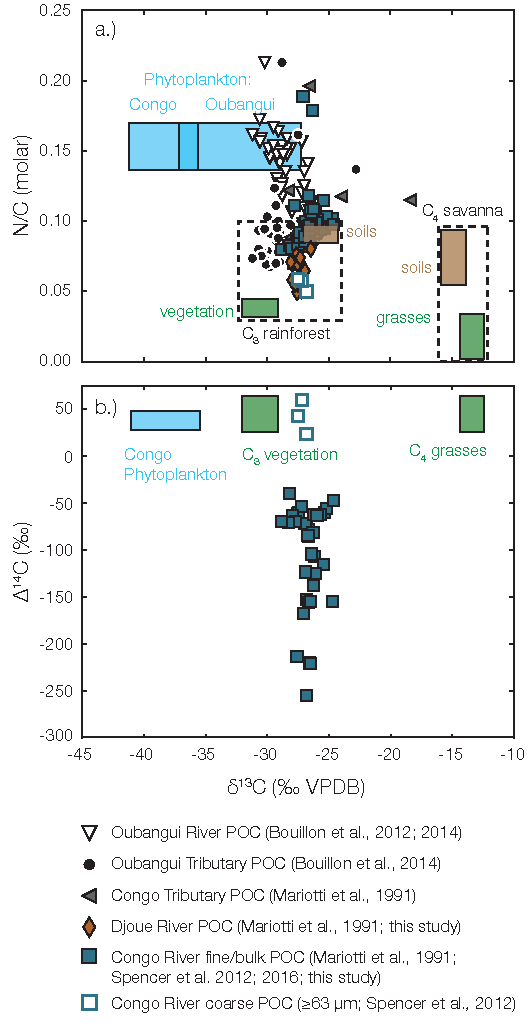
\includegraphics[]{Thesis_Figures/Ch5Fig5}}
	\caption[Conservative tracer mixing model]{Conservative tracer mixing model plots showing all published POM data from within the Congo basin: $(A)$ \ce{\delta^{13}C} vs. N/C and $(B)$ \ce{\delta^{13}C} vs. \ce{\Delta^{14}C}. End-member compositions are listed in Table \ref{Ch5Tab:3} and described in section \ref{Ch5SD2}.}
	\label{Ch5Fig:5} 
\end{figure}

Generally, Congo River main-stem POM is more enriched in \ce{^{13}C} and depleted in N/C relative to the Oubangui River during similar discharge regimes \citep[Figure \ref{Ch5Fig:6}A--B;][]{Bouillon:2012cw,Bouillon:2014ko} and plots within the C\textsubscript{3} rainforest end-member range (Table \ref{Ch5Tab:3}; Figure \ref{Ch5Fig:5}A; see Supplemental Discussion \ref{Ch5SD2} on end-member compositions), indicating that headwater material is diluted and/or replaced during transit through the \textit{Cuvette Congolaise}. Furthermore, predominantly C\textsubscript{4}-savanna-derived POM is never observed (Figure \ref{Ch5Fig:5}A) despite large regions of C\textsubscript{4} landcover, especially in southern-hemisphere tributary and Djoue River catchments (Table \ref{Ch5Tab:1}; Figure \ref{Ch5Fig:1}B). This agrees with the \ce{^{13}C} composition of plant-wax \textit{n}-alcohols and \textit{n}-alkanoic acids \citep{Hemingway:2016bq} and the molecular composition of lignin phenols \citep{Spencer:2016ho} extracted from Congo River TSS, which preclude large C\textsubscript{4}-grass inputs to these biomarker classes. However, left-bank tributaries such as the Kasai River exhibit the highest TSS yield within the Congo basin \citep{Laraque:2009fz}, suggesting that a non-negligible fraction of exported POM is derived from this region, except during 2011 when southern-hemisphere discharge was anomalously low (Figure \ref{Ch5Fig:2}A). The lack of significant C\textsubscript{4} contribution observed throughout our Congo River and Djoue River time-series likely supports the idea that exported bulk POM signals bias toward riparian zones \citep{Bouillon:2012cw}, as these regions are dominated by C\textsubscript{3} landcover throughout the basin (Figure \ref{Ch5Fig:1}). However, we note that, in contrast to all other signals, \ce{^{13}C}-enriched C\textsubscript{33} and C\textsubscript{35} \textit{n}-alkanes have been observed in the Congo River, indicating the persistence of distal C\textsubscript{4} inputs to these low concentration, recalcitrant biomarkers \citep{Hemingway:2016bq}.

% Table 3
\begin{sidewaystable}[p]
	\caption[Mixing model end-member compositions]{Mixing model end-member compositions. See section \ref{Ch5SD2} for further discussion.}
	\centering
		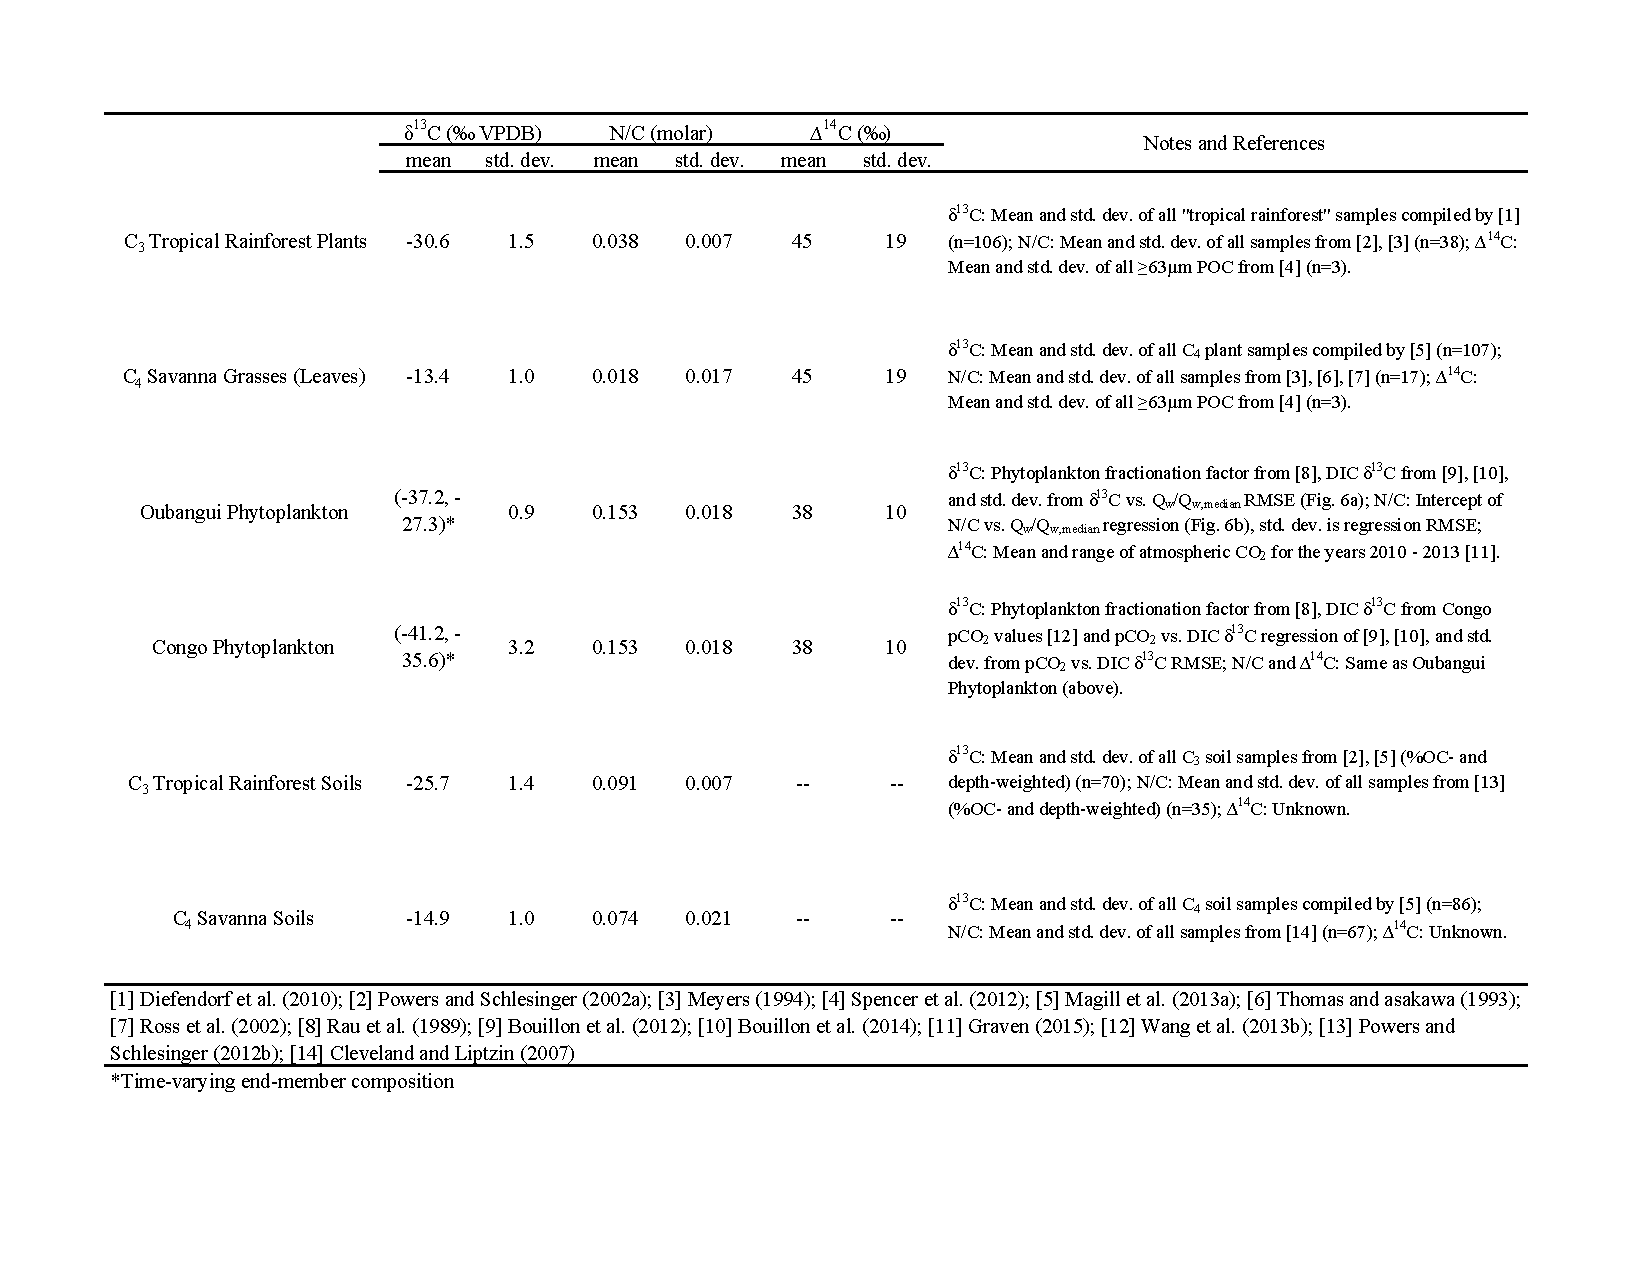
\includegraphics{Thesis_Tables/Ch5Tab3}
	\label{Ch5Tab:3} 
\end{sidewaystable}

Additionally, significant OC\textsubscript{petro} erosion in the Congo basin is unlikely due to the low catchment relief and lack of OC-rich bedrock lithology \citep{Copard:2007bf,Milliman:2011ug}. We therefore omit C\textsubscript{4}-savanna and OC\textsubscript{petro} sources form our mixing model and quantitatively calculate the contributions of C\textsubscript{3} tropical rainforest vegetation, C\textsubscript{3} tropical rainforest soils, and autochthonous phytoplankton to Congo River \citep[][this study]{Spencer:2016ho} and Oubangui River POM \citep{Bouillon:2012cw,Bouillon:2014ko}. We retain \ce{\delta^{13}C} and N/C as conservative tracers, as \ce{\Delta^{14}C} of eroded soils is highly variable and difficult to constrain \textit{a priori}, while absolute \ce{\delta^{15}N} values of vegetation, soils, and phytoplankton are influenced by unknown nitrogen sources, fixation pathways, and (re)cycling \citep{Martinelli:1999ta,Kendall:2001bs}. Resulting end-member contributions are reported in Table \ref{Ch5Tab:S3}. 

% Figure 6
\begin{figure}[p]
	\makebox[\textwidth][c]{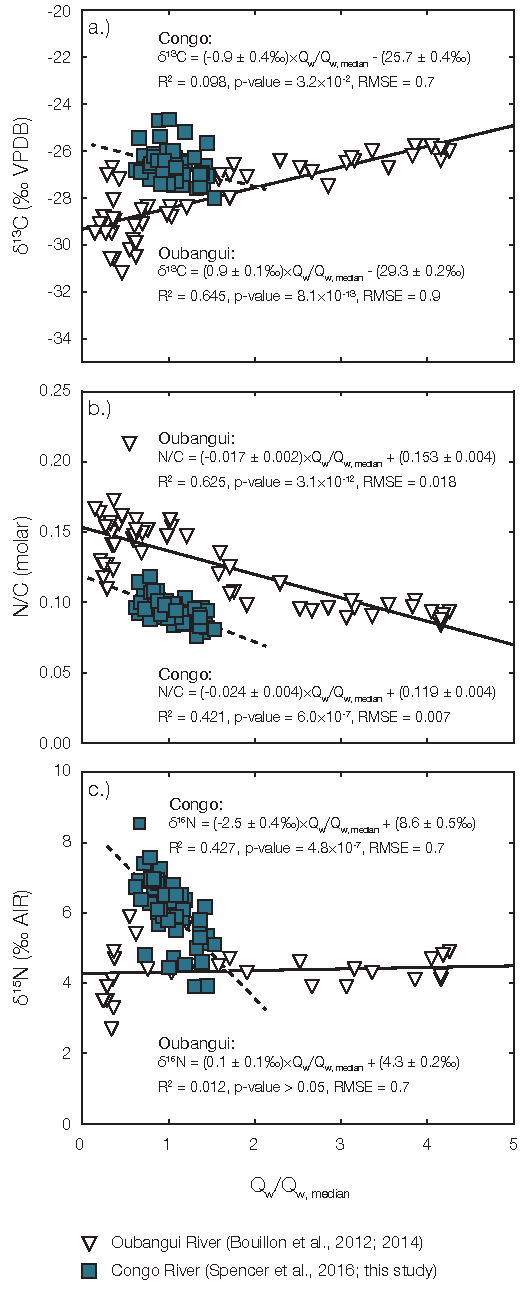
\includegraphics[scale=0.9]{Thesis_Figures/Ch5Fig6}}
	\caption[Discharge vs. \ce{\delta^{13}C}, N/C, and \ce{\delta^{15}N}]{Correlations between Congo River and Oubangui River discharge vs. $(A)$ \ce{\delta^{13}C}, $(B)$ N/C, and $(C)$ \ce{\delta^{15}N}. To present both records on the same scale, discharge has been normalized by the median discharge value for each time-series (Q\textsubscript{w}/Q\textsubscript{w, median}).}
	\label{Ch5Fig:6} 
\end{figure}

\subsubsection{Seasonal source variability}

Congo River POM at Brazzaville/Kinshasa is consistently dominated by C\textsubscript{3} soil material (median = $87$\%, inter-quartile range = $80 - 91$\%; Figure \ref{Ch5Fig:7}A), with low contribution by C\textsubscript{3} tree litter (median = $1$\%, inter-quartile range = $0 - 13$\%; Figure \ref{Ch5Fig:7}B) and autochthonous phytoplankton production (median = $8$\%, inter-quartile range = $6 - 11$\%; Figure \ref{Ch5Fig:7}C). In contrast, Oubangui River POM is composed almost entirely of C\textsubscript{3} rainforest soils when discharge is high (median = $33$\%, inter-quartile range = $8 - 86$\%; Figure \ref{Ch5Fig:7}A) and phytoplankton sources during base-flow conditions (median = $62$\%, inter-quartile range = $11 - 92$\%; Figure \ref{Ch5Fig:7}C), with minimal contribution by C\textsubscript{3} rainforest vegetation throughout the hydrograph (median = $0$\%, inter-quartile range = $0 - 2$\%; Figure \ref{Ch5Fig:7}B). 

Seasonal importance of phytoplankton-derived POM in the Oubangui River therefore does not propagate to the main-stem Congo River at Brazzaville/Kinshasa (Figure \ref{Ch5Fig:7}C) due to a combination of: $(i)$ dilution by downstream inputs, $(ii)$ remineralization during transit, and/or $(iii)$ loss due to particle settling/trapping within the \textit{Cuvette Congolaise} when water flux through this region is low \citep{Laraque:2009fz}. However, while low throughout the time-series, phytoplankton contribution to Congo River POM does display a statistically significant decrease with increasing discharge ($r = -0.60$, $p$-value = $6.10 \times 10^{-6}$, $n = 48$; Figure \ref{Ch5Fig:7}C). This result agrees with observed seasonal trends in C\textsubscript{24} \textit{n}-alcohol \ce{^{13}C} composition, as this compound has been shown to be influenced by autochthonous production \citep{Hemingway:2016bq}.

Unlike phytoplankton, C\textsubscript{3} vegetation contribution to POC is typically higher in the Congo River main-stem than in the Oubangui River and is positively correlated with discharge ($r = 0.57$, $p$-value = $1.98 \times 10^{-5}$, $n = 48$; Figure \ref{Ch5Fig:7}B), reflecting increasing admixture of less degraded vascular plant material when water flux through the \textit{Cuvette Congolaise} is high. While absolute end-member \ce{\delta^{15}N} values are difficult to constrain \textit{a priori}, a compilation of tropical rainforest samples indicates that fresh vegetation is depleted in \ce{^{15}N} by $6.9 \pm 4.5$\textperthousand\ relative to soils \citep{Martinelli:1999ta}. In contrast, \ce{\delta^{15}N} of Oubangui River POM is constant across the hydrograph (Figure \ref{Ch5Fig:6}C) and suggests that this tracer is insensitive to phytoplankton vs. C\textsubscript{3}-soil inputs in this system, although we note that Congo River POM end-member compositions are likely not identical to those in the Oubangui. Still, the strong negative correlation between Congo River POM \ce{\delta^{15}N} and discharge observed here (Figure \ref{Ch5Fig:6}C) is further evidence for an increase in fresh vascular plant material with increasing discharge. This result is additionally supported by observed seasonal variability in the chemical composition and carbon-normalized yield of particulate lignin phenols, which shift toward higher yield and less degraded signatures when discharge is high \citep{Spencer:2016ho}.

% Figure 7
\begin{figure}[p]
	\makebox[\textwidth][c]{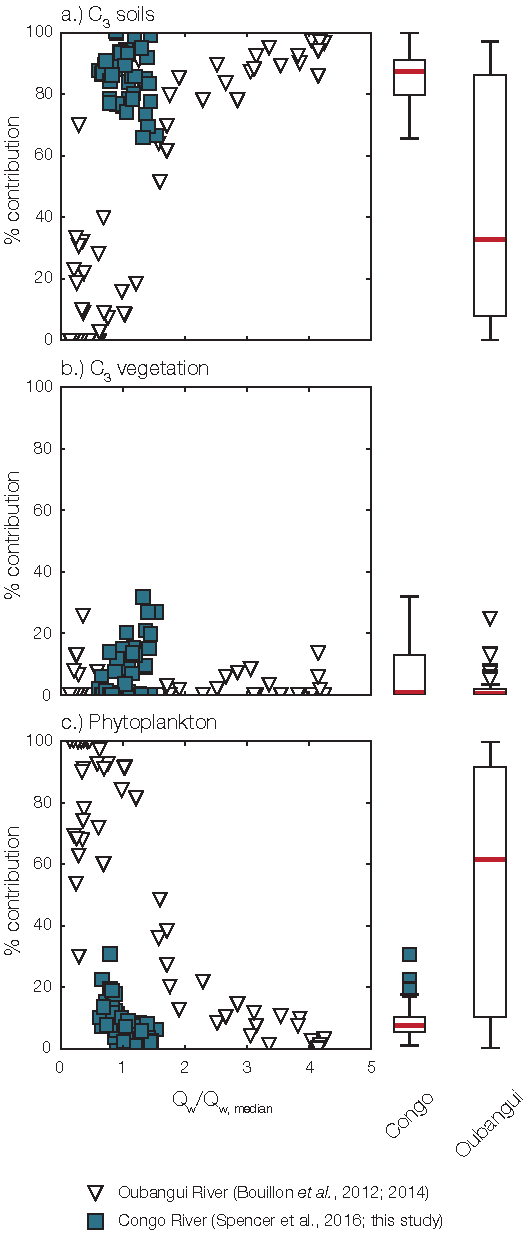
\includegraphics[scale=0.9]{Thesis_Figures/Ch5Fig7}}
	\caption[Discharge vs. end-member fractional contribution]{Fractional contribution box plots and correlations with discharge for: $(A)$ C\textsubscript{3} soils, $(B)$ C\textsubscript{3} vegetation, and $(C)$ phytoplankton. To present both records on the same scale, discharge has been normalized by the median discharge value for each time-series (Q\textsubscript{w}/Q\textsubscript{w, median}). For box plots, red lines are median values, boxes contain the inter-quartile range, and whiskers contain the 95\% confidence interval. Individual outliers are plotted as blue squares (Congo) and white triangles (Oubangui).}
	\label{Ch5Fig:7} 
\end{figure}

\subsubsection{Controls on soil \ce{\Delta^{14}C}}

While consistently dominated by C\textsubscript{3}-soil material, the \ce{^{14}C} composition of exported Congo River POC is highly variable, especially in 2011 when southern-hemisphere discharge was lowest (Figure \ref{Ch5Fig:3}D). Observed \ce{\Delta^{14}C} values cannot be explained by OC\textsubscript{petro} inputs due to low erosion rates and a lack of OC-rich bedrock in the Congo basin \citep{Copard:2007bf}, and are therefore interpreted to reflect variable ages of eroded soils. We calculate the \ce{^{14}C} composition of exported soil-derived POC using the equation:

% Equation 4
\begin{equation}\label{Ch5Eq:4}
	\ce{\Delta^{14}C}_{\text{soil}} = \frac{1}{f_{\text{soil}}} \left(\ce{\Delta^{14}C}_{\text{POC}} - f_{\text{phyto}}\ce{\Delta^{14}C}_{\text{phyto}} - f_{\text{plants}}\ce{\Delta^{14}C}_{\text{plants}} \right)
\end{equation}

where $f_i$ is the calculated fractional contribution of end member $i$ (Table \ref{Ch5Tab:S3}), \ce{\Delta^{14}C}\textsubscript{POC} is the measured POC \ce{\Delta^{14}C} value (Table \ref{Ch5Tab:S1}), and \ce{\Delta^{14}C}\textsubscript{phyto} and \ce{\Delta^{14}C}\textsubscript{plants} are phytoplankton and C\textsubscript{3} tropical rainforest vegetation end-member values (Table \ref{Ch5Tab:3}; Figure \ref{Ch5Fig:5}B). 

Eroded soil-derived POC exhibits low and variable \ce{\Delta^{14}C} values during 2011 (annual mean = $-176 \pm 93$\textperthousand) as compared to 2012 (annual mean = $-90 \pm 39$\textperthousand) and 2013 (Jan--Aug mean = $-85 \pm 53$\textperthousand), suggesting that anomalously low southern-hemisphere discharge in 2011 resulted in a bias toward export of pre-aged, \textit{Cuvette}-derived soils at this time. In contrast, \ce{\Delta^{14}C} values of soil-derived POC were near $-50$\textperthousand\ from January to June 2013, when left-bank tributary discharge peaked above the 1977--2006 average for these months (Figure \ref{Ch5Fig:2}A). Ecosystems drained by left-bank tributaries in the Congo basin (grassland, woodland/shrubland, Figure \ref{Ch5Fig:1}A) are highly productive with most biomass being produced as leaves and foliage \citep{Bloom:2016gm}, resulting in a large carbon input flux to soils and thus short soil residence times \citep{Carvalhais:2014dc}. Combined with relatively high TSS yields in these tributaries \citep{Laraque:2009fz}, this supports our interpretation that increased precipitation and discharge in the southern half of the basin leads to higher \ce{^{14}C} content of exported soil-derived POC.

Furthermore, increased terrestrial reservoir ages (\textit{i.e.} lower \ce{^{14}C} composition relative to the atmosphere at the time of deposition) since the Early- to Mid-Holocene have been observed in plant-wax lipids, wood pieces, and OC extracted from Congo Fan sediments, concomitant with decreasing precipitation intensity at this time \citep{Schefuss:2005jo}, and have been interpreted as reflecting erosion of pre-aged, previously inundated \textit{Cuvette Congolaise} swamp deposits \citep{Schefuss:2016cp}. These results indicate that \textit{Cuvette}-derived POM contains eroded soils with lower \ce{^{14}C} content than those sourced from other ecosystems within the basin, likely due to efficient OC preservation under permanently inundated, anoxic conditions. The time-series \ce{\Delta^{14}C} results presented here further support this idea, and show that relative changes in \textit{Cuvette Congolaise} inputs leads to variability in exported POC ages on inter-annual timescales in addition to the millennial-timescale variability described in \citet{Schefuss:2016cp}. Thus, if the observed decreases in Apr-May-Jun precipitation in the Congo basin over the past decade continue \citep{Zhou:2014gl}, our data suggest that exported soil-derived POM will further bias toward protracted \textit{Cuvette Congolaise} sources under future discharge regimes. Because OM stored under anoxic conditions has been shown to be highly susceptible to degradation upon exposure to O2 \citep{Hoefs:2002wu}, increasing relative contribution by this end-member to exported POM could additionally result in increased remineralization during fluvial transit.

\subsection{Congo River POM sources: Insight from GDGT metrics}

Congo River GDGTs can provide further information regarding POM provenance, especially since variability in material sourced from the highly acidic, anoxic \textit{Cuvette Congolaise} \citep{Mann:2014jx} should be reflected in CBT and GDGT-0/cren metrics \citep{Blaga:2009ge,Peterse:2012bs}. Indeed, these indices display large variability throughout the time-series (Figure \ref{Ch5Fig:4}B, D), indicating significant seasonal changes in GDGT source. Although GDGT distributions for each end member could not be measured directly, redundancy analysis \citep[RDA;][]{Legendre:1998tt} indicates that a majority of variance in GDGT metrics can be described by a canonical axis that is strongly correlated with hydrology (Table \ref{Ch5Tab:S4}; Figure \ref{Ch5Fig:8}). Analagous to bulk POM results, this suggests a hydrologic control on GDGT sources and molecular distributions in Congo River TSS. 

It is possible that seasonal variability is due to \textit{in situ} brGDGT production within the river when discharge is low, as this would lead to the observed decreases in MBT' and CBT at this time \citep{Peterse:2009hl,Tierney:2010br} and has previously been invoked to explain brGDGT distributions in other river systems \citep{DeJonge:2014fs,Zell:2014gt}. However, significant \textit{in situ} brGDGT production within the water column on seasonal timescales is unlikely, as these compounds have been shown to exhibit much longer growth times. For example, \citet{Peterse:2015ef} observed no \textit{in situ} production of intact polar brGDGTs in 160-day incubations of TSS from New Zealand rivers. While the incubation conditions of \citet{Peterse:2015ef} are not identical to those within the Congo River, significant autochthonous production would additionally lead to bulk N/C enrichment and \ce{^{13}C} depletion during low discharge, which is clearly not observed (Figure \ref{Ch5Fig:3}A, \ref{Ch5Fig:3}C).

% Figure 8
\begin{figure}[ht ]
	\makebox[\textwidth][c]{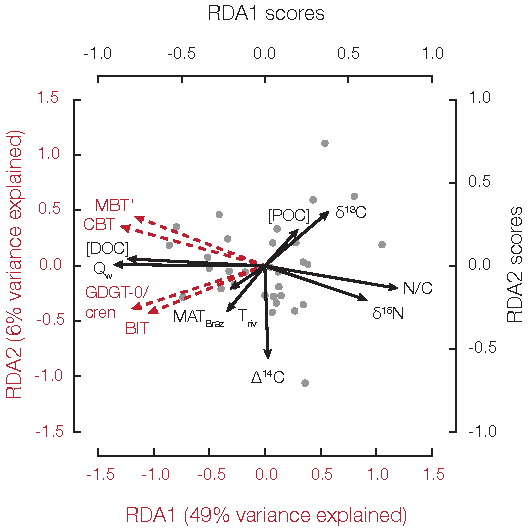
\includegraphics[]{Thesis_Figures/Ch5Fig8}}
	\caption[Environmental parameter, bulk metrics, and GDGT distribution RDA analysis]{Congo River time-series RDA triplot ("Type III" scaling) showing the first (RDA1) and second (RDA2) canonical axes. Environmental variable scores are plotted as black arrows, response variable ("species") scores are plotted as red dashed arrows, and individual sample ("site") scores are plotted as gray circles. Red axes labels correspond to response variable scores while black axes labels correspond to environmental variable scores.}
	\label{Ch5Fig:8} 
\end{figure}

Rather, variability is likely due to incorporation of GDGTs produced in permanently inundated, anoxic \textit{Cuvette Congolaise} soils when discharge through this region is high. This is supported by the observation that water-logged, acidic soils in western Uganda exhibit significantly higher CBT values than well-drained, aerobic soils from the same transect \citep{Loomis:2011dr}. Similarly, water-saturated and oxygen-depleted peat bogs have been shown to display higher CBT values than nearby aerobic sites \citep{Huguet:2010di}, as dissolved oxygen content has been shown to exert a strong control on bacterial community composition \citep{Hansel:2008hp} and likely brGDGT distributions. In our time-series, flux-weighted-average CBT during 2013 is significantly lower than in 2011 and 2012 (Figure \ref{Ch5Fig:4}B), consistent with elevated southern-hemisphere discharge and increased contribution by left-bank POM in 2013.

Additionally, GDGT-0/cren ratios $>2$ are generally thought to represent substantial contribution by anaerobic methanogenic archaea \citep{Blaga:2009ge}. Significant methanogenesis in \textit{Cuvette Congolaise} soils is indirectly supported by the high concentrations and \ce{^{13}C} composition of amino-bacteriohopanepolyls in this region \citep{Talbot:2014jd,SpencerJones:2015bn}. Therefore, in addition to higher CBT values, increased incorporation of GDGTs from swamp-forest soils during high discharge should lead to elevated GDGT-0/cren ratios, as is observed (Figure \ref{Ch5Fig:4}D). Similar to CBT, flux-weighted-average GDGT-0/cren is lowest in 2013 as compared to 2011 and 2012, further supporting the idea that increased left-bank contribution is the source of exported POM with higher \ce{^{14}C} content and less acidic/methanogenic GDGT sources at this time. In contrast, low southern-hemisphere discharge in 2011, and to a lesser degree in 2012 (Figure \ref{Ch5Fig:2}A), leads to exported POM that is biased toward pre-aged \textit{Cuvette Congolaise} soils. Thus, GDGT metrics agree with bulk end-member mixing-model and \ce{\Delta^{14}C} results in highlighting the importance of the \textit{Cuvette Congolaise} in determining exported POM signals from the Congo River.

\section{Conclusion}

We present a 34-month record of Congo River DOC concentrations, POM composition (\ce{\delta^{13}C}, \ce{\delta^{15}N}, \ce{\Delta^{14}C}, N/C), and GDGT distributions to constrain seasonal and inter-annual variability in the source of exported OM. Our results indicate that all Congo River POM samples are consistently dominated by C\textsubscript{3} soil inputs throughout the time-series, with decreasing contribution by phytoplankton and increasing contribution by fresh C\textsubscript{3} vegetation during high discharge. In contrast, large inputs by C\textsubscript{4} grasses are never observed.

Exported soil-derived POC displays low and variable \ce{^{14}C} content, especially during 2011 when southern-hemisphere discharge was anomalously low. Combined with higher CBT and GDGT-0/cren values in 2011, this suggests that acidic, anoxic \textit{Cuvette Congolaise} soils are an important source of pre-aged OM to the Congo River. Furthermore, high southern-hemisphere discharge in spring 2013 coincides with stable, high \ce{^{14}C} content and suggests that left-bank tributaries are a source of young soil-derived POM, consistent with lower CBT and GDGT-0/cren at this time.

This study demonstrates that POM exported from tropical, wet river catchments can contain significantly pre-aged biospheric material due to protracted storage in anoxic soils. We emphasize that permanently inundated areas such as those present in the \textit{Cuvette Congolaise} are an important OM reservoir despite their relatively small landcover extent and could be more significant in determining the role of tropical rivers in the global carbon cycle than previously thought, especially if future hydrologic regimes favor export and remineralization of this material.

%\section*{Acknowledgements}
%We thank Carl Johnson (WHOI), Ekaterina Bulygina (Woods Hole Research Center), Sarah Rosengard (WHOI), Helena Pryer (WHOI), Negar Haghipour (ETH), and Lukas Wacker (ETH) for laboratory assistance. V.V.G. was partly supported by the US National Science Foundation, grants OCE-0851015 and OCE-0928582; J.D.H. was supported by the NSF Graduate Research Fellowship Program under grant number 2012126152; T.I.E. was partly supported by the Swiss National Science Foundation (SNF Grant No. 200021 140850); E.S. was supported by the DFG Research Center/Cluster of Excellence "The Ocean in the Earth System" at MARUM--Center for Environmental Sciences; R.G.M.S. was partly supported by the US National Science Foundation, grants ETBC-0851101, OCE-1333157, and OCE-1464396.

\clearpage

\section{Supplementary Material}

\subsection{Discussion}

\subsubsection{Effect of 6-methyl brGDGTs}\label{Ch5SD1}

Updated chromatographic methods not employed here now allow for the separation of previously co-eluting 5-methyl and 6-methyl brGDGTs and have led to improved metrics for tracking environmental parameters when calibrated using a global soil dataset \citep{DeJonge:2013cr,DeJonge:2014kw,Hopmans:2016fo}. However, the tetramethylated brGDGTs (brIa--brIc), which contribute $\geq 80$\% of total brGDGTs in all samples presented here (Table \ref{Ch5Tab:S2}), exist only as 5-methyl homologues \citep{DeJonge:2013cr}. As such, fractional abundance of 6-methyl compounds only becomes significant at soil pH values greater than $\approx 6$ \citep{DeJonge:2014kw}, suggesting that these homologues are of minimal importance in the highly acidic soils of the Congo basin. 

Indeed, linear regressions of MBT'/CBT and the newly defined MBT'\textsubscript{5ME}/CBT\textsubscript{5ME}, which omit 6-methyl compounds, in tropical acidic soils analyzed by \citet{DeJonge:2014kw} are both statistically identical to the 1:1 line (MBT' vs. MBT'\textsubscript{5ME}: $r = 0.93$, $p$-value = $1.14 \times 10^{-8}$, $n = 19$; CBT vs. CBT\textsubscript{5ME}: $r = 1.00$, $p$-value = $0.0$, $n = 16$; not shown). Additionally, for the samples presented in this study, omission of brIIa and brIIb in Equation \ref{Ch5Eq:3} does not introduce any scatter when compared to calculated CBT ($r = 1.00$, $p$-value = $0.00$, root mean square error = $0.008$), indicating that the trends observed here are robust and are not significantly affected by co-eluting 5-methyl and 6-methyl homologues.

\subsubsection{End-member compositions}\label{Ch5SD2}

Vegetation and soil \ce{\delta^{13}C} and N/C compositions are estimated using all literature values from tropical rainforest and savanna locations, as data from central Africa are sparse or nonexistent, and are presented in Table \ref{Ch5Tab:3} \citep{Thomas:1993us,Meyers:1994wca,Powers:2002ug,Powers:2002wg,Ross:2002vp,Cleveland:2007hka,Diefendorf:2010kb,Magill:2013ab}. We note that aquatic macrophytes are a potentially important source of POM, especially when water flux through the \textit{Cuvette Congolaise} is high. However, \citet{Duarte:1992tp} calculates a macrophyte N/C composition of $0.054 \pm 0.019$, statistically identical to the C\textsubscript{3} tropical rainforest vegetation end-member value used here ($p$-value = $2.10 \times 10^{-1}$), while \citet{Hemingway:2016bq} show that \ce{\delta^{13}C} values of plant waxes extracted from Congo River TSS are insensitive to seasonal variability in macrophyte contribution. Our mixing model therefore cannot resolve terrestrial vs. aquatic C\textsubscript{3} tropical rainforest vegetation and combines these within a single end member.

In contrast to terrestrial inputs, autochthonous phytoplankton biomass is nitrogen-rich, with a canonical N/C value near $0.15$ \citep{Anderson:1994vb}. Additionally, phytoplankton utilize DIC as a carbon source with a fractionation factor ($\Delta\delta^{13}$C = \ce{\delta^{13}C}\textsubscript{product} -- \ce{\delta^{13}C}\textsubscript{source}) near $-21$\textperthousand\ \citep{Rau:1989wr}, leading to highly variable \ce{\delta^{13}C} values due to seasonality in DIC isotope composition \citep{Bouillon:2014ko}. We confirm that phytoplankton in the Congo basin exhibit canonical N/C and $\Delta\delta^{13}$C values by plotting Oubangui discharge vs. POC \ce{\delta^{13}C} (Figure \ref{Ch5Fig:6}A) and N/C (Figure \ref{Ch5Fig:6}A). As discharge approaches zero (\textit{i.e.} when incorporation of allochthonous material would become negligible), regressions point to a phytoplankton end member with \ce{\delta^{13}C} = $-29.3 \pm 0.2$\textperthousand\ and N/C = $0.153 \pm 0.004$, while measured DIC \ce{\delta^{13}C} values are near $-8$\textperthousand\ during base-flow conditions \citep{Bouillon:2012cw}. For the Oubangui River, we therefore calculate phytoplankton \ce{\delta^{13}C} for each sample as the corresponding DIC \ce{\delta^{13}C} value minus $21$\textperthousand\ (Table \ref{Ch5Tab:3}). For the Congo River, DIC \ce{\delta^{13}C} must be estimated using the observed dependence on $p$\ce{CO2} \citep{Bouillon:2014ko} and measured $p$\ce{CO2} values from \citet{Wang:2013js}. We note that the time-series of \citet{Wang:2013js} does not cover the years 2012--2013, and we thus repeat 2011 monthly $p$\ce{CO2} values for these years (Table \ref{Ch5Tab:3}).

Soil \ce{\Delta^{14}C} values cannot be constrained \textit{a priori}, preventing the use of radiocarbon content as a conservative tracer within our mixing model. Because we are unaware of any published \ce{\Delta^{14}C} values for Congo River DIC, we calculate phytoplankton \ce{\Delta^{14}C} as the average value of atmospheric \ce{CO2} between the years 2010 and 2013 \citep{Graven:2015he}. This implicitly assumes a negligible hard-water effect on DIC \ce{\Delta^{14}C}, a reasonable assumption given the extremely low carbonate rock weathering rates \citep[$0.017$ tC km\textsuperscript{-2} yr\textsuperscript{-1};][]{Copard:2007bf}, rapid rates of OM remineralization, and large influence of organic acids in determining DIC speciation and concentration in the Congo River \citep{Wang:2013js}. Additionally, we estimate the \ce{\Delta^{14}C} values of rainforest and savanna vegetation as the average of coarse ($\geq 63 \mu$m) POC reported in \citet{Spencer:2012en}, as this has been shown to contain predominantly vascular plant material and thus tracks the inclusion of bomb-derived \ce{^{14}C} into this end member (Table \ref{Ch5Tab:3}).

\clearpage

\subsection{Supplementary Tables}

% Reset table counter
\renewcommand\thetable{\thechapter.S\arabic{table}}    
\setcounter{table}{0}  

% Change caption justification
\captionsetup[table]{justification=raggedright,singlelinecheck=off}

All supplementary tables for this chapter are available on my personal GitHub website at the following link: \url{https://github.com/FluvialSeds/thesis_master}

% Table S1
\begin{table}[h!]
	\caption[Congo and Djoue River environmental and POM measurements]{Congo and Djoue River environmental parameters (Q\textsubscript{w}, MAT\textsubscript{Braz}, T\textsubscript{riv}, pH\textsubscript{riv}, [DOC], [POC]) and POM composition (\%OC, \%N\textsubscript{org}, \ce{\delta^{13}C}, \ce{\delta^{15}N}, N/C, \ce{\Delta^{14}C}).}
	\label{Ch5Tab:S1} 
\end{table}

% Table S2
\begin{table}[h!]
	\caption[Congo River GDGT fractional abundances and metrics]{Congo River GDGT fractional abundances and distribution metrics (MBT', CBT, BIT, GDGT-0/cren.}
	\label{Ch5Tab:S2} 
\end{table}

% Table S3
\begin{table}[h!]
	\caption[End-member fractional contributions]{Calculated Congo River and Oubangui River POM time-series end-member fractional contributions.}
	\label{Ch5Tab:S3} 
\end{table}

% Table S4
\begin{table}[h!]
	\caption[RDA summary statistics and scores]{Congo River time-series RDA summary statistics, biplot scores, sample ("site") scores, and response variable ("species") scores.}
	\label{Ch5Tab:S4} 
\end{table}

% Reset for future chapters
\renewcommand\thetable{\thechapter.\arabic{table}}

% Reset caption justification
\captionsetup[table]{justification=justified}

\clearpage

\subsection{Supplementary Figures}
% Reset figure counter
\renewcommand\thefigure{\thechapter.S\arabic{figure}}    
\setcounter{figure}{0}  

% Supplementary figures

\begin{figure}[h!]
	\makebox[\textwidth][c]{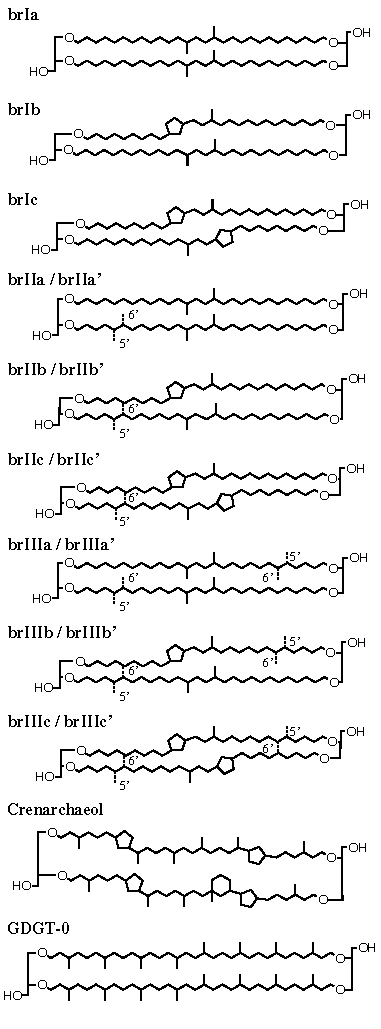
\includegraphics[]{Thesis_Figures/Ch5FigS1}}
	\caption[Core lipid GDGT structures]{Core lipid GDGT structures showing both 5-methyl and 6-methyl homologues for branched compounds.}
	\label{Ch5Fig:S1} 
\end{figure}

% Reset figure style for subsequent chapters
\renewcommand\thefigure{\thechapter.\arabic{figure}}

% Chapter 6 text
\chapter{Rapid microbial oxidation of rock-derived organic carbon in mountain soils}
\label{Ch6}
\raggedbottom

{\let\thefootnote\relax\footnotetext{This chapter is currently in preparation for submission as: Hemingway J.D., Hilton, R.G., Hovius, N., Eglinton, T.I., and Galy V.V. {Rapid microbial oxidation of rock-derived organic carbon in mountain soils.}}}

\clearpage

\section{Abstract}

Over geologic timescales, oxidation of organic carbon contained in sedimentary rocks (OC\textsubscript{petro}) is a major source of \ce{CO2} to the atmosphere. However, the governing mechanisms, rates, and sensitivity of OC\textsubscript{petro} oxidation to changing environmental conditions such as erosion remain poorly constrained. Microbially mediated respiration of high-OC black shale and subsequent incorporation into biomass has been observed in laboratory-based incubation studies, suggesting that biotic processes might be an important factor. Here, we use geochemical characterizations of soils and fluvial suspended sediments from the highly erosive Central Range (Taiwan) to demonstrate the importance of microbial OC\textsubscript{petro} oxidation. Using a combination of bulk OC, biomarkers, and the novel Ramped PyrOx (RPO) serial oxidation radiocarbon technique, we show that $73^{+2}_{-3}$\% of OC initially present in bedrocks is oxidized to \ce{CO2}, and that the remainder is chemically altered during microbial assimilation in soils. This corresponds to a \ce{CO2} emission flux of $5.6 - 17.1$ tC km\textsuperscript{-2} yr\textsuperscript{-1} within the study region, consistent with independent estimates. Our results indicate that microbially mediated OC\textsubscript{petro} oxidation is not kinetically limited despite high erosion rates and short residence times within the weathering front, suggesting that erosion exhibits a first-order control on OC\textsubscript{petro} oxidation flux within mountain soils.

\section{Main text}

Oxidative weathering of organic carbon contained in sedimentary and meta-sedimentary rocks ("petrogenic" OC; OC\textsubscript{petro}) is a major atmospheric \ce{CO2} source and \ce{O2} sink over geologic timescales \citep[$\geq 10^{6}$ yr;][]{Berner:1989vr,Wildman:2004wf,Hayes:2006ca,Petsch:2014ct}. Because the reservoir of OC\textsubscript{petro} available for oxidation (\textit{i.e.} contained in the upper $1$ m of continental surfaces) is roughly double that of atmospheric \ce{CO2} \citep{Copard:2007bf}, small relative perturbations in weathering rates may have a significant impact on the balance between \ce{CO2} production and drawdown. Alongside geological \ce{CO2} emissions from volcanism \citep{Marty:1998vo}, metamorphic outgassing \citep{Becker:2008bd}, and pyrite oxidation-driven weathering of carbonate minerals \citep{Torres:2014cx}, this flux must be compensated by burial in marine sediments of biospheric OC \citep[OC\textsubscript{bio};][]{FranceLanord:1997ua,Galy:2007ev,Hilton:2008fo}, pyrite \citep{Berner:1989vr,Hayes:2006ca}, and/or carbonate minerals derived from chemical weathering of silicate rocks \citep{Berner:1989vr} in order to avoid imbalances that could drastically change atmospheric \ce{CO2} content \citep{Berner:1997df}. Despite their importance in balancing the global C cycle, \ce{CO2} emissions due to OC\textsubscript{petro} oxidation are under-constrained, with estimates ranging from $38 - 100 \times 10^{6}$ tC km\textsuperscript{-2} year-1 \citep{Petsch:2014ct}. Furthermore, the relative importance of potential factors such as kinetic limitation \citep{Chang:1999vo,Petsch:2001eq}, physical erosion rate \citep{Hilton:2014dh}, and OC\textsubscript{petro} chemical composition \citep{Galy:2008ff} remains unknown, hindering our ability to predict the response of OC\textsubscript{petro} oxidation to changing environmental conditions.

Respiration and incorporation into microbial biomass has been proposed as one mechanism to explain the observed loss of OC\textsubscript{petro} across a shale weathering front \citep{Petsch:2001eq,Petsch:2005gd,Schillawski:2008ko,Petsch:2014ct} and in exhumed glacial foreland soils \citep{Bardgett:2007eb}. However, all current constraints on this mechanism are derived from high-\%OC\textsubscript{petro} black shale incubations in the laboratory \citep{Petsch:2001eq,Schillawski:2008ko}. Thus, the role of microbially mediated OC\textsubscript{petro} weathering has yet to be evaluated in the field, especially in the low-\%OC\textsubscript{petro} (\textit{i.e.} $\leq 1$\%) environments that typify most sedimentary rock formations \citep{Copard:2007bf}. Furthermore, it has been suggested that OC\textsubscript{petro} weathering rate constants may be $~10\times$ faster than those for silicate weathering \citep{Chang:1999vo}, potentially leading to an OC\textsubscript{petro} oxidation flux that is supply limited and can thus keep pace with high erosion rates in mountainous environments \citep{Hilton:2014dh}. We provide new constraints on OC\textsubscript{petro} weathering using soils from a highly erosive mountain belt: Central Range, Taiwan (Figure \ref{Ch6Fig:S1}). There, thin soils \citep[$\leq 0.8$ m;][]{Tsai:2001vp} overlay meta-sedimentary rocks containing $\approx 0.2 - 0.4$\%OC\textsubscript{petro} \citep[Supplementary Discussion \ref{Ch6SD1};][]{Hilton:2010cg}. High rates of river incision and bedrock landsliding due to tectonic uplift and frequent typhoon landfall lead to soil residence times on the order of centuries, thus providing an ideal environment to test the kinetic limits of microbial OC\textsubscript{petro} respiration rates.

To do so, we analyzed a set of soils, including organic (A+E) and saprolite (C) horizons, bedrocks, and fluvial total suspended sediments (TSS) from the LiWu and WuLu catchments on the eastern flank of the Central Range (Figure \ref{Ch6Fig:S1}). Well-characterized OC\textsubscript{petro} and OC\textsubscript{bio} yields by these rivers \citep{Hilton:2008fo,Hilton:2010cg,Hilton:2011jw,Hilton:2012dt} as well as previous estimates of catchment-wide OC\textsubscript{petro} oxidation rates using the trace element rhenium \citep{Hilton:2014dh}, provide a framework in which to interpret our results. Soil samples span a range of lithologies (Tananao schist, Lushan and Pilushan sedimentary formations), depths ($0.0 - 0.9$ m), slope angles ($1 - 50$\textdegree), and elevations ($122 - 3192$ m) that are representative of the mountain belt \citep{Hilton:2013kq}. Additionally, we analyze TSS samples collected from the LiWu River during three successive typhoon events. The intense rainfall during these events erodes soils and bedrocks from throughout the catchment, providing an integrated view of weathering and erosion products \citep{Hilton:2010cg}. To quantify OC\textsubscript{petro} loss, we measured bulk soil and TSS particulate OC (POC) carbon content, stable carbon isotope composition (reported as \ce{\delta^{13}C}), and \ce{^{14}C} activity \citep[reported as fraction modern (Fm) following][Table \ref{Ch6Tab:S1}--\ref{Ch6Tab:S2}]{Stuiver:1977uh}. In addition, we extracted and measured the concentrations, \ce{\delta^{13}C} values, and Fm values of long-chain \textit{n}-alkanoic acids ($\Sigma$LC\textsubscript{24+}) as a tracer of OC\textsubscript{bio} composition \citep{Eglinton:1967uz}, as well as the concentrations and \ce{\delta^{13}C} values of the microbially produced \textit{i}-C\textsubscript{15} and \textit{a}-C\textsubscript{15} alkanoic acids \citep{Bardgett:2007eb} from all soils and a subset of TSS samples (Supplementary Methods \ref{Ch6M}; Table \ref{Ch6Tab:S3}--\ref{Ch6Tab:S5}).

To provide new insight into the fate of OC\textsubscript{petro} during weathering, we relate the chemical and isotope composition of OC using the Ramped PyrOx (RPO) serial oxidation technique \citep{Rosenheim:2008ed,Rosenheim:2012kh}. This method separates OC based on the decomposition temperature when heated at a constant ramp rate (\textit{i.e.} OC thermal lability) and provides \ce{\delta^{13}C} and Fm values for material that has decomposed over user-defined temperature "fractions" (Supplementary Methods \ref{Ch6M}). We transpose the thermal profiles into activation energy ($E$) space, an intrinsic property of chemical bonding environment and thus a proxy for OC chemical structure, using an inverse distributed activation energy kinetic model (Table \ref{Ch6Tab:S6}; Supplementary Discussion \ref{Ch6SD2}; Chapter \ref{Ch3}). The mean $E$ value for each RPO fraction can be interpreted alongside its corresponding \ce{\delta^{13}C} and Fm values in order to track multiple sources of OC within a single sample \citep{Rosenheim:2008ed,Rosenheim:2012kh}.

% Figure 1
\begin{figure}[t]
	\makebox[\textwidth][c]{\includegraphics[]{Thesis_Figures/Ch6Fig1}}
	\caption[Bulk $\Delta$OC vs. Fm mixing plot]{Bulk end-member mixing model indicating the loss of OC\textsubscript{petro} in Taiwanese C-horizon (orange traingles) and A+E-horizon (green circles) soils. Blue line represents the trend expected if no OC\textsubscript{petro} were oxidized (\textit{i.e.} OC\textsubscript{bio} addition only) using an Fm\textsubscript{bio} value of $1.045 \pm 0.079$ derived from \textit{n}-alkanoic acid Fm values (Table \ref{Ch6Tab:S5}). Black line represents the trend using the same Fm\textsubscript{bio} value for the best-fit fraction of OC\textsubscript{petro} oxidized ($73^{+2}_{-3}$\%; RMSE $= 0.22$). Shading region for both trends is $\pm 1\sigma$ propagated from Fm\textsubscript{bio} uncertainty. See Supplemental Discussion \ref{Ch6SD4} for mixing model derivation.}
	\label{Ch6Fig:1} 
\end{figure}

OC\textsubscript{petro} oxidation is evident throughout the soil dataset due to the fact that some samples contain lower \%OC than that of the unweathered bedrock material (\%OC\textsubscript{br}) immediately underlying them (\textit{i.e.} $\Delta$OC = \%OC -- \%OC\textsubscript{br} $< 0$; Figure \ref{Ch6Fig:1}). Using a mean \%OC\textsubscript{br} value for the sample set of $0.36 \pm 0.16$ and modelling bulk soil Fm as an admixture of OC\textsubscript{bio} (Fm\textsubscript{bio} = $1.045 \pm 0.079$; Table \ref{Ch6Tab:S5}; Supplementary Discussion \ref{Ch6SD3}) with residual OC\textsubscript{petro} (Fm\textsubscript{petro} $\equiv 0.0$), these data are consistent with an average of $73^{+2}_{-3}$\% OC\textsubscript{br} loss during soil formation (Figure \ref{Ch6Fig:1}). Comparison between two samples collected at different depths from the same saprolite sequence provides direct evidence for significant oxidation of OC\textsubscript{petro} and replacement by OC\textsubscript{bio} within the C-horizon of soils \citep{Hilton:2013kq}. These samples, collected from $0.2$ m and $0.5$ m depth, contain nearly identical \%OC values ($0.20$ and $0.28$) but drastically different radiocarbon content (Fm = $0.108$ and $0.839$; Table \ref{Ch6Tab:S2}). Therefore, despite denudation rates of $3 - 6$ mm yr\textsuperscript{-1} \citep{Dadson:2003kl} and shallow soils \citep[$\leq 0.8$ m;][]{Tsai:2001vp}, OC\textsubscript{petro} appears to be mostly weathered before soil A+E horizons have fully developed. This suggests that oxidation is not kinetically limited in these settings \citep[\textit{c.f.}][]{Chang:1999vo,Petsch:2001eq}, consistent with the idea that biology can drive rapid weathering in young soils with abundant nutrients and that the weathering front progresses with physical denudation \citep{Brantley:2011ku}.

Using this result and an area-weighted average \%OC\textsubscript{br} value for the WuLu and LiWu catchments of $0.24 \pm 0.06$ \citep{Hilton:2010cg}, we calculate the annual \ce{CO2} flux resulting from OC\textsubscript{petro} oxidation in soils using a Monte Carlo approach with three independent residence time estimates (Supplementary Discussion \ref{Ch6SD4}). These measurements of OC\textsubscript{petro} loss from soils suggest a median atmospheric \ce{CO2} flux of $5.6 - 17.1$ tC km\textsuperscript{-2} yr\textsuperscript{-1} (Figure \ref{Ch6Fig:S2}A), consistent with previous estimates for Taiwan: $(i)$ $\leq 12$ tC km\textsuperscript{-2} yr\textsuperscript{-1} calculated by comparing riverine OC\textsubscript{petro} yield and TSS yield \citep[Figure \ref{Ch6Fig:S2}B;][]{Hilton:2011jw}, and $(ii)$ $7 - 13$ tC km\textsuperscript{-2} yr\textsuperscript{-1} calculated using dissolved rhenium yield as a proxy for OC\textsubscript{petro} oxidation \citep[Figure \ref{Ch6Fig:S2}B;][]{Hilton:2014dh}. While similar within uncertainty, our estimates are slightly lower than catchment-specific rhenium-based values, and may suggest additional OC\textsubscript{petro} oxidation in locations not captured by our soil samples such as landslide colluvium \citep{Emberson:2016fp} and/or during fluvial transit \citep{Galy:2008ff}. This flux is on the same order of magnitude as \ce{CO2} drawdown due to OC\textsubscript{bio} export from rivers combined with subsequent burial in marine sediments \citep[Taiwan average: $21 \pm 10$ tC km\textsuperscript{-2} yr\textsuperscript{-1}; Figure \ref{Ch6Fig:S2}C;][]{Hilton:2012dt} as well as that due to weathering of silicate minerals \citep[LiWu River: $7.04$ tC km\textsuperscript{-2} yr\textsuperscript{-1}; Figure \ref{Ch6Fig:S2}D;][]{Calmels:2011gv}. OC\textsubscript{petro} oxidation in thin mountain soils is therefore a quantitatively important process in setting the net role of these systems within the global carbon cycle.

% Figure 2
\begin{figure}[p]
	\makebox[\textwidth][c]{\includegraphics[]{Thesis_Figures/Ch6Fig2}}
	\caption[RPO $p_{0}(E)$ and $E$ vs. Fm plots]{$(A)$ RPO-derived $E$ distributions [$p_{0}(E)$] for LiWu River POC during the peak of Typhoon Mindulle \citep[white;][]{Hilton:2008fo}, a representative C-horizon soil (orange), and an A+E horizon soil profile (green) calculated using the inverse distributed activation energy model of Chapter \ref{Ch3}. $(B)$ Relationship between Fm and mean $E$ for each RPO fraction from all measured LiWu River POC (white diamond), C-horizon soil (orange diamond), and A+E-horizon soil (green circle) samples (Table \ref{Ch6Tab:S6}). End-member regions are plotted as a blue envelope for fresh OC\textsubscript{bio} (Fm\textsubscript{bio} $= 1.045 \pm 0.079$; $E < 150$ kJ mol\textsuperscript{-1}; Table \ref{Ch6Tab:S5}) and a gray box for OC\textsubscript{petro} ($E \geq 185$ kJ mol\textsuperscript{-1}). Marker size represents the relative amount of OC contained in each RPO fraction. Black arrows represent the trends expected for end-member mixing (vertical) and chemical alteration due to microbial OC\textsubscript{petro} assimilation (horizontal, left) or OC\textsubscript{bio} condensation (horizontal, right) in Fm vs. $E$ space. For both panels, dotted lines separate $p_{0}(E)$ into low-$E$ ($<150$ kJ mol\textsuperscript{-1}), mid-$E$ ($150 \leq E < 185$ kJ mol\textsuperscript{-1}), and high-$E$ ($\geq 185$ kJ mol\textsuperscript{-1}) regions.}
	\label{Ch6Fig:2} 
\end{figure}

RPO results provide strong evidence that OC\textsubscript{petro} remaining in soils has been chemically altered during weathering, as can be seen by comparing the probability density function (pdf) of $E$ [$p_{0}(E)$] for fluvial POC versus C-horizon and A+E-horizon soil OC (Figure \ref{Ch6Fig:2}A). Because $E$ is a proxy for OC chemical bonding environment, $p_{0}(E)$ represents the distribution of chemical bonds within a sample (Supplementary Discussion \ref{Ch6SD2}; Chapter \ref{Ch3}). To constrain $p_{0}(E)$ for unweathered OC\textsubscript{petro}, we calculate the average of all LiWu TSS samples (including isolated $\geq 2$ mm clasts; $n = 27$; Figure \ref{Ch6Fig:S3}A), as bulk Fm values indicate that POC in these samples is mostly petrogenic in origin \citep[Table \ref{Ch6Tab:S1};][]{Hilton:2008fo,Hilton:2010cg,Hilton:2011jw}. Results indicate that unweathered OC\textsubscript{petro} is exclusively associated with $E$ values above $185$ kJ mol\textsuperscript{-1} (termed "high-$E$"), consistent with the fact that it is predominantly composed of highly condensed and reduced aromatic material \citep{Galy:2008ff}. In contrast, vascular-plant-derived (\textit{i.e.} "fresh") OC\textsubscript{bio}, which dominates the surface A+E horizon soils (as demonstrated by their high \%OC, bulk Fm, and $\Sigma$LC\textsubscript{24+} \textit{n}-alkanoic acid concentrations, Table \ref{Ch6Tab:S2}--\ref{Ch6Tab:S3}), is described by a $p_{0}(E)$ distribution centered at much lower $E$ values. We constrain fresh OC\textsubscript{bio} $p_{0}(E)$ using two organic-rich surface soils that exhibit nearly modern Fm values \citep[\%OC $> 5$\%, Fm $> 0.96$; Table \ref{Ch6Tab:S2};][]{Hilton:2013kq}. For both samples $> 90$\% of OC is associated with $E < 150$ kJ mol\textsuperscript{-1} (termed "low-$E$"), indicating OC\textsubscript{petro} and OC\textsubscript{bio} can be clearly separated in terms of their $E$ values (Figure \ref{Ch6Fig:S3}). 

C-horizon saprolites and deeper A+E-horizon soils contain a significant amount of OC associated with $E$ values between $150 - 185$ kJ mol\textsuperscript{-1} ("mid-$E$"; Figure \ref{Ch6Fig:2}A, \ref{Ch6Fig:S3}B), higher than that observed in fresh OC\textsubscript{bio} yet lower than OC\textsubscript{petro}. Importantly, a binary mixing of fresh OC\textsubscript{bio} and OC\textsubscript{petro} cannot explain this result, as this would instead lead to a bimodal $p_{0}(E)$ distribution (\textit{e.g.} Mindulle peak POC, Figure \ref{Ch6Fig:2}A). Rather, this phenomenon can derive either from an increase in aromaticity of fresh OC\textsubscript{bio} (\textit{i.e.} increased thermal recalcitrance, with a small contribution due to charring within the RPO instrument; Supplementary Discussion \ref{Ch6SD2}) and/or an increase in the oxidation state of remaining OC\textsubscript{petro} after weathering \citep[\textit{i.e.} decreased thermal recalcitrance; Chapter \ref{Ch3}][]{Williams:2014bq}. These processes can be distinguished using the \ce{^{14}C} activity of each RPO faction, as low-$E$ Fm values for both soils and POC cluster near the fresh OC\textsubscript{bio} end-member (as estimated by $\Sigma$LC\textsubscript{24+} \textit{n}-alkanoic acid Fm; Supplementary Methods \ref{Ch6M}; Table \ref{Ch6Tab:S6}), while high-$E$ RPO fractions for POC and C-horizon soils cluster near Fm $= 0.0$ (\textit{i.e.} OC\textsubscript{petro}; Figure \ref{Ch6Fig:2}B). In contrast, mid-$E$ RPO fractions span the entire range of Fm values from $0.076$ to $1.016$ (average = $0.566 \pm 0.254$; Table \ref{Ch6Tab:S6}). This component can become quantitatively important in soils, with the relative amount of OC contained in the mid-$E$ region ($f_{\text{mid}}$) reaching 51\% in saprolite sequences (Supplementary Discussion \ref{Ch6SD2}; Table \ref{Ch6Tab:S7}). It is unlikely that mid-$E$ OC with a low Fm value purely reflects OC\textsubscript{bio} aging, as this would require a biospheric component that is up to $17,300$ \ce{^{14}C} yr older than the oldest observed \textit{n}-alkanoic acid sample (Table \ref{Ch6Tab:S5}--\ref{Ch6Tab:S6}). Additionally, this reservoir age would be $\approx 100\times$ higher than average estimated soil turnover times (Supplementary Discussion \ref{Ch6SD4}), despite high slope angles at the sampling locations (Table \ref{Ch6Tab:S2}). Thus, such $E$ and isotope composition can only be achieved by the incorporation of \ce{^{14}C}-free material that is of lower thermal grade than unweathered OC\textsubscript{petro}. 

We suggest that this is the result of microbially mediated OC\textsubscript{petro} weathering and incorporation into biomass \citep{Petsch:2001eq,Petsch:2005gd,Bardgett:2007eb,Schillawski:2008ko,Petsch:2014ct}. OC\textsubscript{petro}-derived microbial biomass (here termed "fossil" OC\textsubscript{bio}) should represent a unique end-member in isotope-reactivity plots, as it is described by Fm $\equiv 0.0$ and high $f_{\text{mid}}$ values. All soil OC, with the exception of the deepest ($0.9$ m) saprolite, can be explained as a mixture of fresh and fossil OC\textsubscript{bio} (Figure \ref{Ch6Fig:3}A) with little retention of unweathered OC\textsubscript{petro}, consistent with bulk end-member mixing results (Figure \ref{Ch6Fig:1}). LiWu River POC during typhoon floods must also contain some amount of fossil OC\textsubscript{bio}, as a mixture of pure unweathered OC\textsubscript{petro} with fresh OC\textsubscript{bio} would lead to a vertical mixing line in Figure \ref{Ch6Fig:3}A, which is not observed. The fossil OC\textsubscript{bio} component is therefore detected at the catchment-scale despite predominantly OC\textsubscript{petro}-derived POC \citep{Hilton:2011jw}, suggesting that this process is widespread in Taiwanese mountain soils. 

% Figure 3
\begin{figure}[p]
	\makebox[\textwidth][c]{\includegraphics[]{Thesis_Figures/Ch6Fig3}}
	\caption[$f_{\text{mid}}$ and alkanoic acid mixing plots]{$(A)$ Relationship between bulk Fm and the relative amount of material contained in the mid-$E$ region ($150 \leq E < 185$ kJ mol\textsuperscript{-1}; $f_{\text{mid}}$) for LiWu River POC (white diamonds), C-horizon soil (orange triangles), and A+E-horizon soil (green circles) samples (Table \ref{Ch6Tab:S1}, \ref{Ch6Tab:S2}, \ref{Ch6Tab:S7}). End-member regions are plotted as a blue envelope for fresh OC\textsubscript{bio} (Fm\textsubscript{bio} $= 1.045 \pm 0.079$; $f_{\text{mid}} \leq 0.1$; Table \ref{Ch6Tab:S5}, \ref{Ch6Tab:S7}), a red box for fossil OC\textsubscript{bio} (Fm $\equiv 0.0$; $f_{\text{mid}} \geq 0.5$), and a gray box for OC\textsubscript{petro} (Fm $\equiv 0.0$; $f_{\text{mid}} \leq 0.04$). $(B)$ Relationship between bulk Fm and the microbial fatty acid (MFA) index for all LiWu River POC (white diamonds), C-horizon soil (orange triangles), and A+E-horizon soil (green circles) samples in which alkanoic acids were extracted (Table \ref{Ch6Tab:S1}--\ref{Ch6Tab:S3}). End-member regions are plotted as a blue envelope for fresh OC\textsubscript{bio} (Fm\textsubscript{bio} $= 1.045 \pm 0.079$; MFA $\leq 0.1$; Table \ref{Ch6Tab:S5}) and a red box for fossil OC\textsubscript{bio} (Fm $\equiv 0.0$; MFA $\geq 0.9$).}
	\label{Ch6Fig:3} 
\end{figure}

The presence of fossil OC\textsubscript{bio} is further supported by alkanoic acid concentrations and \ce{\delta^{13}C} values in both soils and POC. Bulk Fm values correlate negatively with the microbial fatty acid (MFA) index, a proxy for the relative amount of heterotrophic (\textit{i/a}-C\textsubscript{15}) and autotrophic ($\Sigma$LC\textsubscript{24+}) alkanoic acids (Figure \ref{Ch6Fig:3}B; Supplementary Discussion \ref{Ch6SD5}). While we do not expect mixing to be linear in this plot due to production biases \citep{Hemingway:2016bq}, this clearly indicates a high abundance of heterotrophically derived alkanoic acids in samples containing predominantly \ce{^{14}C}-free OC. \ce{\delta^{13}C} values of $\Sigma$LC\textsubscript{24+} \textit{n}-alkanoic acids extracted from A+E-horizon soils correlate strongly with bulk \ce{\delta^{13}C} values (R\textsuperscript{2} $= 0.959$; $p$-value $< 0.001$, $n = 7$; Table \ref{Ch6Tab:S4}), consistent with the predominance of fresh OC\textsubscript{bio} in these samples. In contrast, the lack of a significant relationship between \textit{i/a}-C\textsubscript{15} and $\Sigma$LC\textsubscript{24+} \ce{\delta^{13}C} values (R\textsuperscript{2} $= 0.241$; $p$-value $= 0.25$, $n = 7$) indicates that OC\textsubscript{bio} cannot be the sole substrate for heterotrophic organisms \citep{Blair:1985ti}. Rather, this indicates a secondary carbon source to \textit{i/a}-C\textsubscript{15} -- specifically, OC\textsubscript{petro}.

The fact that this mechanism is observed within the saprolites indicates that the kinetic limitation of OC\textsubscript{petro} oxidation is not reached in Taiwanese soils, despite high erosion rates and short residence times within the weathering front \citep{Dadson:2003kl}. OC\textsubscript{petro} oxidation appears to be microbially mediated, supporting laboratory results that suggest \ce{^{14}C}-free material is incorporated into biomass \citep{Petsch:2001eq,Petsch:2005gd} and emphasizing the importance of biology during primary soil succession \citep{Brantley:2011ku}. We therefore expect erosion to exhibit a first-order control on \ce{CO2} emission fluxes due to OC\textsubscript{petro} weathering, as increased erosion will lead to more rapid exposure of bedrock to the weathering front. The \ce{CO2} emission flux calculated here represents a minimum estimate, as fossil OC\textsubscript{bio} is likely less stable than unweathered OC\textsubscript{petro} and could thus be further oxidized.

Erosion additionally governs negative atmospheric \ce{CO2} concentration feedbacks via OC\textsubscript{bio} burial \citep{FranceLanord:1997ua,Galy:2007ev} and weathering of silicate rocks \citep{West:2012cp,Maher:2014kq}. However, the sensitivity of microbial OC\textsubscript{petro} oxidation to changing erosion rates likely differs from that of these \ce{CO2} sinks. The data presented here suggest that OC\textsubscript{petro} weathering flux should increase linearly with erosion rate so long as the catchment-averaged incision depth does not exceed the soil thickness, at which point further increases in erosion will only lead to higher export of unweathered OC\textsubscript{petro} \citep{Hilton:2011jw}. By considering the sensitivity of all of these processes, we propose that erosion rate is the primary control determining the net effect of river catchments as an atmospheric \ce{CO2} source or sink.

\clearpage

\section{Supplementary Material}

\subsection{Methods}\label{Ch6M}

\subsubsection{Sample collection}

LiWu River total suspended sediment (TSS) samples were collected from the surface of the river at the Lushan gauging station ($24.179$\textdegree N, $121.492$\textdegree E). The roughness of the channel cross-section (due to large boulders and bedrock canyon walls), combined with steep channels, results in suspended sediments that are well-mixed throughout the water column \citep{Turowski:2008iz}. For each sample, a known volume of water was collected into pre-rinsed HDPE bottles. TSS were isolated by filtering through $0.2\mu$m nylon membrane filters, transferred into petri dishes, dried at $60$\textdegree C, and stored in the dark until further analysis. Two samples during the peak of Typhoon Fung Wong contained coarse rock material that was separated and analyzed independently by sieving at $2$ mm. Before further analysis, $\geq 2$ mm fractions were rinsed with $3$\% hydrogen peroxide at room temperature in a sonic bath to remove any fine-grained material from the surface of each rock, and all rocks from each sample were homogenized together with an agate mortar and pestle. We additionally include a previously described sample from the peak of Typhoon Mindulle collected similarly on 3 July 2004 \citep{Hilton:2008fo,Hilton:2010cg}. Soil samples were obtained as detailed in \citet{Hilton:2013kq}. In summary, $\approx 500$ cm\textsuperscript{3} of each sample was collected over $10$ cm intervals, placed into sterile bags, dried at $80$\textdegree C, homogenized, and stored in the dark until analysis.

\subsubsection{Bulk analysis}

TSS were analyzed for organic carbon (\%OC) content and stable isotope composition (\ce{\delta^{13}C}) following the methods of \citet{Whiteside:2011jea} after being ground and homogenized using an agate mortar and pestle. Triplicate aliquots were weighed into silver boats and decarbonated over 12N \ce{HCl} fumes at $60$\textdegree C for 72 hours before measurement using a Fisons elemental analyzer (EA) coupled to a Finnigan Delta\textsuperscript{plus} isotope ratio mass spectrometer (EA?IRMS). \ce{\delta^{13}C} values are reported in per mille (\textperthousand) notation relative to Vienna Pee Dee Belemnite (VPDB). Aliquots of TSS for bulk particulate OC (POC) radiocarbon content were decarbonated following the fumigation procedure described above, transferred to pre-combusted ($850$\textdegree C, 5 hours) quartz tubes, evacuated and flame sealed using standard vacuum line techniques, and combusted to \ce{CO2} at 850\textdegree C for 5 hours. Resulting \ce{CO2} was then quantified manometrically and radiocarbon content was measured at the National Ocean Sciences Accelerator Mass Spectrometry (NOSAMS) facility following standard procedures \citep{McNichol:1994ty,Pearson:1998vy}. Data are reported using fraction modern (Fm) notation following Stuiver and Polach (1977) and corrected for procedural blank contamination. To compare bulk and Ramped PyrOx (RPO) isotope results as a check for RPO isotope mass balance, all samples in which RPO isotopes were calculated were re-analyzed for \%OC, \ce{\delta^{13}C}, and Fm after fumigation followed by rinsing with $\approx 5$ mL $18$M$\Omega$ MilliQ \ce{H2O} three times to remove residual chlorine \citep{Hemingway:2016bq}. While slight differences exist between \%OC, \ce{\delta^{13}C}, and Fm measured using various acid treatment methods [\textit{i.e.} liquid acid treatment \citep[bulk soils;][]{Hilton:2010cg,Hilton:2013kq}, fumigation (bulk TSS; this study), and fumigation plus rinsing (RPO analysis; this study)], all results between all methods are well correlated (R\textsuperscript{2} $\geq 0.98$) slopes statistically identical to unity.

\subsubsection{Ramped PyrOx (RPO)}

Decarbonated and rinsed TSS and soil samples were analyzed for RPO thermal lability profiles and corresponding "binned" isotope composition following \citet{Hemingway:2016rc} using $\approx 250$ mg aliquots and a ramp rate of $5$\textdegree C min\textsuperscript{-1}. Between each sample, \ce{CO2} concentrations were calibrated using a 2-point calibration curve, while a laboratory working standard was analyzed periodically to check for drift in temperature measurements. All samples were binned into 3 -- 7 RPO fractions and \ce{CO2} was re-combusted with $\approx 100$ mg \ce{CuO} and $\approx 10$ mg \ce{Ag} pellets at $525$\textdegree C for 1 hour to remove residual sulfur-containing gases. \ce{CO2} \ce{^{14}C} content was measured either at NOSAMS or at ETH Zurich using a Mini Carbon Dating System \citep[Micadas;][]{McNichol:1994ty,Christl:2013ks}. Resulting Fm composition was corrected for blank carbon contribution as described in \citet{Hemingway:2016rc}.

\subsubsection{Alkanoic acid extraction and purification}

All soil samples and all TSS samples with $\geq 2.5$ g of remaining material were extracted for biomarker measurements following the methods described in \citet{Hemingway:2016bq}. Samples were extracted in $20$ mL of $9:1$ dichloromethane (DCM):methanol (MeOH) in a microwave accelerated reaction system (MARS, CEM corporation) for 20 minutes at $100$\textdegree C. Lipid extracts were then saponified in $0.5$ M \ce{KOH} in MeOH at $70$\textdegree C for 2 hours to cleave wax esters after the addition of $\approx 1$\% $18$M$\Omega$ MilliQ water in order to prevent methylation of carboxylic acid functional groups. $15$ mL of MilliQ water was then added, and "base" fractions were liquid?liquid extracted in $5$ mL of pure hexane 5 times. HCl was then added dropwise until pH 2 was reached and "acid" fractions were liquid?liquid extracted in $4:1$ hexane:DCM until the organic phase was clear. Both fractions were purified over $1$ g of Supelclean amino-propyl silica gel (Supelco Analytical) using the following elution scheme: $4$ mL hexane (F1); $7$ mL $4:1$ hexane:DCM (F2); $10$ mL $9:1$ DCM:acetone (F3); and $14$ mL $2$\% formic acid in DCM (F4). Acid and base fractions containing alkanoic acids (F4) were then recombined and trans-esterified in $15$ mL of $95:5$ MeOH:HCl at $70$\textdegree C for 12 hours. $15$ mL MilliQ water was then added and fatty acid methyl esters (FAMES) were liquid?liquid extracted into $4:1$ hexane:DCM five times. Finally, FAMES were further purified over $1$ g amino-propyl silica gel eluted with $4$ mL hexane (F4\textsubscript{T}F1) and $7$ mL $4:1$ hexane:DCM (F4\textsubscript{T}F2). After quantification but before isotope measurements, unsaturated FAMES were removed using $0.5$ g silver nitrate silica gel (Supelco Analytical) in a Pasteur pipette column eluted with: $5$ mL hexane (SN1) and $18$ mL $4:1$ hexane:DCM (SN2). Saturated FAMES are thus contained in fraction F4\textsubscript{T}F2, SN2.

\subsubsection{Alkanoic acid quantification and isotope measurement}

FAMES were quantified using a Hewlett Packard 5890 gas chromatograph equipped with a flame ionization detector (GC?FID) and a Gerstel PTV injection system. Chromatographic separation was achieved using a VF-1 capillary column (Agilent Technologies) and the following temperature program: ramp to $130$\textdegree C at $30$\textdegree C min\textsuperscript{-1}; ramp to $320$\textdegree C at $8$\textdegree C \textsuperscript{-1}; hold at $320$\textdegree C for 7.5 minutes. Samples were analyzed as single injections, quantified using an external standard injected at 3 concentrations between every 5 samples, and normalized to the extracted OC mass. Uncertainty was calculated using the standard deviation of the external sample calibration curve.

Alkanoic acid \ce{\delta^{13}C} was measured using a Agilent 6190 GC coupled with a Finnigan Delta\textsuperscript{plus} IRMS operated with a combustion interface using \ce{O2} trickle flow. Instrument drift was corrected using pulses of \ce{CO2} with known isotope composition introduced between analyte peaks and \ce{\delta^{13}C} values were further calibrated using an external working standard injected between every $\approx 5 - 10$ samples. All samples were injected in triplicate and analytical uncertainty was generally better than 0.3\textperthousand. \ce{\delta^{13}C} values for all homologues were corrected for the isotope composition of trans-esterification methanol. The average of long-chain vascular-plant-derived \textit{n}-alkanoic acids ($\Sigma$LC\textsubscript{24--34}) was calculated as the weighted mean of \textit{n}-C\textsubscript{24} through \textit{n}-C\textsubscript{34} (even homologues only), including propagation of associated uncertainty.

Individual alkanoic acid homologues were separated for radiocarbon analysis using a preparatory column GC (PCGC) as described in \citet{Galy:2011hk}. Between 50 and 100 consecutive injections were made into either a Hewlett Packard 5890 or an Agilent 7890 GC equipped with a RTX- 1 column (Restek Corporation) and a 6-port Gerstel fraction collector (glass traps pre-combusted at $450$\textdegree C for 4 hours). Purified homologues were recovered into $4$ mL of DCM and further purified over $0.5$ g silica gel activated with 1\% MilliQ water. Homologue purity was checked by injecting a small amount onto a GC-FID. Similar to bulk measurements, purified homologues were packed into pre-combusted quartz tubes ($850$\textdegree C, 5 hours) with $\approx 150$ mg copper oxide, evacuated using a vacuum line, and oxidized to \ce{CO2} at $850$\textdegree C for 5 hours. Resulting \ce{CO2} was quantified manometrically and \ce{^{14}C} content was measured at ETH Zurich using a Micadas as described in \citet{Christl:2013ks}. Resulting Fm values were corrected for the known isotope composition of trans-esterification methanol and for blank contamination during the PCGC and combustion procedure as described in \citet{Fornace:2016th}, including uncertainty propagation.

\subsubsection{Data treatment}

Uncertainty on all individual measurements represents propagated analytical error. RPO thermograms are interpreted as a continuum of parallel first-order decay processes, and corresponding activation energy ($E$) distributions were calculated following the inverse method of Chapter \ref{Ch3} using the 'rampedpyrox' Python package \citep{Hemingway:bA3-kvLz}. For plant-wax \textit{n}-alkanoic acids, the average chain length (ACL) was calculated as:

% Equation 1
\begin{equation}\label{Ch6Eq:1}
\text{ACL} = \frac{24\times[\ce{C}_{24}] + 26\times[\ce{C}_{26}] + 28\times[\ce{C}_{28}] + 30\times[\ce{C}_{30}] + 32\times[\ce{C}_{32}] + 34\times[\ce{C}_{34}]}{\Sigma \text{LC}_{24-34}}
\end{equation}

where $[\text{C}_{j}]$ is the concentration of the $j$-carbon chain-length \textit{n}-alkanoic acid and $\Sigma \text{LC}_{24-34}$ refers to the concentration of even-numbered homologues only. Similarly, the carbon preference index (CPI) was calculated following:

% Equation 2
\begin{equation}\label{Ch6Eq:2}
\text{CPI} = \frac{1}{2} \left( \frac{\Sigma \text{LC}_{24-34}}{\Sigma \text{LC}_{23-33}} + \frac{\Sigma \text{LC}_{24-34}}{\Sigma \text{LC}_{25-35}} \right)
\end{equation}

where $\Sigma \text{LC}_{23-33}$ and $\Sigma \text{LC}_{25-35}$ refer to even-numbered homologues only. Lastly, the microbial fatty acid (MFA) index was calculated as the ratio of microbial-specific homologues relative to microbial- and plant-wax- specific homologues:

% Equation 3
\begin{equation}\label{Ch6Eq:3}
\text{MFA} = \frac{[\text{\textit{i}-C}_{15}] + [\text{\textit{a}-C}_{15}]}{[\text{\textit{i}-C}_{15}] + [\text{\textit{a}-C}_{15}] + \Sigma \text{LC}_{24-34}}
\end{equation}

where $[\text{\textit{i}-C}_{15}]$ is the concentration of \textit{iso}-C\textsubscript{15} and $[\text{\textit{a}-C}_{15}]$ is the concentration of \textit{anti iso}-C\textsubscript{15}. All data analysis was performed in the Python programming language version 3.5. and all geospatial analysis was performed in Esri ArcGIS version 10.3.

\subsection{Discussion}

\subsubsection{Site Description}\label{Ch6SD1}

The Central Range was formed by the collision of the Luzon arc on the Philippine Sea Plate with the Eursian continental margin driving uplift rates of $5 - 7$ mm yr\textsuperscript{-1} \citep{Teng:1990tu,Dadson:2003kl}. Taiwan?s location in the subtropical western Pacific results in a high frequency of tropical cyclone (typhoon) landfall ($\approx 2 - 3$ typhoons per year). This climatic and tectonic setting results in rivers draining the eastern flank of the Central Range that exhibit some of the highest total suspended sediment (TSS) yields in the world, reaching values greater than $10,000$ t km\textsuperscript{-2} yr\textsuperscript{-1} \citep{Dadson:2003kl}. Such high sediment transport rates are due to a combination of river incision and bedrock landsliding on steep (threshold) mountain slopes \citep{Hovius:2000ht}, leading to estimated average denudation rates across the eastern Central Range of $3 - 6$ mm yr\textsuperscript{-1} \citep{Dadson:2003kl}. Storm-driven mass wasting events act to efficiently transfer surface vegetation and soils from hillslopes into the river network, leading to high export of biospheric organic carbon \citep[OC\textsubscript{bio};][]{Hilton:2008fo}. Particulate OC\textsubscript{bio} (POC\textsubscript{bio}) export rates in the suspended load have been estimated to be $21 \pm 10$ tC km\textsuperscript{-2} yr\textsuperscript{-1} \citep{Hilton:2012dt}, amongst the highest in the world \citep{Galy:2015fx}. These rates impose an upper bound on the residence time of surface soil of $\approx 800$ years based on the OC\textsubscript{bio} stock in soil and vegetation in Taiwan \citep{Hilton:2012dt}.

High rates of soil erosion and landscape turnover by bedrock landslides \citep{Hovius:2000ht,Lin:2008fy,Hilton:2012dt} results in a continuous exposure of bedrock material to chemical weathering \citep{Hilton:2012dt,Emberson:2016fp}. The dominant lithologies are meta-sedimentary, decreasing in metamorphic grade from the Tananao schist on the east (peak metamorphic temperature $\approx 500$\textdegree C) to the Lushan sedimentary formation on the west \citep[$\leq 150$\textdegree C; Figure \ref{Ch6Fig:S1};][]{Beyssac:2007wg}. As such, bedrock formations contain rock-derived ("petrogenic") organic carbon (OC\textsubscript{petro}), with geological formation average OC\textsubscript{petro} content ranging from $0.19 \pm 0.13$\% (Tananao schist; $\mu \pm 2\sigma$) to $0.41 \pm 0.15$\% \citep[Lushan formation;][]{Hilton:2010cg}. Bedrock landsliding and incision processes typically mobilize deeper than saprolites and weathered soils \citep{Larsen:2010dr}, meaning that high erosion rates by landslides can supply unweathered OC\textsubscript{petro} to rivers. Indeed, the rate of OC\textsubscript{petro} export in the suspended load of Taiwanese rivers is amongst the highest in the world at $82$ tC km\textsuperscript{-2} yr\textsuperscript{-1} on average across Taiwan \citep{Hilton:2011jw}. The OC\textsubscript{petro} content of river suspended load suggests that OC\textsubscript{petro} oxidation prior to erosion is $\leq 15$\% of this flux (\textit{i.e.} an oxidization rate of $\leq 12$ tC km\textsuperscript{-2} yr\textsuperscript{-1}). Using the riverine flux of dissolved rhenium as a proxy for OC\textsubscript{petro} oxidation during weathering, \citet{Hilton:2014dh} concluded that catchments in the Central Range oxidize $7 - 13$ tOC\textsubscript{petro} km\textsuperscript{-2} yr\textsuperscript{-1} to \ce{CO2}. Measured dissolved rhenium yield in these catchments correlated positively with TSS yields, suggesting that OC\textsubscript{petro} weathering rates increase with increasing exposure rate of uplifted bedrock to the surface.

Here, our soil sample set includes both surface horizons containing humified organic material (A+E) as well as the corresponding underlying saprolite (C) horizons containing OC\textsubscript{petro} that has undergone various degrees of oxidation. In addition to soils, we analyze TSS collected from LiWu River, which provide a mixture of weathering and erosion products from throughout the $435$ km\textsuperscript{2} catchment. Samples were collected during typhoon Mindulle in 2004 and during three successive typhoon events (Fung Wong, Sinlaku, and Jangmi) between 4 June and 1 October 2008. Draining the Tananao schist, Pilushan, and Lushan sedimentary formations, the LiWu River provides a range of OC\textsubscript{petro} sources that is representative of the Central Range \citep{Hilton:2010cg}.

\subsubsection{Ramped PyrOx data interpretation}\label{Ch6SD2}

In order to relate RPO thermogram results (which inherently depend on experimental conditions such as oven ramp rate) into an intrinsic property of OC chemical bonding environment, we use the inverse distributed activation energy model (DAEM) as described in Chapter \ref{Ch3}. By treating a complex OC mixture as a superposition of parallel first-order decay reactions that are governed by the Arrhenius equation, this model generates a probability density function (pdf) of activation energy [$p_{0}(E)$] that can describe the observed RPO thermogram. Importantly, this does not require any \textit{a priori} assumptions about the distribution of $E$, but rather determines the non-parametric solution to the regularized, non-negative inverse problem \citep[][Chapter \ref{Ch3}]{Forney:2012dr,Forney:2012hz}. However, the inverse DAEM does require that the Arrhenius pre-exponential ("frequency") factor be prescribed \textit{a priori}. Following Chapter \ref{Ch3}, and to properly compare $p_{0}(E)$ between samples, here we choose a constant value of $k_{0} = 10^{10}$ s\textsuperscript{-1}. Because this inverse method is ill-posed, there exist many possible solutions \citep{Hansen:1994uc}. We choose the best-fit solution that minimizes both $p_{0}(E)$ complexity \citep[as measured by the roughness norm;][]{Forney:2012dr} and residual error using the "L-curve" approach \citep{Tikhonov:1977ui,Hansen:1994uc}. Resulting regularization  values range from $0.01$ to $0.49$. We further calculate the mean $E$ contained within each RPO peak using the evolution of $p_{0}(E)$ throughout each experiment (see Chapter \ref{Ch3} for details).

Because $p_{0}(E)$ is a proxy for chemical composition, mixtures of OC sources with unique molecular structure will result in distinct peaks. For example, POC collected during Typhoon Mindulle is clearly bimodal, with a small peak within the low-$E$ range and a large peak within the high-$E$ range (Figure \ref{Ch6Fig:2}A), consistent with the interpretation that this sample contains a mixture of unweathered OC\textsubscript{petro} and fresh OC\textsubscript{bio} \citep{Hilton:2008fo}. Isotope results for individual RPO fractions further support this interpretation, as low-$E$ OC in this sample is described by an Fm value near $1.0$ while high-$E$ OC is described by Fm near $0.0$ (Table \ref{Ch6Tab:S6}). Mixing of OC end-members with overlapping $E$ distributions will shift points vertically in a plot of isotope composition versus $E$ for each RPO fraction (Figure \ref{Ch6Fig:2}B). That is, source mixing will not shift the end-member $E$ values. Fresh OC\textsubscript{bio} and OC\textsubscript{petro} mixing therefore cannot generate the observed saprolite $p_{0}(E)$ distributions. Rather, this must reflect incorporation of a chemically distinct OC source. We describe this source (fossil OC\textsubscript{bio}) as containing a large amount of OC associated with mid-$E$ values (calculated as the fraction of $p_{0}(E)$ contained between $150$ and $185$ kJ mol\textsuperscript{-1}; $f_{\text{mid}}$; Table \ref{Ch6Tab:S7}). Because we have no direct measurement of the $f_{\text{mid}}$ value for this end member, we approximate it using saprolites. Sample TS4 contains no $\Sigma$LC\textsubscript{24+} \textit{n}-alkanoic acids and is described by an Fm value of $0.211 \pm 0.002$ (Table \ref{Ch6Tab:S2}--\ref{Ch6Tab:S3}), yet still shows clear loss of unweathered OC\textsubscript{petro}. We therefore use the $f_{\text{mid}}$ value of this sample ($0.5$) as the fossil OC\textsubscript{bio} end-member value (Table \ref{Ch6Tab:S7}). Similarly, we use the $f_{\text{mid}}$ value ($0.04$) of $\geq 2$ mm clasts (sample LW3PETRO) for the OC\textsubscript{petro} end-member and that of high-\%OC surface soils (samples TS5, TS18; $f_{\text{mid}} = 0.11, 0.08$) for the fresh OC\textsubscript{bio} end-member (Table \ref{Ch6Tab:S7}).

Lastly, it has been observed previously that charring can occur within the RPO instrument due to free-radical condensation \citep[Chapter \ref{Ch3}]{Williams:2014bq}. Charring therefore results in an apparent shift toward high $E$ values of otherwise labile OC\textsubscript{bio}. We note that this mechanism is the likeliest cause of high-$E$ fractions in A+E-horizon soils that exhibit Fm values near $0.5$ (Figure \ref{Ch6Fig:2}B). That is, these fractions represent a mixture of thermally stabilized fresh OC\textsubscript{bio} with Fm near $1.0$ and OC\textsubscript{petro} rather than the presence of a biospheric component that has been pre-aged for $~ 6,000$ \ce{^{14}C} yr, as the existence of such a component is precluded by the fact that all C\textsubscript{24+} \textit{n}-alkanoic acids contain Fm values $> 0.7$ (mean = $1.045 \pm 0.079$; Table \ref{Ch6Tab:S5}). This is further evidenced by the low mass of these fractions, indicating that a small contribution by charred fresh OC\textsubscript{bio} \citep[$\approx 5$\% of low-$E$ material;][]{Williams:2014bq} could lead to large changes in Fm (Table \ref{Ch6Tab:S6}).

\subsubsection{Bulk end-member mixing model}\label{Ch6SD3}

To calculate the predicted bulk soil Fm as a function of the difference between soil \%OC and initial bedrock \%OC ($\Delta$\%OC) for a given Fm\textsubscript{bio}, \%OC\textsubscript{petro} initially present in the bedrock (\%OC\textsubscript{br}), and fraction of \%OC\textsubscript{br} that has been oxidized during soil formation ($f_{\text{ox}}$), we use a two end-member mixing model following the equation:

% Equation 4
\begin{equation}\label{Ch6Eq:4}
	\text{Fm}\times \text{\%OC} = \text{Fm}_{\text{bio}}\times \text{\%OC}_{\text{bio}} + \text{Fm}_{\text{petro}}\times \text{\%OC}_{\text{petro}}
\end{equation}

where Fm\textsubscript{petro} $\equiv 0.0$ by definition. Replacing \%OC\textsubscript{bio} with (\%OC -- \%OC\textsubscript{petro}), \%OC with ($\Delta$\%OC + \%OC\textsubscript{br}), and \%OC\textsubscript{petro} with $(1 - f_{\text{ox}})\times$\%OC\textsubscript{br} and rearranging, this becomes: 

% Equation 5
\begin{equation}\label{Ch6Eq:5}
	\text{Fm} = \text{Fm}_{\text{bio}} \left( \frac{\Delta \text{\%OC} + \text{\%OC}_{\text{br}} \times f_{\text{ox}}}{\Delta \text{\%OC} + \text{\%OC}_{\text{br}}} \right)
\end{equation}

Because C\textsubscript{24+} \textit{n}-alkanoic acids are known to be produced exclusively by vascular plants \citep[see][for review]{Eglinton:2008hs}, we estimate the average Fm\textsubscript{bio} for our sample set as the precision-weighted mean and standard deviation of C\textsubscript{24+} \textit{n}-alkanoic acid Fm values (Table \ref{Ch6Tab:S5}). By weighting by precision (\textit{i.e.} ignoring concentration), we choose to allow for a maximum range in Fm\textsubscript{bio}, as the samples with the highest Fm content typically contain the highest \textit{n}-alkanoic acid concentrations. However, weighting by precision and concentration results in an identical mean Fm\textsubscript{bio} of $1.053 \pm 0.063$ (Table \ref{Ch6Tab:S5}). We note that total Fm\textsubscript{bio} might be slightly different than that of C\textsubscript{24+} \textit{n}-alkanoic acids if there exist biases in remineralization rates between between biospheric OC components \citep[\textit{e.g.}][]{Cranwell:1981vg,Meyers:1993vwa}. However, in order to fit bulk Fm values of high-\%OC samples, this model requires that Fm\textsubscript{bio} must be higher than $0.94$ (Table \ref{Ch6Tab:S2}), consistent with our \textit{n}-alkanoic-acid based estimate.

We calculate $\Delta$\%OC for each soil sample using the measured bulk \%OC and corresponding bedrock pair (where available) or formation average value (Table \ref{Ch6Tab:S2}). We then calculate the best-fit value of $f_{\text{ox}}$ by minimizing the root mean square error (RMSE) between the model fit and measured values using an average \%OC\textsubscript{br} value for the entire dataset ($0.36 \pm 0.16$\%). Uncertainty is propagated by again calculating the best-fit $f_{\text{ox}}$ value using Fm\textsubscript{bio} $= \mu + \sigma$ and Fm\textsubscript{bio} = $= \mu - \sigma$, where $\mu$ and $\sigma$ are the mean and standard deviation of precision-weighted Fm\textsubscript{bio}. Because we explicitly include \%OC\textsubscript{br} uncertainty when estimating OC\textsubscript{petro} oxidation fluxes (Supplementary Discussion \ref{Ch6SD4}), this is omitted here.

\subsubsection{Flux estimate}\label{Ch6SD4}

The results presented here indicate that OC\textsubscript{petro} oxidation can keep pace with the high rates of physical denudation and mineral supply that occur in tectonically active mountain belts such as Taiwan \citep{Dadson:2003kl}. To compare this process to acid-hydrolysis driven silicate weathering rates and other geological carbon fluxes, we seek to estimate OC\textsubscript{petro} oxidation rate occurring in soils. The soils from the Central Range Taiwan show that, on average, $73^{+2}_{-3}$\% of initial OC\textsubscript{petro} present in the bedrock is lost during soil formation (Figure \ref{Ch6Fig:1}; Supplemental Discussion \ref{Ch6SD2}). This depletion can be used to estimate the OC\textsubscript{petro} oxidation flux according to:

% Equation 6
\begin{equation}\label{Ch6Eq:6}
	\Phi_{\text{petro}} = \frac{\mean{[\text{OC}_{\text{petro}}]} f_{\text{ox}} \rho_{\text{soil}} z_{\text{soil}}}{\tau}
\end{equation}

where $\Phi_{\text{petro}}$ is the flux of \ce{CO2} to the atmosphere due to OC\textsubscript{petro} oxidation in soils (tC km\textsuperscript{-2} yr\textsuperscript{-1}), $\mean{[\text{OC}_{\text{petro}}]}$ is the average amount of OC\textsubscript{petro} initially present in the bedrock (Table \ref{Ch6Tab:S2}), $f_{\text{ox}}$ is the fraction of OC\textsubscript{petro} that is oxidized in soils (Figure \ref{Ch6Fig:1}), $\rho_{\text{soil}}$ is the soil density (t km\textsuperscript{-3}), $z_{\text{soil}}$ is the depth of the weathering zone (m), and $\tau$ is a measure of the residence time within the weathering zone.

We use the measured saprolite soil samples to constrain $z_{\text{soil}}$, as these indicate that OC\textsubscript{petro} loss occurs at depths of $0.2 - 0.9$ m (Table \ref{Ch6Tab:S2}), consistent with measurements of average saprolite thickness from Taiwan \citep{Tsai:2001vp}. In the absence of direct measurements of soil formation rate \citep[\textit{e.g.}][]{Larsen:2014gq}, we estimate  using three independent approaches in order to constrain a range of possible values:

\begin{enumerate}[label=(\textit{\roman*})]

\item First, we calculates  by acknowledging landslides as the dominant geomorphic agent with respect to erosion of the landscape. Assuming landslide depth is deeper than that of the weathering front \citep[$\approx 0.8$ m;][]{Tsai:2001vp}, landsliding imposes a timescale over which the surface area of a mountain catchment is refreshed (\textit{i.e.} the average time between landslides at a given location). We compile measured rates of landsliding in Taiwan (RL, in \% of catchment area per year) for four catchments where data are available \citep[Table \ref{Ch6Tab:S8};][]{Chang:2002wr,Chang:2007fm,Lin:2008fy,Chen:2013eh,Chen:2015hs}. There can be considerable variability at the annual-timescale in landslide rates \citep{Lin:2008fy} due to extreme landslide triggers, such as the 1999 Chi-Chi Earthquake \citep{Hovius:2011kc} and the 2009 Typhoon Morakot \citep{West:2011eo}. These events are likely to have return intervals of several decades to centuries. Therefore, to capture a more representative value of landslide-driven catchment turnover, we use data on landslide rate outside these extreme events, giving annual average values of $0.14 - 1.62$\% yr\textsuperscript{-1}, thus corresponding to a $\tau$ value of $62 - 711$ yr.

\item Next, we use the catchment-wide denudation rates ($\epsilon$; mm yr\textsuperscript{-1}) as measured in the solid and dissolved loads of rivers, which in Taiwan varies from $\approx 3 - 6$ mm year-1 \citep{Dadson:2003kl}. This provides a minimum estimate of $\tau$ (and hence an upper estimate of OC\textsubscript{petro} oxidation flux) since it does not acknowledge the fact that much of the physical denudation occurs by bedrock landslides \citep{Hovius:2000ht}, which erode deeper than the typical saprolite thickness in Taiwan \citep[\textit{i.e.} $\approx 0.8 m$;][]{Tsai:2001vp,Larsen:2010dr}. This process results in the export of unweathered OC\textsubscript{petro} that did not reside in the surface weathering zone prior to erosion and transport. We then calculate $tau = \frac{z_{\text{soil}}}{\epsilon}$, with results ranging from $50$ to $266$ yr.

\item Finally, we consider the surface erosion rates as constrained by the inventory of OC\textsubscript{bio} on hillslopes (total stock $5000 - 9000$ tC km\textsuperscript{-2}) divided by OC\textsubscript{bio} discharge flux in rivers \citep[$11 - 31$ tons C km\textsuperscript{-2} yr\textsuperscript{-1};][]{Hilton:2012dt}. This method places an upper bound on the residence time of organic matter in Taiwanese soils (and hence a lower estimate of OC\textsubscript{petro} oxidation) for two reasons: 1) the measured biospheric OC discharge rates are thought to be conservative based on the flux-weighted average method used to quantify them \citep{Hilton:2012dt}, and 2) this inherently ignores any other output processes that would lead to an additional output flux from soils (\textit{i.e.} the denominator must be a minimum).

\end{enumerate}

Because most variables inputted into Equation \ref{Ch6Eq:6} are poorly constrained with unknown probability density functions due to a low number of observations, we use a Monte Carlo approach to estimate $\Phi_{\text{petro}}$. We use the area-weighted \%OC\textsubscript{petro} of geological formations contained within the LiWu and WuLu basins to calculate $\mean{[\text{OC}_{\text{petro}}]}$ \citep[$0.24 \pm 0.06$\%;][]{Hilton:2010cg}, while we allow $\rho_{\text{soil}}$ and $z_{\text{soil}}$ to span the known range of possible values \citep[$2.0 - 2.5$ tons km\textsuperscript{-2} yr\textsuperscript{-1} and $0.2 - 0.9$ m, respectively;][]{Tsai:2001vp}. As the most conservative estimate, we assign a uniform distribution between the known bounds for all variables and estimate the range of resulting  $\Phi_{\text{petro}}$ values using $10,000$ iterations.

The three independent constraints on  provide estimates of OC\textsubscript{petro} oxidation rate at the catchment scale ranging from $5.6 - 17.1$ tC km\textsuperscript{-2} yr\textsuperscript{-1} (median values; Figure \ref{Ch6Fig:S1}A). While these remain uncertain, they are remarkably consistent and provide an order of magnitude quantification of OC\textsubscript{petro} oxidation rate that is similar to two independent previous measurements \citep[Figure \ref{Ch6Fig:S2}B;][]{Hilton:2011jw,Hilton:2014dh}. First, the OC\textsubscript{petro} content of suspended sediments suggest that $\leq 15$\% of the OC\textsubscript{petro} exported from the catchment has undergone oxidation \citep{Hilton:2011jw}. For the annual average OC\textsubscript{petro} export of $82$ tC km\textsuperscript{-2} yr\textsuperscript{-1} in river suspended load from Taiwan \citep{Hilton:2011jw} this suggests an OC\textsubscript{petro} oxidation flux $\leq12$ tC km\textsuperscript{-2} yr\textsuperscript{-1}. Second, the trace element rhenium provides a proxy for OC\textsubscript{petro} oxidation \citep{Jaffe:2002wya,Dalai:2002wg} due to its association with organic matter in rocks \citep{Selby:2003iq} and its solubility upon chemical weathering \citep{Colodner:1993tl}. Dissolved Re flux provides an estimate of OC\textsubscript{petro} oxidation rate in Taiwan of $7 - 13$ tC km\textsuperscript{-2} yr\textsuperscript{-1}. Together these approaches demonstrate that microbial-induced processing of OC\textsubscript{petro} in soils can sustain high rate of loss and \ce{CO2} release at the catchment scale.

\subsubsection{Alkanoic acid sources and mixing}\label{Ch6SD5}

Carbon preference index (CPI) values for all soil samples containing long-chain \textit{n}-alkanoic acids (C\textsubscript{24+}) range from $2.73$ to $5.23$ (Table \ref{Ch6Tab:S3}), consistent with a fresh vascular plant source \citep{Eglinton:1967uz}. While concentrations in TSS samples were too low to calculate CPI values, the range of C\textsubscript{24+} average chain lengths (ACL) is statistically identical to that for soils (TSS: $26.04 \pm 1.05$; soils: $27.41 \pm 1.41$). Because environmental conditions such as temperature and elevation have been shown to affect ACL \citep{Bush:2013ie}, this suggests that our soil sample set captures the entire range of environmental variability that is observed in the catchment-integrated TSS.

Alkanoic acid \ce{\delta^{13}C} values are commonly used to trace the source of OC components such as vascular plants (C\textsubscript{24+} \textit{n}-alkanoic acids) or microbial biomass (\textit{i/a}-C\textsubscript{15}). Here, we compare \ce{\delta^{13}C} between alkanoic acids and bulk OC to understand the source of carbon being incorporated into microbial biomass. Because it has been shown that heterotrophic lipids reflect a consistent, small ($< 3$\textperthousand) \ce{\delta^{13}C} fractionation relative to substrate material \citep{Blair:1985ti}, the \ce{\delta^{13}C} of \textit{i/a}-C\textsubscript{15} can be used to distinguish microbial source carbon assuming end-members contain unique \ce{\delta^{13}C} values. However, because both vegetation and bedrock \ce{\delta^{13}C} values span a range of $\approx 10$\textperthousand in the Central Range \citep{Hilton:2010cg,Hilton:2013kq}, they cannot be separated based on absolute value. Still, if vascular-plant-derived OC were the sole source of substrate for heterotrophs, then \textit{i/a}-C\textsubscript{15} \ce{\delta^{13}C} values should track those of $\Sigma$LC\textsubscript{24+} \textit{n}-alkanoic acids. This is clearly not observed, as there exists no significant correlation between these compounds in A+E horizon soils (R\textsuperscript{2} = $0.241$; $p$-value = $0.25$, $n = 7$). Rather, this suggests that microbial biomass, as measured using \textit{i/a}-C\textsubscript{15} alkanoic acids, is sourced from a mixture of bedrock-derived OC\textsubscript{petro} as well as plant-derived fresh OC\textsubscript{bio}.

\clearpage

\subsection{Supplementary Tables}

% Reset table counter
\renewcommand\thetable{\thechapter.S\arabic{table}}    
\setcounter{table}{0}  

% Change caption justification
\captionsetup[table]{justification=raggedright,singlelinecheck=off}

All supplementary tables for this chapter are available on my personal GitHub website at the following link: \url{https://github.com/FluvialSeds}

% Table S1
\begin{table}[h!]
	\caption[Bulk LiWu River suspended sediment data]{Environmental parameters and bulk data from the LiWu River suspended sediments (\%OC, \ce{\delta^{13}C}, Fm).}
	\label{Ch6Tab:S1} 
\end{table}

% Table S2
\begin{table}[h!]
	\caption[Bulk Taiwanese soil data]{Environmental parameters and bulk data from Taiwanese soil samples (\%OC, \ce{\delta^{13}C}, Fm).}
	\label{Ch6Tab:S2} 
\end{table}

% Table S3
\begin{table}[h!]
	\caption[Alkanoic acid concentrations and metrics]{Alkanoic acid concentrations and metrics ($\Sigma$LC\textsubscript{24--34}, ACL, CPI, MFA) for all available suspended sediments and soils.}
	\label{Ch6Tab:S3} 
\end{table}

% Table S4
\begin{table}[h!]
	\caption[Alkanoic acid \ce{\delta^{13}C}]{Alkanoic acid \ce{\delta^{13}C} values for select suspended sediments and all soils.}
	\label{Ch6Tab:S4} 
\end{table}

% Table S5
\begin{table}[h!]
	\caption[\textit{n}-Alkanoic acid Fm]{\textit{n}-Alkanoic acid Fm values for all soils.}
	\label{Ch6Tab:S5} 
\end{table}

% Table S6
\begin{table}[h!]
	\caption[RPO fraction masses, Fm, and $E$ values]{RPO fraction masses, Fm, and $E$ values for select suspended sediments and all soils.}
	\label{Ch6Tab:S6} 
\end{table}

% Table S7
\begin{table}[h!]
	\caption[RPO $f_{\text{low}}$, $f_{\text{mid}}$, and $f_{\text{high}}$ metrics for all samples]{RPO $f_{\text{low}}$, $f_{\text{mid}}$, and $f_{\text{high}}$ metrics for all samples.}
	\label{Ch6Tab:S7} 
\end{table}

% Table S8
\begin{table}[h!]
	\caption[Literature landslide rate compilation]{Compilation of all published landslide rates in Taiwan.}
	\label{Ch6Tab:S8} 
\end{table}

% Reset for future chapters
\renewcommand\thetable{\thechapter.\arabic{table}}

% Reset caption justification
\captionsetup[table]{justification=justified}

\clearpage

\subsection{Supplementary Figures}
% Reset figure counter
\renewcommand\thefigure{\thechapter.S\arabic{figure}}    
\setcounter{figure}{0}  

% Supplementary figures

\begin{figure}[h!]
	\makebox[\textwidth][c]{\includegraphics[]{Thesis_Figures/Ch6FigS1}}
	\caption[Lithological map of Taiwan]{Map of Taiwan highlighting the lithology of the Central Range \citep{Chen:2000mp}: Lushan formation (MI; green), Pilushan formation (EP; teal), and Tananao schist (blue, orange, purple, and red). Direction of Philippine Sea Plate tectonic motion is shown as a black arrow \citep{Teng:1990tu}}
	\label{Ch6Fig:S1} 
\end{figure}

\begin{figure}[p]
	\makebox[\textwidth][c]{\includegraphics[]{Thesis_Figures/Ch6FigS2}}
	\caption[Estimates of \ce{CO2} source and sink fluxes from various processes in Taiwan]{$(A)$ Calculated \ce{CO2} emission flux due to OC\textsubscript{petro} oxidation in soils within the LiWu and WuLu catchments using three independent estimates of soil residence time ($\tau$; see Supplementary Discussion \ref{Ch6SD4} for details) represented as box plots (IQR = interquartile range = $25 - 75$ percentile). $(B)$ Previously published estimates using dissolved rhenium as a proxy for oxidized OC\textsubscript{petro} \citep[orange bars;][]{Hilton:2014dh} and based on OC\textsubscript{petro} export yield \citep[black arrow;][]{Hilton:2011jw}. $(C)$ Estimates of \ce{CO2} consumption due to OC\textsubscript{bio} export and burial \citep[mean $\pm 1$ std. dev.;][]{Hilton:2012dt}. $(D)$ Estimates of \ce{CO2} consumption due to silicate weathering in the LiWu River catchment \citep{Calmels:2011gv}, separated into total flux and flux due to deep chemical weathering only.}
	\label{Ch6Fig:S2} 
\end{figure}

\begin{figure}[p]
	\makebox[\textwidth][c]{\includegraphics[]{Thesis_Figures/Ch6FigS3}}
	\caption[RPO $p_{0}(E)$ for all samples analyzed]{$(A)$ RPO-derived $E$ distributions [$p_{0}(E)$] for all LiWu River POC samples, including $\geq 2$ mm clasts analyzed separately as a proxy for bedrock OC\textsubscript{petro} ($n = 27$). Individual runs are plotted as thin gray lines, and the mean $p_{0}(E)$ is plotted as a thick black line. $(B)$ $p_{0}(E)$ for all C-horizon (orange) and A+E-horizon (green) soil samples analyzed in this study. For both panels, dotted lines separate $p_{0}(E)$ into low-$E$ ($< 150$ kJ mol\textsuperscript{-1}), mid-$E$ ($150 \leq E < 185$ kJ mol\textsuperscript{-1}), and high-$E$ ($? 185$ kJ mol\textsuperscript{-1}) regions.}
	\label{Ch6Fig:S3} 
\end{figure}

% Reset figure style for subsequent chapters
\renewcommand\thefigure{\thechapter.\arabic{figure}}

% Conclusions chapter text
\chapter{Conclusions and Future Research}
\label{Ch7}

\raggedbottom
\clearpage

One of the fundamental goals of Earth science is to understand, in a predictive manner, how the global carbon cycle adapts and responds to external perturbations, both in the past as well as the future. The importance of this knowledge becomes especially apparent in the context of anthropogenic climate change -- how will Earth's natural cycles respond to this massive unnatural forcing? As a conclusion, I propose a set of thought experiments to highlight how the results contained within this thesis might offer novel insight into this understanding, and bring attention to the work that lies ahead.

\section{The global carbon cycle}

It has long been realized that atmospheric \ce{CO2} concentrations (\textit{p}\ce{CO2}) have remained relatively stable throughout much of Earth's history despite global-scale variability in tectonics, temperature, ice cover, etc. Therefore, to prevent runaway \ce{CO2} emission (\textit{i.e.} "hot-house" climate) or consumption (\textit{i.e.} "ice-house" climate), it is canonically thought that the global carbon cycle is controlled by an intricate network of positive and negative feedback mechanisms acting over geologic timescales ($10^6 - 10^7$ yr). This interpretation, commonly attributed to the late Bob Berner, inherently implies that \textit{p}\ce{CO2}, and therefore global temperature via the greenhouse effect, is the "master variable" to which all feedbacks respond (Figure \ref{Ch7Fig:1}).

Throughout the last half century, many feedbacks governed by fluvial processes have been proposed that involve a direct link between temperature and mechanisms acting to increase or decrease \textit{p}\ce{CO2}. One of the most widely invoked, dating to \citet{Walker:1981wn}, is the idea that the rate of \ce{CO2} drawdown due to silicate rock weathering followed by \ce{CaCO3} deposition in marine sediments is a function of global temperature, which, in turn, is a function of atmospheric \textit{p}\ce{CO2}. Increasing \textit{p}\ce{CO2} therefore increases silicate weathering rates, especially in mountainous regions \citep{Maher:2014kq}, leading to elevated \ce{CO2} drawdown until a stable equilibrium is once again reached. Acting in parallel is the erosion and efficient export of OC derived from the terrestrial biosphere (OC\textsubscript{bio}), which is additionally biased toward high-elevation catchments \citep{FranceLanord:1997ua,Galy:2007ev,Hilton:2008fo,Galy:2015fx}. According to this mechanism, if increased \textit{p}\ce{CO2} leads to elevated erosion due to an acceleration of the hydrologic cycle, then OC\textsubscript{bio} export and burial will subsequently increase, drawing down \textit{p}\ce{CO2}. Both of these mechanisms therefore emphasize the importance of elevation and catchment geometry in regulating feedback sensitivity.

% Figure 1
\begin{figure}[h]
	\makebox[\textwidth][c]{\includegraphics[]{Thesis_Figures/Ch7Fig1}}
	\caption[Carbon cycle feedback network \textit{a la} Berner]{Carbon cycle feedback network as proposed by Berner. Arrows with small concentric circles represent negative feedbacks, while arrows without circles represent positive feedbacks. Color scheme is as follows: blue, atmosphere; green, surficial carbon processes; pink, surficial phosphorus processes; yellow, other surficial processes; orange, tectonic processes. Figure modified from \citet{Berner:1999wj}.}
	\label{Ch7Fig:1}
\end{figure}

However, they are likely balanced by positive feedbacks acting to amplify \textit{p}\ce{CO2} perturbations. The two most significant pertaining to river catchments involve \ce{CO2} emissions due to the oxidation of rock-derived ("petrogenic") organic carbon \citep[OC\textsubscript{petro};][Chapter \ref{Ch6}]{Hilton:2014dh} or the oxidation of pyrite followed by subsequent acidification of \ce{CaCO3} \citep{Torres:2014cx}, both of which should accelerate under warmer conditions, especially in mountainous catchments \citep{Torres:2016bd}. While the controls on these mechanisms is just beginning to be understood, the importance of high-elevation regions with high sediment yield is already clear. Based on the this emerging understanding, I propose a nuanced update to the Berner paradigm -- namely, that \ce{CO2} source and sink processes can directly respond to the same perturbation without invoking a feedback loop that includes temperature.

For example, OC\textsubscript{petro} oxidation appears to be rapid and not kinetically limited, at least given the erosion rates observed in Taiwan, suggesting that increasing exposure of bedrock material to the surface via erosion will increase the rate of OC\textsubscript{petro} oxidation (a \ce{CO2} source) in addition to OC\textsubscript{bio} burial and silicate weathering (\ce{CO2} sinks). However, this relationship should break-down under extraordinarily high erosion rates, as bedrock incision would export significant amounts of unweathered OC\textsubscript{petro} and relatively little OC\textsubscript{bio}, dampening both mechanisms \citep{Hilton:2011jw}. One important future direction for the work presented in Chapter \ref{Ch6}, therefore, is to constrain microbially mediated OC\textsubscript{petro} oxidation rates and fluxes in catchments experiencing a wide range of erosion rates and to determine the kinetic limits of this mechanism. Additionally, it is critical that we understand the relationship, if any, between OC\textsubscript{petro} yield in fluvial sediments and oxidation fluxes on landscapes. Combined, this would allow us to predictively constrain \ce{CO2} emissions due to OC\textsubscript{petro} oxidation a function of sediment yield, as has been done previously for OC\textsubscript{bio} export \citep{Galy:2015fx}. Furthermore, the \ce{CO2} emission fluxes and governing mechanisms controlling pyrite weathering remain almost completely unknown \citep{Calmels:2007fk,Torres:2014cx}, presenting a pressing need for future research. 

Still, with regards to organic carbon, the framework proposed here suggests that the net effect of fluvial systems as an atmospheric \ce{CO2} source or sink and their sensitivity to \textit{p}\ce{CO2} perturbations is a function of erosion rate. To probe this conceptual understanding, first I consider a high-elevation Earth surface similar to that of Taiwan, while still allowing erosion rates to vary over many orders of magnitude. In this scenario, the fraction of OC\textsubscript{petro} oxidized ($f_{\text{ox}}$) appears to be $<15$\% of the total yield due to high rates of bedrock incision and rapid export of unweathered material \citep{Hilton:2011jw}. Using the power law relationships between OC\textsubscript{bio}, OC\textsubscript{petro}, and suspended sediment yield of \citet{Galy:2015fx}, and assuming that $15$\% of the OC\textsubscript{petro} yield in rivers is oxidized to \ce{CO2}, fluvial OC processes in this conceptual Earth would represent a net \ce{CO2} sink until global sediment yield increased above $~ 10^4$ to $10^5$ t km\textsuperscript{-2} yr\textsuperscript{-1}, depending on OC\textsubscript{bio} burial efficiency (Figure \ref{Ch7Fig:2}, blue shaded region). The magnitude of rivers as a \ce{CO2} sink would be maximized at slightly lower yields, between $10^3$ and $10^4$ t km\textsuperscript{-2} yr\textsuperscript{-1}, and would decrease to zero with decreasing erosion.

% Figure 2
\begin{figure}[h]
	\makebox[\textwidth][c]{\includegraphics[]{Thesis_Figures/Ch7Fig2}}
	\caption[Riverine OC \ce{CO2} source/sink as a function of sediment yield]{Conceptual diagram showing the net effect of fluvial OC processes (\textit{i.e.} OC\textsubscript{bio} burial, OC\textsubscript{petro} oxidation) on atmospheric \ce{CO2} as a function of sediment yield. Two extreme fractional OC\textsubscript{petro} oxidation values ($f_{\text{ox}}$) are considered. Shaded regions represent a range of OC\textsubscript{bio} burial efficiencies from $30$\% to $100$\%. Yield relationships from \citet{Galy:2015fx}.}
	\label{Ch7Fig:2}
\end{figure}

At the opposite extreme, I consider a case where all fluvially exported OC\textsubscript{petro} is the residual of oxidation on landscapes -- that is, uplift is fast enough to continuously expose fresh bedrock to the surface, but low enough to prevent landsliding and incision, therefore preventing the export of unweathered OC\textsubscript{petro}. Assuming the $f_{\text{ox}}$ value of $73^{+2}_{-3}$\% calculated in Chapter \ref{Ch6} applies globally, OC\textsubscript{petro} oxidation in this scenario out-paces OC\textsubscript{bio} burial above a sediment yield of $~ 10^2$ to $10^3$ (Figure \ref{Ch7Fig:2}, red shaded region), similar to the modern global average of $176$ t km\textsuperscript{-2} yr\textsuperscript{-1} \citep{Galy:2015fx}. In reality, there likely exists a transition between the high-$f_{\text{ox}}$ scenario at low sediment yield and the low-$f_{\text{ox}}$ scenario at high sediment yield. Nonetheless, these thought experiments demonstrate the high sensitivity of counter-balancing positive and negative feedbacks in active margin systems that respond, in parallel, to the same \textit{p}\ce{CO2} perturbation. Understanding this relationship will form an important component of my future research.

Finally, I consider how a low-elevation Earth would respond to \textit{p}\ce{CO2} changes. For passive-margin, climate-controlled systems such as the Congo River, the results of Chapters \ref{Ch4} and \ref{Ch5} indicate that exported POC is largely derived from downstream regions, and that hydrology is a key control on OC source. Because both silicate weathering and OC\textsubscript{bio} burial flux would decrease in this low-erosion system relative to modern Earth, fluvial feedbacks would become less efficient at regulating atmospheric \textit{p}\ce{CO2}. This can be seen by the fact that net \ce{CO2} flux due to OC processes is largely insensitive to changes in sediment yield in passive margins, regardless of $f_{\text{ox}}$ (Figure \ref{Ch7Fig:2}). While limited in geographic extent today, a low-elevation Earth could be described by significant proliferation of permanently inundated swamp-forest regions such as the middle Miocene Pebus System located in the modern-day Amazon basin \citep{Hoorn:1994vz}. Using the \textit{Cuvette Congolaise} as an example, this would likely lead to an increase in terrestrial OC storage and longer fluvial residence times due to widespread anoxia. Therefore, OC\textsubscript{bio} storage in intermediate anoxic reservoirs could become more important in determining the role of rivers as a negative feedback to \textit{p}\ce{CO2} perturbations in this end-member system. 

The results of Chapter \ref{Ch5}, combined with those of \citet{Schefuss:2016cp}, suggest that the ability of anoxic reservoirs to act as an atmospheric \ce{CO2} sink depends on hydrology and discharge. When \textit{p}\ce{CO2} is high and the hydrologic cycle is amplified, high discharge through lowland depressions would expand the geographic extent of anoxic soils and therefore stabilize this OC reservoir \citep{Schefuss:2016cp}. However, as \textit{p}\ce{CO2} declines leading to lower monsoon intensity and lower discharge, these regions could become exposed and oxidized, not entirely unlike what is occurring in modern-day permafrost soils. Chapters \ref{Ch4} and \ref{Ch5} of this thesis highlight the importance of anoxic regions in driving OC export from large, passive-margin systems despite their small geographic extent \citep[\textit{e.g.} the \textit{Cuvette Congolaise} constitutes $\approx 4$\% of the total Congo Basin;][]{Mayaux:2004uw}.

\section{A final thought}

In reality, Earth exists between these two extremes. While the end-members presented here provide a useful thought exercise, to properly understand fluvial responses to \textit{p}\ce{CO2} perturbations we must turn to systems such as the Amazon or Ganges-Brahmaputra that contain both high-erosion headwaters \textit{and} large floodplains. In the coming years, I plan further investigate the importance of OC\textsubscript{petro} oxidation and OC\textsubscript{bio} export, in addition to pyrite weathering, by incorporating time-series sample sets from such systems. Furthermore, I stress the importance of continuing the collaborations and time-series sample collection presented in this thesis. To fully constrain the response of fluvial carbon cycle to a changing climate, in addition to the threats currently posed by deforestation and land-use change, it is critical that we continue these analyses and generate multi-decadal records of riverine OC export.

Lastly, I emphasize the utility of developing novel instrumental methods. One of the main challenges facing organic geochemists is the fact that any given sample contains a complex OC mixture representing a rage of chemical composition, environmental residence time, and susceptibility to degradation. Only by continuing to push the technical envelope will we be able to sufficiently meet this challenge.



%\appendix
%% This defines the bibliography file (ThesisBib.bib) and the bibliography style.
%% If you want to create a bibliography file by hand, change the contents of
%% this file to a `thebibliography' environment.  For more information 
%% see section 4.3 of the LaTeX manual.
\begin{singlespace}
\bibliography{ThesisBib}
\bibliographystyle{abbrvnat}
\end{singlespace}


\end{document}

